% JitJetSW.tex -- JitJet: Journey is the Jet. ONE bbbar event and the SAME event followed at every stage.
% The book (Rule D of ../Constitution.txt): every chapter doc/chapter/chapter_XX_YYY.tex is \input here, in the order
% of the journey. Compile from this directory:
%     pdflatex JitJetSW.tex && pdflatex JitJetSW.tex
% The figures are read from ../test/<chapter>/out/ (the PNG pages made by the chapter scripts); the chapters quote the
% numbers of ../test/<chapter>/out/*.log and *.txt, listed in full in the companions doc/chapter/chapter_XX_YYY.md.
% This TeX Live (2020) has no siunitx, tcolorbox or pgfplots: units are typed by hand (\GeV ...), boxes are the
% plainwords environment below, histograms are plain TikZ (\histbar).
\documentclass[11pt,a4paper,oneside]{report}

\usepackage[T1]{fontenc}
\usepackage[utf8]{inputenc}
\usepackage{lmodern}
\usepackage{textcomp}
\usepackage{microtype}
\usepackage[a4paper,margin=22mm,top=24mm,bottom=26mm]{geometry}
\usepackage{amsmath,amssymb}
\usepackage{graphicx}
\usepackage{xcolor}
\usepackage{booktabs}
\usepackage{multirow}
\usepackage{array}
\usepackage{tabularx}
\usepackage{longtable}
\usepackage{caption}
\usepackage{subcaption}
\usepackage{float}
\usepackage{placeins}
\usepackage{enumitem}
\usepackage{listings}
\usepackage{tikz}
\usetikzlibrary{arrows.meta,positioning,shapes.geometric,fit,calc}
\usepackage{fancyhdr}
\usepackage{url}
\urlstyle{tt}
\usepackage[colorlinks=true,linkcolor=blue!50!black,citecolor=blue!50!black,urlcolor=blue!50!black]{hyperref}

\graphicspath{{../test/}}

% ---------------------------------------------------------------- colours
\definecolor{puearly}{RGB}{178,160,0}       % pileup of an early bunch crossing (SimHitAnalyzer, DigiAnalyzer)
\definecolor{puintime}{RGB}{102,153,255}    % in-time pileup
\definecolor{pulate}{RGB}{255,120,120}      % late pileup
\definecolor{sigchg}{RGB}{0,0,0}            % signal, charged hadron
\definecolor{signeu}{RGB}{153,0,153}        % signal, neutral hadron
\definecolor{sigpho}{RGB}{0,153,0}          % signal, photon
\definecolor{codebg}{RGB}{245,245,245}
\definecolor{histfill}{RGB}{84,116,168}
\definecolor{histline}{RGB}{40,62,96}

\lstset{
  basicstyle=\ttfamily\footnotesize,
  backgroundcolor=\color{codebg},
  frame=single, framerule=0pt, framesep=4pt,
  breaklines=true, breakatwhitespace=false,
  columns=fullflexible, keepspaces=true,
  showstringspaces=false,
  xleftmargin=4pt, xrightmargin=4pt,
  aboveskip=6pt, belowskip=6pt,
}
\lstdefinestyle{py}{language=Python, keywordstyle=\color{blue!60!black}, commentstyle=\color{gray}, stringstyle=\color{green!40!black}}
\lstdefinestyle{sh}{language=bash, keywordstyle=\color{black}, commentstyle=\color{gray}}
\lstdefinestyle{txt}{language={}}

% ---------------------------------------------------------------- macros
\newcommand{\code}[1]{\texttt{#1}}
\newcommand{\pt}{\ensuremath{p_{\mathrm{T}}}}
\newcommand{\bx}{\ensuremath{\mathrm{bx}}}
\newcommand{\bbbar}{\ensuremath{b\bar{b}}}
\newcommand{\qqbar}{\ensuremath{q\bar{q}}}
\newcommand{\GeV}{\,\mathrm{GeV}}
\newcommand{\MeV}{\,\mathrm{MeV}}
\newcommand{\TeV}{\,\mathrm{TeV}}
\newcommand{\ns}{\,\mathrm{ns}}
\newcommand{\ps}{\,\mathrm{ps}}
\newcommand{\cm}{\,\mathrm{cm}}
\newcommand{\mm}{\,\mathrm{mm}}
\newcommand{\um}{\,\mu\mathrm{m}}
\newcommand{\mb}{\,\mathrm{mb}}
\newcommand{\ptHat}{\ensuremath{\hat{p}_{\mathrm{T}}}}
\newcommand{\shat}{\ensuremath{\hat{s}}}
\newcommand{\abseta}{\ensuremath{|\eta|}}
% a TikZ histogram bar: \histbar{bin}{height} inside a tikzpicture with x = one bin, y = one unit
\newcommand{\histbar}[2]{\fill[histfill, draw=histline, line width=0.4pt] (#1,0) rectangle (#1+1,#2); \ifnum#2>0 \node[above, font=\tiny] at (#1+0.5,#2) {#2}; \fi}

% ---------------------------------------------------------------- "in plain words" boxes (no tcolorbox here)
\definecolor{plainbg}{RGB}{240,246,255}
\definecolor{plainrule}{RGB}{60,100,170}
\newsavebox{\plainbox}
\newenvironment{plainwords}[1][In plain words]{%
  \par\medskip\noindent\setlength{\fboxsep}{6pt}\setlength{\fboxrule}{0.6pt}%
  \begin{lrbox}{\plainbox}\begin{minipage}{\dimexpr\textwidth-2\fboxsep-2\fboxrule\relax}\small
  \textbf{\textcolor{plainrule}{#1.}}\ \ignorespaces}{%
  \end{minipage}\end{lrbox}\noindent\fcolorbox{plainrule}{plainbg}{\usebox{\plainbox}}\par\medskip}

\captionsetup{font=small,labelfont=bf,width=0.95\textwidth}
% floats: allow a page to be mostly figures and tables, so that they stay next to the text that quotes them
\renewcommand{\topfraction}{0.9}
\renewcommand{\bottomfraction}{0.8}
\renewcommand{\textfraction}{0.08}
\renewcommand{\floatpagefraction}{0.75}
\setcounter{topnumber}{3}
\setcounter{bottomnumber}{2}
\setcounter{totalnumber}{5}
\setlist{nosep,leftmargin=*}
\emergencystretch=1.5em
\setcounter{secnumdepth}{1}
\setcounter{tocdepth}{1}

\pagestyle{fancy}
\fancyhf{}
\fancyhead[L]{\small JitJet -- Journey is the Jet}
\fancyhead[R]{\small\thepage}
\renewcommand{\headrulewidth}{0.3pt}
\fancypagestyle{plain}{\fancyhf{}\fancyhead[R]{\small\thepage}\renewcommand{\headrulewidth}{0pt}}

\title{\textbf{JitJet: Journey is the Jet}\\[6pt]
  \large ONE \bbbar{} event, the SAME event, followed at every stage of the CMS simulation:\\
  matrix element, parton shower, matching and merging, multiparton interactions, hadronisation, decays,\\
  generator jets, pileup, the hand-over to Geant4, the detector simulation, the digitisation\\
  the Level-1 trigger and the High Level Trigger}
\author{\code{JitJetSW/Journey}, \code{doc/JitJetSW.tex}}
\date{CMSSW\_15\_0\_5, the 2024 CMS detector (Run 3), $pp$ at $13.6\TeV$; the event is run 1, lumi 1, event 1 of
  \code{test/06\_Decay/out/step1\_GEN\_06\_Decay.root}}

\begin{document}
\maketitle

\chapter*{How to read this book}
\addcontentsline{toc}{chapter}{How to read this book}
This book follows one proton--proton collision, generated once with Pythia8 ($\qqbar\to\bbbar$ at
$13.6\TeV$, $\ptHat>100\GeV$, tune CP5) and never changed, through every stage of the CMS simulation chain,
one chapter per stage. Every chapter is built the same way (the constitution of the book,
\code{Journey/Constitution.txt}): it says what the stage is in a page, how it connects to the previous chapter,
gives the numbers of the event that explain the physics of the stage, closes its ledger (how much energy the
stage added to or removed from the event, with the $\eta$--$\phi$ display of the event at that stage) and ends
with the open problems of the stage for the Phase-2 (HL-LHC) detector, found by digging into the CMSSW
configuration. A stage that does not change the event but decides whether it is kept, a \emph{checkpoint} (the
Level-1 trigger of chapter~\ref{ch:12_L1T}, the High Level Trigger of chapter~\ref{ch:13_HLT}), is a longer chapter with one section per step of the decision. Every chapter has a script, \code{test/<chapter>/run\_<chapter>.sh}, that produces exactly the files
it quotes in \code{test/<chapter>/out/}, and a technical companion, \code{doc/chapter/chapter\_<chapter>.md}, with the
\code{cmsDriver.py} and \code{cmsRun} commands, the walk-through of the configurations, and every number in full.
The output of each chapter is the input of the next: \code{test/runAll.sh} runs the whole journey in order.

\begin{center}
\begin{tabular}{@{}llp{8.2cm}@{}}
\toprule
chapter & stage & what the stage does to the event \\
\midrule
\ref{ch:01_ME} & ME & the matrix element: two partons in, $b\bar b$ out, nothing else \\
\ref{ch:02_PS} & PS & the parton showers (ISR, FSR) dress the hard process with gluons \\
\ref{ch:03_MnM} & MnM & matching and merging: an empty stage for this leading-order event \\
\ref{ch:04_MPI} & MPI & multiparton interactions and the beam remnants \\
\ref{ch:05_Had} & Had & hadronisation: the partons become primary hadrons \\
\ref{ch:06_Decay} & Decay & the hadron decays: the full generator event \\
\ref{ch:07_GenJet} & GenJet & the stable particles are clustered into generator jets \\
\ref{ch:08_PU} & PU & pileup at generator level: the other collisions of the bunch crossing \\
\ref{ch:09_G4} & G4 & the hand-over to Geant4: which particles it accepts and drops \\
\ref{ch:10_SIM} & SIM & the detector simulation: field, decays, showers, hits; the library and the mixing \\
\ref{ch:11_DIGI} & DIGI & the digitisation: the signal alone, one collision alone, signal with pileup \\
\ref{ch:12_L1T} & L1T & checkpoint: the Level-1 trigger, from trigger primitives to the decision of the menu \\
\ref{ch:13_HLT} & HLT & checkpoint: the High Level Trigger, from the raw event to the decision of the paths \\
\bottomrule
\end{tabular}
\end{center}

\tableofcontents

%% chapter_01_ME.tex -- Chapter 01, ME: the matrix element q qbar -> b bbar of the ONE event, and nothing else.
% Script: test/01_ME/run_01_ME.sh; numbers from test/01_ME/out/ (step1_GEN_01_ME.log, genPartAnalyzer_01_ME.log,
% ledger_01_ME.txt); every number is listed in full in doc/chapter/chapter_01_ME.md.
\chapter{01 -- ME: two partons in, a \bbbar{} pair out, and nothing else}
\label{ch:01_ME}

\section{What this chapter is about}

Every chapter of this book follows the same proton--proton collision. This first chapter produces it in its
barest form: Pythia8 is asked to pick two partons out of the two protons, to let them scatter into a
$b$ quark and a $\bar b$ antiquark through the lowest-order matrix element of $\qqbar\to\bbbar$, and to stop
there. The initial- and final-state parton showers, the multiparton interactions, the hadronisation and
the hadron decays are all switched off (\code{PartonLevel:ISR/FSR/MPI = off}, \code{HadronLevel:all = off}),
so that the output file holds the hard process, the two incoming partons after a small transverse kick,
and the beam remnants: fourteen entries in \code{genParticles}, six of them final.\footnote{All numbers of
this chapter are read from \path{test/01_ME/out/step1_GEN_01_ME.log} (the Pythia8 listing of the event),
\path{genPartAnalyzer_01_ME.log} and \code{ledger\_01\_ME.txt}; the companion
\path{doc/chapter/chapter_01_ME.md} lists them in full.}

The chapter explains what a matrix element is, how the two momentum fractions $x_1$ and $x_2$ are drawn
from the parton distribution functions, why the event comes out so lopsided (a $b$ at $\eta=-1.44$ with
$252\GeV$, a $\bar b$ at $\eta=-3.75$ with $2416\GeV$), how to read the Pythia8 status codes of the
record, and what the \code{GEN} step of \code{cmsDriver.py} does around Pythia8: the vertex smearing, the
conversion to \code{genParticles}, and the generator jets and missing momentum computed already here.

\begin{plainwords}[A matrix element]
A matrix element is the quantum-mechanical amplitude for one definite process at the parton level, here
$u\bar u\to b\bar b$ through a gluon, computed to a fixed order of perturbation theory (here the lowest
one, $\alpha_s^2$). Its square, integrated over the phase space of the outgoing partons and folded with
the probability of finding the incoming partons in the protons, is the cross section. The matrix element
knows nothing about radiation, about the other partons of the protons or about hadrons: it is the one
$2\to2$ scattering in the middle of the event, which the next chapters dress but do not change.
\end{plainwords}

\section{From the previous chapter}

There is no previous chapter: this is the starting point of the journey, so this section describes the
inputs. The physics is defined by one generator fragment,
\path{Configuration/GenProduction/python/BBbar_14TeV_TuneCP5_cfi.py} of the package (a symlink is made where
\code{cmsDriver.py} looks for it). A fragment is a small python file that configures the \code{generator}
module (a \code{Pythia8ConcurrentGeneratorFilter}): it switches on the single process
\code{HardQCD:qqbar2bbbar} and switches off its gluon-initiated partner \code{HardQCD:gg2bbbar}, loads the
two parameter blocks that every CMS Pythia8 sample uses (\code{pythia8CommonSettings} from
\path{Configuration/Generator/python/Pythia8CommonSettings_cfi.py} and the tune \code{pythia8CP5Settings}
from \path{Configuration/Generator/python/MCTunes2017/PythiaCP5Settings_cfi.py}, which also selects the
PDF set \code{NNPDF31\_nnlo\_as\_0118}), and asks for a minimum transverse momentum of the hard scattering
\code{PhaseSpace:pTHatMin = 30}. The script \path{test/01_ME/run_01_ME.sh} (through \code{gen\_stage} of
\path{test/common/jitjet_common.sh}) overrides two things with \code{-{}-customise\_commands}: the
centre-of-mass energy, $14\TeV$ in the fragment, becomes $13.6\TeV$ (the 2024 LHC), and \ptHat{} is
raised to $100\GeV$, so that the two $b$ quarks make jets that the later chapters can follow.

Two more inputs make the event reproducible. The random seeds are the defaults of
\path{IOMC/RandomEngine/python/IOMC_cff.py} (\code{generator} 123456789, \code{VtxSmeared} 98765432) and
are never changed, and exactly one event is generated (\code{-n 1}: run 1, lumi 1, event 1). Pythia8
draws the hard process before anything else, so chapters 02 to 06, which rerun the same fragment with the
same seeds and one more step switched on, obtain the same $\qqbar\to\bbbar$ kinematics. The next
chapter, 02\_PS, switches on the showers and dresses the four partons of this record with radiation.

\section{The numbers of the event}

\paragraph{The hard process.} Pythia8 prints the event it generated in the \code{cmsRun} log
(\code{step1\_GEN\_01\_ME.log}, "PYTHIA Info Listing" and "Event Listing (hard process)");
table~\ref{tab:01_hard} collects it. The two protons of $6800\GeV$ come in along $\pm z$. Beam~A (the
proton flying towards $+z$) supplies a $\bar u$ sea antiquark with the momentum fraction
$x_1 = 2.17\times10^{-3}$, that is $14.8\GeV$; beam~B supplies a $u$ valence quark with $x_2 = 0.390$,
that is $2653\GeV$. The parton distribution functions at the scale of the scattering,
$Q^2 = 1.284\times10^4\GeV^2$ ($Q = 113.3\GeV$, the transverse mass of the $b$), are
$x f_{\bar u}(x_1) = 1.145$ and $x f_u(x_2) = 0.211$: the sea is dense at small $x$, the valence $u$ is
still sizeable at $x=0.39$. Their invariant mass is $\sqrt{\shat} = 396.1\GeV$, the strong coupling at $Q$ is
$\alpha_s = 0.114$. Pythia8's estimate of the cross section after this single event, $157.7\pm157.7$ pb
(\code{GenXsecAnalyzer} at the end of the log), is not a measurement; the note below the table explains why
and gives $348.6\pm6.0$ pb from 1000 events.

\begin{table}[htb]
\centering\small
\caption{The hard process of the event, from the Pythia8 listing in \code{step1\_GEN\_01\_ME.log}
(momenta in GeV; the status codes are Pythia8's: 4 beam, 21 incoming, 23 outgoing).}
\label{tab:01_hard}
\begin{tabular}{llrrrrrrrr}
\toprule
 & particle & status & $x$ & $p_x$ & $p_y$ & $p_z$ & $E$ & \pt & $\eta$ \\
\midrule
beam A & $p$ & 4 & & 0 & 0 & $+6800.0$ & 6800.0 & 0 & \\
beam B & $p$ & 4 & & 0 & 0 & $-6800.0$ & 6800.0 & 0 & \\
in 1 & $\bar u$ (sea) & 21 & 0.00217 & 0 & 0 & $+14.785$ & 14.785 & 0 & \\
in 2 & $u$ (valence) & 21 & 0.390 & 0 & 0 & $-2652.934$ & 2652.934 & 0 & \\
out & $\bar b$ & 23 & & 62.071 & 94.690 & $-2413.001$ & 2415.661 & 113.22 & $-3.75$ \\
out & $b$ & 23 & & $-62.071$ & $-94.690$ & $-225.148$ & 252.059 & 113.22 & $-1.44$ \\
\bottomrule
\end{tabular}
\end{table}

\paragraph{Note: a cross section needs many events, not one.} Pythia8 computes the cross section by Monte
Carlo integration. It throws trial points in the phase space of $\qqbar\to\bbbar$ with $\ptHat>100\GeV$, gives
each the weight matrix element $\times$ the two PDFs, keeps the point as an event with the probability weight /
maximum (the maximum, $1.004\times10^{-6}\mb = 1004$ pb, is found at initialisation), and quotes the average weight
of all trials as $\sigma$. After the single event of the book there was one trial: the estimate is the weight
of that one point, $157.7$ pb (it was kept with the probability $157.7/1004 = 16\%$), and with one value there
is no spread to take an error from, so Pythia8 quotes $\pm157.7$ pb, a 100\% uncertainty. The error of an average
falls like $1/\sqrt{N}$, so \path{run_01_ME.sh} runs a second GEN job with the same fragment, settings and seeds and
1000 events, written to no file (\code{gen\_xsec} of \path{jitjet_common.sh}, log \path{xsec_GEN_01_ME.log}).
Its first event is the event of the book, and the 1000 events came from 2913 trials:
\[
  \sigma(\qqbar\to\bbbar,\ \ptHat>100\GeV,\ \sqrt{s}=13.6\TeV) = 348.6\pm6.0~\mathrm{pb}\quad(1.7\%).
\]
A quick check: the fraction of trials kept times the maximum, $1000/2913\times1004 = 345$ pb, agrees within the
error. The single-event value is 2.2 times too small: one weight says where the event sits on the matrix element,
not what the total is. This is the cross section of the one subprocess the fragment switches on, not of all \bbbar{}
production. It is the number to quote; \code{XSEC\_EVENTS} changes the number of events.

\paragraph{Why the event is so asymmetric.} The two $b$ quarks have the same \pt{} of $113.2\GeV$ and
are back to back in $\phi$ ($\Delta\phi = 3.14$, \path{genPartAnalyzer_01_ME.log}), as they must be for a
$2\to2$ process with no radiation. Everything else about them is different: the $b$ carries $252\GeV$
at $\eta = -1.44$, the $\bar b$ carries $2416\GeV$ at $\eta = -3.75$. Two things add up. First, the
parton--parton system is not at rest in the laboratory: its rapidity is
$y = \tfrac12\ln(x_1/x_2) = -2.595$, so the whole \bbbar{} pair is boosted towards $-z$, the direction of
the valence $u$ quark that brought almost all the energy. Second, in the rest frame of the two partons the
scattering angle is $\hat\theta = 145^\circ$ (Pythia8 quotes it for the $\bar b$), which gives the $\bar b$
a rapidity of $-1.157$ in that frame and the $b$ one of $+1.157$. Adding the two,
$-2.595 - 1.157 = -3.752$ and $-2.595 + 1.157 = -1.438$, reproduces the two pseudorapidities of the table (the
$b$ mass makes rapidity and pseudorapidity differ by only $0.001$). The energies follow from $E \simeq \pt\cosh\eta$:
$113.2\cosh(1.44) = 252\GeV$ and $113.2\cosh(3.753) = 2415\GeV$. In the 2024 detector the $b$ points at the barrel--endcap transition of the calorimeters and the
$\bar b$ at the forward hadron calorimeter, outside the tracker: two identical quarks that the detector
will see in two very different ways.

\begin{plainwords}[Sampling the protons]
A proton is not a particle with a fixed content: each time it is probed at a scale $Q$, the probability
to find a parton of type $i$ with a fraction $x$ of its momentum is $f_i(x, Q^2)$, the parton distribution
function, measured in other experiments and tabulated (here NNPDF3.1 through LHAPDF, see the
\code{LHAPDF 6.4.0 loading} lines of the log). Pythia8 draws $x_1$ and $x_2$ from these functions and the
scattering angle from the matrix element, keeps the event if $\ptHat > 100\GeV$, and tries again
otherwise. Most draws pair a small $x$ with a large one, because the small-$x$ sea is so much denser:
lopsided events like this one are the rule, not the exception.
\end{plainwords}

\paragraph{The record and its status codes.} Table~\ref{tab:01_record} lists the fourteen entries that
\code{genParticles} holds after this stage, in the order of the file. CMSSW keeps the Pythia8 status
code of each entry (Pythia8 manual, "Particle Properties"): 4 is a beam proton, 21 and 23 are the
incoming and outgoing partons of the hardest subprocess, 61 is an incoming parton with its primordial
$k_{\mathrm T}$ included, 1 is a final-state particle. Codes 31--39 (multiparton interactions), 41--59
(showers) and 71--89 (hadronisation) appear in the later chapters; 63, the outgoing beam remnant, is
written as status 1 because nothing else happens to it here. The record is a history: a particle appears
once per copy, linked to its mothers and daughters. The two incoming partons (status 21, $\pt = 0$) are
copied with status 61 and a small transverse momentum, $1.37$ and $0.97\GeV$, the primordial
$k_{\mathrm T}$ (\code{BeamRemnants:primordialKThard}, default width $1.8\GeV$, not touched by the tune);
the same kick, $1.93\GeV$ in total, is passed to the \bbbar{} pair, so the final $b$ and $\bar b$
(status 1, $\pt = 113.56$ and $112.33\GeV$) no longer balance exactly. The rest of the protons goes into
the beam remnants: a $ud_1$ diquark with $6643\GeV$ and two $u$ quarks ($133$ and $9\GeV$) from beam~A, a
$ud_0$ diquark with $4147\GeV$ from beam~B, all close to the beam axis ($|\eta| > 3.3$).

\begin{table}[htb]
\centering\footnotesize
\caption{The fourteen entries of \code{genParticles} in \code{step1\_GEN\_01\_ME.root} (FWLite, see the
companion), with the Pythia8 status code, the energy, the transverse momentum and the pseudorapidity.
The six status-1 entries are the final state of this stage; their energies add up to $13600.0\GeV$.}
\label{tab:01_record}
\begin{tabular}{rllrrrl}
\toprule
\# & particle & status & $E$ [GeV] & \pt{} [GeV] & $\eta$ & role \\
\midrule
0 & $p$ & 4 & 6800.00 & 0 & $+\infty$ & beam A ($+z$) \\
1 & $p$ & 4 & 6800.00 & 0 & $-\infty$ & beam B ($-z$) \\
2 & $\bar u$ & 21 & 14.79 & 0 & & incoming, $x_1 = 0.00217$ \\
3 & $u$ & 21 & 2652.93 & 0 & & incoming, $x_2 = 0.390$ \\
4 & $\bar b$ & 23 & 2415.66 & 113.22 & $-3.75$ & outgoing, matrix element \\
5 & $b$ & 23 & 252.06 & 113.22 & $-1.44$ & outgoing, matrix element \\
6 & $\bar u$ & 61 & 14.82 & 1.37 & $+3.07$ & incoming with primordial $k_{\mathrm T}$ \\
7 & $u$ & 61 & 2652.93 & 0.97 & $-8.61$ & incoming with primordial $k_{\mathrm T}$ \\
8 & $\bar b$ & 1 & 2414.61 & 112.33 & $-3.76$ & final $\bar b$ \\
9 & $b$ & 1 & 253.15 & 113.56 & $-1.44$ & final $b$ \\
10 & $ud_1$ (2103) & 1 & 6643.29 & 0.74 & $+9.80$ & beam remnant of A \\
11 & $u$ & 1 & 132.84 & 0.41 & $+6.47$ & beam remnant of A \\
12 & $u$ & 1 & 9.10 & 0.63 & $+3.36$ & beam remnant of A \\
13 & $ud_0$ (2101) & 1 & 4147.02 & 0.97 & $-9.06$ & beam remnant of B \\
\bottomrule
\end{tabular}
\end{table}

\paragraph{What the GEN step does besides Pythia8.} The configuration written by \code{cmsDriver.py}
(\path{test/01_ME/step1_GEN_01_ME_cfg.py}) runs the path \code{generation\_step}: the generator, then the
sequence \code{pgen} of \path{Configuration/StandardSequences/python/Generator_cff.py}, which holds much
more than Pythia8:
\begin{itemize}
\item \code{VtxSmeared}: Pythia8 puts the collision at the origin; this module moves it to a point drawn
  from the 2024 luminous region. It is chosen by the option \code{-{}-beamspot DBrealistic}: the
  \code{BetafuncEvtVtxGenerator} configured in the file
  \path{IOMC/EventVertexGenerators/python/VtxSmearedRealistic_cfi.py} with \code{readDB = True}, which
  reads the beam parameters from the global tag \code{150X\_mcRun3\_2024\_realistic\_v2} (payload
  \code{SimBeamSpot\_Realistic25ns13p6TeV\allowbreak Early2024Collision\allowbreak VtxSmearing\allowbreak Parameters\_v1\_mc}):
  the centre $(0.0285, -0.0166, 0.416)\cm$, $\sigma_z = 3.6\cm$, $\beta^* = 30\cm$ and the emittance
  $5.725\times10^{-8}\cm$, that is $\sigma_{x,y} = 13\um$. This event lands at
  $(0.0277, -0.0169, 3.112)\cm$ and at $t = 0.121\ns$ (the \code{genParticles:t0} product); the time is a
  Gaussian of width $\sigma_z/c = 120\ps$ drawn independently of $z$. Only the vertex moves, no momentum
  changes. \code{generatorSmeared} is a copy of the result under the label everything downstream reads.
\item \code{genParticles} (\code{GenParticleProducer}): the HepMC record as the \code{reco::GenParticle}
  collection of table~\ref{tab:01_record}, with mother and daughter links.
\item the generator jets and missing momentum of \code{genJetMET}: \code{genParticlesForJets} selects the
  status-1 particles, and \code{ak4GenJets}, \code{ak8GenJets} (anti-$k_{\mathrm T}$, $R = 0.4$ and $0.8$,
  \code{jetPtMin = 3}, \path{RecoJets/JetProducers/python/GenJetParameters_cfi.py}) and their \code{NoNu}
  variants are already run here. Here each collection holds two jets of one constituent each, the $b$ ($\pt = 113.56\GeV$) and the
  $\bar b$ ($112.33\GeV$); the remnants are below threshold. \code{genMetTrue} is $5\times10^{-14}\GeV$
  (no neutrinos, momentum conserved); \code{genMetCalo}, which only counts $|\eta| < 5$, is $1.40\GeV$.
\item \code{LHCTransport} (\code{PPSSimTrackProducer}, Run-3 era): the transport of intact protons to
  the PPS Roman pots; this event has none.
\end{itemize}

\section{Ledger and display}

The ledger of this stage (table~\ref{tab:01_ledger}) compares the two protons that enter with the six
final-state entries that leave. Nothing is lost: the generator conserves four-momentum exactly. What the
matrix element did is to move $2677\GeV$ out of the beam direction into the region a detector can see
($|\eta| < 5.2$), almost all of it carried by the $\bar b$ in the forward calorimeter region; the
$10923\GeV$ of the diquarks and of the $u$ quark at $\eta = 6.47$ leave along the beam pipe and will be
dropped at the hand-over to Geant4 (chapter 09). The scalar \pt{} of the final state, $228.6\GeV$, is the
\pt{} of the two $b$ quarks plus the $2.7\GeV$ of the remnants.

\begin{table}[htb]
\centering\small
\caption{Ledger of the matrix-element stage: the two protons before, the six final-state entries
(status 1) after, from \code{ledger\_01\_ME.txt} ("by region" and "visible" lines). The regions are those of
the 2024 detector: tracker $|\eta| < 2.5$, forward calorimeter $3.0 < |\eta| < 5.2$, beyond $5.5$ nothing
is simulated; nothing sits at $2.5 < |\eta| < 3.0$ and there are no neutrinos.}
\label{tab:01_ledger}
\begin{tabular}{lrrr}
\toprule
quantity & before (two protons) & after (ME record) & difference \\
\midrule
particles (status 1) & 2 & 6 & $+4$ \\
total energy [GeV] & 13600.0 & 13600.0 & 0 \\
scalar \pt{} [GeV] & 0 & 228.6 & $+228.6$ \\
energy at $|\eta| < 2.5$ [GeV] (particles) & 0 (0) & 253.1 (1: the $b$) & $+253.1$ \\
energy at $3.0 < |\eta| < 5.2$ [GeV] (particles) & 0 (0) & 2423.7 (2: $\bar b$, $u$) & $+2423.7$ \\
energy at $|\eta| > 5.5$ [GeV] (particles) & 13600.0 (2) & 10923.1 (3) & $-2676.9$ \\
visible energy, $|\eta| < 5.2$ [GeV] & 0 & 2676.9 & $+2676.9$ \\
visible scalar \pt{}, $|\eta| < 5.2$ [GeV] & 0 & 226.5 & $+226.5$ \\
\midrule
hard process: $\sqrt{\shat}$ [GeV] & & 396.1 & \\
hard process: $x_1$, $x_2$ & & 0.0022, 0.390 & \\
\bottomrule
\end{tabular}
\end{table}

Figure~\ref{fig:01_display} is the $\eta$--$\phi$ display of the event at this stage, the first page of
the \code{GenPartAnalyzer} output: the two outgoing quarks of the matrix element, the $b$ in red and the
$\bar b$ in blue, the marker size growing with \pt{}; the incoming partons and the beam remnants are
along the beam axis and are not drawn. The two markers sit at the same $\pt$, opposite in $\phi$, $2.3$
units of $\eta$ apart. The following chapters redraw this page with more and more particles around them.

\begin{figure}[htb]
\centering
\includegraphics[width=0.84\textwidth]{01_ME/out/genPartAnalyzer_01_ME_page-1.png}
\caption{The event after the matrix element: the outgoing $b$ (red) and $\bar b$ (blue) of the hard
process in the $\eta$--$\phi$ plane, with their \pt{} (\code{test/01\_ME/out/genPartAnalyzer\_01\_ME\_page-1.png}).
The right panel lists the Pythia8 switches of the stage; stages 2 to 5 do not exist in this file.}
\label{fig:01_display}
\end{figure}

\FloatBarrier
\section{Open problems for Phase-2}

The generator stage does not know which detector follows it, which is exactly why its settings are the
easiest to leave untouched. A look into \code{\$CMSSW\_RELEASE\_BASE/src} of CMSSW\_15\_0\_5 gives this list.

\paragraph{The beam energy: 14 TeV in the fragment, 13.6 TeV here, and a 13 TeV luminous region in the
Phase-2 workflows.} The fragment is modelled on \path{Configuration/Generator/python/TTbar_14TeV_TuneCP5_cfi.py}
and carries \code{comEnergy = 14000}; the script overrides it to $13600$ (\code{Beams:eCM} in the log). The Phase-2 relval workflows of the release use the 14 TeV fragments with the
scenario \code{GenSimHLBeamSpot}, defined for every \code{Run4} key in
\path{Configuration/PyReleaseValidation/python/upgradeWorkflowComponents.py}; the key \code{Run4D110},
for instance, sets the geometry to \code{ExtendedRun4D110}, the global tag to
\code{auto:phase2\_realistic\_T33} and the era to \code{Phase2C17I13M9}. That scenario (\code{upgradeStepDict['GenSimHLBeamSpot']} in \path{relval_steps.py})
runs \code{-{}-beamspot DBrealisticHLLHC} with the conditions \code{gt + '\_13TeV'}, and
\path{Configuration/AlCa/python/autoCondModifiers.py} (\code{autoCondBSHLLHC13TeV}) resolves the suffix by
appending the payload \path{SimBeamSpotHLLHCObjects_z4p3cm_t193ns_13TeV_nominal_mc_v1}, whose proton
energy is $6500\GeV$, to a job that generates $7000\GeV$ beams: the transverse size of the luminous
region, which scales as $1/\sqrt{\beta\gamma}$, comes out 4\% too wide. The 14 TeV payload
(\path{..._14TeV_nominal_mc_v1}, $E_p = 7000\GeV$) is only used by the variant \code{GenSimHLBeamSpot14},
which no \code{Run4} key runs by default.

\paragraph{The tune and its PDF are from 2017 and 13 TeV.} \code{pythia8CP5Settings}
(\path{MCTunes2017/PythiaCP5Settings_cfi.py}) is the CP5 tune of 2017 on \code{NNPDF31\_nnlo\_as\_0118},
$\alpha_s = 0.118$ at second order, with fixed total and elastic cross sections
\code{SigmaTotal:sigmaTot = 100.309}, \code{sigmaEl = 21.89} (\code{SigmaTotal:mode = 0}). The release
holds a Run-3 copy, \path{MCTunesRun3ECM13p6TeV/PythiaCP5Settings_cfi.py}, which differs in exactly two
numbers, \code{sigmaTot = 101.037} and \code{sigmaEl = 22.08}, the 13.6 TeV values; the fragment imports
the 2017 file, and there is no 14 TeV directory at all. For the matrix element (PDF, $\alpha_s$, process
switches) it makes no difference; it matters from chapter 04 on (the multiparton interactions use
\code{sigmaTot}) and for the minimum-bias library of chapter 08. The one energy-dependent tune parameter, $p_{\mathrm T0} = 1.41\,(\sqrt s/7\TeV)^{0.03344}\GeV$,
moves from $1.442$ to $1.443\GeV$ between 13.6 and 14 TeV. No newer tune or PDF set is wired into
\path{Configuration/Generator} of this release.

\paragraph{The \ptHat{} choice and the process selection are ours, not the release's.} The fragment asks
for $\ptHat > 30\GeV$ ("so that the b quarks produce jets reconstructable for JME studies", its own
comment) and switches \code{HardQCD:gg2bbbar} off; the script raises the cut to $100\GeV$. Both are
choices of the book: the gluon channel, which dominates inclusive \bbbar{} production, is excluded to
keep one clean $2\to2$ history, and \ptHat{} is a cut on the hard scattering before any radiation. At
14 TeV and $\mathrm{PU} = 200$ the Phase-2 trigger thresholds decide what \ptHat{} is useful; nothing in
the release ties the two together.

\paragraph{The vertex smearing is a GEN-step decision, and the time of the vertex is where 2024 and
HL-LHC differ most.} \code{cmsDriver.py} requires \code{-{}-beamspot} at the GEN step
(\path{Configuration/Applications/python/ConfigBuilder.py}, "GEN step always requires to have a
VtxSmearing scenario") and ignores it in a SIM step: a Phase-2 chain cannot re-use this chapter's file,
it has to regenerate. The two models are different programs:
\begin{itemize}
\item 2024, \code{DBrealistic}: \code{BetafuncEvtVtxGenerator} with the payload quoted above; in
  \path{IOMC/EventVertexGenerators/src/BetafuncEvtVtxGenerator.cc} $z$ is a Gaussian of
  $\sigma_z = 3.6\cm$, $x$ and $y$ follow the $\beta$ function around $\beta^* = 30\cm$, and the time
  is a second, independent Gaussian of the same width, $\sigma_t = 3.6\cm/c = 120\ps$, around
  \code{TimeOffset = 0}.
\item HL-LHC, \code{DBrealisticHLLHC}: \code{HLLHCEvtVtxGenerator}
  (\path{VtxSmearedRealisticHLLHC_cfi.py}, record \code{SimBeamSpotHLLHCObjectsRcd}, payload
  \path{SimBeamSpotHLLHCObjects_z4p3cm_t193ns_14TeV_nominal_mc_v1}: $E_p = 7000\GeV$, crossing angle
  $510\,\mu$rad, crab angle $380\,\mu$rad at 400 MHz, $\beta^* = 0.20\,$m, bunch length $9\cm$)
  computes the overlap density of two crabbed bunches in $(x, y, z, t)$ (\code{integrandCC} in
  \path{HLLHCEvtVtxGenerator.cc}): $\sigma_z = 4.3\cm$ and $\sigma_t = 193\ps$, $z$ and $t$ correlated.
\end{itemize}
This is the number the MTD timing layers of Phase-2 are built against: with a vertex spread of $193\ps$
and a per-track resolution of a few tens of ps, the collision time is what separates the 200 pileup
vertices of a bunch crossing, and the generator stage is where it is drawn. The
non-database block \code{HLLHCVtxSmearingParameters} of \path{VtxSmearedParameters_cfi.py} is still
labelled "for HL-LHC operation at 13TeV" (\code{EprotonInGeV = 6500}); \code{HLLHC14TeV} clones it with $7000$.

\paragraph{Run-2 vintage inside the GEN step.} Of three settings, one is wrong for 2024 and two have not moved since Run 2:
\begin{itemize}
\item \code{LHCTransport} (\code{PPSSimTrackProducer}, added by the \code{ctpps\_2022} modifier of the
  Run-3 era) carries \code{BeamEnergy = 7000}, set in the block
  \code{opticalfunctionsTransportSetup\_2021} of
  \path{SimTransport/PPSProtonTransport/python/OpticalFunctionsConfig_cfi.py}, in a job with
  $6800\GeV$ beams: a 3\% error in the proton optics of the 2024 PPS simulation. For Phase-2 the module
  disappears (\path{Configuration/Eras/python/Era_Phase2_cff.py} excludes \code{ctpps\_2022}); no
  HL-LHC proton transport exists in this release.
\item \code{pythia8CommonSettings} (\path{Pythia8CommonSettings_cfi.py}) keeps
  \code{ParticleDecays:tau0Max = 10} (mm): every hadron with $c\tau > 10\mm$ is left for Geant4 to decay.
  This 2017 convention defines the "stable particle" of all later chapters and has not been revisited
  for the Phase-2 tracker.
\item the generator jets and MET of \code{pgen} have no era dependence: \code{jetPtMin = 3},
  \code{Rho\_EtaMax = 4.5} (\path{GenJetParameters_cfi.py}) and the fiducial cut of \code{genMetCalo},
  $|\eta| < 5.0$ hard-coded in \path{RecoMET/METAlgorithms/src/GenSpecificAlgo.cc}, are the same for
  the 2024 and the Phase-2 detectors ($|\eta| < 4$ tracking, HGCal to $3.0$).
\end{itemize}
Not established from the release: whether the $14\TeV$ fragments will be retuned (there is no Phase-2
tune directory) and the real HL-LHC optics of the first years (the payload is "nominal").

%% chapter_02_PS.tex -- JitJet chapter 02: the parton shower. \input by doc/JitJet.tex (Rule D).
% Every number is from test/02_PS/out/ (ledger_02_PS.txt, genPartAnalyzer_02_PS.log, step1_GEN_02_PS.log) or
% test/01_ME/out/ and test/04_MPI/out/ for the comparisons; the companion doc/chapter/chapter_02_PS.md lists them in full.
\chapter{02 -- PS: the parton shower dresses the $b$ quark with gluons}
\label{ch:02_PS}

\section{What this chapter is about}

In chapter 01 the event was the bare matrix element: an antiquark and a quark in, a $b$ and a $\bar b$ out, each with
$\pt = 113.2\GeV$, fourteen entries in the record and nothing else. A quark that is kicked to $113\GeV$ does not stay
alone: it radiates gluons, as an accelerated electron radiates photons, and the gluons radiate further gluons or split
into quark pairs. Pythia8 computes this radiation with its \emph{parton shower}: a chain of $1\to2$ branchings
($q\to qg$, $g\to gg$, $g\to q\bar q$) ordered in the transverse momentum of the emission, started at the scale of the
hard process and stopped at a cut-off of about half a GeV, below which perturbation theory is no longer trusted and
the hadronisation of chapter 05 takes over. There are two showers. The \emph{initial-state radiation} (ISR) is
emitted by the incoming $\bar u$ and $u$ before they collide and is generated backwards from the hard process towards
the protons, guided by the parton distribution functions. The \emph{final-state radiation} (FSR) is emitted by the
outgoing $b$ and $\bar b$ after the collision. This chapter switches on exactly these two steps,
\code{PartonLevel:ISR} and \code{PartonLevel:FSR}, and leaves multiparton interactions, hadronisation and decays off,
so that the final state is still made of partons.

What happens to our event is small in size and large in meaning. The record grows from 14 to 34 entries; the shower
branches five times, all on the $b$ side: one $b\to bg$, three $g\to gg$ and one $g\to d\bar d$. The $b$ quark that
leaves the shower carries $46.9\GeV$ instead of $113.2\GeV$; the six partons of its system together still carry
$113.6\GeV$, all within $\Delta R = 0.31$ of the quark. The $\bar b$ does not radiate at all and the ISR evolution
produces no emission. The first lesson of the journey is written in these numbers: the momentum of the hard process
is carried by the jet, not by the quark, and the jet exists before any hadron does.

\begin{plainwords}[The parton shower in plain words]
The hard process is calculated at one scale, $\ptHat = 113\GeV$. Between that scale and the hadron scale of
$1\GeV$ there are two orders of magnitude in which the strong coupling is still perturbative, and where the
probability of emitting a gluon of transverse momentum $\pt$ grows like $\alpha_s\,\mathrm{d}\pt^2/\pt^2$: soft and
collinear gluons are emitted copiously. The shower generates them one by one, from the hardest down, each emission
taking its momentum from the parton that radiates and from a \emph{recoiler}, the colour partner of the radiator
(a dipole). Every emission is kept in the record, together with a new copy of every parton whose momentum changed.
Nothing is created or lost: the energy of the event stays $13600\GeV$, the momentum of the $b$ is shared among the
$b$ and its radiation.
\end{plainwords}

\section{From the previous chapter}

The input of this chapter is the configuration of chapter 01 with two switches turned on: the only differences
between \code{test/01\_ME/step1\_GEN\_01\_ME\_cfg.py} and \code{test/02\_PS/step1\_GEN\_02\_PS\_cfg.py} are
\code{PartonLevel:ISR = on}, \code{PartonLevel:FSR = on} and the file names. The same fragment, the same tune, the
same random seed (\code{initialSeed = 123456789} of the \code{generator} engine in
\code{IOMC/RandomEngine/python/IOMC\_cff.py}) and the same beam energy mean that Pythia8 draws the same hard process:
the incoming $\bar u$ with $x_1 = 2.174\times10^{-3}$ and $u$ with $x_2 = 0.3901$, $\sqrt{\hat s} = 396.1\GeV$,
$\ptHat = 113.2\GeV$, the $b$ at $\eta = -1.44$, $\phi = -2.15$ and the $\bar b$ at $\eta = -3.75$, $\phi = 0.99$ are
identical in the two logs and ledgers, and the first page of the analyzer PDF, the display of the hard process, is
the same picture as in chapter 01.

What changes is everything that comes after the hard process. The shower adds 15 entries with the status codes
51--53 and raises the final state from 6 to 11 partons. The beam remnants, which Pythia8 builds only after the
showers, are drawn with a different random sequence: in chapter 01 the proton of the $\bar u$ left a $ud_1$ diquark,
a $u$ of $132.8\GeV$ and a $u$ of $9.1\GeV$ at $\eta = 3.36$; here it leaves a $ud_0$ diquark and two $u$ quarks of
$415\GeV$ and $552\GeV$ beyond $\abseta = 7$. This is the first sign of a caveat that matters for the whole
book, stated plainly in section~\ref{sec:02_PS_numbers}: the hard process is the same event in chapters 01 to 06,
the emissions of the shower are not.

\section{The numbers of the event}
\label{sec:02_PS_numbers}

\paragraph{The shower that Pythia8 ran.} Table~\ref{tab:02_PS_settings} lists the settings that govern the two
showers, from the settings table that Pythia 8.311 prints at the start of \code{step1\_GEN\_02\_PS.log} (it prints
only the parameters that differ from its defaults) and from the Pythia8 documentation for the rest. The shower
model is the default \emph{simple shower} of Pythia8 (\code{PartonShowers:model = 1}; the FSR class
\code{SimpleTimeShower} is named in the warning of the log, its ISR counterpart is \code{SimpleSpaceShower}), a \pt-ordered dipole shower:
emissions are generated in decreasing \pt, each from a radiator--recoiler pair that shares a colour line. The CP5
tune sets the strong coupling of both showers to $\alpha_s(M_Z) = 0.118$ with two-loop running, the value of the
PDF set \code{NNPDF31\_nnlo\_as\_0118}, instead of the Pythia8 default $0.1365$ with one-loop running; a smaller
coupling means fewer and softer emissions. The starting scale of both showers is the factorisation scale of the
hard process, $\sqrt{Q^2} = 113.3\GeV$ (the Info listing of the log: \code{Max pT scale for ISR = 1.133e+02, FSR =
1.133e+02}). The FSR stops at \code{TimeShower:pTmin}; its default $0.5\GeV$ is too low for the two-loop coupling and
Pythia8 raised it itself: \code{Warning in SimpleTimeShower::init: pTmin too low, raised to 0.611}. The ISR is
regularised by \code{SpaceShower:pT0Ref = 2.0} ($2.0\GeV$), a Pythia8 default that the tune does not touch.

\begin{table}[htbp]
\centering\footnotesize
\caption{The settings of the two showers in this run, from the Pythia8 settings table of
\code{test/02\_PS/out/step1\_GEN\_02\_PS.log} (``Now'' and ``Default'' columns) and, for the parameters left at
their default, from the Pythia 8.311 documentation (\code{share/Pythia8/xmldoc}). ``CP5'' is
\code{Configuration/Generator/python/MCTunes2017/PythiaCP5Settings\_cfi.py}.}
\label{tab:02_PS_settings}
\begin{tabular}{lll}
\toprule
parameter & this run (set by) & Pythia8 default \\
\midrule
\code{PartonLevel:ISR}, \code{PartonLevel:FSR} & on, on (\code{run\_02\_PS.sh}) & on, on \\
\code{PartonLevel:MPI}, \code{HadronLevel:all} & off, off (\code{run\_02\_PS.sh}) & on, on \\
\code{PartonShowers:model} & 1, the simple shower (default) & 1 \\
\code{TimeShower:alphaSvalue}, \code{alphaSorder} & 0.118, 2 (CP5) & 0.1365, 1 \\
\code{SpaceShower:alphaSvalue}, \code{alphaSorder} & 0.118, 2 (CP5) & 0.1365, 1 \\
\code{TimeShower:pTmin} & $0.5\GeV$, raised to $0.611\GeV$ at init & $0.5\GeV$ \\
\code{SpaceShower:pT0Ref}, \code{ecmPow} & $2.0\GeV$, 0 (default) & $2.0\GeV$, 0 \\
\code{PDF:pSet} & \code{LHAPDF6:NNPDF31\_nnlo\_as\_0118} (CP5) & 13, NNPDF2.3 LO \\
starting scale of ISR and FSR (Info listing) & $113.3\GeV = \sqrt{Q^2}$ of the hard process & \\
\bottomrule
\end{tabular}
\end{table}

\paragraph{How to read the record.} Pythia8 marks every entry of the event record with a status code that says in
which step it was produced; CMSSW copies the code into the \code{genParticles} collection. The hard process uses
21 (incoming) and 23 (outgoing); the ISR uses 41--49 (41 incoming on the space-like branch, 43 outgoing produced by a
branching, 44 outgoing shifted by a branching); the FSR uses 51--59: 51 is an outgoing parton produced by a branching,
52 is a \emph{copy} of a parton whose momentum changed because it was the recoiler of a branching, 53 the same for
an incoming parton. A parton is therefore never modified in place: when the $b$ radiates, the record keeps the
original $b$ (status 23), adds the $b$ and the gluon after the branching (status 51) and, each time the $b$ is the
recoiler of a later branching, a new copy (status 52). The analyzer follows the ``last copy'' of the $b$ through the
chain. The final-state partons are copied once more with status 1 after the beam remnants are attached (the
primordial transverse momentum of the incoming partons is added at that step: the $\bar b$ goes from $113.221$ to
$114.048\GeV$ without having radiated).

\begin{table}[htbp]
\centering\footnotesize
\caption{The five FSR branchings of the event, read from the \code{genParticles} of
\code{test/02\_PS/out/step1\_GEN\_02\_PS.root} with FWLite (the full record is in the companion). Index = position
in the collection; the recoiler is the colour partner that absorbs the recoil and is copied with status 52 (outgoing)
or 53 (incoming). The last column is the vector sum of the \pt{} of the two daughters.}
\label{tab:02_PS_chain}
\begin{tabular}{@{}c@{\hspace{6pt}}l@{\hspace{6pt}}r@{\hspace{6pt}}l@{\hspace{6pt}}r@{\hspace{6pt}}l@{\hspace{6pt}}r@{}}
\toprule
branching & radiator (idx, st) & $\pt$ [GeV] & daughters (idx, st) & $\pt$ [GeV] & recoiler (idx $\to$ copy, st) & $|\sum\vec\pt|$ \\
\midrule
1 & $b$ (5, 23) & 113.22 & $b$ (6, 51), $g$ (7, 51) & 47.70, 65.58 & incoming $u$ (3 $\to$ 8, 53) & 113.22 \\
2 & $g$ (7, 51) & 65.58 & $g$ (9, 51), $g$ (10, 51) & 61.70, 4.11 & incoming $u$ (8 $\to$ 11, 53) & 65.68 \\
3 & $g$ (10, 51) & 4.11 & $d$ (12, 51), $\bar d$ (13, 51) & 2.46, 7.66 & $g$ (9 $\to$ 14, 52) & 10.10 \\
4 & $g$ (14, 52) & 55.60 & $g$ (15, 51), $g$ (16, 51) & 51.94, 5.02 & $\bar d$ (13 $\to$ 17, 52) & 56.95 \\
5 & $g$ (15, 51) & 51.94 & $g$ (18, 51), $g$ (19, 51) & 43.12, 9.66 & $b$ (6 $\to$ 20, 52) & 52.76 \\
\bottomrule
\end{tabular}
\end{table}

\paragraph{The five branchings.} Table~\ref{tab:02_PS_chain} is the shower of this event. The Info listing of the
log counts it: \code{Number of MPI = 1, ISR = 0, FSRproc = 5} (the one ``MPI'' is the hard process itself). The
first branching is the hardest, as the \pt{} ordering demands: the $b$ of $113.22\GeV$ emits a gluon of $65.58\GeV$
and keeps $47.70\GeV$; the two together have the \pt{} of the original $b$ to the last digit and an invariant mass
of $11.6\GeV$, and they are $\Delta R = 0.156$ apart. This is a collinear emission, not a wide-angle one: the gluon
carries more \pt{} than the quark but flies in the same direction. The gluon then splits into two gluons, the softer
of which splits into a $d\bar d$ pair, and the harder gluon splits twice more. The recoil of the first two branchings
is taken by the incoming $u$, the colour partner of the $b$ in the $u\bar u\to b\bar b$ colour flow: its energy
moves from $2652.93$ to $2656.06\GeV$, that is $x_2$ from $0.39014$ to $0.39060$ (the two status-53 entries). The
other three recoils go to the shower partons themselves (status 52). The $b$ is recoiler of the last branching and
ends at $46.88\GeV$ (index 20, status 52, the copy the analyzer reports) and at $47.04\GeV$ in its status-1 copy.

\paragraph{Where the momentum went.} The six final-state partons of the $b$ side ($b$, three gluons, $d$, $\bar d$:
indices 24 to 29) have a vector \pt{} of $113.56\GeV$, a scalar sum of $113.75\GeV$, an energy of $256.9\GeV$ and
an invariant mass of $13.8\GeV$; the farthest of them, the $\bar d$ of $6.3\GeV$, is $\Delta R = 0.311$ from the
$b$, the gluon of $43.2\GeV$ is at $0.161$. A jet of radius 0.4 drawn around the $b$ would contain them all and
measure $113.6\GeV$: the shower did not change the jet, it changed what the jet is made of. The analyzer sees it
from the other side: its ``net $b+\bar b$'' is the vector sum of the two \emph{quarks} and jumps from
$0.0$ to $66.4\GeV$, with a scalar sum of $160.1\GeV$ instead of $226.4\GeV$. That imbalance is the radiation
that is still in the record, six entries lower; the vector sum of the $b$ system and the $\bar b$ is $0.6\GeV$, the
rest being the primordial $k_\mathrm{T}$ and the recoil of the incoming $u$. The $\bar b$ at $\eta = -3.75$ radiated
nothing: in a shower every emission is a random draw against the Sudakov factor, and a $b$ quark of $113\GeV$ has a
sizeable probability to emit nothing above the cut-off. The same holds for the ISR: the evolution from $113.3\GeV$
down to the cut-off happened to produce no emission. One reason it is not rare here is kinematic: the $u$ carries
$x_2 = 0.39$, and the backward evolution of a valence quark that already has a large $x$ must find a parent with
an even larger $x$, which the steeply falling parton distribution disfavours.

\begin{plainwords}[Why this shower is not the shower of chapters 04 to 06]
Pythia8 does not run ISR, FSR and multiparton interactions one after the other; it runs them \emph{interleaved} in
one \pt-ordered evolution, in which at every step the next emission is the one with the highest \pt{} among all
three. With MPI switched off, as here, the sequence of random numbers after the hard process is different from the
sequence with MPI on, and so are the emissions. The same event in chapter 04 (\code{test/04\_MPI/out/},
MPI on) has \code{ISR = 28, FSRproc = 64} branchings counted in its log, and its analyzer reports at stage 2 a $b$ of
$91.6\GeV$ and a $\bar b$ of $118.6\GeV$, both status 52, net $27.3\GeV$, against $46.9\GeV$, $113.2\GeV$ (status 23)
and $66.4\GeV$ here. The hard process is the same event, the shower emissions are not identical between this
chapter and the later ones; chapters 04, 05 and 06 are identical to each other at parton level. This chapter shows
what a shower does, isolated; the shower that the detector will see is the one of chapter 04.
\end{plainwords}

\section{Ledger and display}

\begin{table}[htbp]
\centering\small
\caption{The ledger of the stage: the generator record before (\code{test/01\_ME/out/ledger\_01\_ME.txt},
\code{genPartAnalyzer\_01\_ME.log}) and after the shower (\code{test/02\_PS/out/ledger\_02\_PS.txt},
\code{genPartAnalyzer\_02\_PS.log}). $E$ and \pt{} are sums over the final-state (status 1) particles of the region;
the whole event is $13600\GeV$ in both. The $b$ and $\bar b$ rows are the last quark copies the analyzer follows
(status 23 before, status 52 and 23 after); the $b$ system row is the $b$ with its five radiated partons.}
\label{tab:02_PS_ledger}
\begin{tabular}{lrrr}
\toprule
quantity & before (01, ME) & after (02, PS) & difference \\
\midrule
entries in \code{genParticles} & 14 & 34 & $+20$ \\
\quad hard process (status 21--29) & 4 & 4 & 0 \\
\quad FSR (status 51--59) & 0 & 15 & $+15$ \\
\quad ISR (status 41--49) & 0 & 0 & 0 \\
\quad beam remnants (status 61--69) & 2 & 2 & 0 \\
\quad final state (status 1) & 6 & 11 & $+5$ \\
\midrule
final-state energy, all [GeV] & 13600.0 & 13600.0 & 0.0 \\
final-state scalar \pt, all [GeV] & 228.6 & 230.7 & $+2.1$ \\
$\abseta < 2.5$: $n$ / $E$ / \pt{} [GeV] & 1 / 253.1 / 113.6 & 6 / 256.9 / 113.7 & $+5$ / $+3.8$ / $+0.1$ \\
$3.0 < \abseta < 5.2$: $n$ / $E$ / \pt{} [GeV] & 2 / 2423.7 / 113.0 & 1 / 2413.9 / 114.0 & $-1$ / $-9.8$ / $+1.0$ \\
$\abseta > 5.5$: $n$ / $E$ / \pt{} [GeV] & 3 / 10923.1 / 2.1 & 4 / 10929.2 / 2.9 & $+1$ / $+6.1$ / $+0.8$ \\
visible ($\abseta < 5.2$): $n$ / $E$ [GeV] & 3 / 2676.9 & 7 / 2670.8 & $+4$ / $-6.1$ \\
\midrule
$b$ quark \pt{} [GeV] & 113.2 & 46.9 & $-66.3$ \\
$\bar b$ quark \pt{} [GeV] & 113.2 & 113.2 & 0.0 \\
$b$ system ($b$ + radiation) vector \pt{} [GeV] & 113.2 & 113.6 & $+0.4$ \\
net $|\vec\pt(b) + \vec\pt(\bar b)|$ [GeV] & 0.0 & 66.4 & $+66.4$ \\
scalar $\pt(b) + \pt(\bar b)$ [GeV] & 226.4 & 160.1 & $-66.3$ \\
\bottomrule
\end{tabular}
\end{table}

Table~\ref{tab:02_PS_ledger} closes the ledger and figure~\ref{fig:02_PS_display} shows the result. The shower added twenty entries and five final-state partons, all of
them in the tracker region $\abseta < 2.5$ next to the $b$; it moved no energy between the regions beyond what the
re-drawn beam remnants did (the $u$ of $9.1\GeV$ at $\eta = 3.36$ of chapter 01 is gone, the forward region now
holds the $\bar b$ alone; the remnants beyond $\abseta = 5.5$ gained one entry and $6\GeV$). The energy of the
event is conserved to the first decimal and the visible energy changes by $6\GeV$ out of $2671$. The one large number
of the table, $-66.3\GeV$ on the $b$ quark, is not a loss: the $b$ system row shows it was moved to the five partons
that now share the jet with the quark.

\begin{figure}[!tb]
\centering
\includegraphics[width=\textwidth]{02_PS/out/genPartAnalyzer_02_PS_page-2.png}
\caption{The $\eta$--$\phi$ display of the event after the shower (\code{GenPartAnalyzer}, page 2 of
\code{test/02\_PS/out/genPartAnalyzer\_02\_PS.pdf} as \code{genPartAnalyzer\_02\_PS\_page-2.png}; the marker size
grows with $\log\pt$; page 1, the hard process, is the display of chapter 01): the $b$ at $46.9\GeV$ with its five
radiated partons (green triangles, labelled when above $5\GeV$), the untouched $\bar b$, and the vector sum
$b+\bar b$ of $66.4\GeV$ (magenta star). All five emissions sit within $\Delta R = 0.31$ of the $b$: on this scale
the jet is already one blob.}
\label{fig:02_PS_display}
\end{figure}

\section{Open problems for Phase-2}

The shower of this chapter is steered by two python files of the release, both imported by the fragment
\path{Configuration/GenProduction/python/BBbar_14TeV_TuneCP5_cfi.py}. What follows is what they contain in
\code{CMSSW\_15\_0\_5}, and what it means for the HL-LHC.

\paragraph{CP5 showers: a 2017 tune of 13 TeV data, extrapolated.}
\path{Configuration/Generator/python/MCTunes2017/PythiaCP5Settings_cfi.py} starts from \code{Tune:pp 14} and
\code{Tune:ee 7} (the Monash 2013 tune of Pythia8); for the showers it changes only the coupling, setting
\code{SpaceShower:alphaSvalue} and \code{TimeShower:alphaSvalue} to 0.118 with \code{alphaSorder=2}. The
directory name says when: the CP tunes were derived in 2017 from underlying-event measurements at 13 TeV
(CMS-GEN-17-001). The energy dependence of the tune is the single parameter \code{MultipartonInteractions:ecmPow =
0.03344} in the formula $\pt^0 = \pt^{0,\mathrm{ref}}\,(E_\mathrm{cm}/E_\mathrm{cm}^\mathrm{ref})^{\mathrm{ecmPow}}$
with \code{pT0Ref = 1.41} and the reference energy at its Pythia8 default \code{MultipartonInteractions:ecmRef =
7000} GeV (not set in the file): the cut-off is $1.442\GeV$ at $13.6\TeV$ and $1.443\GeV$ at $14\TeV$, a change of
one per mille, so going from Run 3 to the HL-LHC energy is harmless for the formula; what is open is whether a
power law fitted between 7 and 13 TeV holds at 14, which no file in the release addresses. This parameter enters
chapter 04, not this one: for the ISR the regularisation is \code{SpaceShower:pT0Ref = 2.0} with
\code{SpaceShower:ecmPow = 0.0} and \code{samePTasMPI = off}, Pythia8 defaults that CMS never tuned, so the ISR
cut-off has no energy dependence at all. The FSR cut-off \code{TimeShower:pTmin = 0.5} is also untouched, and Pythia8
overrides it at initialisation (raised to $0.611\GeV$, in every log of this book). At the HL-LHC the soft end of
the ISR spectrum is what populates $1.5 < \abseta < 3.0$, the acceptance of the HGCal, with low-\pt{} partons on
top of 200 pileup collisions; the cut-off that decides how many of them exist is a default of 2014.

\paragraph{The ``Run 3'' copy of CP5 only changed two cross sections.} The release also has
\path{Configuration/Generator/python/MCTunesRun3ECM13p6TeV/PythiaCP5Settings_cfi.py}. Its \code{diff} against the
2017 file is two lines: \code{SigmaTotal:sigmaEl = 22.08} and \code{SigmaTotal:sigmaTot = 101.037} instead of
$21.89$ and $100.309$ (the total and elastic $pp$ cross sections used with \code{SigmaTotal:mode = 0}, which fixes
them by hand instead of letting Pythia8 compute them for the actual energy). Every shower, MPI and colour-reconnection
parameter is byte-identical. Our fragment, like all 40 \code{*14TeV*} fragments of
\path{Configuration/Generator/python/} that use CP5 (\path{TTbar_14TeV_TuneCP5_cfi.py},
\path{MinBias_14TeV_pythia8_TuneCP5_cfi.py}, \path{QCD_Pt_80_120_14TeV_TuneCP5_cfi.py}, \ldots), imports the
2017 file; none of them imports the Run 3 one (0 of 40), and there is no \code{MCTunes} directory for 14 TeV or
Phase-2. The Phase-2 pileup of the release validation is built from exactly these fragments:
\path{Configuration/PyReleaseValidation/python/relval_steps.py} uses \code{MinBias\_14TeV\_pythia8\_TuneCP5} with
\code{AVE\_200\_BX\_25ns} for the \code{Run4} datasets. So the 200 minimum-bias collisions of a Phase-2 event, and
the showers of its signal, run with the 13 TeV numbers of 2017 and even with the 13 TeV total cross section that the
Run 3 copy corrected.

\paragraph{The shower-uncertainty weights carry a note that says it.}
\path{Configuration/Generator/python/PSweightsPythia/PythiaPSweightsSettings_cfi.py}, the block that adds the
ISR/FSR $\mu_R$ variations as event weights (not included in our fragment, which is why the GEN file carries no
such weights), ends with \code{UncertaintyBands:ISRpTmin2Fac = 20} and the comment ``for consistency with UL and
P8.240 set to 20, to be optimized and changed for Run 3 re-MC''. The optimisation announced for Run 3 is not in
\code{CMSSW\_15\_0\_5}; for Phase-2 nothing is planned in the file.

\paragraph{Pythia8CommonSettings has no version at all.}
\path{Configuration/Generator/python/Pythia8CommonSettings_cfi.py} holds eight lines used by every CMS Pythia8
fragment of Run 2, Run 3 and Phase-2 alike: \code{Beams:setProductionScalesFromLHEF} = off,
\code{Tune:preferLHAPDF} = 2, \code{Main:timesAllowErrors} = 10000, \code{Check:epTolErr} = 0.01 (the energy--momentum
conservation tolerance, loosened by a factor 100 from the Pythia8 default $10^{-4}$, visible in the settings table
of the log), \code{SLHA:minMassSM} = 1000, \code{ParticleDecays:limitTau0} = on, \code{ParticleDecays:tau0Max} = 10 and
\code{ParticleDecays:allowPhotonRadiation} = on. None of them concerns the shower directly; \code{tau0Max = 10}
(in mm) will matter in chapters 06 and 09, because it decides which particles decay in Pythia8 and which are handed
to Geant4, and in Phase-2 the first tracker layer and the MTD timing layer sit where that boundary falls. The file
carries no date and \code{cvmfs} carries no git history, so I could not establish from the release when it was last
changed; its content is the same for the 13 TeV and the 14 TeV fragments in the same directory.

\paragraph{What the event itself says.} In this event the $\bar b$ at $\eta = -3.75$ radiated nothing, by chance.
On average it radiates, and its gluons land between $\abseta = 3$ and $5$: in the 2024 detector this is the HF, in
Phase-2 it is the HF too, just outside the HGCal. The $b$ at $\eta = -1.44$ radiated five partons within $\Delta R <
0.31$; their number and their energy sharing are what a jet algorithm, a $b$ tagger or a jet-mass measurement sees,
and they are governed by $\alpha_s^\mathrm{FSR} = 0.118$ and \code{TimeShower:pTmin} of
table~\ref{tab:02_PS_settings}. Neither has been revisited for 14 TeV, and chapters 04 and 07 will show how much of
the jet they make.

%% chapter_03_MnM.tex -- Chapter 03 of the JitJet book: matching and merging, the empty stage of this LO event.
% Numbers: test/03_MnM/out/mnm_03_MnM.log (the check), test/02_PS/out/ledger_02_PS.txt and step1_GEN_02_PS.log
% (what comes in and goes out unchanged). Figure: the chapter 02 display, test/02_PS/out/genPartAnalyzer_02_PS_page-2.png.
\chapter{03 -- Matching and merging: the stage that does nothing to this event}
\label{ch:03_MnM}

\section{What this chapter is about}

Chapter~\ref{ch:01_ME} produced the hard process, two $b$ quarks from a $2\to2$ matrix element, and
chapter~\ref{ch:02_PS} dressed them with the parton shower, which added QCD radiation emission by emission. Both
tools can make a jet. A matrix element (ME) with one more outgoing parton, $\qqbar\to\bbbar g$, describes a hard,
wide-angle third jet exactly, at fixed order in $\alpha_s$; the parton shower (PS) describes the same gluon as an
emission off the $b$ or the incoming quark, exactly in the soft and collinear limit and only approximately elsewhere.
When an analysis needs several well-described jets (a $t\bar{t}$ + jets background, a $W$ + jets sample, a QCD
multi-jet sample), one generates matrix elements with 0, 1, 2, \dots{} additional partons and showers each of them.
The danger is double counting: an event with a gluon from the $\bbbar g$ matrix element and an event with the same
gluon radiated by the shower from the $\bbbar$ matrix element are the same final state counted twice. \emph{Matching}
and \emph{merging} are the recipes that divide phase space between the two tools with a cut, the merging scale, so
that every configuration is produced once: hard, well-separated partons above the scale come from the matrix element,
softer and more collinear ones from the shower.

The event of this book is a leading-order $2\to2$ process generated by Pythia8 alone: there is no external
matrix-element generator, no Les Houches event file, no extra-jet samples to combine, and every emission beyond the
two $b$ quarks is made by the shower. The matching and merging stage therefore exists in the journey, because it is
where it would act in a production sample, but it is empty here. The script of this chapter runs no \code{cmsRun}; it
verifies in the configuration and in the Pythia8 banner of chapter~\ref{ch:02_PS} that nothing of the kind is switched
on, writes the check to a log, and hands the output of chapter~\ref{ch:02_PS} on unchanged.

\begin{plainwords}[Matching, merging, and the merging scale]
Matrix elements are exact for a few hard partons; parton showers are exact for many soft or collinear ones. To use
both without counting a configuration twice, one draws a line in the phase space of emissions, the merging scale
(a $k_{\mathrm{T}}$-like distance, typically $10$--$40\GeV$). \textbf{MLM matching} showers each matrix-element
sample, clusters the showered partons into jets, and vetoes the event unless every matrix-element parton is matched
to a jet above the scale (and no extra jet appears, except in the highest-multiplicity sample). \textbf{CKKW-L
merging} does not veto: it reweights each matrix-element configuration with the Sudakov no-emission probabilities of
the shower history it reconstructs, and lets the shower start below the scale. \textbf{FxFx} is the version of MLM
for next-to-leading-order matrix elements (MadGraph5\_aMC@NLO + Pythia8), with a second scale, \code{qCutME}, that
must equal the parton cut of the matrix-element generation. In all three the physics prediction should not depend on
the merging scale; the residual dependence is a standard systematic uncertainty.
\end{plainwords}

\section{From the previous chapter}

The input of this chapter is \path{test/02_PS/out/step1_GEN_02_PS.root}: the event with ISR and FSR on, MPI,
hadronisation and decays off.\footnote{The numbers of this paragraph are from \path{test/02_PS/out/ledger_02_PS.txt}
and \path{test/02_PS/out/genPartAnalyzer_02_PS.log}.} Its generator record (\code{genParticles}) has 34 entries: the 2
beam protons, 4 of the hard process (two incoming, two outgoing), 15 FSR entries, 2 beam remnants and 11 final-state
partons (status 1) that carry the full $13600.0\GeV$ of the collision, $230.7\GeV$ of scalar \pt, of which $227.8\GeV$ in the visible
region $\abseta<5.2$. The hard process is unchanged from chapter~\ref{ch:01_ME}: $\bar{u}u\to b\bar{b}$ with
$\sqrt{\hat{s}}=396.1\GeV$ and two outgoing quarks of $\pt=113.2\GeV$ each, back to back in $\phi$.

Everything is kept and nothing changes. A matching or merging step would act on this record in two ways, and neither
applies: it would \emph{veto} the event if the showered jets did not reproduce the matrix-element partons (MLM, FxFx),
and it would \emph{reweight} it by a Sudakov factor (CKKW-L). Without an external matrix element there is nothing to
compare the shower to, and Pythia8 produces its own $2\to2$ process with the shower attached in the ordinary way; the
hardest shower emission is limited by the shower starting scale of the hard process, not by a merging scale. The
output of this chapter, \path{test/03_MnM/out/step1_GEN_03_MnM.root}, is a symbolic link to the input, so that the
chain of Rule~E (the output of chapter $N$ is the input of chapter $N+1$) is unbroken and chapter~\ref{ch:04_MPI} reads
the same file it would have read from chapter~\ref{ch:02_PS}.

\section{The numbers of the event}

The script \path{test/03_MnM/run_03_MnM.sh} makes three checks and writes them to
\path{test/03_MnM/out/mnm_03_MnM.log}; table~\ref{tab:mnm_check} summarises them. The first looks into the
configuration of chapter~\ref{ch:02_PS} (the file \path{test/02_PS/step1_GEN_02_PS_cfg.py}). The generator
module is a \code{Pythia8ConcurrentGeneratorFilter}, the kind of module that lets Pythia8 generate the hard process
itself. The only process settings are \code{HardQCD:qqbar2bbbar = on}, \code{HardQCD:gg2bbbar = off} and
\code{PhaseSpace:pTHatMin} (raised to $100\GeV$ by the command line). One common setting mentions LHE,
\path{Beams:setProductionScalesFromLHEF}, and it is \code{off}: it is inert without an LHE input anyway. No
\code{JetMatching:}, \code{Merging:} or \code{UserHooks} setting and no \code{ExternalDecays} block is present.
The second check reads the Pythia8 banner in \path{test/02_PS/out/step1_GEN_02_PS.log}. Pythia8 prints every setting
that differs from its default (``Settings (changes only)''), 32 of them for this run, from \code{Beams:eCM = 13600} to
\code{TimeShower:alphaSvalue = 0.118}; none starts with \code{Merging:} or \code{JetMatching:}, which means that the
master switches \code{JetMatching:merge} (default \code{off}) and \code{Merging:Process} (default \code{void}) kept
their defaults. The third check reads the event itself with FWLite and counts the outgoing partons of the hard
process (Pythia8 status 23): there are exactly two, \code{pdg -5} and \code{pdg 5}, both with $\pt=113.2\GeV$. A
merged sample would contain events with three or more status-23 partons; a single $2\to2$ configuration has nothing
to match.

\begin{table}[htbp]
\centering
\caption{The three checks of \code{test/03\_MnM/run\_03\_MnM.sh}, from \code{test/03\_MnM/out/mnm\_03\_MnM.log}. The second
column is what a matching or merging stage would need; the third is what the event of the book has.}
\label{tab:mnm_check}
\small
\begin{tabular}{@{}p{0.24\textwidth}p{0.30\textwidth}p{0.40\textwidth}@{}}
\toprule
check & needed for matching / merging & found for this event \\
\midrule
generator configuration (\path{step1_GEN_02_PS_cfg.py}) &
an LHE input (\code{ExternalLHEProducer} + \code{Pythia8HadronizerFilter}) and \code{JetMatching:} or \code{Merging:}
parameters &
\code{Pythia8ConcurrentGeneratorFilter}, \code{HardQCD:qqbar2bbbar = on}, \code{PhaseSpace:pTHatMin = 100}; no
\code{JetMatching}, \code{Merging}, \code{UserHooks}, \code{ExternalDecays} \\
\addlinespace
Pythia8 banner (\path{step1_GEN_02_PS.log}), settings changed from default &
\code{JetMatching:merge = on} or \code{Merging:Process} $\neq$ \code{void} &
32 changed settings, none of them \code{Merging:*} or \code{JetMatching:*} \\
\addlinespace
outgoing hard partons (status 23) of event 1:1:1 &
samples with $0,1,2,\dots$ extra partons to combine &
2: \code{pdg -5} ($\pt=113.2\GeV$), \code{pdg 5} ($\pt=113.2\GeV$) \\
\bottomrule
\end{tabular}
\end{table}

How would the stage be configured if the event came from an external matrix element? In CMSSW a merged sample is
made in two steps of one \code{cmsDriver.py} chain, \code{-s LHE,GEN}. The \code{LHE} step runs an
\code{ExternalLHEProducer}: it unpacks a \emph{gridpack} (a tarball of a pre-compiled MadGraph5\_aMC@NLO or POWHEG
process, kept on \path{/cvmfs/cms.cern.ch/phys_generator/gridpacks/}), generates the matrix-element events and writes
them in the Les Houches Event format, a text file of parton-level four-vectors with their colour flow and scales. The
\code{GEN} step then runs a \code{Pythia8HadronizerFilter} (or its multithreaded sibling
\code{Pythia8ConcurrentHadronizerFilter}; the \code{ExternalGeneratorFilter} wrapper of
\path{GeneratorInterface/Core/python/ExternalGeneratorFilter.py} can move either into a separate process) instead of
the \code{Pythia8ConcurrentGeneratorFilter} of this book: the hard process comes from the LHE record and Pythia8 only
showers, merges and hadronises it. The matching recipe is a block of Pythia8 settings in the generator fragment,
table~\ref{tab:mnm_settings}, and \path{GeneratorInterface/Pythia8Interface/plugins/Pythia8Hadronizer.cc} turns it
into a Pythia8 \emph{user hook}, a piece of code called at every emission that can veto or reweight the event: it
reads \code{JetMatching:merge} and \code{Merging:Process}, attaches the \code{JetMatchingMadgraph} hook for the
former and the \code{amcnlo\_unitarised\_interface} hook for the latter, and refuses a configuration that sets both
(``Only one jet matching/merging scheme can be used at a time'').

\begin{table}[htbp]
\centering
\caption{The matching settings of the MLM and FxFx hadronizer fragments of the release
(\code{Configuration/Generator/python/}, full names in section 5 and in the companion) and the Pythia8 defaults
(\code{JetMatching.xml}, \code{CKKWLMerging.xml} of Pythia 8.311). The last column is the event of the book.}
\label{tab:mnm_settings}
\footnotesize
\setlength{\tabcolsep}{4pt}
\begin{tabular}{@{}llrrrl@{}}
\toprule
setting & meaning & MLM & FxFx & default & this event \\
\midrule
\code{JetMatching:merge}      & master switch                         & on   & on   & off  & off (default) \\
\code{JetMatching:scheme}     & 1 = MadGraph conventions              & 1    & 1    & 1    & -- \\
\code{JetMatching:doFxFx}     & NLO (FxFx) instead of LO (MLM)        & off  & on   & off  & -- \\
\code{JetMatching:qCut}       & merging scale [GeV]                   & 20   & 40   & 10   & -- \\
\code{JetMatching:qCutME}     & parton cut of the ME step [GeV]       & --   & 20   & 10   & -- \\
\code{JetMatching:nJetMax}    & partons of the highest ME multiplicity & 4   & 2    & $-1$ & -- \\
\code{JetMatching:nQmatch}    & flavours matched (5 = $b$ included)   & 5    & 5    & 5    & -- \\
\code{JetMatching:etaJetMax}  & $\abseta$ reach of the matching jets  & 5    & 999  & 2.5  & -- \\
\code{JetMatching:coneRadius} & jet radius of the matching            & 1    & 1    & 0.7  & -- \\
\code{Merging:Process}        & CKKW-L process string                 & --   & --   & void & void (default) \\
\code{Merging:TMS}            & CKKW-L merging scale [GeV]            & --   & --   & 0    & -- \\
\bottomrule
\end{tabular}
\end{table}

Which numbers of the event would change if the stage were active? With MLM or FxFx, the event would either survive
unchanged or be discarded: the script would then report a matching efficiency (the fraction of LHE events accepted),
and the hardest emissions of the shower would be bounded by \code{qCut} instead of the shower starting scale. With
CKKW-L the event would keep its particles and acquire a weight different from one in \code{GenEventInfoProduct}. For
the event of the book none of this happens: the event count stays one, the weight stays one (the \code{GenEventInfoProduct}
weight of the event is $1.0$, read from the output file with FWLite, see the companion), the 34 entries of the record
stay as they are.

\section{Ledger and display}

The ledger of this stage, table~\ref{tab:mnm_ledger}, has one row: nothing was added and nothing removed. The display
of the event at this stage is the display of chapter~\ref{ch:02_PS}, figure~\ref{fig:mnm_display}, reused on purpose:
the two files are the same file.

\begin{table}[htbp]
\centering
\caption{Ledger of chapter 03. The before column is the final state of chapter 02 from
\code{test/02\_PS/out/ledger\_02\_PS.txt}; the after column is read from the output of this chapter,
\code{test/03\_MnM/out/step1\_GEN\_03\_MnM.root}, which is a symbolic link to the same file (\code{mnm\_03\_MnM.log}).}
\label{tab:mnm_ledger}
\small
\begin{tabular}{@{}p{0.34\textwidth}lll@{}}
\toprule
quantity & before (chapter 02) & after (chapter 03) & difference \\
\midrule
the whole event: nothing added, nothing removed, weight unchanged &
\begin{tabular}[t]{@{}l@{}}34 entries in \code{genParticles}\\ 11 final-state partons\\ $\sum E = 13600.0\GeV$\\ $\sum\pt = 230.7\GeV$\end{tabular} &
\begin{tabular}[t]{@{}l@{}}34\\ 11\\ $13600.0\GeV$\\ $230.7\GeV$\end{tabular} &
\begin{tabular}[t]{@{}l@{}}0\\ 0\\ $0\GeV$\\ $0\GeV$\end{tabular} \\
\bottomrule
\end{tabular}
\end{table}

\begin{figure}[htbp]
\centering
\includegraphics[width=\textwidth]{02_PS/out/genPartAnalyzer_02_PS_page-2.png}
\caption{The $\eta$--$\phi$ display of the event after the matching and merging stage. This is the page of
chapter~\ref{ch:02_PS}, \code{test/02\_PS/out/genPartAnalyzer\_02\_PS\_page-2.png}, shown again because the output of this
chapter is a link to the output of chapter 02: the $\bar{b}$ of the hard process at $\eta=-3.75$ ($\pt=113.2\GeV$,
blue), the $b$ after the shower at $\eta=-1.37$ ($\pt=46.9\GeV$, red; the green triangles are the five FSR
partons drawn next to it), and the vector sum of the two (magenta star). No analyzer was run in this chapter.}
\label{fig:mnm_display}
\end{figure}

\FloatBarrier

\section{Open problems for Phase-2}

The event of the book needs no matching, but the multi-jet backgrounds of every jet analysis do, and at the HL-LHC
they will be generated at $14\TeV$ for a detector that measures jets up to $\abseta\approx3$ in the HGCal and in a
pileup of 200 collisions. What follows is what the release \code{CMSSW\_15\_0\_5} contains on the subject, read in
\path{$CMSSW_RELEASE_BASE/src}.

\paragraph{Every matching fragment of the release is a $13\TeV$ fragment.}
The directory \path{Configuration/Generator/python/} holds 22 fragments with \code{JetMatching:} settings, all named
\code{*\_13TeV\_*} and all with \code{comEnergy = cms.double(13000.)}: the MLM hadronizers
(\path{Hadronizer_TuneCP5_13TeV_MLM_5f_max4j_LHE_pythia8_cff.py} and its \code{CUETP8M1}, Tauola, EvtGen and
$\tau$-decay variants) and the FxFx hadronizers (\path{Hadronizer_TuneCP5_13TeV_aMCatNLO_FXFX_5f_max2j_max1p_LHE_pythia8_cff.py}
and variants, \path{TTbar012Jets_5f_NLO_FXFX_Madgraph_LHE_13TeV_cfi.py}). The MLM file carries the comment
``Copied from https://github.com/cms-sw/genproductions for RelVal June 5, 2014'' and imports the tune from
\path{MCTunes2017/PythiaCP5Settings_cfi.py}; the Run~3 tune directory \path{MCTunesRun3ECM13p6TeV/} differs from it
only in \code{SigmaTotal:sigmaEl} ($21.89\to22.08\mb$) and \code{SigmaTotal:sigmaTot} ($100.309\to101.037\mb$), and
there is no $14\TeV$ tune directory at all. No fragment with \code{Merging:} (CKKW-L, UMEPS, UNLOPS) exists anywhere
under \path{*/*/python/}: the \code{amcnlo\_unitarised\_interface} branch of \path{Pythia8Hadronizer.cc} is not
exercised by any configuration of the release.

\paragraph{The Phase-2 validation workflows contain no merged sample.}
The 152 generator fragments of \path{Configuration/PyReleaseValidation/python/upgradeWorkflowComponents.py}, which
define the \code{Run4} (Phase-2) relval workflows, are all standalone generators: Pythia8 processes (\path{TTbar_14TeV_TuneCP5_cfi}, \path{QCD_Pt_80_120_14TeV_TuneCP5_cfi},
\path{MinBias_14TeV_pythia8_TuneCP5_cfi}, \dots), particle guns, Hydjet, ExHuME and cosmics; none has
\code{LHE}, \code{MLM} or \code{FXFX} in its name. The $pp$ LHE workflows of \path{relval_steps.py}
(\code{step1LHEGenSimDefault}) run with \code{--conditions auto:run2\_mc}, \code{--era Run2\_2016} and
\code{--beamspot Realistic25ns13TeV2016Collision}, i.e.\ the Run~2 detector, and their 2017 and 2018
variants use the Run~2 detector of those years; the only LHE workflows with Run~3 settings are three Starlight samples of heavy-ion and ultra-peripheral
collisions. The Phase-2 production of multi-jet
samples (MadGraph5\_aMC@NLO + Pythia8 with FxFx or MLM) is therefore configured entirely outside the release, in the
gridpacks and fragments of the \code{genproductions} repository, and I could not verify in the release which merging
scales it uses at $14\TeV$.

\paragraph{The merging scale is a fixed number of GeV, chosen at $13\TeV$.}
In the fragments of table~\ref{tab:mnm_settings} the scale is \code{JetMatching:qCut = 20.} (MLM) and
\code{JetMatching:qCut = 40.}, \code{JetMatching:qCutME = 20.} (FxFx), with the comment ``this must match the ptj cut in
the lhe generation step'': the consistency between the parton cut inside the gridpack and the scale in the fragment is
not checked by any code of the release, it rests on the person who writes the fragment. The jet cross sections and the
parton luminosities change from $13$ to $14\TeV$ and the range of jet \pt{} that an analysis uses grows with the
luminosity, but the merging scale has no energy dependence built in; the Run~2 and Run~3 campaigns kept $20$ and
$40\GeV$ at $13$ and $13.6\TeV$ (the release has no $13.6\TeV$ matching fragment either), and whether the same values
are adequate at $14\TeV$ has to be established by the merging-scale variation of each Phase-2 sample. The same holds
for the aMC@NLO shower settings of \path{Configuration/Generator/python/Pythia8aMCatNLOSettings_cfi.py}
(\code{SpaceShower:pTmaxMatch = 1}, \code{TimeShower:MEcorrections = off}, \code{TimeShower:globalRecoil = on}), which
have no energy or era variant.

\paragraph{The forward reach of the matching.}
MLM matching clusters the showered partons into jets up to \code{JetMatching:etaJetMax = 5.} with
\code{coneRadius = 1.} (the Pythia8 defaults are $2.5$ and $0.7$); FxFx uses \code{etaJetMax = 999.}. The matching is
done at parton level and knows nothing about the detector, so the HGCal region $1.5<\abseta<3.0$ and the forward
calorimeter are covered by both recipes as far as the algorithm is concerned. What the release cannot tell is whether
the matrix-element versus shower description of forward jets, which is where the merging-scale dependence is largest
for $W/Z$ + jets at high rapidity, has been validated against the Phase-2 jet reconstruction: the Phase-2 relvals use
no merged sample (previous paragraph), so no such comparison exists in the release.

\paragraph{Parameters that say they were not retuned.}
The two fragments of table~\ref{tab:mnm_settings} (2 of the 22 matching fragments) import the shower weights of
\path{PythiaPSweightsSettings_cfi.py} in \path{Configuration/Generator/python/PSweightsPythia/}, a file that ends with \code{UncertaintyBands:ISRpTmin2Fac = 20} and the comment ``for consistency with UL and
P8.240 set to 20, to be optimized and changed for Run 3 re-MC'': the shower-variation weights that accompany the
merging-scale systematics are explicitly marked as a Run~2 (UL, Pythia 8.240) choice, in a release that ships
Pythia~8.311. The EWK FxFx plugin \code{JetMatchingEWKFxFx} of
\path{GeneratorInterface/Pythia8Interface/python/FxFxEWK.py} (\code{qCut = 42.}, \code{nJetMax = 1}) points to a
gridpack on a personal AFS path built with \code{CMSSW\_12\_0\_2}, a test configuration rather than a production one.

\paragraph{What I could and could not establish.}
I could establish, from the files named above, that the release has no $13.6$ or $14\TeV$ matching or merging
fragment, no Phase-2 relval with a merged sample, no CKKW-L configuration, and merging scales fixed at their 2014--2017
values. I could not establish the merging scales and the gridpack versions of the Phase-2 production campaigns
(they live in \code{genproductions}, not in \code{CMSSW}), nor whether a merging-scale study at $14\TeV$ in the
HGCal region has been done: no file of the release records one.

%% chapter_04_MPI.tex -- chapter 04 of the JitJet book: multiparton interactions and beam remnants.
% Script: test/04_MPI/run_04_MPI.sh; every number is from test/04_MPI/out/ (ledger_04_MPI.txt, genPartAnalyzer_04_MPI.log,
% step1_GEN_04_MPI.log) or from FWLite on test/04_MPI/out/step1_GEN_04_MPI.root (companion chapter_04_MPI.md, section 4).
\chapter{04 -- MPI: the other partons of the two protons scatter too, and the proton remnants are built}
\label{ch:04_MPI}
\providecommand{\ptz}{\ensuremath{p_{\mathrm{T}0}}}  % the MPI regulator

\section{What this chapter is about}

A proton is not one parton. When the $\bar u$ of one proton and the $u$ of the other produce our \bbbar{} pair
(chapter~\ref{ch:01_ME}), the two protons pass through each other as a whole, and nothing forbids a second,
third, \dots{} pair of partons from scattering in the same collision. Pythia8 calls these extra scatterings
\emph{multiparton interactions} (MPI); their products, together with the radiation they emit, form the
\emph{underlying event} that every jet measurement has to live with. This chapter switches them on
(\code{PartonLevel:MPI = on}) and lets Pythia8 finish its \emph{parton level}: the MPI, the \emph{primordial
$k_\mathrm{T}$} given to every incoming parton, and the \emph{beam remnants}, the partons of the two protons that
took part in nothing and still carry most of the $13.6\TeV$. Hadronisation and decays stay off
(\code{HadronLevel:Hadronize = off}, \code{HadronLevel:Decay = off}), so the output is still a record of quarks and
gluons.

The event grows from 11 final-state partons (chapter~\ref{ch:02_PS}) to 169: Pythia8 generated 31~MPI besides
the hard process. This chapter counts them, looks at how hard they are, where they go, how much of them lands near
the two $b$ jets, and what the regulator $\ptz$ of the CP5 tune has to do with it. From here on the event is
final at parton level: chapters~\ref{ch:05_Had} and~\ref{ch:06_Decay} build on exactly this record.

\begin{plainwords}[Multiparton interactions in one sentence]
Every $2\to2$ QCD scattering has a cross section that grows like $1/\pt^4$ towards small \pt, so at some
\pt{} the parton--parton cross section exceeds the proton--proton one: the only consistent reading is that
several parton pairs scatter in the same $pp$ collision. Pythia8 generates them one after the other in
decreasing \pt, with the hard process ($\ptHat = 113\GeV$) first, and damps the divergence with a regulator,
$\alpha_s(\pt^2)/\pt^4 \to \alpha_s(\pt^2+\ptz^2)/(\pt^2+\ptz^2)^2$. The number of MPI per collision is
what the tune (here CP5) is fitted to reproduce; a minimum-bias collision (chapter~\ref{ch:08_PU}) is the same
mechanism without any hard process on top.
\end{plainwords}

\section{From the previous chapter}

Chapter~\ref{ch:03_MnM} changed nothing (a leading-order $2\to2$ process has nothing to match or merge), so the
input of this stage is the configuration of chapter~\ref{ch:02_PS} with one more switch,
\code{PartonLevel:MPI = on}; same fragment, same seeds, same conditions. What is kept is the hard process:
the four entries of status 21--23 are identical in every generator chapter (incoming $\bar u$ with $x=0.0022$
and $u$ with $x=0.3901$, $\sqrt{\hat s}=396.1\GeV$, $b$ and $\bar b$ at $\pt=113.2\GeV$, $\eta=-1.44$ and
$-3.75$).\footnote{\code{ledger\_04\_MPI.txt}, identical lines in \code{ledger\_02\_PS.txt}; the Pythia8 listing of the
hard process is in \code{step1\_GEN\_04\_MPI.log}.}

What changes is everything after the hard process, including the parton shower of chapter~\ref{ch:02_PS}, and
figure~\ref{fig:04_showers} shows it at once: the display after the shower does \emph{not} match the one of
chapter~\ref{ch:02_PS}, and it cannot. Pythia8 does not run the showers and then the MPI: it runs ISR, FSR and MPI
in one sequence of decreasing \pt{} (the \emph{interleaved evolution}), each candidate emission or interaction
competing for the next step. With MPI on, the random numbers are consumed in a different order from the first MPI
trial on, and every later emission is a different draw; Pythia8 has no switch that adds MPI on top of a shower
that already exists. Table~\ref{tab:04_shower} gives the numbers: the shower of chapter~\ref{ch:02_PS} had no ISR
and five FSR emissions, the $b$ lost more than half of its \pt{} to its radiation ($113.2\to46.9\GeV$) and the
$\bar b$ did not radiate at all; the event of this chapter has 28~ISR and 64~FSR emissions, but only 2 and 10 of
them in the shower of the hard process (the others are the showers of the 31~MPI, drawn with them at stage~3), and
the $b$ ends at $91.6\GeV$ and the $\bar b$ at $118.6\GeV$. Neither is ``more right''; they are two draws of the
same probability distribution. The shower of this chapter is the one that stays: chapters~\ref{ch:05_Had}
and~\ref{ch:06_Decay} are identical to it at parton level, and the 14 partons of figure~\ref{fig:04_showers}(b)
are found again, moved only by the primordial $k_\mathrm{T}$, in the display at the end of this chapter
(figure~\ref{fig:04_display}).

The dashed circles are the cones $\Delta R<0.4$ around the $b$ and the $\bar b$, what a jet of radius 0.4 would
collect, drawn as in chapter~\ref{ch:02_PS}. There the $b$ cone held the $b$ and its five FSR partons, exactly
the $113.2\GeV$ of the hard-process $b$. Here it holds $120.3\GeV$ in six partons, more than the $b$ had: the
$b$ of $91.6\GeV$ and five partons of 15.3, 5.3, 3.5, 2.9 and $1.7\GeV$ that all descend from the first ISR
emission of the hard process, a gluon of $8.6\GeV$ emitted at $\eta=-1.93$, $\phi=-1.55$ ($\Delta R=0.64$ from
the $b$), whose own radiation (drawn as FSR) ends inside the cone of the $b$. A cone does not know whether a
parton was radiated before or after the collision. The second ISR gluon, $12.0\GeV$ at $\eta=1.6$ (the orange
triangle), lands far from both cones, and the $\bar b$ cone holds the $\bar b$ alone, $118.6\GeV$.%
\footnote{\code{genPartAnalyzer\_04\_MPI.log}, ``cone'' lines of stage 2; the ancestry of the five partons
from FWLite on \code{step1\_GEN\_04\_MPI.root} (companion, section 4.6).}

\begin{figure}[tb]
\centering
\begin{minipage}[t]{0.495\textwidth}\centering
{\small\textbf{(a)} chapter~\ref{ch:02_PS}: MPI off}\\[2pt]
\includegraphics[width=\textwidth,trim=0 0 170 0,clip]{02_PS/out/genPartAnalyzer_02_PS_page-2.png}
\end{minipage}\hfill
\begin{minipage}[t]{0.495\textwidth}\centering
{\small\textbf{(b)} this chapter: MPI on, same hard process}\\[2pt]
\includegraphics[width=\textwidth,trim=0 0 170 0,clip]{04_MPI/out/genPartAnalyzer_04_MPI_page-2.png}
\end{minipage}
\caption{The parton shower of the same hard process twice, at the end of stage 2 (page 2 of
\code{genPartAnalyzer\_02\_PS.pdf} and of \code{genPartAnalyzer\_04\_MPI.pdf} without the legend panel; (a) in
full is figure~\ref{fig:02_PS_display}). Page 1, the hard process, is the same picture in both. (a) MPI off:
the $b$ at $46.9\GeV$ with five FSR partons (green triangles), no ISR, the $\bar b$ untouched at $113.2\GeV$,
$b+\bar b$ $66.4\GeV$. (b) MPI on: the $b$ at $91.6\GeV$, the $\bar b$ at $118.6\GeV$, one ISR parton (orange,
$12.0\GeV$) and 11 FSR partons, $b+\bar b$ $27.3\GeV$; only the hard process and its own showers are drawn, the
31 MPI and their showers come at stage 3 (figure~\ref{fig:04_display}). Dashed: the cones $\Delta R<0.4$, 113.2
and $113.2\GeV$ in (a), 120.3 and $118.6\GeV$ in (b); the insets magnify the $b$ cone. Same seeds: two draws of
the interleaved evolution.}
\label{fig:04_showers}
\end{figure}

\begin{table}[htb]
\centering\small
\caption{The parton shower of this event in chapter~\ref{ch:02_PS} (MPI off) and in this chapter (MPI on), same
hard process, same seeds. The $b$ and $\bar b$ are their last shower copies (status 52; status 23 for the
$\bar b$ of chapter~\ref{ch:02_PS}, which did not radiate). Emission counts from the Pythia8 ``Info Listing''
of \code{step1\_GEN\_02\_PS.log} and \code{step1\_GEN\_04\_MPI.log} (its ``Number of MPI'' includes the hard
process; they count the emissions of the whole event), the rest from \code{genPartAnalyzer\_02\_PS.log} and
\code{genPartAnalyzer\_04\_MPI.log}; the split by scattering (each emission followed to the scattering it belongs
to) from FWLite on \code{step1\_GEN\_04\_MPI.root}. The analyzer draws at stage 2 only the hard process and its
own showers (figure~\ref{fig:04_showers}); the emissions of an MPI shower, whose chain of incoming partons leads to
an MPI, come with stage 3. The cones are the analyzer's (option \code{coneR = 0.4}): the partons drawn at stage 2
within $\Delta R<0.4$ of the quark, their number and vector \pt.}
\label{tab:04_shower}
\begin{tabular}{lrrr}
\toprule
after the parton shower (stage 2) & chapter 02 & chapter 04 & difference \\
\midrule
ISR emissions & 0 & 28 & $+28$ \\
\quad of which in the shower of the hard process & 0 & 2 & $+2$ \\
FSR emissions & 5 & 64 & $+59$ \\
\quad of which in the shower of the hard process & 5 & 10 & $+5$ \\
MPI (Pythia8 count, hard process included) & 1 & 32 & $+31$ \\
partons drawn at stage 2 (the hard process and its showers) & 7 & 14 & $+7$ \\
$b$: \pt{} [GeV] & 46.88 & 91.59 & $+44.71$ \\
$\bar b$: \pt{} [GeV] & 113.22 & 118.57 & $+5.35$ \\
$|\vec\pt(b)+\vec\pt(\bar b)|$ [GeV] (recoil against the radiation) & 66.40 & 27.29 & $-39.12$ \\
$b$ cone $\Delta R<0.4$: $n$ / \pt{} [GeV] & 6 / 113.22 & 6 / 120.27 & 0 / $+7.05$ \\
$\bar b$ cone $\Delta R<0.4$: $n$ / \pt{} [GeV] & 1 / 113.22 & 1 / 118.57 & 0 / $+5.35$ \\
\bottomrule
\end{tabular}
\end{table}

\begin{plainwords}[Interleaved evolution]
Pythia8 orders ISR, FSR and MPI in one falling \pt{} scale, starting at the hard scale ($113.3\GeV$ here, the
``Max \pt{} scale'' of the log) and stopping at the shower cut-off and at the MPI regulator. At each step the
three candidates propose a \pt, the highest wins, and the event is updated before the next step. The MPI
switch changes the shower not because the physics of ISR or FSR changed but because the sequence of random draws
did; only the hard process, chosen before the evolution starts, is untouched.
\end{plainwords}

\section{The numbers of the event}

\paragraph{How many interactions, and how hard.}
The MPI partons carry status 31 (incoming) and 33 (outgoing) in the record; the 124 entries of the group
31--39 are 62 of each, two incoming and two outgoing partons per interaction, so this collision has 31~MPI on top
of the hard process, the ``Number of MPI = 32'' of the Pythia8 log.\footnote{\code{ledger\_04\_MPI.txt} (status
groups), \code{step1\_GEN\_04\_MPI.log} (Info Listing). The status-31 count is the method of
\code{test/common/minBiasGenStats.py} for the pileup library of chapter~\ref{ch:08_PU}.} The same log explains
why so many: the impact parameter of the collision is small, $b=0.31$ in Pythia8's units, which gives an
``enhancement factor'' of 3.709 for the MPI rate; a hard process selects central collisions, where the two
protons overlap most. For comparison, the 250 minimum-bias collisions of chapter~\ref{ch:08_PU} have 7.0
interactions on average (median 3, maximum 39).\footnote{\code{test/08\_PU/out/genstats\_08\_PU.txt}.} The
interactions are soft: figure~\ref{fig:04_mpipt} gives the \pt{} of the outgoing pair of each of the 31, from
$6.65\GeV$ ($s\,g\to s\,g$) down to $0.24\GeV$; 18 of the 31 are below $1\GeV$ and only five above $4\GeV$.
Their 62 outgoing partons are 39 gluons, 11 $u$, 7 $d$, 4 $s$ and one $c$ (quark or antiquark), from incoming
partons with momentum fractions $x$ between $2.9\times10^{-7}$ and $0.24$ (median $2.9\times10^{-3}$): the
sea of the two protons at small $x$, where gluons dominate.\footnote{FWLite on \code{step1\_GEN\_04\_MPI.root};
the list is in section 4 of the companion.}

\begin{figure}[htb]
\centering
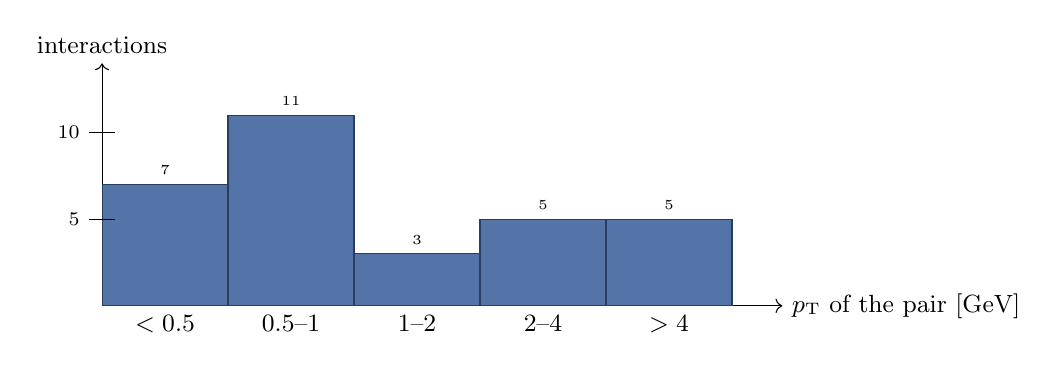
\begin{tikzpicture}[x=1.6cm, y=0.22cm]
\draw[->] (0,0) -- (5.4,0) node[right, font=\small] {$\pt$ of the pair [GeV]};
\draw[->] (0,0) -- (0,14) node[above, font=\small] {interactions};
\histbar{0}{7}\histbar{1}{11}\histbar{2}{3}\histbar{3}{5}\histbar{4}{5}
\foreach \x/\l in {0/$<0.5$, 1/0.5--1, 2/1--2, 3/2--4, 4/$>4$} \node[below, font=\small] at (\x+0.5,0) {\l};
\foreach \y in {5,10} \draw (0.1,\y) -- (-0.1,\y) node[left, font=\scriptsize] {\y};
\end{tikzpicture}
\caption{The 31 multiparton interactions of the event by the \pt{} of their outgoing parton pair (FWLite on
\code{step1\_GEN\_04\_MPI.root}, status-33 partons grouped by their mothers). The regulator of the CP5 tune at
$13.6\TeV$ is $\ptz=1.44\GeV$; the generation stops at \code{MultipartonInteractions:pTmin} $=0.2\GeV$
(Pythia8 default).}
\label{fig:04_mpipt}
\end{figure}

\paragraph{The regulator $\ptz$ and its energy dependence.}
The MPI cross section is regulated by $\ptz$, which Pythia8 scales with the collision energy,
\[
\ptz(\sqrt s)=\ptz^{\mathrm{Ref}}\left(\frac{\sqrt s}{E_{\mathrm{Ref}}}\right)^{\epsilon},
\qquad
\ptz^{\mathrm{Ref}}=1.41\GeV,\quad E_{\mathrm{Ref}}=7\TeV,\quad \epsilon=0.03344 ,
\]
with \code{MultipartonInteractions:pT0Ref} and \code{ecmPow} from the CP5 block
(\path{Configuration/Generator/python/MCTunes2017/PythiaCP5Settings_cfi.py}) and \code{ecmRef} at its Pythia8
default. This gives $\ptz=1.4395\GeV$ at $13\TeV$, $1.4417\GeV$ at $13.6\TeV$ (the ``pT0 = 1.44'' of the
initialisation in the log) and $1.4431\GeV$ at $14\TeV$: a $0.1\%$ step from Run~3 to the HL-LHC. The same
initialisation prints what the regulator does: with $\ptz=1.44\GeV$ the integrated parton--parton cross section
above the cut-off is $\sigma_{\mathrm{int}}=500.67\mb$ against a non-diffractive $pp$ cross section
$\sigma_{\mathrm{ND}}=55.42\mb$; their ratio, 9.0, is the mean number of interactions per non-diffractive
collision before the impact-parameter weighting. The other CP5 MPI parameters are the matter profile
(\code{bProfile=2}, a double Gaussian with \code{coreRadius=0.7634} and \code{coreFraction=0.63}) and
$\alpha_s(M_Z)=0.118$ at NLO for the MPI, the showers and the hard process.

\begin{plainwords}[What a tune is]
Pythia8 cannot compute $\ptz$, the proton's matter profile or how often colour lines
reconnect; these are parameters fitted to data. CP5 (\code{Tune:pp 14}, Monash 2013, with the CMS changes of the
block above) was fitted by CMS in 2017 (CMS-GEN-17-001) to underlying-event and minimum-bias data at 7 and
$13\TeV$ with NNPDF3.1 at NNLO. Everything in this chapter except the hard process depends on them; the ``Up''/``Down'' variants of the block
(\code{pT0Ref} 1.407 and 1.46) are the tune uncertainty.
\end{plainwords}

\paragraph{Primordial $k_\mathrm{T}$.}
The partons inside a proton are not exactly collinear with it. Once the interleaved evolution is finished,
Pythia8 gives every incoming parton of every interaction a small transverse kick and takes the recoil from the
remnants: the 64 entries of status 61 are these 64 incoming partons, two per interaction, with a mean
$k_\mathrm{T}$ of $1.09\GeV$ (median $0.77\GeV$, largest $3.89\GeV$).\footnote{FWLite on
\code{step1\_GEN\_04\_MPI.root}, status-61 entries.} The outgoing partons of each interaction are then copied
with the kick included: the $b$ goes from $\pt=91.59$ to $91.74\GeV$, the $\bar b$ from 118.57 to
$116.36\GeV$, and the net $|\vec\pt(b)+\vec\pt(\bar b)|$ from 27.29 to $25.08\GeV$. In this file these final
copies have no daughters, so they are the status-1 partons of the record, the ones page~3 of the analyzer draws;
in chapter~\ref{ch:05_Had}, where they fragment, the same copies appear as status 62.

\begin{figure}[!tb]
\centering
\includegraphics[width=\textwidth]{04_MPI/out/genPartAnalyzer_04_MPI_page-3.png}
\caption{The event at the end of the parton level in the $\eta$--$\phi$ plane (\code{genPartAnalyzer\_04\_MPI.pdf},
page 3; marker size grows with $\log\pt$, the \pt{} is written for $\pt>5\GeV$): 169 partons with their primordial
$k_\mathrm{T}$, coloured by the scattering they belong to. Orange and green: the ISR (1) and FSR (11) partons of
the hard process, the same as in figure~\ref{fig:04_showers}(b), with the $b$ at $91.7\GeV$ and the $\bar b$ at
$116.4\GeV$. Cyan: the 31 multiparton interactions, squares their 61 outgoing partons, triangles the 25 ISR (up)
and 56 FSR (down) emissions of their showers, soft and spread over the whole plane. Grey diamonds: the 13 beam
remnants, 11 of them at $\abseta>3.5$; 16 partons beyond $\abseta=6$ are crosses on the border. Dashed: the cones
$\Delta R<0.4$, $127.3\GeV$ around the $b$, of which $6.9\GeV$ from the underlying event (UE: MPI and remnants),
and $117.1\GeV$ around the $\bar b$ (UE $0.8\GeV$); the inset magnifies the $b$ cone, its UE partons in cyan. The
magenta star is $\vec\pt(b)+\vec\pt(\bar b)$, the recoil of the \bbbar{} pair against its radiation: $25.1\GeV$
($27.3\GeV$ before the primordial $k_\mathrm{T}$).}
\label{fig:04_display}
\end{figure}

\paragraph{Colour reconnection.}
With 32 interactions the event has 32 colour-connected systems stretched between the two remnants. Pythia8's
MPI-based colour reconnection (\code{ColourReconnection:mode} at its default 0, CP5 strength \code{range=5.176})
merges the colour lines of the softer interactions with the harder ones, which shortens the strings and reduces
the number of hadrons. It acts on colour indices, which \code{genParticles} does not store; its effect appears
only when the strings break in chapter~\ref{ch:05_Had}, and nothing in the momenta of this record changes.

\paragraph{Beam remnants, and why the record still has $13\,600\GeV$.}
Each proton gave one parton to each of the 32 interactions; what is left is the beam remnant. Pythia8 builds it so that the proton's flavour content is restored: a
valence quark taken out leaves a diquark (a $ud$ or $uu$ pair, pdg 2101, 2103 or 2203), a sea quark taken out
leaves its antiquark partner, and so on. This event has 13 remnant partons, all single quarks or antiquarks
($u$, $d$, $\bar u$, $\bar d$, $\bar s$) and no diquark: with 32 partons extracted from each proton,
including the valence $u$ at $x=0.39$ of the hard process, no valence pair was left intact. They carry
$1783.0\GeV$ of energy and $6.5\GeV$ of scalar \pt{} in total; eleven of the 13 have $\abseta>3.5$ and the
two hardest, 416 and $350\GeV$, are at $\eta=7.0$ and $-7.3$, in the beam pipe.\footnote{FWLite on
\code{step1\_GEN\_04\_MPI.root}: the status-1 partons whose mother is a beam proton (status 4). In chapter~\ref{ch:05_Had}
the same 13 partons carry status 63.} Energy and momentum are conserved exactly: the 169 final-state partons sum
to $E=13\,600.0\GeV$ and $\sum\vec\pt=0$, because the remnants take what the interactions did not, and the
primordial-$k_\mathrm{T}$ recoil is given to them. Of the $13.6\TeV$, $2862.2\GeV$ sits in the 14 partons of
the hard process and its showers, $8954.8\GeV$ in the 142 partons of the MPI and their showers, and
$1783.0\GeV$ in the remnants; the hard system has $266.8\GeV$ of scalar \pt, the MPI $207.9\GeV$, the remnants
$6.5\GeV$.

\paragraph{What reaches the two $b$ jets.}
For the jet chapters, how much MPI activity lands near the $b$ and $\bar b$? The cones of
figure~\ref{fig:04_display}, $\Delta R<0.4$ around the final $b$ ($\eta=-1.57$, $\phi=-2.08$) and $\bar b$,
answer it parton by parton. The $b$ cone holds nine partons with a vector \pt{} of $127.3\GeV$: the six of the
hard process of figure~\ref{fig:04_showers}(b) ($120.6\GeV$ of scalar \pt) and three of the \emph{underlying
event} (UE: the partons of the MPI and the remnants), $6.9\GeV$, a $\bar u$ of $3.7\GeV$ and a gluon of
$2.3\GeV$ from the initial-state showers of two MPI and a gluon of $0.9\GeV$ radiated by the $\bar c$ of a third.
That $\bar c$ itself, now $0.8\GeV$, is the one UE parton in the $\bar b$ cone, next to the $\bar b$ of
$116.4\GeV$: one soft interaction (a $\bar c$ and a gluon of $1.9\GeV$) puts \pt{} into both
jets.\footnote{\code{genPartAnalyzer\_04\_MPI.log} (the ``cone'' lines of stage 3 give the scattering of every
member), \code{ledger\_04\_MPI.txt}; the ancestry of the UE partons from FWLite (companion, section 4.6).} In the
tracker acceptance, $\abseta<2.5$, the 80 final-state partons are 13 from the hard system ($150.5\GeV$ of \pt), 66 from the MPI ($103.8\GeV$) and one remnant quark ($0.3\GeV$): the underlying
event of this collision is two fifths of the central \pt, spread over the whole $\eta$--$\phi$ plane, 5\% of
the \pt{} inside the cone of the $b$ and less than one per cent inside that of the $\bar b$.

\section{Ledger and display}

\begin{table}[htb]
\centering\small
\caption{Ledger of the stage: the record and the final state (status 1) before (chapter~\ref{ch:02_PS},
\code{ledger\_02\_PS.txt}) and after (\code{ledger\_04\_MPI.txt}) multiparton interactions and beam remnants. Regions:
tracker ($\abseta<2.5$), the gap to the HF edge, the forward calorimeter, and $\abseta>5.2$, which Geant4 is not
given (chapter~\ref{ch:09_G4}). Cones: the status-1 partons within $\Delta R<0.4$ of the final $b$ and $\bar b$
(\code{genLedger.py}), with their vector \pt.}
\label{tab:04_ledger}
\footnotesize\setlength{\tabcolsep}{3.2pt}
\begin{tabular}{lrrrrrrrrr}
\toprule
 & \multicolumn{3}{c}{chapter 02 (MPI off)} & \multicolumn{3}{c}{chapter 04 (MPI on)} & \multicolumn{3}{c}{difference} \\
\cmidrule(lr){2-4}\cmidrule(lr){5-7}\cmidrule(lr){8-10}
 & $n$ & $E$ [GeV] & \pt{} [GeV] & $n$ & $E$ [GeV] & \pt{} [GeV] & $n$ & $E$ [GeV] & \pt{} [GeV] \\
\midrule
record (all entries) & 34 & & & 745 & & & $+711$ & & \\
\quad hard process (21--29) & 4 & & & 4 & & & 0 & & \\
\quad MPI (31--39) & 0 & & & 124 & & & $+124$ & & \\
\quad ISR (41--49) & 0 & & & 190 & & & $+190$ & & \\
\quad FSR (51--59) & 15 & & & 192 & & & $+177$ & & \\
\quad primordial $k_\mathrm{T}$, remnants (61--69) & 2 & & & 64 & & & $+62$ & & \\
\midrule
final state (status 1), all partons & 11 & 13600.0 & 230.7 & 169 & 13600.0 & 481.2 & $+158$ & 0.0 & $+250.5$ \\
\quad $\abseta<2.5$ & 6 & 256.9 & 113.7 & 80 & 642.1 & 254.5 & $+74$ & $+385.2$ & $+140.8$ \\
\quad $2.5<\abseta<3.0$ & 0 & 0.0 & 0.0 & 17 & 190.5 & 22.3 & $+17$ & $+190.5$ & $+22.3$ \\
\quad $3.0<\abseta<5.2$ & 1 & 2413.9 & 114.0 & 50 & 4907.4 & 183.0 & $+49$ & $+2493.5$ & $+69.0$ \\
\quad $5.2<\abseta<5.5$ & 0 & 0.0 & 0.0 & 3 & 245.3 & 2.5 & $+3$ & $+245.3$ & $+2.5$ \\
\quad $\abseta>5.5$ & 4 & 10929.2 & 2.9 & 19 & 7614.7 & 18.9 & $+15$ & $-3314.5$ & $+16.0$ \\
\quad visible ($\abseta<5.2$) & 7 & 2670.8 & 227.8 & 147 & 5740.0 & 459.8 & $+140$ & $+3069.2$ & $+232.0$ \\
\midrule
$b$ cone $\Delta R<0.4$ & 6 & 256.9 & 113.6 & 9 & 325.3 & 127.3 & $+3$ & $+68.4$ & $+13.7$ \\
$\bar b$ cone $\Delta R<0.4$ & 1 & 2413.9 & 114.0 & 2 & 2485.9 & 117.1 & $+1$ & $+72.0$ & $+3.1$ \\
\bottomrule
\end{tabular}
\end{table}

Table~\ref{tab:04_ledger} closes the ledger of the stage against chapter~\ref{ch:02_PS}
(chapter~\ref{ch:03_MnM} only copied the file). The stage adds 158 final-state partons and $250.5\GeV$ of scalar
\pt{} but no energy: the $13\,600\GeV$ move from $\abseta>5.5$, where the two spectators of
chapter~\ref{ch:02_PS} sat with $10\,929\GeV$, into $3.0<\abseta<5.2$ ($+2493.5\GeV$, the MPI partons and their
showers at small $x$) and the tracker ($+385.2\GeV$); the visible energy doubles from 2670.8 to $5740.0\GeV$, and
$2.5<\abseta<3.0$, empty before, receives 17 partons and $190.5\GeV$. The two cone rows are the jet side of the
ledger: the $b$ cone gains $13.7\GeV$, half of it the underlying event ($6.9\GeV$) and half the other shower
draw (its hard-process partons carry $120.5\GeV$ of vector \pt{} instead of $113.6\GeV$).

Figure~\ref{fig:04_display} is the $\eta$--$\phi$ display at the end of the stage: 169 partons, each coloured
by the scattering it belongs to (the analyzer follows its mothers up to a scattering, as the FWLite count of
table~\ref{tab:04_shower}): 14 of the hard process and its showers, 142 of the MPI and their showers, 13 beam
remnants. The 14 are the partons of figure~\ref{fig:04_showers}(b) ($b$, $\bar b$, one ISR and 11 FSR partons,
same colours), moved only by the primordial $k_\mathrm{T}$: the same event, with the rest of the collision
added. The 142 are the 61 outgoing partons of the 31 interactions (a parton that radiated keeps its label) and
the 25 ISR and 56 FSR emissions of their showers.


\section{Open problems for Phase-2}



\paragraph{CP5 is a 2017 tune extrapolated to $14\TeV$ through one exponent.}
The block used by the fragment of this book, \path{Configuration/Generator/python/MCTunes2017/PythiaCP5Settings_cfi.py},
sets \code{pT0Ref=1.41}, \code{ecmPow=0.03344}, \code{coreRadius=0.7634}, \code{coreFraction=0.63} and
\code{ColourReconnection:range=5.176}; these were fitted to 7 and $13\TeV$ data (CMS-GEN-17-001; the release
records only the tune name), and the only handle that knows about the beam energy is \code{ecmPow}, which moves $\ptz$ from $1.4395\GeV$ at $13\TeV$ to
$1.4431\GeV$ at $14\TeV$. The Pythia8 default is \code{ecmPow=0.215} (Monash); CP5's value, six times smaller,
means an almost energy-independent regulator, so the MPI activity in CP5 grows with $\sqrt s$ nearly as fast as
the parton densities at small $x$ do. No $14\TeV$ measurement tests this extrapolation yet; the release contains no $14\TeV$ tune, and the directory \path{MCTunes2017/} holds only the
CP1--CP5 blocks of 2017 with their ``Up''/``Down'' variants and the two colour-reconnection alternatives
\path{PythiaCP5CR1TuneSettings_cfi.py} (\code{ColourReconnection:mode=1}, \code{BeamRemnants:remnantMode=1},
\code{pT0Ref=1.375}) and \path{PythiaCP5CR2TuneSettings_cfi.py} (\code{mode=2}, \code{pT0Ref=1.454},
\code{ecmPow=0.0555}), alternatives for systematic studies, not replacements. What could not be established:
which data entered the CP5 fit (the release records only the tune name) and whether a newer CMS tune exists
outside the release; inside it there is none, and no $14\TeV$ or Phase-2 variant of the MPI parameters.

\paragraph{The only Run-3 update is the total cross section, and most fragments do not use it.}
The release has a second directory, \path{Configuration/Generator/python/MCTunesRun3ECM13p6TeV/}, whose
\path{PythiaCP5Settings_cfi.py} differs from the 2017 file in two lines only: \code{SigmaTotal:sigmaEl}
(22.08 instead of $21.89\mb$) and \code{SigmaTotal:sigmaTot} (101.037 instead of $100.309\mb$). With
\code{SigmaTotal:mode = 0} Pythia8 takes these total and elastic cross sections as fixed numbers at whatever beam
energy is set, and derives from them the non-diffractive cross section that normalises the MPI rate, the
$\sigma_{\mathrm{ND}}=55.42\mb$ printed at $13.6\TeV$ in \code{step1\_GEN\_04\_MPI.log}. Our fragment and the
release's minimum-bias fragment \path{Configuration/Generator/python/MinBias_14TeV_pythia8_TuneCP5_cfi.py} (the
pileup library of chapter~\ref{ch:08_PU}, and the \path{RelValMinBias_14TeV} input that
\path{Configuration/PyReleaseValidation/python/relval_steps.py} mixes at \path{AVE_200_BX_25ns} for the Phase-2
workflows) both import the 2017 block, i.e.\ the $13\TeV$ cross sections; only six B-physics and soft-QCD
fragments import the $13.6\TeV$ one, and no file in the release carries $14\TeV$ values. At PU~200 a per-cent
change in the MPI activity of one minimum-bias collision is a per-cent change of the whole pileup energy in every
crossing.

\paragraph{Pileup is MPI without a hard process.}
The minimum-bias collisions of chapter~\ref{ch:08_PU} are generated with \code{SoftQCD:inelastic = on} and the
same CP5 block: their 7.0 interactions on average (\code{genstats\_08\_PU.txt}) come from the same $\ptz$,
matter profile and colour reconnection as the 31 interactions of this event, so the pileup jets of
chapter~\ref{ch:08_PU} are made of exactly the objects studied here. Table~\ref{tab:04_ledger} shows where they
go: 17 partons with $190.5\GeV$ added in $2.5<\abseta<3.0$ and 49 with $2493.5\GeV$ in $3.0<\abseta<5.2$, the
HGCal endcap and the extended Phase-2 tracker ($\abseta<4.0$), the regions Run~3 measures least precisely and
that constrained the tune the least.



%% chapter_05_Had.tex -- chapter 05 of the JitJet book: hadronisation (Lund strings), HadronLevel:Hadronize on, Decay off.
% Numbers: test/05_Had/out/ledger_05_Had.txt, genPartAnalyzer_05_Had.log, step1_GEN_05_Had.log, and the FWLite counts of
% doc/chapter/chapter_05_Had.md (section 4) read from step1_GEN_05_Had.root; the parton level of chapter 04 from
% test/04_MPI/out/ledger_04_MPI.txt.
\chapter{05 -- Hadronisation: the 169 partons become 320 primary hadrons}
\label{ch:05_Had}

\section{What this chapter is about}
Up to chapter~\ref{ch:04_MPI} the event is made of quarks and gluons. Nothing with a colour charge has ever
reached a detector: when the partons fly apart, the colour field between them does not spread out like an
electric field but is squeezed into a narrow tube, a \emph{string}, whose energy grows with its length until it
is cheaper to create a new quark--antiquark pair from the field than to stretch it further. This is
hadronisation, and in Pythia8 it is done by the Lund string model, switched on in this chapter with
\code{HadronLevel:Hadronize = on} while the decays of the hadrons stay off (\code{HadronLevel:Decay = off}).
The final state of this chapter is therefore the set of \emph{primary hadrons}: the particles the strings
produce directly, including the unstable ones ($\pi^0$, $\rho$, $\omega$, $K^*$, $\Delta$, $B^*$) that the next
chapter will decay. There are 320 of them, made from the 169 partons of chapter~\ref{ch:04_MPI}, and they carry
exactly the $13600.0\GeV$ of the two protons.\footnote{All numbers of this chapter are read from
\code{test/05\_Had/out/}: \code{ledger\_05\_Had.txt} (the record and the final state by kind and region),
\code{genPartAnalyzer\_05\_Had.log} (the $b$ and $\bar b$ chains, stage by stage), \code{step1\_GEN\_05\_Had.log}
(the Pythia8 settings and the hard process) and the FWLite counts of the companion
\code{doc/chapter/chapter\_05\_Had.md}, section~4, read from \code{step1\_GEN\_05\_Had.root}.}

The chapter follows the two partons of the hard process to the end of their colour strings: the $b$ quark
with $\pt=91.7\GeV$ becomes a $B^-$ meson with $\pt=94.3\GeV$, the $\bar b$ with $116.4\GeV$ a $B^{*+}$ with
$114.2\GeV$, both within $\Delta R<0.01$ of the quark. That a $b$ hadron keeps almost all of the momentum of
its quark is the single most important fact of this chapter for jet physics: it is what makes a $b$ jet
different from a light-quark or a gluon jet, and it is set by one fragmentation function and two numbers
that CMS has never tuned.

\section{From the previous chapter}
Chapter~\ref{ch:04_MPI} ended with 169 partons in the final state (status~1 in that file), counted there by the
scattering they belong to: the two $b$ quarks with the 12 ISR and FSR partons of the hard process, 142 partons of
the 31 additional multiparton interactions and their showers, and 13 beam-remnant quarks, all colour connected,
with $\sum E=13600.0\GeV$ and $\sum\pt=481.2\GeV$; the cone $\Delta R<0.4$ around the $b$ held $127.3\GeV$,
$6.9\GeV$ of it from the underlying event, the one around the $\bar b$ $117.1\GeV$. This chapter regenerates the same event with the same seeds,
so the parton level is identical: the same 169 partons are in this file with status~62 (156 outgoing
partons with their primordial $k_T$ included) and 63 (13 beam remnants), with the same $13600.0\GeV$ and
$481.2\GeV$, the same $b$ quark ($\pt=91.74\GeV$, $\eta=-1.57$) and $\bar b$ ($116.36\GeV$, $\eta=-3.75$).
Everything up to status~63 is kept. New in the record are 165 entries with status 71--79, the partons as they
enter the strings, reordered so that every colour singlet is contiguous (120 copies with status~71 and 45 partons
with status~73, each made by joining two very nearby ones), and the 320
primary hadrons: the record grows from 745 to 1230 entries. Gone is every free colour charge: the final
state of this chapter has 169 charged and 151 neutral hadrons and not a single parton.

\begin{plainwords}[Why hadronisation cannot be computed and must be modelled]
The parton shower stops at a scale of about $1\GeV$ (\code{TimeShower:pTmin}, raised to $0.611\GeV$ in the
log), where the strong coupling becomes too large for perturbation theory. From there to the hadrons there
is no formula, only a model with parameters fitted to data. Pythia8 uses the Lund string model, in which the colour field between a quark and an antiquark (or between the colour
ends of a chain of gluons) is a string with a constant tension $\kappa\approx1\GeV/\mathrm{fm}$. The string
breaks by creating $q\bar q$ pairs along its length, and each piece between two breaks becomes one hadron.
The model has a handful of parameters (which flavour is created at a break, how much momentum a hadron
takes, how much transverse momentum it gets); they were fitted once to $e^+e^-$ data at LEP, and CMS
inherits them unchanged through the tune CP5.
\end{plainwords}

\section{The numbers of the event}
\paragraph{The strings.}
Grouping the 320 primary hadrons by the set of partons they descend from gives 26 colour singlets, from
2 to 42 hadrons each (mean~12.3), listed in the companion. Twenty-one are ordinary strings with a quark at
one end and an antiquark at the other, from a plain $q\bar q$ pair up to chains of 10, 17 and 18 gluons
between the ends; two are \emph{junction} strings with three quark ends ($uud$ and $uds$), the leftovers of
the two proton remnants; three are \emph{ministrings}, $q\bar q$ pairs of mass $1.0$, $1.3$ and $1.5\GeV$, less
than \code{HadronLevel:mStringMin} $=1\GeV$ above the constituent masses of their two quarks, too light to
fragment and turned directly into two hadrons each. The most energetic string carries $3630.7\GeV$ along the
beam (a $u\bar d$ pair with 18 gluons, 42 hadrons); the heaviest has a mass of $1083.9\GeV$ (33 hadrons).
Table~\ref{tab:05strings} gives the two strings of the hard process: the $b$ quark is colour connected
through three gluons to an $\bar s$ quark created in the shower, a string of mass $12.8\GeV$ that gives six
hadrons; the $\bar b$ sits at the end of a plain two-parton string with a $d$ quark from the other side of
the event, of mass $99.6\GeV$, that gives only four hadrons because the $\bar b$ end keeps almost everything.

\begin{table}[htbp]
\centering\small
\caption{The two strings of the hard process and their primary hadrons (FWLite, \code{step1\_GEN\_05\_Had.root};
quark momenta of status~62, hadron momenta of the status-1 primary hadrons; $x_E=E(\text{hadron})/E(\text{quark})$).}
\label{tab:05strings}
\setlength{\tabcolsep}{4pt}
\begin{tabular}{lrrrrrl}
\toprule
string & quark \pt & quark $E$ & $M$ & $E$ & $n_{\rm had}$ & primary hadrons (GeV) \\
\midrule
$b\,g\,g\,g\,\bar s$ & 91.74 & 230.0 & 12.8 & 285.1 & 6 & $B^-$: $\pt=94.28$, $E=235.9$, $x_E=1.025$ \\
 & & & & & & $+\ \pi^0\,\pi^+\,\pi^0\,\pi^0\,K^0$ (\pt{} 0.9 to 7.2) \\
$d\,\bar b$ & 116.36 & 2469.9 & 99.6 & 2471.2 & 4 & $B^{*+}$: $\pt=114.17$, $E=2421.4$, $x_E=0.980$ \\
 & & & & & & $+\ \pi^-\,K^+\,K^{*-}$ (50 GeV between them) \\
\bottomrule
\end{tabular}
\end{table}

\paragraph{The fragmentation function and the $b$ hadrons.}
At each break the model draws the fraction $z$ of the remaining light-cone momentum of the string end that
the new hadron takes, from the Lund symmetric fragmentation function
\[
  f(z) \propto \frac{1}{z}\,(1-z)^{a}\,\exp\!\left(-\frac{b\,m_T^2}{z}\right),\qquad
  m_T^2 = m^2 + \pt^2 ,
\]
with $a=0.68$ (\code{StringZ:aLund}) and $b=0.98\GeV^{-2}$ (\code{StringZ:bLund}). For a light hadron
($m_T\approx0.5\GeV$) the exponential hardly matters and $f(z)$ peaks at small $z$: a light string end hands
out its momentum in many small steps, which is why the $u\bar d$ string of $3630.7\GeV$ gives 42 hadrons. For a
hadron containing the heavy quark at the string end, $m_T^2\approx m_B^2\approx28\GeV^2$ makes the exponential
kill all small $z$; in addition Pythia8 applies the Bowler modification for heavy quarks, an extra factor
$1/z^{\,r_Q\,b\,m_Q^2}$ with $r_b=0.855$ (\code{StringZ:rFactB}) and the $b$ mass $m_b=4.8\GeV$ of the hard
process. The result is a function that peaks at $z\approx0.93$ (mean $0.89$, for $m_T=m_B$) and vanishes at $z\to0$: the first
hadron produced at a $b$ end takes most of the string momentum, and the light hadrons that share the string
with it are soft. The event shows exactly this. The $B^-$ carries $x_E=1.025$ of the energy of its $b$ quark
and 83\% of the energy of the whole five-parton string ($235.9$ of $285.1\GeV$); it can carry \emph{more} than
its quark because the string also holds the three gluons and the $\bar s$ end, whose momentum is shared along
the string. The $B^{*+}$ carries $x_E=0.980$ of its $\bar b$ and leaves $50\GeV$ to three light hadrons. Both $b$
hadrons are within $\Delta R$ of $0.009$ and $0.001$ of their quark: hadronisation does not move the $b$
direction, it only dresses it. The five light hadrons of the $b$ string have $\pt$ between $0.9$ and
$7.2\GeV$.

\paragraph{The cones around the two $b$ hadrons.}
The dashed circles of figure~\ref{fig:05display} are the cones $\Delta R<0.4$ of chapters~\ref{ch:02_PS}
and~\ref{ch:04_MPI}, now around the $B^-$ and the $B^{*+}$, and the inset magnifies the cone of the $B^-$, whose
hadrons the main frame cannot separate. It holds nine primary hadrons with a vector \pt{} of $114.4\GeV$: the
$B^-$ and eight light hadrons with $\sum\pt=20.4\GeV$, five $\pi^0$ ($7.2$, $6.5$, $2.8$, $2.0$ and $0.5\GeV$), a
$K^0$, a $\bar K^{*0}$ and a $\pi^-$; the cone of the $B^{*+}$ holds a single $K^{*-}$ of $1.8\GeV$ besides it,
$116.0\GeV$. At parton level the same two cones held $127.3$ and $117.1\GeV$: hadronisation takes $12.8\GeV$
out of the $b$ cone. A cone is not a string: the hadrons are made along the strings, and several strings pass
through this cone (the $b$ string and those of the ISR and MPI partons that were inside it). Four hadrons just
outside the circle carry about as much as the cone lost: a $\bar p$ of $5.3\GeV$ at $\Delta R=0.45$, a
$\Delta^{++}$ of $2.8\GeV$ at $0.51$, and a $\rho^+$ and a $\pi^+$ of $2.4\GeV$ at $0.46$ and $0.42$, the $\pi^+$
one of the five light hadrons of the $b$ string.\footnote{\code{genPartAnalyzer\_05\_Had.log} (the ``cone'' line
of stage 4) and \code{ledger\_05\_Had.txt}; the hadrons outside the cone from FWLite (companion, section 4).}
This loss out of the cone is what the jet energy corrections later call the hadronisation part of the
out-of-cone showering; it is a property of the Lund strings, and of their parameters.

Which hadron is made at a break is the second draw of the model: a $q\bar q$ pair is created with
probability $u:d:s = 1:1:0.217$ (\code{StringFlav:probStoUD}), a diquark pair with probability 0.081 relative
to a quark pair (\code{StringFlav:probQQtoQ}, the source of the 34 baryons), and the new meson is a vector
rather than a pseudoscalar with a flavour-dependent ratio: $0.5$ for $u,d$ (\code{StringFlav:mesonUDvector}),
$0.55$ for $s$, $2.2$ for $b$ (\code{StringFlav:mesonBvector}). The last number is why the $\bar b$ became a
$B^{*+}$ and not a $B^+$: with a vector-to-pseudoscalar ratio of 2.2 the excited state is drawn 69\% of the
time, and the $B^{*+}$ will decay to $B^+\gamma$ in chapter~\ref{ch:06_Decay}.

\begin{plainwords}[Why a $b$ jet is not a light jet]
A light quark hands its momentum to a long chain of pions, each with a few per cent of it; a $b$ quark hands
80--100\% of it to one $B$ hadron in one step, because the Lund function with the Bowler term makes small $z$
impossible for a heavy end. A $b$ jet is therefore one heavy particle plus a few soft hadrons, and the jet
response of the detector, the $b$-tagging, the fraction of energy lost in neutrinos when the $B$ decays
(chapter~\ref{ch:06_Decay}) all follow from this one function and the two numbers $r_b$ and $b$, fitted to
$e^+e^-$ data at the $Z$ pole.
\end{plainwords}

\paragraph{The species.}
Table~\ref{tab:05species} counts the 320 primary hadrons: 286 mesons and 34 baryons, two of
them with a $b$ quark and two with a $c$ quark (a $\bar D^0$ and a $D^{*+}$ from a $c\bar c$ pair created in the
shower, with $\pt$ of only $2.0$ and $1.9\GeV$). The pions, charged and neutral, are 132; the vector mesons
$\rho$ and $\omega$, 77, are about half of the 149 light pseudoscalars ($\pi$, $\eta$, $\eta'$), which is the
vector-to-pseudoscalar ratio of 0.5 at work (one spin state for the pseudoscalar against three for the vector,
suppressed by their mass); the
kaons and $K^*$, 56, reflect the strangeness suppression 0.217. The spectrum is soft: 124 hadrons have
$\pt<0.5\GeV$, 226 have $\pt<1\GeV$, only 8 have $\pt>5\GeV$ and only the two $B$ hadrons exceed $10\GeV$.
The transverse momentum of a light hadron comes from the Gaussian $\pt$ kick of each string break, of width
$\sigma=0.335\GeV$ (\code{StringPT:sigma}); this is where the $+24.5\GeV$ of scalar $\sum\pt$ of the ledger
comes from, $0.16\GeV$ per additional particle.

\begin{table}[htbp]
\centering\small
\caption{The 320 primary hadrons by class (FWLite count of the status-1 particles of
\code{step1\_GEN\_05\_Had.root}, listed by species in the companion, section~4).}
\label{tab:05species}
\begin{tabular}{lrrrl}
\toprule
class & $n$ & $\sum E$ [GeV] & $\sum\pt$ [GeV] & species \\
\midrule
pions & 132 & 2736.5 & 108.5 & $\pi^\pm$ 86, $\pi^0$ 46 \\
light vector and $\eta$ mesons & 94 & 3169.2 & 99.0 & $\rho^\pm$ 34, $\rho^0$ 25, $\omega$ 18, $\eta$ 14, $\eta'$ 3 \\
kaons & 39 & 1173.6 & 39.0 & $K^\pm$ 22, $K^0$ 17 \\
$K^*$ & 17 & 414.8 & 13.1 & $K^{*0}$ 9, $K^{*\pm}$ 8 \\
nucleons & 19 & 2888.6 & 18.0 & $n$ 10, $p$ 9 \\
other light baryons & 15 & 523.8 & 15.7 & $\Lambda$ 3, $\Sigma$ 3, $\Sigma^*$ 4, $\Delta$ 5 \\
charm hadrons & 2 & 36.2 & 3.9 & $\bar D^0$, $D^{*+}$ \\
bottom hadrons & 2 & 2657.3 & 208.5 & $B^-$, $B^{*+}$ \\
\midrule
all & 320 & 13600.0 & 505.7 & 169 charged, 151 neutral \\
\bottomrule
\end{tabular}
\end{table}


\paragraph{Energy is conserved exactly.}
The ledger of chapter~\ref{ch:04_MPI} closed at $13600.0\GeV$ and this one closes at $13600.0\GeV$: not
approximately, but string by string. String fragmentation takes the total four-momentum of each colour
singlet and distributes it among its hadrons; the last two hadrons of every string are made together from
whatever four-momentum is left (the ``final joining''), so that each string conserves energy and momentum
by construction. In this event the 26 strings have $|\Delta E|<0.5\MeV$ each between their partons and
their hadrons. What hadronisation does create is mass: the 169 partons had $\sum m=30.8\GeV$ ($9.6\GeV$ in the
two $b$ quarks, $16.7\GeV$ in the 39 other quarks of the showers and the MPI, $4.5\GeV$ in the 13 remnant
quarks; the gluons are massless), the 320 hadrons have $\sum m=176.7\GeV$, taken from the
kinetic energy of the strings. Pythia8 then checks the sum over the whole event and would reject it if the
mismatch exceeded \code{Check:epTolErr}, set to $0.01$ by CMS in
\path{Configuration/Generator/python/Pythia8CommonSettings_cfi.py} (Pythia8 default $10^{-4}$); the check never
fires here.

\paragraph{Colour reconnection.}
Before the strings are formed, Pythia8 may rearrange the colour connections between the 32 scattering systems
of the event (the hard process and 31 MPI): this is colour reconnection (CR), and in the MPI-based model used by
CP5 (\code{ColourReconnection:mode = 0}) a system of scale $\pt$ is merged into a harder one with probability
$(p_{\mathrm{T},0}^{\mathrm{rec}})^2/((p_{\mathrm{T},0}^{\mathrm{rec}})^2+\pt^2)$, with $p_{\mathrm{T},0}^{\mathrm{rec}}=\mathrm{range}\times p_{\mathrm{T},0}$. CP5 sets
\code{ColourReconnection:range = 5.176} (Pythia8 default 1.8, the largest change CP5 makes to the hadron level);
with the $p_{\mathrm{T},0}=1.44\GeV$ of this run (\path{step1_GEN_05_Had.log}) a system of $\pt\approx7.5\GeV$ is merged
half of the time, and the soft MPI systems almost always. CR shortens the total string length and so lowers
the number of hadrons per MPI; it is the knob with which the tune reproduces the measured $\langle\pt\rangle$
versus charged multiplicity. It is why the 32 systems of this event end up as 26 strings, several with ten
and more gluons from different scatterings. It leaves no separate status code in the record (status~79
belongs to the other CR models): its effect is in the colour indices of the status-62 partons.

\section{Ledger and display}
Table~\ref{tab:05ledger} is the ledger of the stage: the 169 partons before (identical to the final state of
chapter~\ref{ch:04_MPI}, and present in this file as status~62 and 63) against the 320 primary hadrons after.
The energy is unchanged in total but moves between regions: the forward strings span many units of
rapidity and their hadrons land where the string, not the parton, was. The region beyond $\abseta=5.5$ loses
$604.6\GeV$ and the ring $5.2<\abseta<5.5$ gains $565.4\GeV$ (fifteen hadrons there instead of three
partons), while the tracker region gains 61 particles and $42.5\GeV$. The visible energy within $\abseta<5.2$
goes from $5740.0$ to $5779.2\GeV$, less than 1\% of a change; the scalar $\sum\pt$ rises by 5\% for the
reason given above. The two cone rows are the jet side of the ledger: hadronisation takes $12.8\GeV$ of \pt{}
out of the $b$ cone and $1.1\GeV$ out of the $\bar b$ cone. Figure~\ref{fig:05display} is the $\eta$--$\phi$
display of the primary hadrons: the $B^-$ at $(-1.57,-2.09)$ and the $B^{*+}$ at $(-3.75,1.01)$ are the only two
large markers, each in its cone; the rest is the soft spray of the 26 strings, denser at large $\abseta$, with
25 hadrons beyond $\abseta=6$ drawn on the border.

\begin{plainwords}[What a detector will see of this stage]
Nothing of the strings themselves, only the hadrons, and only after the next chapter has decayed the unstable
ones. But the split made here decides what kind of energy arrives: 169 charged hadrons with $355\GeV$ of \pt{}
for the tracker, 151 neutral ones with $151\GeV$, among them 46 $\pi^0$ that will become photons in the
electromagnetic calorimeter. The jet energy scale is the detector response to this mixture, and the mixture is
set by the Lund parameters.
\end{plainwords}

\begin{center}\begin{minipage}{\textwidth}\centering\footnotesize
\captionof{table}{Ledger of the hadronisation stage, event 1:1:1. Before: the 169 partons of chapter~\ref{ch:04_MPI}
(\code{test/04\_MPI/out/ledger\_04\_MPI.txt}, final state), after: the 320 primary hadrons
(\code{test/05\_Had/out/ledger\_05\_Had.txt}); the $b$ and $\bar b$ rows from \code{genPartAnalyzer\_05\_Had.log},
the masses from the FWLite count of the companion. $E$ and \pt{} in GeV, \pt{} scalar sums, except in the cone
rows: the final-state particles within $\Delta R<0.4$ of the last copy of the $b$ and $\bar b$ quark
(\code{genLedger.py}), vector \pt; differences before rounding.}
\label{tab:05ledger}
\begin{tabular}{lrrrrrrrrr}
\toprule
 & \multicolumn{3}{c}{before (partons)} & \multicolumn{3}{c}{after (primary hadrons)} & \multicolumn{3}{c}{difference} \\
\cmidrule(lr){2-4}\cmidrule(lr){5-7}\cmidrule(lr){8-10}
 & $n$ & $\sum E$ & $\sum\pt$ & $n$ & $\sum E$ & $\sum\pt$ & $n$ & $\sum E$ & $\sum\pt$ \\
\midrule
final state & 169 & 13600.0 & 481.2 & 320 & 13600.0 & 505.7 & $+151$ & $0.0$ & $+24.5$ \\
\quad partons & 169 & 13600.0 & 481.2 & 0 & 0.0 & 0.0 & $-169$ & $-13600.0$ & $-481.2$ \\
\quad charged hadrons & 0 & 0.0 & 0.0 & 169 & 8863.8 & 355.0 & $+169$ & $+8863.8$ & $+355.0$ \\
\quad neutral hadrons & 0 & 0.0 & 0.0 & 151 & 4736.2 & 150.7 & $+151$ & $+4736.2$ & $+150.7$ \\
\midrule
$\abseta<2.5$ (tracker) & 80 & 642.1 & 254.5 & 141 & 684.6 & 259.9 & $+61$ & $+42.5$ & $+5.4$ \\
$2.5<\abseta<3.0$ & 17 & 190.5 & 22.3 & 30 & 196.8 & 24.6 & $+13$ & $+6.3$ & $+2.3$ \\
$3.0<\abseta<5.2$ (HF) & 50 & 4907.4 & 183.0 & 94 & 4897.9 & 192.4 & $+44$ & $-9.5$ & $+9.4$ \\
$5.2<\abseta<5.5$ & 3 & 245.3 & 2.5 & 15 & 810.7 & 7.9 & $+12$ & $+565.4$ & $+5.4$ \\
$\abseta>5.5$ & 19 & 7614.7 & 18.9 & 40 & 7010.1 & 20.9 & $+21$ & $-604.6$ & $+2.0$ \\
visible, $\abseta<5.2$ & 147 & 5740.0 & 459.8 & 265 & 5779.2 & 476.9 & $+118$ & $+39.2$ & $+17.1$ \\
\midrule
$\sum m$ of the final state & & 30.8 & & & 176.7 & & & $+145.9$ & \\
$b$ quark $\to$ $B^-$, \pt & & & 91.74 & & & 94.28 & & & $+2.54$ \\
$\bar b$ quark $\to$ $B^{*+}$, \pt & & & 116.36 & & & 114.17 & & & $-2.18$ \\
$|\vec\pt(b)+\vec\pt(\bar b)|$ & & & 25.08 & & & 20.30 & & & $-4.77$ \\
\midrule
$b$ cone $\Delta R<0.4$ & 9 & 325.3 & 127.3 & 9 & 290.6 & 114.4 & 0 & $-34.8$ & $-12.8$ \\
$\bar b$ cone $\Delta R<0.4$ & 2 & 2485.9 & 117.1 & 2 & 2465.3 & 116.0 & 0 & $-20.6$ & $-1.1$ \\
\bottomrule
\end{tabular}
\end{minipage}\end{center}

\begin{figure}[htbp]
\centering
\includegraphics[width=\textwidth]{05_Had/out/genPartAnalyzer_05_Had_page-4.png}
\caption{The event after hadronisation (\code{test/05\_Had/out/genPartAnalyzer\_05\_Had\_page-4.png}, page 4 of
\code{genPartAnalyzer\_05\_Had.pdf}): the 320 primary hadrons in $\eta$--$\phi$, marker size $\propto\log\pt$,
the $B^-$ (red) and the $B^{*+}$ (blue) matched to the $b$ and $\bar b$ chains, the star their vector sum. Dashed:
the cones $\Delta R<0.4$ (analyzer option \code{coneR}), $114.4\GeV$ around the $B^-$ (nine hadrons) and
$116.0\GeV$ around the $B^{*+}$ (two); the inset magnifies the $B^-$ cone with the name and \pt{} of every hadron
within $1.25\times0.4$ of its axis (``+4 more'': the softest, not labelled). Page 3 of the same file is the end of
the parton level, the display of chapter~\ref{ch:04_MPI}, with the quarks at the same places.}
\label{fig:05display}
\end{figure}


\FloatBarrier
\section{Open problems for Phase-2}
\paragraph{The hadronisation of CP5 is Pythia8 as delivered.}
The tune of this event, CP5, is the file
\path{Configuration/Generator/python/MCTunes2017/PythiaCP5Settings_cfi.py} of the release, 21 settings: \code{Tune:pp 14}
and \code{Tune:ee 7} (the Monash 2013 tune as base), the MPI parameters (\code{pT0Ref=1.41}, \code{ecmPow=0.03344},
\code{coreRadius}, \code{coreFraction}), \code{ColourReconnection:range=5.176}, $\alpha_S=0.118$ at second order for
the showers and the MPI, the PDF \code{NNPDF31\_nnlo\_as\_0118} and the total cross sections. It does not contain a
single \code{StringZ}, \code{StringPT} or \code{StringFlav} parameter, nor does \path{Pythia8CommonSettings_cfi.py}
(\code{Check:epTolErr = 0.01} and the decay settings of chapter~\ref{ch:06_Decay}). The fragmentation of every CMS
Pythia8 sample is therefore the Pythia8 default, which in the Pythia 8.311 of this release
(\path{$PYTHIA8DATA/Fragmentation.xml}, \path{FlavourSelection.xml}) is \code{StringZ:aLund = 0.68}, \code{bLund = 0.98},
\code{rFactB = 0.855}, \code{rFactC = 1.32}, \code{aExtraDiquark = 0.97}, \code{StringPT:sigma = 0.335},
\code{StringFlav:probStoUD = 0.217}, \code{probQQtoQ = 0.081}, \code{mesonBvector = 2.20}; the ``changes only'' table
that Pythia8 prints in \path{step1_GEN_05_Had.log} lists none of them. These are the Monash 2013 values fitted to LEP
and SLD $e^+e^-$ data. \code{rFactB}, the Bowler parameter that fixes how much of the $b$ momentum the $B$ hadron
takes, was fitted to the $B$-hadron energy fraction measured at the $Z$ pole and has never been set by CMS: not in
CP5, not in its \code{TuneUp}/\code{TuneDown} variants (which vary only the MPI and CR parameters), not in the Run-3
copy \path{MCTunesRun3ECM13p6TeV/PythiaCP5Settings_cfi.py} (which differs from the 2017 file only in
\code{SigmaTotal:sigmaEl = 22.08}, \code{sigmaTot = 101.037}). The only tune files that touch any string parameter
are \path{MCTunes2017/PythiaCP5CR1TuneSettings_cfi.py}, the colour-reconnection variant for the top-mass systematics
(\code{ColourReconnection:mode=1} with \code{StringZ:aLund=0.38}, \code{bLund=0.64}, \code{probQQtoQ=0.078},
\code{probStoUD=0.2}), and its $13.6\TeV$ copy; their sibling \code{CP5CR2} (\code{mode=2}) changes the colour
reconnection only. Outside the tune files a single fragment of \path{Configuration/Generator/python} sets a string
parameter: the Run-1 \path{UpsMM_8TeV_TuneCUETP8M1_cfi.py}, with \code{StringFlav:mesonBvector = 3.000} and the
comment ``needs work''. Since when: the directory is \code{MCTunes2017} and CP5 dates
from the 2017 tuning campaign (CMS-GEN-17-001); the release on \code{cvmfs} carries no git history, so the date at
which the file took its present content could not be established here.

\paragraph{Hadronisation does not know the collider energy, the jets do.}
None of the string parameters depends on $\sqrt s$: a $b$ string of $12.8\GeV$ fragments the same way at
13.6 and at $14\TeV$, and the Phase-2 relvals use the same tune file: \path{TTbar_14TeV_TuneCP5_cfi.py},
\path{QCD_Pt15To7000_Flat_14TeV_TuneCP5_cff.py} and \path{MinBias_14TeV_pythia8_TuneCP5_cfi.py} (the fragments of
\path{Configuration/PyReleaseValidation/python/upgradeWorkflowComponents.py}) all import
\path{MCTunes2017.PythiaCP5Settings_cfi}; there is no \code{MCTunes} directory for $14\TeV$. What changes at the
HL-LHC is everything around this stage: at $14\TeV$ the flavour composition of the jets shifts towards gluon
jets, which fragment into more and softer hadrons (the 20-parton string of this event gives 42 hadrons, the
$b$ string 6), and the response of a particle-flow detector depends on that multiplicity and on the
charged-to-neutral split (169 to 151 here). The colour reconnection of CP5 is tuned to the Run-2 underlying
event, and \code{ColourReconnection:range} enters through $p_{\mathrm{T},0}$, which CP5 scales as
$(\sqrt s/7\TeV)^{0.03344}$ (\code{MultipartonInteractions:ecmPow}); with 200 pileup collisions per crossing,
each hadronised separately with the same strings, an error in the soft hadron spectrum ($\sigma$, $a$, $b$)
under every jet is multiplied by 200.

\paragraph{What the Phase-2 jet-energy calibration will need from this stage.}
Three things, none of which is in a configuration file today. (i) Flavour-dependent corrections and their
uncertainty: $b$, light-quark and gluon jets respond differently because of the fragmentation function; the
standard estimate of the uncertainty is the difference to an independent hadronisation model, which the release
has (\path{Configuration/Generator/python/Herwig7Settings/Herwig7CH3TuneSettings_cfi.py}, the cluster model of
Herwig7), but no Phase-2 relval workflow with Herwig7 exists in \path{upgradeWorkflowComponents.py}. (ii) A $b$-jet energy scale with a $b$-fragmentation uncertainty: the
fraction $x_E$ of the $b$ momentum in the $B$ hadron is governed by \code{rFactB = 0.855}, a LEP number, whose
variations ($r_b$, $b$) have to be propagated to the $b$-jet response together with the semileptonic branching
fractions of chapter~\ref{ch:06_Decay}; with the Phase-2 tracker to $\abseta=4$ and the MTD timing layer, $b$
jets will be tagged over a wider region than today. (iii) The forward region: $94$ primary hadrons with
$4897.9\GeV$ sit in $3.0<\abseta<5.2$, where Phase-2 puts HGCal and a tracker up to $\abseta=4$ instead of the
HF alone; the multiplicity and neutral fraction the strings give there have never been measured by CMS and
are an extrapolation of the central tune. Whether the jet-energy-correction payloads of the Phase-2 global
tags carry flavour-dependent corrections lives in the conditions database, not in the python of the release,
and was not checked here.

%% chapter_06_Decay.tex -- Chapter 06, Decay: the hadron decays, the full generator event.
% Every number comes from test/06_Decay/out/ (ledger_06_Decay.txt, genPartAnalyzer_06_Decay.log,
% step1_GEN_06_Decay.log) and from FWLite reads of step1_GEN_06_Decay.root listed in chapter_06_Decay.md.
\chapter{06 -- Decay: the primary hadrons decay and the generator event is complete}
\label{ch:06_Decay}

\section{What this chapter is about}
Chapter~\ref{ch:05_Had} left the event as 320 primary hadrons: the mesons and baryons that the strings of
the hadronisation produced, among them the $B^-$ that carries the $b$ quark and the $B^{*+}$ that carries the
$\bar{b}$. Most of these hadrons do not live long enough to reach the detector. This chapter switches on the
last step of Pythia8, \code{HadronLevel:Decay = on}, and lets them decay: the $\pi^0$ into two photons, the
$\rho$ into pions, the $D$ and $B$ mesons through their weak decay chains, down to the particles that Pythia8
calls stable. The file written here, \code{test/06\_Decay/out/step1\_GEN\_06\_Decay.root}, is the complete
generator event: its 634 stable particles are what the jet clustering of chapter~\ref{ch:07_GenJet} reads, what
the pileup of chapter~\ref{ch:08_PU} is added to, and what chapter~\ref{ch:09_G4} hands to Geant4. The book
follows this file from here on; every later chapter starts from it.

The chapter answers three questions. Which hadrons decay in Pythia8 and which are left, still undecayed, to
Geant4? What does the decay of the two $b$ hadrons of the event look like, and where does the energy go,
in particular the neutrino that the detector will never see? And what is the final state made of, by kind and
by region, once everything that can decay has decayed? The ``Open problems'' section then looks at what the
release uses for the decay tables and the lifetime boundary, and at the age of the common Pythia8 settings.

\begin{plainwords}[Stable is a decision, not a fact]
A particle that lives $10^{-10}$~s before decaying travels centimetres in the detector; a particle that lives
$10^{-16}$~s decays before it has moved a micron. The generator and the detector simulation share the work: Pythia8
decays the short-lived ones, Geant4 decays the long-lived ones on their way through the material, because
for those it matters where they decay. The boundary is a number in the configuration, a proper lifetime
$c\tau_0$ of $10\mm$. ``Status~1'' (stable) in the generator record means ``left for Geant4'', not
``lives forever''.
\end{plainwords}

\section{From the previous chapter}
The parton level and the hadronisation are identical to chapter~\ref{ch:05_Had}: same fragment, same seeds,
and Pythia8 does the same 32 MPI, 28 ISR and 64 FSR emissions and the same string fragmentation
before the new switch acts.\footnote{\path{test/06_Decay/out/step1_GEN_06_Decay.log}, the Info listing; the
record by status group in \path{ledger_06_Decay.txt} (4, 124, 190, 192, 233, 165 entries for the hard process,
MPI, ISR, FSR, beam remnants and strings) is the same as in \path{test/05_Had/out/ledger_05_Had.txt}.} The
analyzer log confirms it stage by stage: the $B^-$ at $\pt = 94.28\GeV$, $\eta = -1.57$ and the $B^{*+}$ at
$\pt = 114.17\GeV$, $\eta = -3.75$ are the same primary hadrons, at the same place, as in
chapter~\ref{ch:05_Had}, and the 320 particles of stage~4 of this chapter are the 320 status-1 particles of the
previous one.\footnote{\path{test/06_Decay/out/genPartAnalyzer_06_Decay.log}, the lines \code{stage 4} and
\code{stage 5}.}

What changes is the end of the record. In chapter~\ref{ch:05_Had} all 320 primary hadrons had status~1. Here
188 of them decay and receive status~2 (``decayed''), their decay products are appended to the record, and
those products that are themselves unstable decay in turn (114 further decays), until only status-1 particles
are left. The record grows from 1230 to 1846 entries: 616 new particles, of which 502 are stable and 114 decayed
again, so the event ends with 634 stable particles and 302 decayed ones, and 132 of the primary hadrons survive
untouched because their lifetime is above the boundary (table~\ref{tab:06_ledger}, and the legend of
figure~\ref{fig:06_display}: 9 + 16 + 132 + 477 = 634). The two $b$ hadrons are followed through their decays:
the 9 stable products of the $B^-$ and the 16 of the $B^{*+}$ still carry exactly the \pt{} of their parents,
94.28 and $114.17\GeV$, and the net $\pt$ of $b + \bar{b}$ stays $20.30\GeV$.

\section{The numbers of the event}
\paragraph{Who decays in Pythia8 and who is left to Geant4.}
Two lines of the CMS common settings decide it:\footnote{\path{Configuration/Generator/python/Pythia8CommonSettings_cfi.py}
of the release, copied into \path{test/06_Decay/step1_GEN_06_Decay_cfg.py} as the block \code{pythia8CommonSettings}.}
\code{ParticleDecays:limitTau0 = on} and \code{ParticleDecays:tau0Max = 10}: a particle species is decayed by
Pythia8 only if its proper lifetime $c\tau_0$, as listed in Pythia8's particle data, is below $10\mm$. The
particle table of Pythia 8.311\footnote{\path{share/Pythia8/xmldoc/ParticleData.xml} of the Pythia8 of the release,
\code{tau0} in mm; the GEN log prints ``no particle data has been changed from its default value''.} then sorts the
hadrons of the event into the two groups of table~\ref{tab:06_who}. The $\pi^0$ ($c\tau_0 = 2.6 \times 10^{-5}\mm$),
the $\eta$, the strong resonances ($\rho$, $\omega$, $K^*$, $\Delta$, which have a width and no lifetime at all) and
the weakly decaying charm and bottom hadrons ($D^0$: $0.123\mm$, $B^+$: $0.491\mm$) decay here. The $K^0_S$
($26.8\mm$), the $\Lambda$ ($78.9\mm$), the $\Sigma^\pm$, $\Xi$, $\Omega$ (24 to 87~mm), the charged pions
and kaons (7.8 and 3.7~m), the $K^0_L$ (15.3~m), the neutron and the muon are left with status~1: Geant4 will
decay them, if they decay at all before being absorbed.

\begin{table}[htbp]
\centering\small
\caption{The hadron decays of the event: what Pythia8 decayed (status 2, 302 decays) and what it left stable
(status 1, 634 particles), by species, with the proper lifetime $c\tau_0$ of Pythia8's particle data that decides
the group. From an FWLite read of \code{test/06\_Decay/out/step1\_GEN\_06\_Decay.root} (listed in the companion) and
\code{ParticleData.xml} of Pythia~8.311.}
\label{tab:06_who}
\begin{tabular}{@{}llrl@{}}
\toprule
 & species & $n$ & $c\tau_0$ (Pythia8) \\
\midrule
\multirow{8}{*}{\shortstack[l]{decayed by Pythia8\\(status 2)}}
 & $\pi^0$ & 131 & $2.6\times10^{-5}\mm$ \\
 & $\rho^0$, $\rho^\pm$ & 60 & resonance, $\Gamma = 149\MeV$ \\
 & $K^0$, $\bar{K}^0$ (to $K^0_S$ / $K^0_L$) & 33 & $10^{-6}\mm$ (flavour eigenstate) \\
 & $K^{*}$, $\omega$, $\eta$, $\eta'$, $\phi$ & 58 & resonances; $\eta$: $1.5\times10^{-7}\mm$ \\
 & $\Delta$, $\Sigma^*$, $\Sigma^0$ & 10 & resonances; $\Sigma^0$: $2.2\times10^{-8}\mm$ \\
 & $D^0$, $\bar{D}^0$, $D^{*}$, $D^*_0$ & 7 & $D^0$: $0.123\mm$ \\
 & $B^-$, $B^+$, $B^{*+}$ & 3 & $B^\pm$: $0.491\mm$ \\
\midrule
\multirow{9}{*}{\shortstack[l]{left stable for Geant4\\(status 1)}}
 & $\gamma$ & 273 & stable \\
 & $\pi^+$, $\pi^-$ & 261 & $7805\mm$ \\
 & $K^+$, $K^-$ & 29 & $3713\mm$ \\
 & $K^0_L$ & 22 & $15\,330\mm$ \\
 & $K^0_S$ & 13 & $26.8\mm$ \\
 & $n$, $\bar{n}$; $p$, $\bar{p}$ & 13; 11 & stable in practice \\
 & $\Lambda$, $\bar{\Lambda}$; $\bar{\Sigma}^+$ & 8; 2 & $78.9\mm$; $44.3\mm$ \\
 & $e^-$; $\bar{\nu}_e$ & 1; 1 & stable; invisible \\
\bottomrule
\end{tabular}
\end{table}

\paragraph{The status codes.}
In the \code{genParticles} collection every entry carries the Pythia8 status: the codes 21 to 79 of the earlier
chapters tell in which step a parton was produced, and the two codes of this chapter are 2 (``decayed'': the
particle existed, its daughters follow) and 1 (``stable'': no daughters, the end of the generator's work). The
decay tree is stored as mother and daughter links, so the full history of every stable particle, from the
hard process through strings and decays, can be walked back in the file. The analyzer of the book draws stage~5 as
the set of status-1 particles, coloured by origin, and the $b$ and $\bar{b}$ systems as the stable descendants of
the two primary $b$ hadrons.

\paragraph{The decay of the $b$ hadrons.}
The $B^-$ (index 829 in \code{genParticles}) decays semileptonically: $B^- \to e^-\,\bar{\nu}_e\,D^{*0}_0(2300)$,
followed by $D^{*0}_0 \to D^0\pi^0$, $D^0 \to K^{*-}\rho^+$, $K^{*-} \to \bar{K}^0\pi^-$ with $\bar{K}^0 \to K^0_S$,
$\rho^+ \to \pi^+\pi^0$ and two $\pi^0 \to \gamma\gamma$. Its 9 stable products are the antineutrino
($E = 95.5\GeV$, $\pt = 37.5\GeV$, $\eta = -1.59$), the electron ($10.9\GeV$), a $K^0_S$ ($20.6\GeV$), a $\pi^-$
($26.6\GeV$), a $\pi^+$ ($32.6\GeV$) and four photons ($44.3$, $4.1$, $0.8$ and $0.4\GeV$), and they sum to the
$235.9\GeV$ of the $B^-$. The neutrino alone takes 40\% of the $B^-$ energy and 40\% of its \pt. It is the
only neutrino of the event, and it is exactly the generator missing transverse momentum stored in the file:
\code{genMetTrue} has $\pt = 37.46\GeV$ at $\phi = -2.10$, the neutrino's direction. This is the energy that
chapter~\ref{ch:09_G4} loses at the hand-over: Geant4 is not given neutrinos, and the $b$ jet of
chapter~\ref{ch:07_GenJet} will be measured without it.

The $B^{*+}$ (index 968) first radiates a $33.2\GeV$ photon, $B^{*+} \to B^+\gamma$ (an electromagnetic decay, at the
production vertex), and the $B^+$ decays hadronically into five bodies, $B^+ \to \bar{D}^{*0}\,\pi^+\,\pi^0\,K^0\,\bar{K}^{*0}$,
with $\bar{D}^{*0} \to \bar{D}^0\gamma$ and $\bar{D}^0 \to \bar{K}^0\pi^-\pi^+\pi^0\pi^0$. Its 16 stable products
are 10 photons, two $K^0_S$, one $K^0_L$, two $\pi^+$ and one $\pi^-$, with the full $2421.4\GeV$ of the
$B^{*+}$ and no neutrino: everything of the $\bar{b}$ system is in principle visible, but at $\eta = -3.75$ it is
all in the forward calorimeter.

\paragraph{Where the decays happen.}
The $10\mm$ boundary is on the lifetime of the species, not on the distance a given particle travels. With
$\gamma\beta = p/m = 44.7$ the $B^-$ flies $7.8\mm$ before it decays; the forward $B^+$, with $p = 2388\GeV$
and $\gamma\beta = 452$, flies $117.3\mm$, and its $\bar{D}^0$ another $140.7\mm$, so that the $\bar{D}^0$ decay
vertex sits $258\mm$ from the primary vertex, at $r = 12.1\mm$ and $z = -227\mm$.\footnote{FWLite, the production
vertices of the daughters; the primary vertex of the event is at $x = 0.28$, $y = -0.17$, $z = 31.1\mm$ after the
beam-spot smearing of \code{VtxSmearedRealistic}. Of the 302 decays, 17 have a flight path above $0.01\mm$,
4 above $1\mm$ and 2 above $10\mm$.} These displaced vertices are the signature by which $b$ jets are tagged;
they are in the file, and chapter~\ref{ch:09_G4} shows which of them Geant4 accepts as production points.

\paragraph{The composition of the final state.}
Photons are the largest group by number, 273 of the 634 stable particles, and 262 of them come from the 131
$\pi^0$ (8 more from $\eta$ decays, one each from the $B^{*+}$, a $\bar{D}^{*0}$ and a $\bar{\Sigma}^0$); they
carry $2876\GeV$, of which $2703\GeV$ from the $\pi^0$. Charged hadrons are 303 (261 charged pions, 29
charged kaons, 11 protons and antiprotons, two $\bar{\Sigma}^+$) with $7168\GeV$; neutral hadrons are only 56
(22 $K^0_L$, 13 $K^0_S$, 13 neutrons, 8 $\Lambda$) with $3450\GeV$; and there is one electron and one
neutrino.\footnote{\path{test/06_Decay/out/ledger_06_Decay.txt}, ``by kind'', and the FWLite species counts of the
companion.} In chapter~\ref{ch:05_Had} the 320 primary hadrons were 169 charged and 151 neutral: the decays turn
most of the neutral hadrons (all the $\pi^0$, $\eta$, $\omega$, $K^*$) into photons and charged pions, which is why
a jet is, by number, mostly photons and charged pions, and why the electromagnetic calorimeter sees a sizeable
part of the energy even of a hadronic jet (here the photons carry 21\% of the energy of the stable particles).
Figure~\ref{fig:06_species} shows the stable species.

\begin{figure}[htbp]
\centering
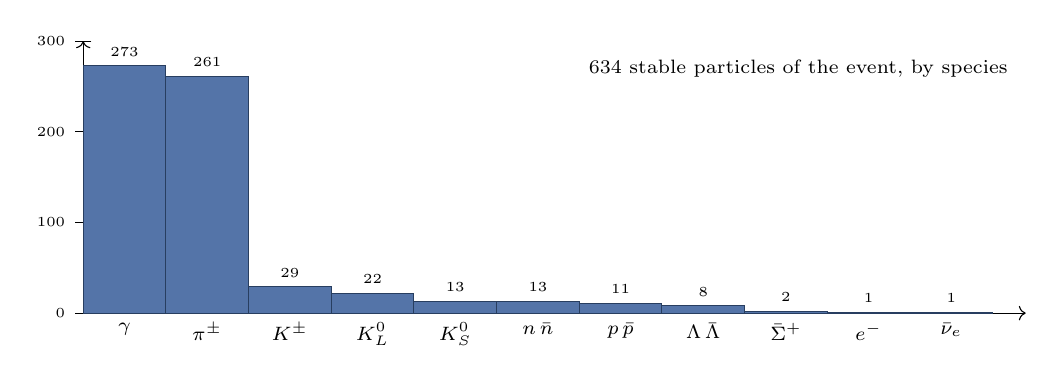
\begin{tikzpicture}[x=1.05cm, y=0.0115cm]
\draw[->] (0,0) -- (11.4,0);
\draw[->] (0,0) -- (0,300);
\foreach \y in {0,100,200,300} {\draw (0.1,\y) -- (-0.1,\y) node[left,font=\tiny] {\y};}
\histbar{0}{273} \histbar{1}{261} \histbar{2}{29} \histbar{3}{22} \histbar{4}{13} \histbar{5}{13}
\histbar{6}{11} \histbar{7}{8} \histbar{8}{2} \histbar{9}{1} \histbar{10}{1}
\foreach \x/\l in {0/$\gamma$, 1/$\pi^\pm$, 2/$K^\pm$, 3/$K^0_L$, 4/$K^0_S$, 5/$n\,\bar{n}$, 6/$p\,\bar{p}$, 7/$\Lambda\,\bar\Lambda$, 8/$\bar\Sigma^+$, 9/$e^-$, 10/$\bar\nu_e$}
  {\node[below, font=\scriptsize] at (\x+0.5,0) {\l};}
\node[font=\scriptsize, anchor=north east] at (11.3,290) {634 stable particles of the event, by species};
\end{tikzpicture}
\caption{The stable (status 1) particles of the event by species, from the FWLite count of
\code{test/06\_Decay/out/step1\_GEN\_06\_Decay.root} (companion, section 4). Photons, almost all from $\pi^0$
decays, and charged pions make 84\% of the final state by number.}
\label{fig:06_species}
\end{figure}

\begin{plainwords}[Why a jet is mostly photons and charged pions]
Strings fragment into pions in roughly equal numbers of $\pi^+$, $\pi^-$ and $\pi^0$ (here 261 charged pions
against 131 $\pi^0$, with a few from decays of heavier hadrons), plus a minority of kaons and baryons. The $\pi^0$
decays at once into two photons. So by the time Geant4 starts, a jet is a bundle of charged pions, which leave
tracks and then shower in the hadron calorimeter, and photons, which shower in the electromagnetic calorimeter.
That is the basis of particle-flow reconstruction and the reason the two calorimeters share the jet energy.
\end{plainwords}

\section{Ledger and display}
Table~\ref{tab:06_ledger} closes the ledger of the stage. Decays conserve energy and momentum, so the total energy
of the stable particles stays $13\,600.0\GeV$, the two proton energies. The scalar sum of \pt{} rises from
$505.7$ to $528.9\GeV$, because a decay shares the momentum of one particle among several that are not
collinear, and for the same reason energy migrates between the $\eta$ regions: the tracker region
$\abseta < 2.5$ gains $49\GeV$ and the region beyond $\abseta = 5.5$ loses $193\GeV$ as forward hadrons decay
into products spread over a wider range of $\eta$. The visible energy within $\abseta < 5.2$ grows from $5779$
to $5851\GeV$, while $95.5\GeV$ become invisible in the one neutrino: at this stage the only hole in the event
is the semileptonic $B^-$ decay.

\begin{table}[htbp]
\centering\small
\caption{Ledger of the decay stage: the stable (status 1) particles before (chapter~\ref{ch:05_Had},
\code{test/05\_Had/out/ledger\_05\_Had.txt}) and after the hadron decays (\code{test/06\_Decay/out/ledger\_06\_Decay.txt}).
$n$ is the number of particles, $E$ the energy and \pt{} the scalar sum of transverse momenta, in GeV.
The rows by region count every stable particle, the neutrino (at $\eta=-1.59$) included.}
\label{tab:06_ledger}
\begin{tabular}{@{}lrrrrrrrrr@{}}
\toprule
 & \multicolumn{3}{c}{before (05\_Had)} & \multicolumn{3}{c}{after (06\_Decay)} & \multicolumn{3}{c}{difference} \\
\cmidrule(lr){2-4}\cmidrule(lr){5-7}\cmidrule(lr){8-10}
 & $n$ & $E$ & \pt & $n$ & $E$ & \pt & $n$ & $E$ & \pt \\
\midrule
entries in \code{genParticles} & 1230 & & & 1846 & & & $+616$ & & \\
decayed (status 2)             & 0 & & & 302 & & & $+302$ & & \\
stable (status 1)              & 320 & 13600.0 & 505.7 & 634 & 13600.0 & 528.9 & $+314$ & 0.0 & $+23.2$ \\
\midrule
charged hadrons & 169 & 8863.8 & 355.0 & 303 & 7167.7 & 259.1 & $+134$ & $-1696.1$ & $-95.9$ \\
neutral hadrons & 151 & 4736.2 & 150.7 &  56 & 3449.9 &  84.7 & $-95$  & $-1286.3$ & $-66.0$ \\
photons         &   0 &    0.0 &   0.0 & 273 & 2875.9 & 142.7 & $+273$ & $+2875.9$ & $+142.7$ \\
electrons       &   0 &    0.0 &   0.0 &   1 &   10.9 &   5.0 & $+1$   & $+10.9$   & $+5.0$ \\
neutrinos       &   0 &    0.0 &   0.0 &   1 &   95.5 &  37.5 & $+1$   & $+95.5$   & $+37.5$ \\
\midrule
$\abseta < 2.5$ (tracker)        & 141 &  684.6 & 259.9 & 316 &  733.8 & 278.7 & $+175$ & $+49.2$  & $+18.8$ \\
$2.5 \le \abseta < 3.0$          &  30 &  196.8 &  24.6 &  55 &  193.1 &  24.6 & $+25$  & $-3.7$   & $0.0$ \\
$3.0 \le \abseta < 5.2$ (HF)     &  94 & 4897.9 & 192.4 & 189 & 5019.6 & 197.4 & $+95$  & $+121.7$ & $+5.0$ \\
$5.2 \le \abseta < 5.5$          &  15 &  810.7 &   7.9 &  16 &  836.4 &   7.8 & $+1$   & $+25.7$  & $-0.1$ \\
$\abseta \ge 5.5$ (not simulated) & 40 & 7010.1 &  20.9 &  58 & 6817.1 &  20.3 & $+18$  & $-193.0$ & $-0.6$ \\
\midrule
visible ($\abseta < 5.2$, no $\nu$) & 265 & 5779.2 & 476.9 & 559 & 5851.0 & 463.4 & $+294$ & $+71.8$ & $-13.5$ \\
invisible (neutrinos)               &   0 &    0.0 &   0.0 &   1 &   95.5 &  37.5 & $+1$   & $+95.5$ & $+37.5$ \\
\bottomrule
\end{tabular}
\end{table}

Figure~\ref{fig:06_display} is the $\eta$--$\phi$ display of the complete event. Compared with the stage-4
display of chapter~\ref{ch:05_Had}, where the $B^-$ and the $B^{*+}$ were two single large markers, the two
$b$ systems are now clusters of 9 (red) and 16 (blue) small markers around the same positions, $(\eta, \phi) =
(-1.57, -2.09)$ and $(-3.75, 1.01)$: the decay products of a $236\GeV$ and a $2421\GeV$ hadron stay within a
few tenths of a unit of their parent. This is the picture a jet algorithm will see in the next chapter. The
grey points are the 477 other decay products, the violet ones the 132 primary hadrons that did not decay; 38
particles beyond $\abseta = 6$ are drawn on the border.

\begin{figure}[htbp]
\centering
\includegraphics[width=\textwidth]{06_Decay/out/genPartAnalyzer_06_Decay_page-5.png}
\caption{The $\eta$--$\phi$ display of the complete generator event, stage 5 of
\code{test/06\_Decay/out/genPartAnalyzer\_06\_Decay.pdf} (page 5): the 634 stable particles, marker size growing with
\pt, coloured by origin. Red: the 9 stable decay products of the $B^-$; blue: the 16 of the $B^{*+}$; violet: the
primary hadrons left undecayed; grey: the decay products of the other hadrons. The magenta star is the vector sum
of the $b$ and $\bar{b}$ systems, $\pt = 20.3\GeV$.}
\label{fig:06_display}
\end{figure}

\FloatBarrier
\section{Open problems for Phase-2}
\paragraph{Which decay tables.}
This event is decayed with Pythia8's own tables: the GEN log prints ``no particle data has been changed from its
default value'', and the configuration has no \code{ExternalDecays} block. That is also what the Phase-2 release
validation does: the fragments it uses, \path{Configuration/Generator/python/TTbar_14TeV_TuneCP5_cfi.py} and
\path{MinBias_14TeV_pythia8_TuneCP5_cfi.py}, contain no external decayer either. The production fragments that
do use EvtGen do it through the \code{ExternalDecays} parameter set of the Pythia8 module, for example in
\path{Configuration/Generator/python/Hadronizer_TuneCP5_13TeV_aMCatNLO_FXFX_5f_max2j_max1p_LHE_pythia8_evtgen_cff.py}:
\code{EvtGen130} with \code{decay\_table} set to \path{GeneratorInterface/EvtGenInterface/data/DECAY_2010.DEC},
\code{particle\_property\_file} to \code{evt.pdl}, and empty \code{list\_forced\_decays} and \code{operates\_on\_particles}
(so EvtGen takes every species it knows, $b$ and $c$ hadrons among them). The $B$-physics fragments of the same
directory use \code{DECAY\_2014\_NOLONGLIFE.DEC} with \code{evt\_2014.pdl}, while the data package shipped with
the release (\path{cms-data/GeneratorInterface-EvtGenInterface}, V02-12-00, EvtGen~2.0.0) also carries
\code{DECAY\_2020.DEC} and \code{evt\_2020.pdl}, whose $B^-$ block still reads ``Updated to PDG 2008'' with
branching fractions marked PDG2014. Three generations of tables coexist in one release, and a 2010 table is
the default of the standard hadronizer fragment. The central Phase-2 Monte Carlo fragments are not part of the
release (they live in the production repository), so which table they use could not be established here;
what the release shows is that nothing selects a newer table by default, and that the Pythia8-only path of this
chapter is the one used for the Phase-2 relvals. For a $b$-jet study at the HL-LHC the semileptonic branching
fractions and the $D$ decay multiplicities, which set the neutrino energy and the track multiplicity in the jet,
are decided by this choice.

\paragraph{The lifetime boundary and the displaced vertices.}
\code{ParticleDecays:tau0Max = 10} (mm) in \path{Pythia8CommonSettings_cfi.py} is Pythia8's own default
(\code{ParticleDecays.xml}: \code{default="10."}); CMS only switches \code{limitTau0} on. The boundary has been
the same for Run~2, Run~3 and the Phase-2 relvals. It is a cut on the species, not on the vertex: in this event
the forward $B^+$ decays $117\mm$ from the primary vertex and its $\bar{D}^0$ at $258\mm$, inside the
acceptance window that Geant4 applies to generator vertices, \code{RDecLenCut = 2.9} and \code{LDecLenCut = 30.0} (cm)
in \path{SimG4Core/Application/python/g4SimHits_cfi.py}, but a $B$ hadron of a few TeV at larger $\eta$ would
not be. Everything above the boundary ($K^0_S$, $\Lambda$, $\Sigma$, $\Xi$, $\Omega$) decays in Geant4 with
Geant4's own branching fractions and kinematics, not Pythia8's; the generator-level $V^0$ content of a jet
is therefore split between two programs. For Phase-2 the vertex smearing changes module:
\path{IOMC/EventVertexGenerators/python/VtxSmearedRealisticHLLHC_cfi.py} (\code{HLLHCEvtVtxGenerator}, read from
the \code{SimBeamSpotHLLHCObjectsRcd} of the global tag), with the crab-cavity parameters of
\code{HLLHCVtxSmearingParameters} in \path{VtxSmearedParameters_cfi.py} (\code{CrossingAngleInurad = 510},
\code{BetaCrossingPlaneInm = 0.20}, \code{EprotonInGeV = 6500} in the base set, 7000 in the 14~TeV clone), which is
what the relval scenario \code{GenSimHLBeamSpot} of \path{Configuration/PyReleaseValidation/python/upgradeWorkflowComponents.py}
selects (\code{BeamSpot: DBrealisticHLLHC}, geometry \code{ExtendedRun4D110}, era \code{Phase2C17I13M9}). The
Phase-2 inner tracker that will resolve these vertices is described in the XML of
\path{Geometry/TrackerCommonData/data/PhaseII/}; its first-layer radius is not a python parameter and was not
extracted here.

\paragraph{The age of the common settings.}
\path{Pythia8CommonSettings_cfi.py} has eight lines and none of them is tune-specific:
\code{Tune:preferLHAPDF = 2} is the Pythia8 default (\code{Tunes.xml}) and does nothing;
\code{Main:timesAllowErrors = 10000} raises the number of flawed events Pythia8 may skip before it aborts from the
default 10, so that a sick configuration is not noticed; \code{Check:epTolErr = 0.01} loosens the
energy-momentum conservation check from the default $10^{-4}$ to 1\% of the collision energy, i.e. $136\GeV$ at
13.6~TeV; \code{SLHA:minMassSM = 1000} and \code{Beams:setProductionScalesFromLHEF = off} concern SUSY and
Les Houches input; \code{ParticleDecays:allowPhotonRadiation = on} adds QED radiation in decays to lepton pairs,
which the Pythia8 manual leaves off by default to avoid double counting with an external QED program such as
PHOTOS, which EvtGen runs. The block dates from the 2017 tune campaign and its physics content is the same in
CMSSW\_15\_0\_5. The tune itself is older than the beam energy: the fragment of the book imports
\path{Configuration/Generator/python/MCTunes2017/PythiaCP5Settings_cfi.py}, whose total and elastic cross
sections are the 13~TeV values, \code{SigmaTotal:sigmaTot = 100.309} and \code{sigmaEl = 21.89} (mb), while the
release also holds \path{MCTunesRun3ECM13p6TeV/PythiaCP5Settings_cfi.py} with 101.037 and 22.08~mb for
13.6~TeV; the 14~TeV fragments of the Phase-2 relvals (\code{TTbar\_14TeV\_TuneCP5\_cfi.py},
\code{MinBias\_14TeV\_pythia8\_TuneCP5\_cfi.py}) import the 2017 block as well, so no CP5 setting has been
re-derived for 14~TeV. These cross sections feed the MPI machinery (the log of this chapter computes
$\sigma_{\mathrm{ND}} = 55.42\mb$ from them) and, through the minimum-bias events of chapter~\ref{ch:08_PU},
the number of particles per pileup collision at PU~200.

\begin{plainwords}[What to take away]
The decays are the last step of the generator and the first place where the detector enters the physics choices:
a lifetime boundary of $10\mm$ decides who decays in Pythia8 and who in Geant4, the decay tables decide how often
a $b$ hadron produces a neutrino, and this event has one, $95.5\GeV$, 40\% of the $B^-$, which no later
stage will recover. Everything downstream, jets, pileup, Geant4, digitisation, reads the 634 stable particles of
this file.
\end{plainwords}

%% chapter_07_GenJet.tex -- chapter 07 of the JitJet book: the generator jets (process GENJET).
% Every number comes from test/07_GenJet/out/ (genJetAnalyzer_07_GenJet.log, ledger_07_GenJet.txt, the PNG pages) and
% from the FWLite extras listed in doc/chapter/chapter_07_GenJet.md, section 4.
\providecommand{\antikt}{anti-$k_{\mathrm{T}}$}
\providecommand{\dR}{\ensuremath{\Delta R}}

\chapter{07 -- GenJet: the 634 stable particles are clustered into \antikt{} jets}
\label{ch:07_GenJet}

\section{What this chapter is about}

Up to now the event has been a list of particles. A detector does not measure the $b$ quark of
chapter~\ref{ch:01_ME}, nor the $B^-$ meson of chapter~\ref{ch:05_Had}: it measures a spray of hadrons,
photons and leptons, and the only object that can be compared between theory and experiment is a
\emph{jet}, the sum of the particles inside a cone-like region defined by an algorithm. This chapter runs
that algorithm, \antikt{} as implemented in FastJet 3.4.1, on the 634 stable particles of the full generator
event and produces four collections of \emph{generator jets} (\code{reco::GenJet}): radius $R=0.4$ and
$R=0.8$, each once with all stable particles and once without the neutrinos. The clustering is done as a
separate \code{cmsRun} step, process \code{GENJET}, scheduled by \code{cmsDriver.py} as a \code{USER} step
with the sequence \code{genJetSequence} of \path{JitJetSW/Journey/python/genJet_cff.py}, with the jet
\pt{} threshold lowered to $3\GeV$ so that even the soft jets of the underlying event are visible.
The chapter explains the algorithm, the input selection, and reads the result for the one event: the $b$ jet
of $117.8\GeV$, the $\bar b$ jet of $115.9\GeV$, their balance, and why the $b$ jet is 28\,\% above
the quark it came from but 13\,\% below it once the neutrinos are left out.

\begin{plainwords}[A jet]
A jet is not a particle but a recipe: take the list of final-state particles, apply a clustering rule with a
radius parameter $R$, and call each resulting group a jet, with four-momentum equal to the vector sum of its
constituents. The same recipe applied to the stable particles of the generator gives a \emph{generator jet}
(this chapter), applied to the reconstructed particles of the detector gives a \emph{reconstructed jet}, and
the ratio of the two, the \emph{response}, is what the jet energy corrections (JEC) measure and undo. The
generator jet is therefore the reference of everything that follows in the detector chapters.
\end{plainwords}

\section{From the previous chapter}

The input is \path{test/06_Decay/out/step1_GEN_06_Decay.root}, the complete generator event of
chapter~\ref{ch:06_Decay}: 1846 entries in \code{genParticles}, of which 634 are stable (status~1) and carry
the $13\,600\GeV$ of the two protons, $528.9\GeV$ of scalar \pt{}.\footnote{All numbers of this chapter are
in \path{test/07_GenJet/out/genJetAnalyzer_07_GenJet.log} and \path{ledger_07_GenJet.txt}; the few extra
ones (the origin of the jet constituents, the unclustered particles by region) were read from the output ROOT
file with FWLite and are listed in the companion.} Nothing in that list changes here: the \code{GENJET} step
reads the file, adds the jet collections, and copies \code{genParticles} unchanged under its \code{GEN}
process name. The GEN step of chapter~\ref{ch:06_Decay} had in fact already clustered jets (the standard
\code{pgen} sequence contains \code{genJetMET}); those are dropped with
\code{--outputCommands "drop *\_ak4GenJets*\_*\_GEN,drop *\_ak8GenJets*\_*\_GEN"}, so that the output holds
exactly one set of jets, the one made and configured in this chapter.

The two objects to follow are the $b$ and $\bar b$ quarks. The hard-process $b$ (status~23,
$\pt=113.2\GeV$, $\eta=-1.44$) is pushed to $122.8\GeV$ by the recoil of the initial-state radiation
(status~44), radiates twice in the final-state shower (status~52: $106.0$, then $91.6\GeV$), receives its
primordial $k_{\mathrm{T}}$ (status~62, $91.7\GeV$) and is copied as the end of a colour string (status~71,
$\pt=91.74\GeV$, $\eta=-1.57$, $\phi=-2.08$). This status-71 copy is the quark the analyzer compares the
jets with. It fragments into the $B^-$ of $94.3\GeV$, which decays semileptonically,
$B^-\to D_0^{*0}\,e^-\,\bar\nu_e$, with the antineutrino carrying $37.5\GeV$ of \pt{} ($95.5\GeV$ of energy)
and nine stable decay products in all. The $\bar b$ goes from $113.2$ to $116.4\GeV$ (status~71,
$\eta=-3.75$, $\phi=1.01$), fragments into a $B^{*+}$ of $114.2\GeV$ and ends as 16 stable particles, none
of them a neutrino. At parton level the pair is already unbalanced: $|\vec p_{\mathrm T}(b)+\vec p_{\mathrm
T}(\bar b)|=25.1\GeV$ for the status-62 quarks and $20.3\GeV$ for the two $B$ hadrons, against $0$ for the
hard process. Jets exist to recover what the radiation took away.

\section{The numbers of the event}

\begin{plainwords}[The \antikt{} algorithm]
FastJet computes for every pair of particles $d_{ij}=\min(1/p_{\mathrm{T}i}^2,\,1/p_{\mathrm{T}j}^2)\,
\Delta R_{ij}^2/R^2$ with $\Delta R_{ij}^2=(\eta_i-\eta_j)^2+(\phi_i-\phi_j)^2$, and for every particle
$d_{iB}=1/p_{\mathrm{T}i}^2$ (the distance to the beam). The smallest of all these numbers decides: if it is a
$d_{ij}$, $i$ and $j$ are merged (four-momenta added) and the list is recomputed; if it is a $d_{iB}$, $i$ is
declared a jet and removed. The inverse powers of \pt{} make the hardest particle the first to act: it
swallows everything within \dR$<R$ around it before any soft particle can merge with another soft one, so a
hard jet is a circle of radius $R$ around its axis, as in the display, and the soft background does not move
its axis. Two properties make the definition usable in perturbative QCD: a soft particle added anywhere does
not change the hard jets (\emph{infrared safety}), and a particle split into two collinear ones gives the
same jets (\emph{collinear safety}); a cone algorithm seeded on the hardest particle has neither. The jet
\pt{} is the \pt{} of the vector sum, slightly smaller than the scalar sum of its constituents.
\end{plainwords}

\textbf{The producer and its input.} Each collection is one \code{FastjetJetProducer} module
(\path{RecoJets/JetProducers/python/ak4GenJets_cfi.py}: \code{jetAlgorithm} \code{"AntiKt"}, \code{rParam} 0.4;
\path{ak8GenJets_cfi.py} clones it with \code{rParam} 0.8) that reads the parameter set
\code{GenJetParameters} (\path{GenJetParameters_cfi.py}): \code{jetType} \code{'GenJet'},
\code{jetPtMin} \code{3.0}, \code{inputEtMin} \code{0.0}, \code{inputEMin} \code{0.0}, no area, no $\rho$ subtraction, a
deterministic FastJet seed. \code{jetPtMin} is the only threshold: jets below it are not written. The script
sets it explicitly to the same $3\GeV$ for the four producers, through \code{--customise\_commands}, so that it
can be changed with \code{JETPTMIN}. The input is not \code{genParticles} itself but a selection made by
\code{InputGenJetsParticleSelector} (\path{RecoJets/Configuration/python/GenJetParticles_cff.py}): it keeps
every status-1 particle except those whose $|\mathrm{pdgId}|$ is in \code{ignoreParticleIDs}. For
\code{genParticlesForJets} that list contains only hypothetical invisible particles: 1000022 (the lightest
neutralino), 1000012/14/16 and 2000012/14/16 (left- and right-handed sneutrinos), 1000039 (gravitino),
5100039 (Kaluza--Klein graviton), 4000012/14/16 (excited neutrinos), 9900012/14/16 (heavy Majorana
neutrinos) and 39 (graviton). None of them occurs in a Pythia8 \bbbar{} event, so all 634 stable particles
are offered to the clustering. \code{genParticlesForJetsNoNu} adds 12, 14, 16, the three neutrinos: 633
particles. The other switches are off: \code{excludeResonances = False} (no removal of $W/Z/H$ decay
products), \code{tausAsJets = False}, \code{partonicFinalState = False}.

\begin{table}[htb]
\centering\small
\caption{The $b$ and $\bar b$ jets in the three collections drawn (\code{genJetAnalyzer\_07\_GenJet.log}).
The quark is the status-71 copy ($\pt=91.74$ and $116.36\GeV$); \dR{} is the distance between jet axis
and quark; the net \pt{} and $\Delta\phi$ are those of the pair; $m_{jj}$ is read from the page header
(\code{genJetAnalyzer\_07\_GenJet\_page-6/7/8.png}).}
\label{tab:07_bjets}
\begin{tabular}{llrrrrrrr}
\toprule
collection & jet & \pt{} [GeV] & $\eta$ & $\phi$ & $n$ & \dR{} & $\pt^{\mathrm{jet}}/\pt^{q}$ & mass [GeV] \\
\midrule
\code{ak4GenJets}     & $b$       & 117.79 & $-1.59$ & $-2.08$ & 24 & 0.019 & 1.284 & 16.7 \\
                      & $\bar b$  & 115.94 & $-3.75$ & $1.01$  & 18 & 0.004 & 0.996 & 7.3 \\
                      & pair      & \multicolumn{7}{l}{net $\pt=6.06\GeV$, $\Delta\phi=3.09$, $\Sigma\pt=233.7\GeV$, $m_{jj}=386.8\GeV$} \\
\addlinespace
\code{ak4GenJetsNoNu} & $b$       & 79.82  & $-1.59$ & $-2.08$ & 22 & 0.017 & 0.870 & 13.4 \\
                      & $\bar b$  & 115.94 & $-3.75$ & $1.01$  & 18 & 0.004 & 0.996 & 7.3 \\
                      & pair      & \multicolumn{7}{l}{net $\pt=36.53\GeV$, $\Delta\phi=3.09$, $\Sigma\pt=195.8\GeV$, $m_{jj}=319.7\GeV$} \\
\addlinespace
\code{ak8GenJets}     & $b$       & 141.10 & $-1.65$ & $-2.05$ & 55 & 0.088 & 1.538 & 47.3 \\
                      & $\bar b$  & 121.01 & $-3.75$ & $0.99$  & 32 & 0.022 & 1.040 & 19.0 \\
                      & pair      & \multicolumn{7}{l}{net $\pt=24.03\GeV$, $\Delta\phi=3.04$, $\Sigma\pt=262.1\GeV$, $m_{jj}=439.5\GeV$} \\
\bottomrule
\end{tabular}
\end{table}

\textbf{The $b$ jet and its response.} With $R=0.4$ the $b$ quark is matched to jet~[0], $\pt=117.79\GeV$,
24 constituents, axis $0.019$ away from the quark direction. Its response with respect to the status-71 quark
is $117.79/91.74=1.284$. A response above one is not an excess of energy, it is the bookkeeping of the
shower: the quark used as reference has already radiated. Measured against the hard-process $b$ of
$113.2\GeV$ the same jet has a response of $1.04$. The constituents tell where the \pt{} comes from. Nine of
the 24 are the decay products of the $B^-$ and carry $94.3\GeV$ (the neutrino alone $37.5\GeV$). Seven more,
$17.5\GeV$, are hadrons from the same colour string as the $b$ quark, the string formed by the $b$, three
gluons and an $\bar s$ quark of the shower: this is the radiated energy coming back. The remaining eight,
$6.4\GeV$, come from other strings, those of the multiparton interactions and of the beam remnants: the
underlying event that happens to fall inside the circle. The $\bar b$ jet at $\eta=-3.75$ is cleaner: 16 of
its 18 constituents are the $B^{*+}$ decay products ($114.2\GeV$), one $K^-$ of $1.6\GeV$ comes from the
$\bar b$ string and one photon of $0.15\GeV$ from elsewhere; response $0.996$.

\begin{plainwords}[Why 1.28 with neutrinos and 0.87 without]
The $B^-$ decayed semileptonically and its antineutrino carries $37.5\GeV$ of the jet's $117.8\GeV$.
\code{ak4GenJetsNoNu} drops the three neutrino species before clustering: the $b$ jet becomes
$79.82\GeV$ (response $0.870$), with 22 constituents instead of 24 because, with the neutrino gone, the axis
moved and a $0.5\GeV$ pion at the edge now belongs to the neighbouring jet~[4] ($11.89\to12.40\GeV$, 11 to 12
constituents). The $\bar b$ jet, without a neutrino, is identical in both collections. The dijet balance
follows: with neutrinos the pair has a net \pt{} of $6.1\GeV$ and $\Delta\phi=3.09$, the best balance of the
whole journey ($25.1\GeV$ at quark level); without, $36.5\GeV$ is missing in the direction of the $b$ jet,
exactly the signature a detector would call missing transverse energy. Which of the two is the right reference
depends on the question: the NoNu jets are what a calorimeter can see at best and are the reference of the
jet energy corrections; the full jets are the parton-level truth.
\end{plainwords}

\textbf{$R=0.4$ against $R=0.8$.} Doubling the radius quadruples the area. The $b$ jet of \code{ak8GenJets}
has $141.10\GeV$ and 55 constituents, response $1.538$ (1.25 against the hard-process quark), mass
$47.3\GeV$ instead of $16.7$; its axis is $0.088$ from the quark. The additions are $19.8\GeV$ of further
hadrons of the $b$ string (8 particles, in all 17 of the 55 constituents and $114.2\GeV$ belong to the $b$
string) and $28.5\GeV$ from 38 particles of other strings. The $\bar b$ jet gains $5.1\GeV$ ($121.01\GeV$,
32 constituents). The pair is now less balanced, net $\pt=24.0\GeV$, $\Delta\phi=3.04$: the large cone
collects the underlying event unevenly. In \code{ak8GenJets} 488 of the 634 stable particles are in a jet and
28 jets are found; jets [2] to [7] have $10$ to $29\GeV$ and 17 to 37 constituents each, merged soft activity
that \code{ak4GenJets} splits into several $5$ to $14\GeV$ jets. The small radius is the one used for most
of CMS physics, with the underlying event and (later) the pileup as the price of a large one.

\textbf{The other jets and the unclustered particles.} \code{ak4GenJets} finds 27 jets above $3\GeV$. Besides
the two $b$ jets, jets~[2] to [5] ($13.8$, $13.3$, $11.9$, $11.4\GeV$, 10 to 12 constituents) are the
hadronised radiation and multiparton interactions of chapters~\ref{ch:02_PS} and \ref{ch:04_MPI}; the
remaining 21 have $3.2$ to $7.1\GeV$. In all, 239 of the 634 stable particles are inside a jet and the jets
sum to $382.8\GeV$ of \pt{}. The 395 unclustered particles carry $144.6\GeV$ of scalar \pt{}: 298 of them are
below $0.5\GeV$, 78 between $0.5$ and $1\GeV$, only two above $2\GeV$ (the hardest $2.3\GeV$), and 38 sit
beyond $|\eta|=6$, on the border of the display. They carry, however, $9615\GeV$ of energy, almost all of it
beam remnants along the beam pipe, which is why the jet energy ($3985\GeV$) is a small part of the event
energy. By region, the 27 \code{ak4GenJets} are 17 at $\abseta<2.5$ ($217.9\GeV$), 4 at $2.5<\abseta<3.0$
($18.5\GeV$) and 6 at $3.0<\abseta<5.2$ ($146.3\GeV$, among them the $\bar b$ jet); none is beyond $5.2$,
while \code{ak8GenJets} has three jets there ($16.1\GeV$, up to $\eta=6.1$). Generator jets have no $\eta$
limit; the detector will set one.

\section{Ledger and display}

\begin{table}[H]
\centering\small
\caption{Ledger of the GenJet stage (\code{ledger\_07\_GenJet.txt}; the unclustered and per-region lines from
the FWLite extras of the companion). The stage adds nothing to and removes nothing from the event: it
partitions the 634 stable particles into jets and a remainder. The jet \pt{} is the vector sum per jet, the
particle sums are scalar.}
\label{tab:07_ledger}
\begin{tabular}{lrrrrrr}
\toprule
& \multicolumn{3}{c}{before: stable particles} & \multicolumn{3}{c}{after: \code{ak4GenJets}} \\
\cmidrule(lr){2-4}\cmidrule(lr){5-7}
 & $n$ & $E$ [GeV] & \pt{} [GeV] & jets & $n_{\mathrm{const}}$ & $\Sigma\pt$ [GeV] \\
\midrule
all, in a jet           & 634 & 13600.0 & 528.9 & 27 & 239 & 382.8 \\
all, not in a jet       &     &         &       & -- & 395 & 144.6 \\
$\abseta<2.5$           & 316 & 733.8   & 278.7 & 17 &     & 217.9 \\
$2.5<\abseta<3.0$       & 55  & 193.1   & 24.6  & 4  &     & 18.5 \\
$3.0<\abseta<5.2$       & 189 & 5019.6  & 197.4 & 6  &     & 146.3 \\
$\abseta>5.2$           & 74  & 7653.5  & 28.1  & 0  &     & 0 \\
neutrinos               & 1   & 95.5    & 37.5  & \multicolumn{3}{l}{in \code{ak4GenJets}, not in \code{NoNu}} \\
\midrule
\code{ak4GenJets}       &     &         &       & 27 & 239 & 382.8 \ ($\Sigma E=3985.2$) \\
\code{ak4GenJetsNoNu}   &     &         &       & 27 & 238 & 345.3 \ ($\Sigma E=3889.7$) \\
\code{ak8GenJets}       &     &         &       & 28 & 488 & 473.1 \ ($\Sigma E=7613.4$) \\
\bottomrule
\end{tabular}

\medskip
\begin{tabular}{lrrrrrr}
\toprule
$b+\bar b$ pair [GeV] & hard process & status 62 & $B$ hadrons & \code{ak4GenJets} & \code{NoNu} & \code{ak8GenJets} \\
\midrule
scalar sum \pt{} & 226.4 & 208.1 & 208.5 & 233.7 & 195.8 & 262.1 \\
net \pt{}        & 0.0   & 25.1  & 20.3  & 6.1   & 36.5  & 24.0 \\
\bottomrule
\end{tabular}
\end{table}

\begin{figure}[H]
\centering
\includegraphics[width=0.8\textwidth]{07_GenJet/out/genJetAnalyzer_07_GenJet_page-6.png}
\caption{\code{ak4GenJets}: the 27 \antikt{} $R=0.4$ jets with $\pt>3\GeV$ of the event, over the 634 stable
particles (marker size $\sim\log\pt$). The $b$ jet [0] ($117.8\GeV$, red) and the $\bar b$ jet [1]
($115.9\GeV$, blue) are matched to the status-71 quarks (stars). Pages 1--5 of the same PDF are the five
generator stages of chapters~\ref{ch:01_ME}--\ref{ch:06_Decay}.
(\code{test/07\_GenJet/out/genJetAnalyzer\_07\_GenJet\_page-6.png})}
\label{fig:07_ak4}
\end{figure}

Figure~\ref{fig:07_ak4} is the $\eta$--$\phi$ display of the event at this stage: every jet is a circle of
radius $R$ around its axis, its constituents in the jet colour, the unclustered stable particles in grey, the
$b$ and $\bar b$ jets in red and blue with the quark direction as an open star. The two $b$ jets are
back-to-back in $\phi$ ($\Delta\phi=3.09$) and far apart in $\eta$ ($-1.59$ and $-3.75$), the picture of a
$\qqbar\to\bbbar$ event with a very asymmetric $x_1=0.39$, $x_2=0.0022$ of chapter~\ref{ch:01_ME}. The
circles of the 25 other jets, mostly in the central region, are the hadronised shower and MPI. The grey
particles between the circles and the 38 crosses on the $|\eta|=6$ border are the beam remnants.
Figure~\ref{fig:07_nonu_ak8} shows the same event without neutrinos (the $b$ jet shrinks to $79.8\GeV$,
nothing else moves) and with $R=0.8$ (the circles overlap, 488 particles are clustered, the display fills
up).


\begin{figure}[htb]
\centering
\begin{subfigure}[t]{0.495\textwidth}
\includegraphics[width=\textwidth]{07_GenJet/out/genJetAnalyzer_07_GenJet_page-7.png}
\caption{\code{ak4GenJetsNoNu}: without the neutrino the $b$ jet is $79.8\GeV$.}
\end{subfigure}\hfill
\begin{subfigure}[t]{0.495\textwidth}
\includegraphics[width=\textwidth]{07_GenJet/out/genJetAnalyzer_07_GenJet_page-8.png}
\caption{\code{ak8GenJets}: $R=0.8$, the $b$ jet is $141.1\GeV$ with 55 constituents.}
\end{subfigure}
\caption{The same event in the two other collections
(\code{genJetAnalyzer\_07\_GenJet\_page-7.png}, \code{page-8.png}).}
\label{fig:07_nonu_ak8}
\end{figure}

\FloatBarrier
\section{Open problems for Phase-2}

The generator jets are the reference of the jet energy scale, so what is frozen here is frozen for the whole
HL-LHC programme. A look into \code{CMSSW\_15\_0\_5} gives the following.

\textbf{The definitions have not moved since Run 2.} \path{RecoJets/JetProducers/python/GenJetParameters_cfi.py}
sets \code{jetPtMin} \code{3.0}, \code{inputEtMin} \code{0.0}, \code{inputEMin} \code{0.0}, \code{doAreaFastjet}
\code{False}, \code{doRhoFastjet} \code{False}; \path{ak4GenJets_cfi.py} and \path{ak8GenJets_cfi.py} fix \code{rParam} to 0.4
and 0.8. No file in \path{RecoJets/Configuration/python} or \path{RecoJets/JetProducers/python} carries a
\code{phase2} era modifier for the generator jets (the only \code{phase2} strings in \code{RecoJets} are the
heavy-ion event content, \path{RecoJets_EventContent_cff.py}, and \path{CaloTowersES_cfi.py}); the Phase-2
GEN step of \path{doc/tmp/Gen4Phase2.md} runs byte-identical producers. The thresholds that matter
downstream are also unchanged: miniAOD keeps \code{slimmedGenJets} from \code{ak4GenJetsNoNu} without a
cut and \code{slimmedGenJetsAK8} from \code{ak8GenJetsNoNu} with \code{pt > 80}
(\path{PhysicsTools/PatAlgos/python/slimming/slimmedGenJets_cfi.py}); nanoAOD writes \code{GenJet} with
\code{pt > 10} and \code{GenJetAK8} with \code{pt > 100} (\path{PhysicsTools/NanoAOD/python/jetMC_cff.py}).
Note that the compiled default of \code{jetPtMin} in \code{VirtualJetProducer::fillDescriptions} is $5\GeV$
while the \code{cfi} says $3\GeV$: the \code{cfi} wins, but a module built without it would cut differently.
None of this is wrong for Phase-2, but none of it was revisited for it either.

\textbf{The exclusion lists are the 2007 lists.} The file
\path{RecoJets/Configuration/python/GenJetParticles_cff.py} is headed ``ShR 27 Mar 07'' and its \code{ignoreParticleIDs} are the invisible BSM particles listed above; the
only later additions are the \code{NoNu} (12, 14, 16) and \code{NoMuNoNu} (12, 13, 14, 16) clones. There is
no pileup-robust generator-jet definition and there need not be one: \code{genParticles} holds only the
signal collision, so a generator jet is pileup-free by construction (chapter~\ref{ch:08_PU} shows what happens
when the pileup particles are added to the clustering on purpose). The pileup robustness is entirely on the
reconstruction side, and that side has been retuned for Phase-2: \path{CommonTools/PileupAlgos/python/Puppi_cff.py}
modifies \code{puppi} under \code{phase2\_common} with \code{EtaMinUseDeltaZ = 4.0}, \code{DeltaZCut = 0.1},
\code{MinNeutralPt = 0.2} up to $\abseta=3.5$ and $2.0$ beyond, with the $\eta$ regions $0$--$2.5$,
$2.5$--$3.5$, $3.5$--$10$. The reference against which that tuning is judged remains the unchanged
\code{ak4GenJetsNoNu}. One open point for a $b$-rich analysis is the one visible in this event: the
\code{NoNu} reference removes the $37.5\GeV$ neutrino and makes the $b$ jet response $0.87$, so the flavour
dependence of the corrections, measured against this reference, is as large at the HL-LHC as it is now.

\textbf{The $\eta$ reach.} Generator jets have no $\eta$ cut; in this event \code{ak4GenJets} reach
$\eta=-4.70$ and \code{ak8GenJets} $\eta=6.12$. The Run-3 detector of this book sees jets up to
$\abseta\approx5.2$ with the HF, with the region $2.5$--$3.0$ covered by calorimeters only; the Phase-2 layout
in the release puts the tracker to $\abseta=4.0$ (the \code{EtaMinUseDeltaZ = 4.0} of Puppi above), the
HGCal at $1.5<\abseta<3.0$ and the HF at $3.0<\abseta<5.5$, as spelled out by the region boundaries of the
Phase-2 Level-1 particle flow, \path{L1Trigger/Phase2L1ParticleFlow/python/l1ctLayer1_cff.py}
(\code{etaBoundaries = (-1.5, 1.5)}, \code{(1.5, 3.0)}, \code{(3.0, 5.5)}). In the ledger of this event the
$2.5<\abseta<3.0$ region holds 4 \code{ak4GenJets} ($18.5\GeV$) and $3.0<\abseta<5.2$ holds 6
($146.3\GeV$, the $\bar b$ jet among them): with the HGCal and the extended tracker the $\bar b$ jet of
this event, at $\eta=-3.75$, is still an HF jet, and its $B^{*+}$ decay products at $\abseta>3$ are still
untracked. Whether the generator-jet validation follows the new boundaries could not be established:
\path{Validation/RecoJets/python} contains no \code{phase2} modifier.

\textbf{The jet energy corrections of Phase-2.} The chain that turns a reconstructed jet into a
generator-jet-like one is a sequence of \code{JetCorrectorParametersCollection} payloads in the global tag.
For the Phase-2 tag of this release, \path{auto:phase2_realistic} $=$ \path{150X_mcRun4_realistic_v1}
(\path{Configuration/AlCa/python/autoCond.py}), \code{conddb list} gives: \code{AK4PF}, \code{AK8PF} and
\code{AK8PFchs} from \path{PhaseIIFall17_V5_MC}, a 2017 Phase-2 study; \code{AK4PFPuppi},
\code{AK4PFchs} and \code{AK8PFPuppi}, the collections actually used offline, from
\path{Winter22Run3_V1_MC}, i.e.\ a Run-3 payload applied to the Phase-2 detector; only the HLT one,
\code{AK4PFPuppiHLT}, is recent and Phase-2 (\path{Phase2Spring23ticlv4_MC_v1}). The jet resolution
payloads of the same tag are all \path{JR_Spring16_25nsV6_MC}, from 2016. For comparison the 2024 tag of
this book, \path{150X_mcRun3_2024_realistic_v2}, has \path{Winter24_AK4PFPuppi_offline_v1} and
\path{JR_Summer19UL18_JRV2}. All of them take \code{ak4GenJetsNoNu} (or \code{ak8GenJetsNoNu}) matched
to the reconstructed jet as the truth: the generator jets of this chapter, with their 2007 input list and
$3\GeV$ threshold, are the reference of the HL-LHC jet energy scale until a Phase-2 payload is derived, and
they will have to serve at PU 200 and $14\TeV$ without having been changed for either. What could not be
established from the release: the $\eta$ binning of the Phase-2 payloads (the files live only in the
database, \path{CondFormats/JetMETObjects/data} holds no Run-3 or Phase-2 text file) and whether the matching
radius and \pt{} thresholds used to derive them will be adjusted for the HGCal granularity.

%\chapter{08 -- Pileup: the other 68 collisions of the bunch crossing, at generator level}
\label{ch:08_PU}

\section{What this chapter is about}

In 2025, the year of the release the book runs, a bunch crossing at CMS held on average some 60 inelastic
proton--proton collisions (64 in the 2025 profile of the release; the book takes 60). One of them is the \bbbar{} event the book follows; the others are \emph{pileup}, ordinary inelastic collisions
that happen to sit in the same 25\,ns window and that the detector cannot tell apart from the signal. Before
anything is simulated in the detector these collisions have to be generated, and this chapter does that
alone: it runs Pythia8 with the minimum-bias fragment of the release, \code{MinBias\_14TeV\_pythia8\_TuneCP5\_cfi},
at the $13.6\TeV$ of the signal, 250 times, and asks what an inelastic collision is (non-diffractive or
diffractive, how many parton pairs interact, how many hadrons come out, where the vertex is in space and
time). The 250 collisions are the generator-level \emph{pileup library} of the book; one of them is drawn
with the five generator pages of chapters 01--06.

The chapter then puts the pileup where it belongs, on top of the signal, still without a detector: the
stable particles of the 68 library collisions that will share the bunch crossing of our event in
chapters~\ref{ch:10_SIM} and \ref{ch:11_DIGI} are added to the 634 stable particles of chapter~\ref{ch:07_GenJet},
and the anti-$k_{\mathrm{T}}$ clustering is run again on the sum. The $b$ jet goes from 117.8 to
$150.9\GeV$ and 266 jets appear where there were 27: this is what pileup does to a jet before any detector
effect, and the number every pileup correction of the reconstruction will later try to undo.

\begin{plainwords}[Minimum bias]
The name is historical: a ``minimum-bias trigger'' was the loosest trigger an experiment could run, firing
on essentially any inelastic collision. A minimum-bias \emph{sample} is thus a sample of ordinary inelastic
collisions, with nothing selected and nothing enriched: the inelastic cross section itself, sampled in its
natural proportions, with no \ptHat{} cut and no filter. That is exactly what the other collisions of a bunch
crossing are, so a minimum-bias generator run is the raw material of pileup. In Pythia8 it is one switch,
\code{SoftQCD:inelastic = on}.
\end{plainwords}

\section{From the previous chapter}

Chapter~\ref{ch:07_GenJet} left the signal as a GEN file with its jets
(\path{test/07_GenJet/out/step2_GENJET_07_GenJet.root}): 1846 generator particles, 634 of them stable,
and 27 anti-$k_{\mathrm{T}}$ $R=0.4$ jets above $3\GeV$, the $b$ jet at $\pt=117.8\GeV$ ($\eta=-1.59$) and
the $\bar b$ jet at $115.9\GeV$ ($\eta=-3.75$). Nothing of it is rerun here (sample 8a); its jets alone are
the pages of chapter~\ref{ch:07_GenJet}, and \code{genJetAnalyzer\_08\_PU.pdf} holds the overlay.

The new ingredient is the library (sample 8b): 250 minimum-bias collisions generated by the GEN step of the
signal (vertex smearing from the database, energy) but with its own random seeds, so that its vertices are not
those of the signal. It is the first job of the book with the 2025 settings of the release, global tag
\code{auto:phase1\_2025\_realistic} and era \code{Run3\_2025}, as all the CMS chapters 08--13,
where the generator chapters 01--07 keep those of 2024; at generator level the two are the
same (section~\ref{sec:08_numbers}). The overlay (sample 8a+8b) takes library events 72 to 139 (\code{SKIP = 71}, \code{NPU = 68} in
\path{test/common/jitjet_common.sh}). Why these: the \code{MixingModule} of chapter~\ref{ch:10_SIM} (seed
12345, a Poisson draw with mean 60 per bunch crossing) reads the library in sequence, bunch crossing by bunch
crossing, early crossings first; for this signal event it draws 71 collisions for bunch crossing $-1$
(library events 1--71), 68 for bunch crossing 0 (events 72--139) and 54 for bunch crossing $+1$ (events
140--193). Library events 72--139 are therefore the in-time collisions of \emph{this} signal event, the same
ones, collision by collision, that the detector simulation will see in the same 25\,ns as the signal;
chapter~\ref{ch:10_SIM} checks its draw against them and chapter~\ref{ch:11_DIGI} replays it with the
playback of the \code{MixingModule}. Only in-time
collisions matter at generator level: a list of particles has no time axis, so the early and late crossings
can only act through the time response of the detector.

\section{The numbers of the event}
\label{sec:08_numbers}

\paragraph{The inelastic cross section.} Pythia8 prints, at the initialisation of the job, what it is
about to generate (table~\ref{tab:xsec}): ``We collide p+ with p+ at a CM energy of 1.360e+04 GeV'' and the
five subprocesses of \code{SoftQCD:inelastic} with their cross sections.\footnote{All numbers of this
section are from \code{test/08\_PU/out/step1\_GEN\_MinBias\_08\_PU.log} (the Pythia8 banner and statistics),
\code{gencheck\_08\_PU.log} and \code{genstats\_08\_PU.txt} (the catalogue of \code{common/minBiasGenStats.py}).}
The total and elastic cross sections are not computed: the tune CP5 fixes them
(\code{SigmaTotal:mode = 0}, \code{sigmaTot = 100.309}, \code{sigmaEl = 21.89} mb, in
\code{Configuration/Generator/python/MCTunes2017/PythiaCP5Settings\_cfi.py}), so that
$\sigma_{\mathrm{inel}} = 100.31 - 21.89 = 78.42\mb$ whatever the energy; the diffractive pieces come from
Pythia's own parametrisation and the non-diffractive cross section is the remainder. Pythia chooses the
process of every event in proportion to these numbers: 183 ND, 45 SD, 19 DD and 3 CD in the 250 events,
against 176.7, 41.0, 28.2 and 4.1 expected (the DD deficit is 1.7 standard deviations; the rest is within
one). The \code{GenXsecAnalyzer} at the end of the log reports the same $7.842\times10^{10}$\,pb with a filter
efficiency of $250/250$; the \code{crossSection = 71.39e+09} written in the fragment is old metadata that
nothing uses.

\begin{table}[htbp]
\centering\small\setlength{\tabcolsep}{4pt}
\caption{The inelastic collision in Pythia8 at $13.6\TeV$ with the tune CP5: the cross sections of the
``PYTHIA Process Initialization'' table of \code{step1\_GEN\_MinBias\_08\_PU.log}, and how many of the 250
collisions came out of each process (``Event and Cross Section Statistics'').}
\label{tab:xsec}
\begin{tabular}{llrrrr}
\toprule
process & code & $\sigma$ [mb] & share & expected of 250 & generated \\
\midrule
non-diffractive (ND), $pp\to X$        & 101       & 55.42 & 70.7\,\% & 176.7 & 183 \\
single diffractive (SD), $pp\to pX, Xp$ & 103 + 104 & $2\times6.43$ & 16.4\,\% & 41.0 & 45 (27 + 18) \\
double diffractive (DD), $pp\to XX$    & 105       & 8.85  & 11.3\,\% & 28.2 & 19 \\
central diffractive (CD), $pp\to pXp$  & 106       & 1.29  & 1.6\,\%  & 4.1 & 3 \\
\midrule
inelastic (\code{SoftQCD:inelastic})   & sum       & 78.42 & 100\,\%  & 250 & 250 \\
elastic, $pp\to pp$ (not generated)    & 102       & 21.89 & -- & -- & -- \\
total (fixed by CP5)                   &           & 100.31 & & & \\
\bottomrule
\end{tabular}
\end{table}

\begin{plainwords}[Four ways for two protons to collide inelastically]
Picture the two protons as bags of quarks and gluons. In a \emph{non-diffractive} collision the bags tear
open and their contents interact directly; the whole rapidity range fills with particles. In a
\emph{diffractive} collision the protons exchange something colourless (a ``Pomeron''), so that one of them
(SD) or both (DD) keep their identity or dissolve into a low-mass bunch of hadrons flying on along the beam,
and a gap with no particles separates the two sides. In a \emph{central-diffractive} collision both protons
survive and only a small system is created in the middle. The LHC does not pick: it makes all four in the
proportions of table~\ref{tab:xsec}, and so does the generator.
\end{plainwords}

\paragraph{Multiparton interactions set the size of a collision.} A non-diffractive collision has no hard
process to speak of; its multiplicity comes from the multiparton interactions of chapter~\ref{ch:04_MPI}.
The log shows the regularisation scale of the MPI cross section, $\pt^0 = 1.41\times(13.6/7)^{0.03344} =
1.44\GeV$ (\code{pT0Ref} and \code{ecmPow} of CP5), and ``pT0 = 1.44 gives sigmaInteraction = 492.18 mb'':
the integrated parton--parton cross section above the cut-off is nine times the non-diffractive cross
section of $55.42\mb$, so on average nine parton pairs interact per ND collision. The catalogue confirms it:
counting the hardest scattering plus one interaction per pair of status-31 partons, the 183 ND collisions
have between 1 and 39 interactions, mean 9.0, and the number of stable particles follows them almost
linearly, from 85 for one interaction (44 collisions) to 723 for 39 (the largest collision of the file,
event 247). The diffractive collisions have on average 1.2 to 2.0 interactions and are nearly empty for the central
detector: 70 stable particles and 7 central ones for SD, 57 and 2 for DD, 35 and 2 for CD, against 241 and
27 for ND (table~\ref{tab:cat}).

\begin{table}[htbp]
\centering\small
\caption{The 250 minimum-bias collisions at generator level (\code{genstats\_08\_PU.txt}): per collision,
the stable particles (HepMC status 1), the charged ones, the ``central'' ones ($\abseta<2.5$,
$\pt>0.5\GeV$), those beyond $\abseta=5.5$ where no CMS subdetector is, the hardest particle, the scalar
sum of \pt{}, the anti-$k_{\mathrm{T}}$ $R=0.4$ jets above $10\GeV$, and the smeared vertex. By process:
183 ND / 45 SD / 19 DD / 3 CD collisions with on average 241 / 70 / 57 / 35 stable and 27 / 7 / 2 / 2
central particles.}
\label{tab:cat}
\begin{tabular}{lrrrr}
\toprule
per collision & mean & median & min & max \\
\midrule
parton--parton interactions (1 + MPI) & 7.0 & 3 & 1 & 39 \\
stable particles & 193.8 & 132 & 3 & 723 \\
charged stable particles & 89.0 & 59 & 2 & 320 \\
central ($\abseta<2.5$, $\pt>0.5\GeV$) & 21.2 & 9.5 & 0 & 126 \\
beyond $\abseta=5.5$ & 38.9 & 36.5 & 3 & 93 \\
\pt{} of the hardest particle [GeV] & 2.20 & 1.81 & 0.23 & 8.08 \\
scalar sum of \pt{} [GeV] & 79.2 & 44.7 & 0.5 & 376.1 \\
jets above $10\GeV$ & 0.15 & 0 & 0 & 3 \\
vertex $z$ [cm] (r.m.s.\ 3.56) & 0.08 & $-0.05$ & $-9.5$ & 10.1 \\
vertex $t$ [ns] (r.m.s.\ 0.122) & $-0.007$ & $-0.015$ & $-0.39$ & 0.37 \\
\bottomrule
\end{tabular}
\end{table}

\paragraph{What a minimum-bias collision is made of.} Of the 48\,437 stable particles of the 250
collisions, 45.9\,\% are photons (almost all from $\pi^0\to\gamma\gamma$, decayed by Pythia because
$c\tau(\pi^0)$ is far below the 10\,mm of \code{ParticleDecays:tau0Max = 10}), 37.1\,\% charged pions,
4.8\,\% charged kaons, 2.7\,\% protons, 2.5\,\% neutrons, 2.4\,\% $K^0_L$, 2.2\,\% $K^0_S$ and 0.9\,\%
$\Lambda$ (all three left to Geant4). They are soft and forward: 36\,000 of them have $\pt<0.5\GeV$ and 17 have
$\pt>5\GeV$; the density per unit of $\eta$ is flat out to $\abseta=4$ and 20\,\% of the particles are
beyond $\abseta=5.5$. The signal event has two partons at $\pt=113\GeV$; a minimum-bias collision has
nothing above a few GeV and 0.15 jets above $10\GeV$.

\paragraph{The one collision drawn.} Figure~\ref{fig:mb} is library event 72, the first of the 68 in-time
collisions, at the end of the five generator pages of \code{genPartAnalyzer\_cfg.py}: 2 particles on the
hard-process page (a $2\to2$ scattering below $5\GeV$, not the $113\GeV$ of the signal), 10 after its
showers, 26 with the MPI, their showers and the beam remnants, 102 after hadronisation, 192 stable after the decays
(\code{genPartAnalyzer\_MinBias\_08\_PU.log}); a smaller than average ND collision, with 3 interactions. The
68 in-time collisions together (events 72--139 of the catalogue) are 49 ND, 15 SD and 4 DD with 467
interactions and 12\,993 stable particles, from 3 (event 132, SD) to 547 (event 94, ND), median 150.5: a sum
of very unequal terms.

\begin{figure}[htbp]
\centering
\includegraphics[width=0.8\textwidth,page=5]{08_PU/out/genPartAnalyzer_MinBias_08_PU.pdf}
\caption{One pileup collision at the end of the generator chain: library event 72, the first in-time
collision of the mixing, drawn like the display of chapter 06 (page 5 of \code{genPartAnalyzer\_MinBias\_08\_PU.pdf}).
A non-diffractive collision with 3 parton--parton interactions, 192 stable particles (84 charged, 13
central, 31 beyond $\abseta=5.5$, the 18 beyond $\abseta=6$ drawn on the border), the hardest at $2.2\GeV$, $\sum\pt = 56.6\GeV$,
vertex at $z=-0.48\cm$, $t=-0.092\ns$. No $b$, no $\bar b$, no hard process.}
\label{fig:mb}
\end{figure}

\paragraph{The same GEN step as the signal, with its own seeds.} The library is one \code{cmsDriver.py}
command (companion, section 1) with three lines appended: \code{process.generator.comEnergy = 13600} (the
fragment says $14\TeV$; the release has no $13.6\TeV$ CP5 minimum-bias fragment), \code{generator.initialSeed
= 20241} and \code{VtxSmeared.initialSeed = 20242}. The seeds matter: \code{cmsDriver.py} writes the same
default seeds into every configuration, so a library generated with the defaults would have, event by
event, the vertex of signal event $k$ in library event $k$, and the first pileup collision would sit exactly
on the signal vertex. The vertex smearing is the one of the signal, \code{VtxSmearedRealistic\_cfi}
(\code{BetafuncEvtVtxGenerator} reading the \code{SimBeamSpotObjectsRcd} payload of the global tag): a Gaussian in
$z$ and, with the same width in units of $c$, in time; the 250 vertices have r.m.s.\ $3.56\cm$ in $z$ and
$122\ps$ in $t$. The payload (\path{SimBeamSpot_Realistic25ns13p6TeVEarly2024CollisionVtxSmearingParameters_v1_mc},
centre $(0.028, -0.017, 0.42)\cm$, $\sigma_z = 3.6\cm$) was made for early 2024; the 2025 global tag keeps it. The time is part of the generated event: every later step starts the particles at it, and the mixing
only adds the bunch-crossing offset.

\paragraph{2024 or 2025: the same library.} The two global tags differ in 35 of about 620 records (companion,
section 4.9: calorimeter and pixel calibrations, alignment, offline beam spot, Level-1 menu), none read by a GEN
job, and \code{Run3\_2025} adds to \code{Run3\_2024} only modifiers of the reconstruction and the Level-1
trigger: rerun with the 2025 settings, the library and the overlay are the 2024 ones collision by collision.

\paragraph{The overlay.} No new code touches the particles (\path{python/genJetPileup_cff.py}): the
\code{MixingModule} of the DIGI step, with an empty \code{digitizers} set and \code{mixHepMC} as its only
mixed object, reads the \code{generatorSmeared} HepMC record of the signal and of 68 library events
(\code{sequential = True}, \code{skipEvents = 71}, \code{type = fixed}) into a
\code{CrossingFrame<HepMCProduct>} for the single bunch crossing \code{minBunch = maxBunch = 0}. The
\code{GenParticleProducer} of every GEN job, with \code{useCrossingFrame = True}, turns every event of the
frame into one collection, \code{genParticlesPU}, the signal first with \code{collisionId} 0 and the pileup
collisions as 1 to 68; the selector and the \code{ak4GenJets} producer of chapter~\ref{ch:07_GenJet} then
run on it as \code{ak4GenJetsPU}. The page is the same mixing as chapter~\ref{ch:11_DIGI}, stopped before
the detector.

\section{Ledger and display}

Table~\ref{tab:ledger} is the ledger of the overlay: the final state of the signal, of the 68 pileup
collisions and of the sum, by kind and by region, and the jets before and after.\footnote{From
\code{test/08\_PU/out/ledger\_08\_PU.txt} (\code{common/genLedger.py --pu}) and \code{genJetPileup\_08\_PU.log};
the signal column is the ledger of chapter~\ref{ch:07_GenJet}. The jet counts above 20 / 30 / $50\GeV$, the
dijet masses and the signal / pileup split of the constituents are computed from the jet lists of the two
logs and from \code{step2\_GENJETPU\_08\_PU.root}.} Pileup adds 12\,993 stable particles to the 634 of the
signal, $5315\GeV$ of scalar \pt{} to its 529, and $925\TeV$ of energy (68 collisions of $13.6\TeV$ each,
91\,\% of it beyond $\abseta=5.5$ in the beam remnants). In the tracker region it is $2179\GeV$ of \pt{}
spread over 4864 particles of $0.45\GeV$ each on average: a pedestal of $2179 / (5\times2\pi) = 69\GeV$ per
unit of $\eta$--$\phi$ area, flat within what one event can tell. A cone of $R=0.4$ covers $\pi R^2 = 0.50$
units and so collects about $35\GeV$ wherever it is put; the $b$ jet collected 33.9 and the $\bar b$ jet
$36.7\GeV$ (90 and 70 pileup constituents from 41 and 32 different collisions, on top of their 24 and 18
signal particles, which are the same as in chapter~\ref{ch:07_GenJet}).

\begin{table}[htbp]
\centering\footnotesize\setlength{\tabcolsep}{3.5pt}
\caption{The ledger of the overlay: the final state (status 1) of the signal, of the 68 in-time pileup
collisions and of the sum, by kind and by region, and the anti-$k_{\mathrm{T}}$ $R=0.4$ jets before and after
the overlay.}
\label{tab:ledger}
\begin{tabular}{lrrrrrrrrr}
\toprule
 & \multicolumn{3}{c}{signal} & \multicolumn{3}{c}{pileup (68 collisions)} & \multicolumn{3}{c}{signal + pileup} \\
\cmidrule(lr){2-4}\cmidrule(lr){5-7}\cmidrule(lr){8-10}
final state & $n$ & $E$ [GeV] & \pt{} [GeV] & $n$ & $E$ [GeV] & \pt{} [GeV] & $n$ & $E$ [GeV] & \pt{} [GeV] \\
\midrule
charged hadrons & 303 & 7168 & 259.1 & 5911 & 572\,735 & 3087.8 & 6214 & 579\,903 & 3347.0 \\
neutral hadrons & 56 & 3450 & 84.7 & 1088 & 179\,328 & 749.7 & 1144 & 182\,778 & 834.4 \\
photons & 273 & 2876 & 142.7 & 5900 & 171\,676 & 1458.8 & 6173 & 174\,552 & 1601.4 \\
electrons, muons & 1 & 11 & 5.0 & 87 & 1004 & 12.6 & 88 & 1015 & 17.6 \\
neutrinos & 1 & 96 & 37.5 & 7 & 58 & 5.6 & 8 & 153 & 43.0 \\
\midrule
$\abseta<2.5$ & 316 & 734 & 278.7 & 4864 & 5519 & 2179.4 & 5180 & 6253 & 2458.1 \\
$2.5<\abseta<3.0$ & 55 & 193 & 24.6 & 1037 & 3597 & 449.2 & 1092 & 3790 & 473.9 \\
$3.0<\abseta<5.2$ & 189 & 5020 & 197.4 & 3996 & 58\,413 & 1674.3 & 4185 & 63\,433 & 1871.7 \\
$5.2<\abseta<5.5$ & 16 & 836 & 7.8 & 436 & 17\,054 & 160.3 & 452 & 17\,890 & 168.1 \\
$\abseta>5.5$ & 58 & 6817 & 20.3 & 2660 & 840\,217 & 851.4 & 2718 & 847\,034 & 871.7 \\
\midrule
all & 634 & 13\,600 & 528.9 & 12\,993 & 924\,800 & 5314.6 & 13\,627 & 938\,400 & 5843.5 \\
visible ($\abseta<5.2$, no $\nu$) & 559 & 5851 & 463.4 & 9890 & 67\,472 & 4297.3 & 10\,449 & 73\,323 & 4760.7 \\
\bottomrule
\end{tabular}

\medskip
\begin{tabular}{lrrr}
\toprule
jets \code{ak4GenJets} $\to$ \code{ak4GenJetsPU} & signal (ch.~07) & signal + pileup & difference \\
\midrule
jets with $\pt>3\GeV$ & 27 & 266 & $+239$ \\
jets with $\pt>20$ / $>30$ / $>50\GeV$ & 2 / 2 / 2 & 116 / 76 / 9 & \\
signal particles inside a jet & 239 of 634 & 627 of 634 & $+388$ \\
$b$ jet: \pt{} [GeV], constituents & 117.8, 24 & 150.9, 114 (24 + 90) & $+33.1$ (pileup \pt{} 33.9, 22\,\%) \\
$\bar b$ jet: \pt{} [GeV], constituents & 115.9, 18 & 152.0, 88 (18 + 70) & $+36.1$ (pileup \pt{} 36.7, 24\,\%) \\
$\pt(\mathrm{jet})/\pt(\mathrm{quark})$, $b$ / $\bar b$ & 1.284 / 0.996 & 1.645 / 1.307 & \\
$\Delta R$(jet axis, quark), $b$ / $\bar b$ & 0.019 / 0.004 & 0.060 / 0.033 & \\
$m(b\,\mathrm{jet} + \bar b\,\mathrm{jet})$ [GeV] & 386.8 & 521.7 & $+134.9$ \\
$|\vec\pt(b) + \vec\pt(\bar b)|$ [GeV] & 6.1 & 8.6 & \\
jets without a single signal particle & -- & 87 of 266 & \\
\bottomrule
\end{tabular}
\end{table}

\begin{figure}[htbp]
\centering
\includegraphics[width=0.84\textwidth]{08_PU/out/genJetAnalyzer_08_PU.pdf}
\caption{The signal event with its 68 in-time pileup collisions, re-clustered
(\code{genJetAnalyzer\_08\_PU.pdf}): signal particles are circles, pileup particles triangles
(filled in the jet colour when clustered, grey beyond the eight leading jets; open and light grey when not); the jets above $30\GeV$ and the $b$ and
$\bar b$ jets are drawn with their circle of radius $R$ and their \pt{}, the other 190 only through their
constituents. The right-hand list gives, for the 11 leading jets, the share of their \pt{} that comes from pileup. The signal
alone is figure~\ref{fig:07_ak4} of chapter~\ref{ch:07_GenJet}.}
\label{fig:overlay}
\end{figure}

Figure~\ref{fig:overlay} shows three things. The $b$ and $\bar b$ jets kept all their signal particles, but
their axes moved by 0.04 and 0.03 in $\Delta R$ towards the pileup inside the cone and their \pt{}, their
response and their invariant mass are shifted by the full pedestal: the dijet mass goes from 387 to
$522\GeV$. Nothing tells anti-$k_{\mathrm{T}}$ which triangle belongs to the signal; it clusters what it is
given. Second, pileup makes jets of its own: 116 jets above $20\GeV$ and seven between 50 and $61\GeV$
(jets [2] to [8], 76--101\,\% pileup; jet [3] has 101 pileup constituents from 44 collisions and 8 from the
signal). These are the ``pileup jets'' that a pileup-jet identification will have to remove. Third, the
distinction is not sharp: only 87 of the 266 jets contain no signal particle, and 74 of the 76 jets above
$30\GeV$ contain at least one, because the 634 signal particles (MPI, remnants, the underlying event of
chapter~\ref{ch:04_MPI}) are spread over the whole plane and a cone anywhere catches a few. That is why 627
signal particles are now inside a jet, against 239 before: not because they moved, but because a jet above
$3\GeV$ now exists around every one of them.

\begin{plainwords}[Pileup and jets]
Spread 13\,000 soft particles evenly over the detector and draw a circle of radius 0.4 anywhere: it contains
about $35\GeV$ of them. A jet is such a circle, so every jet of the signal is some $35\GeV$ heavier than it
was, and wherever the soft particles happen to be a little denser the circle alone passes the jet threshold
and a jet appears that nobody produced. The first effect is corrected on average (the reconstruction
subtracts what a circle contains on average, $\rho\times$ area, the L1 offset of the jet energy
corrections); the second is fought by asking whether the particles in the circle come from one vertex or
from many, which is what the tracker will make possible in the next chapters. At PU 200 both numbers are
three times larger.
\end{plainwords}

\section{Open problems for Phase-2}

The list below is the state of \code{CMSSW\_15\_0\_5}, the release of this book, read in
\path{$CMSSW_RELEASE_BASE/src}, in its externals and in the global tags its \path{autoCond.py} names, not in the
development branch of CMSSW.

\paragraph{The pileup scenario.} The Phase-2 RelVals mix with \code{AVE\_200\_BX\_25ns}
(\path{Configuration/PyReleaseValidation/python/relval_steps.py}, the \code{'Run4'} branch of
\code{PUDataSets}, with \code{RelValMinBias\_14TeV} GEN-SIM as input), defined in
\path{Configuration/StandardSequences/python/Mixing.py} as \code{mix\_POISSON\_average\_cfi} with
\code{N = 200}, \code{BX = 25} and \code{B = (-3, 3)}: \code{minBunch = -3}, \code{maxBunch = 3}, seven bunch
crossings, a Poisson draw with mean 200 in each. The 2022--2025 RelVals use instead
\code{Run3\_Flat55To75\_PoissonOOTPU} (\path{SimGeneral/MixingModule/python/mix_Run3_Flat55To75_PoissonOOTPU_cfi.py}),
a flat 55--75 in-time distribution over the 16 crossings \code{minBunch = -12} to \code{maxBunch = 3} of
\path{mix_probFunction_25ns_PoissonOOTPU_cfi.py}; the 2025 profile of \path{Mixing.py}
(\path{Run3_2025_LHC_Simulation_fill12p5h_levelling9h_nb2340_xSec80mb_il2p23_cfi.py}) has the same window, a mean
of 64.3 (44.9 in 2024) and assumes ``Hadronic x-sec : 80mb'' (its header) where the library has the $78.42\mb$ of
CP5. Three consequences. The in-time pedestal of
table~\ref{tab:ledger} scales with the number of collisions: $69\GeV$ per unit area here becomes about
$200\GeV$ at PU 200, $100\GeV$ in an $R=0.4$ cone, almost what the $b$ jet of this event carries. The
out-of-time window shrinks from 16 to 7 crossings, a statement about which crossings the Phase-2 digitisers
are given (chapter~\ref{ch:11_DIGI}), not about the generator. And the library size: a PU-200 job reads on
average $200\times7 = 1400$ minimum-bias events per signal event, against $65\times16 \simeq 1040$ for the
Run-3 scenario and 193 ($71 + 68 + 54$) for the three crossings of our mixing (chapter~\ref{ch:10_SIM}); the
250 collisions of this chapter would serve one fifth of one Phase-2 event. Both release scenarios also draw the
library events at random (\code{sequential = False}: line 26 of \path{mix_POISSON_average_cfi.py}, line 42 of
\path{mix_probFunction_25ns_PoissonOOTPU_cfi.py}); only the \code{sequential = True} of this book's overlay makes
``library events 72--139 are the in-time collisions'' a meaningful statement, and a Phase-2 library smaller than
1400 events necessarily repeats collisions inside the seven crossings of one signal event.

\paragraph{The minimum-bias fragment.} \path{Configuration/Generator/python/MinBias_14TeV_pythia8_TuneCP5_cfi.py}
is the only $14\TeV$ CP5 minimum-bias fragment of the release (\path{MinBias_13TeV_pythia8_cff},
\path{SoftQCDinelastic_13TeV_pythia8_cff} and \path{SoftQCDnonDiffractive_13TeV_pythia8_cff} are CP5 at $13\TeV$,
for the generator validation; the $13.6\TeV$ \code{SoftQCD} fragments keep only events with a chosen particle; the
others are CUETP8M1, Pythia6 or heavy-ion); it is the library of the 2022--2025 RelVals (\code{RelValMinBias\_14TeV},
at $14\TeV$, without the energy override of this chapter) and of the Phase-2 ones. It imports
\path{MCTunes2017/PythiaCP5Settings_cfi.py}, whose \code{SigmaTotal:mode = 0} (``set as fixed values'',
\path{TotalCrossSections.xml} of the Pythia~8.311 external) with \code{sigmaTot = 100.309} and \code{sigmaEl =
21.89} fixes the inelastic cross section to $78.42\mb$ at every energy. The release also has a $13.6\TeV$ copy,
\path{MCTunesRun3ECM13p6TeV/PythiaCP5Settings_cfi.py}, identical but for \code{sigmaTot = 101.037} and
\code{sigmaEl = 22.08} ($78.96\mb$), imported by six python files (84 import the 2017 one), and no $14\TeV$ copy:
this chapter's library and the Phase-2 one have $78.42\mb$, the $13.6\TeV$ copy $78.96\mb$, the 2025 profile
$80\mb$. The diffractive pieces are not in the tune: \code{SigmaDiffractive:mode} keeps its default 1, the SaS
parametrisation (same Pythia file), which sets the split of table~\ref{tab:xsec} at each energy; and the
fragment's \code{crossSection = 71.39e+09} (pb) is not the $78.42\mb$ that Pythia reports.

\begingroup\sloppy
\paragraph{The vertex smearing.} The Phase-2 workflows (\code{'Run4D110'} in \path{upgradeWorkflowComponents.py})
generate a $14\TeV$ fragment with \code{-{}-beamspot DBrealisticHLLHC} (step \code{GenSimHLBeamSpot14} of
\path{relval_steps.py}), i.e.\ \path{IOMC/EventVertexGenerators/python/VtxSmearedRealisticHLLHC_cfi.py}: an
\code{HLLHCEvtVtxGenerator} that reads the payload \path{SimBeamSpotHLLHCObjects_z4p3cm_t193ns_14TeV_nominal_mc_v1}
of \code{150X\_mcRun4\_realistic\_v1} (\code{conddb list}; inserted 2024-07-04). The model is different in kind
from the Run-3 one: instead of a Gaussian in $z$ and in $t$ of the same width (\path{BetafuncEvtVtxGenerator.cc},
line 97; $3.56\cm$ and $122\ps$ for the 250 vertices of table~\ref{tab:cat}), it samples $(x,y,z,t)$ by
accept--reject from the 4D overlap density of two crossing, crab-rotated bunches (\path{HLLHCEvtVtxGenerator.cc},
lines 131--132). \code{conddb dump} of the payload gives a crossing angle of 510\,$\mu$rad, a crabbing angle of
380\,$\mu$rad at 400\,MHz, $\beta^\ast = 0.20$\,m in both planes, normalised emittances 2.5 and 2.05\,$\mu$m, a
bunch length of 0.090\,m and $7000\GeV$ per proton (the non-DB PSet of \path{VtxSmearedParameters_cfi.py}, lines
1100--1117, has 6500: ``Parameters for HL-LHC operation at 13TeV''). The time spread follows from these numbers;
the tag name gives it as ``t193ns'' (picoseconds: the 0.090\,m bunch is $300\ps$ long), and the MIP Timing
Detector (MTD), the Phase-2 layer that time-stamps charged particles with a hit resolution of $0.0370\ns$ in its
endcap (\path{RecoLocalFastTime/FTLRecProducers/python/mtdUncalibratedRecHits_cfi.py}, line 25), is what the
offline vertexing of the release uses under \code{phase2\_timing}: clusters in $z$ and $t$ (\code{DA2D\_vect},
\code{useTiming = True}, \path{RecoVertex/Configuration/python/RecoVertex_phase2_timing_cff.py}). A library
generated with the wrong beam spot cannot be repaired by the mixing, which takes every library vertex as it is; and
the overlay of this chapter, with its single bunch crossing and no time axis, cannot show that handle.
\par\endgroup

%% chapter_09_G4.tex -- chapter 09 of the JitJet book: the hand-over of the generator final state to Geant4.
% Every number comes from test/09_G4/out/ (ledger_09_G4.txt, extras_09_G4.txt, simAnalyzer_signal_09_G4.log,
% simAnalyzer_pileup_09_G4.log, step2_G4_signal_09_G4.log, the PNG pages), from the FWLite extras and the release files
% listed in doc/chapter/chapter_09_G4.md, section 4.

\chapter{09 -- G4: the 634 stable particles are handed to Geant4, 571 are accepted}
\label{ch:09_G4}

\section{What this chapter is about}

Everything up to here was Pythia8: a list of particles with four-momenta and production vertices, but no
detector. From this chapter on the list is given to Geant4 (``GEometry ANd Tracking''), the toolkit with which
the LHC experiments simulate how particles cross matter. Geant4 needs three things. A \emph{geometry}: the
detector as a tree of volumes, each with a shape and a material. A \emph{physics list}: the processes a particle
can undergo in a material (a decay, an ionisation, a photon conversion, a nuclear interaction), with their cross
sections. And \emph{user actions}, through which the experiment says which particles to track, when to stop them
and what to record. Geant4 then moves every particle through the geometry step by step, and the volumes declared
\emph{sensitive} write down what crosses them. In CMSSW this is the \code{SIM} step (\code{cmsDriver.py -s SIM}),
one module, \code{g4SimHits} (\code{OscarMTProducer}, configured by
\path{SimG4Core/Application/python/g4SimHits_cfi.py}).

Its first job is the \emph{hand-over}: it reads the HepMC record \code{generatorSmeared}, decides which of the
stable particles are worth simulating, turns them into Geant4 \emph{primaries} and only then starts tracking
them. This chapter is about that decision alone. To see it without anything else in the way, the script runs
Geant4 with its physics reduced to the transportation: no magnetic field, no decays in flight, no electromagnetic
and no hadronic processes (the physics list \code{JourneyTransportPhysics} of
\path{JitJetSW/Journey/plugins/JourneyTransportPhysics.cc}, which constructs every Geant4 particle and registers no
process). Every accepted particle then flies in a straight line, loses no energy, and the file shows exactly which
particles Geant4 accepted, which it dropped and where each one would go if nothing happened to it: every number of
this chapter is a statement about the cuts and the geometry, and every difference to chapter~\ref{ch:10_SIM} will
be a statement about the physics (the run is also fast, about a minute for the 250 library collisions). The same is done
for the 250 library collisions of chapter~\ref{ch:08_PU}, so that the ledger can be closed for the signal and for
its 68 in-time pileup collisions. The full physics is switched on, piece by piece, in chapter~\ref{ch:10_SIM}.
Figure~\ref{fig:09_chain} is the chain the particles go through, and table~\ref{tab:09_glance} what each link of
it does to our event.

\begin{figure}[!htb]
\centering
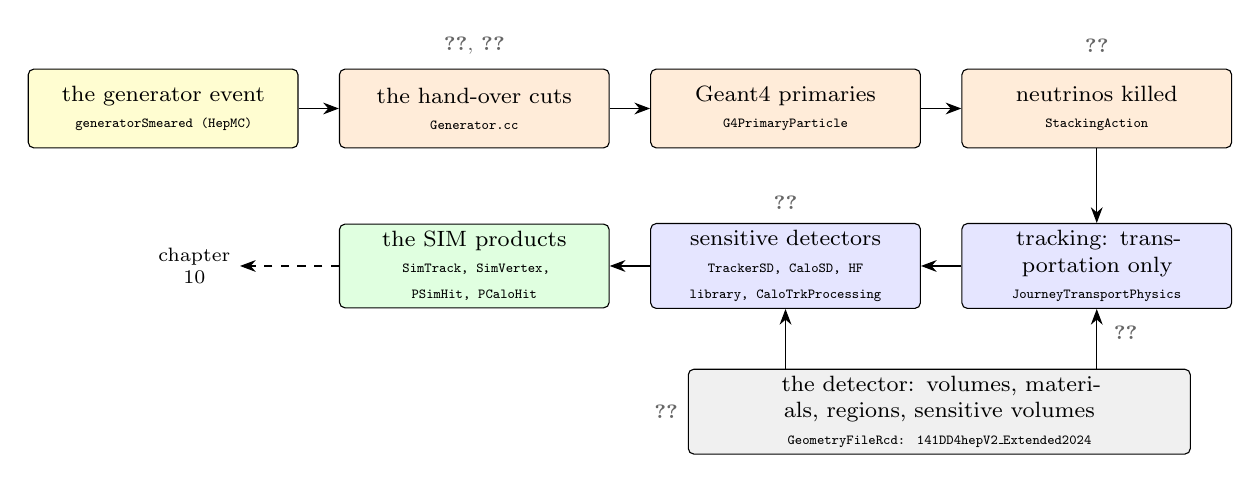
\begin{tikzpicture}[x=0.93cm, font=\footnotesize, >={Stealth[length=2mm]},
  box/.style={draw, rounded corners=2pt, minimum height=10mm, text width=3.25cm, align=center, inner sep=2.5pt},
  gen/.style={box, fill=yellow!18}, hand/.style={box, fill=orange!15}, g4/.style={box, fill=blue!10},
  prod/.style={box, fill=green!12}, geo/.style={box, fill=black!6, text width=6.2cm}]
\node[gen] (hep) at (0,1.5) {the generator event\\{\tiny\ttfamily generatorSmeared (HepMC)}};
\node[hand] (cut) at (4.25,1.5) {the hand-over cuts\\{\tiny\ttfamily Generator.cc}};
\node[hand] (pri) at (8.5,1.5) {Geant4 primaries\\{\tiny\ttfamily G4PrimaryParticle}};
\node[hand] (stk) at (12.75,1.5) {neutrinos killed\\{\tiny\ttfamily StackingAction}};
\node[g4] (trk) at (12.75,-0.5) {tracking: transportation only\\{\tiny\ttfamily JourneyTransportPhysics}};
\node[g4] (sd) at (8.5,-0.5) {sensitive detectors\\{\tiny\ttfamily TrackerSD, CaloSD, HF library, CaloTrkProcessing}};
\node[prod] (out) at (4.25,-0.5) {the SIM products\\{\tiny\ttfamily SimTrack, SimVertex, PSimHit, PCaloHit}};
\node[geo] (det) at (10.6,-2.35) {the detector: volumes, materials, regions, sensitive volumes\\{\tiny\ttfamily GeometryFileRcd: 141DD4hepV2\_Extended2024}};
\draw[->] (hep) -- (cut); \draw[->] (cut) -- (pri); \draw[->] (pri) -- (stk); \draw[->] (stk) -- (trk);
\draw[->] (trk) -- (sd); \draw[->] (sd) -- (out);
\draw[->] (det.north-|trk) -- (trk.south); \draw[->] (det.north-|sd) -- (sd.south);
\draw[->, dashed] (out.west) -- ++(-1.35,0) node[left, align=center, font=\scriptsize] {chapter\\10};
\node[font=\scriptsize, text=black!60] at (4.25,2.3) {\ref*{sec:09_cuts}, \ref*{sec:09_decays}};
\node[font=\scriptsize, text=black!60] at (12.75,2.3) {\ref*{sec:09_cuts}};
\node[font=\scriptsize, text=black!60, anchor=west] at (12.85,-1.35) {\ref*{sec:09_boundary}};
\node[font=\scriptsize, text=black!60] at (8.5,0.3) {\ref*{sec:09_hits}};
\node[font=\scriptsize, text=black!60, anchor=east] at (det.west) {\ref*{sec:09_detector}};
\end{tikzpicture}
\caption{The \code{SIM} step of this chapter: from the generator record to the simulation products. Orange: the
hand-over, which decides what Geant4 simulates; blue: the tracking and the recording, here with the physics reduced
to the transportation; grey: the detector, read from the global tag. The grey numbers are the subsections of
section~\ref{sec:09_numbers} that explain each box.}
\label{fig:09_chain}
\end{figure}

\begin{table}[!htb]
\centering\small\setlength{\tabcolsep}{4pt}
\caption{The chapter at a glance: one subsection of section~\ref{sec:09_numbers} per ingredient of figure~\ref{fig:09_chain}, what it does and what
it gives for our event.}
\label{tab:09_glance}
\begin{tabular}{@{}c>{\raggedright\arraybackslash}p{3.3cm}>{\raggedright\arraybackslash}p{6.4cm}>{\raggedright\arraybackslash}p{5.0cm}@{}}
\toprule
section & what & what it does & in our event \\
\midrule
\ref{sec:09_detector} & the detector & the 2024 geometry of the global tag: volumes, materials, sensitive volumes, regions with production cuts & 15 kinds of sensitive detector, 32 hit collections \\
\ref{sec:09_cuts} & the hand-over cuts & keeps a stable particle with $p>40\MeV$ whose straight line leaves a $2.9\cm$ cylinder before $|z|=354.8\cm$; kills the neutrinos & 634 stable particles, 571 primaries, 63 dropped \\
\ref{sec:09_decays} & the decays Pythia made & keeps the generator decays inside the beam pipe; the daughters start where the parent decayed & 29 \code{SimVertex}s, the farthest $25.8\cm$ from the collision \\
\ref{sec:09_boundary} & straight lines & every primary flies straight to the boundary between the tracker and the calorimeters & 557 of the 571 reach it \\
\ref{sec:09_hits} & hits without physics & the sensitive detectors mark each crossing; the HF shower library answers by itself & 6734 tracker hits, 1511 HF photoelectrons \\
\ref{sec:09_pileup} & the pileup & the same for the 68 in-time collisions of our bunch crossing & $12\,993$ stable, $10\,388$ primaries \\
\bottomrule
\end{tabular}
\end{table}

\begin{plainwords}[The hand-over]
Geant4 does not read \code{genParticles}; it reads the HepMC event and builds a \code{G4PrimaryParticle} for
every generator particle that passes the cuts of the \code{Generator} parameter set: a momentum above
$40\MeV$, a direction within $\abseta<5.5$, and, for particles the generator has already decayed, a decay vertex
outside a cylinder of radius $2.9\cm$ around the beam (the beam pipe), in which case Geant4 is given the
undecayed parent instead. Neutrinos pass these cuts and are killed by the \code{StackingAction}
(\code{TrackNeutrino = False}) before their first step. Each accepted particle becomes a \code{SimTrack} whose
\code{genpartIndex()} is the HepMC barcode of the generator particle, so the link between the generator record
and the simulation is kept, particle by particle. The dropped ones leave no trace in the simulation at all.
\end{plainwords}

Section~\ref{sec:09_numbers} follows figure~\ref{fig:09_chain} in six subsections, one per ingredient; each
says what the ingredient does, where its parameters are set, and what it gives for our event.

\section{From the previous chapter}

Two inputs enter (Rule E): the signal, \path{test/07_GenJet/out/step2_GENJET_07_GenJet.root}, the full
generator event of chapter~\ref{ch:06_Decay} with its generator jets, 634 stable particles carrying
$13\,600\GeV$ and $528.9\GeV$ of scalar \pt{}; and the pileup library,
\path{test/08_PU/out/step1_GEN_MinBias_08_PU.root}, the 250 minimum-bias collisions of chapter~\ref{ch:08_PU},
of which library events 72 to 139 are the 68 in-time collisions of our bunch crossing (the ones the
\code{MixingModule} of chapter~\ref{ch:10_SIM} draws into bunch crossing 0 for this signal event: seed 12345,
Poisson with mean 60, library events 1--71 going to bunch crossing $-1$), $12\,993$ stable particles with
$924.8\TeV$ and $5315\GeV$ of \pt{}.\footnote{All numbers of this chapter are in
\path{test/09_G4/out/ledger_09_G4.txt} (the output of \code{common/g4Ledger.py}),
\path{extras_09_G4.txt} (the output of \path{test/09_G4/g4Extras_09_G4.py}), \path{simAnalyzer_signal_09_G4.log}
and \path{simAnalyzer_pileup_09_G4.log}; the few extra ones (the dropped particles by kind, the displaced vertices)
were read from the SIM files with FWLite, and the dimensions of the detector from the XML of the release; the
companion lists them all in section~4.} Nothing in the generator record changes: the \code{SIM} process copies
\code{genParticles}, \code{generatorSmeared} and the jets unchanged and adds its own products under the
process name \code{SIM}: \code{SimTrack}s and \code{SimVertex}s, the \code{PSimHit} collections of the tracker
and muon system (one per subdetector and time-of-flight window, e.g.\ \code{TrackerHitsTIBLowTof}) and the
\code{PCaloHit} collections of the calorimeters (\code{EcalHitsEB}, \code{EcalHitsEE}, \code{EcalHitsES},
\code{HcalHits}). The smeared primary vertex of the signal, drawn in chapter~\ref{ch:06_Decay}, is where all
primaries start: $(0.028, -0.017, 3.11)\cm$ for the signal, $(0.029, -0.017, -0.48)\cm$ for library event~72. The
$3.11\cm$ of the signal will matter for the $\eta$ cut (section~\ref{sec:09_cuts}).

The \code{SIM} job runs with the 2025 settings of the release (global tag \code{auto:phase1\_2025\_realistic},
era \code{Run3\_2025}; the signal was generated with those of 2024, which at generator level are the same,
chapter~\ref{ch:08_PU}). The detector given to Geant4 comes from the global tag, and in this release the 2025 tag
has the geometry and the field map of 2024: \code{GeometryFileRcd} \code{Extended} is
\code{141DD4hepV2\_Extended2024} in both, the field \code{MFGeometry\_160812} at 3.8\,T too. None of the five
modifiers that \code{Run3\_2025} adds to \code{Run3\_2024} appears in \code{g4SimHits\_cfi.py}. Rerun with the
2025 settings, both files of this chapter are the 2024 ones, primary for primary and hit for hit (companion,
section~4): the 2025 detector of CMSSW\_15\_0\_5 differs from that of 2024 only in conditions and modifiers
that the simulation does not read.

The two objects to follow are the $b$ and $\bar b$ systems of chapter~\ref{ch:07_GenJet}: the nine stable
decay products of the $B^-$ ($\pt=94.3\GeV$, $\eta=-1.57$, among them the $95.5\GeV$ antineutrino) and the
16 of the $B^{*+}$ ($\pt=114.2\GeV$, $\eta=-3.75$, no neutrino).

\section{The numbers of the event}
\label{sec:09_numbers}

\subsection{The detector that Geant4 is given}
\label{sec:09_detector}

\textbf{What it does.} Geant4 cannot move a particle without a world to move it in. The world of the \code{SIM}
step is read from the global tag: the record \code{GeometryFileRcd}, label \code{Extended}, holds
\code{141DD4hepV2\_Extended2024}, the description of the 2024 detector in the DD4hep format, the same description
that the release carries as XML in \path{Geometry/CMSCommonData/data/dd4hep/cmsExtendedGeometry2024.xml} (a list of
374 included files, a few per subdetector). Each \emph{volume} has a shape, a material and a place inside a
\emph{mother} volume, so the detector is a tree. Its trunk is a chain of air-filled envelopes (\code{World}, \code{OCMS},
\code{CMSE}); inside them five mothers matter for this book (figure~\ref{fig:09_rz}): \code{BEAM}, the beam pipe;
\code{Tracker}, the silicon detectors and their supports, a cylinder of radius $123.3\cm$ and half-length
$293.2\cm$, with a thin ``nose'' around the beam pipe that continues to $|z|=355.1\cm$; \code{CALO}, the
electromagnetic and hadronic calorimeters of the barrel and the endcaps, out to $r=295\cm$; \code{MUON}, the
solenoid, the iron yoke and the muon chambers beyond; and, $11.15$\,m from the collision point on either side,
\code{VCAL}, the forward calorimeter HF, a tube from $r=12.5$ to $159.5\cm$.

Beyond shape and material, the XML attaches labels to volumes (blocks called \code{SpecPar}), and these turn a
geometry into a detector simulation. \emph{Sensitive detectors}: a volume labelled with the sensitive detector
\code{TkAccumulatingSensitiveDetector} and the read-out name \code{TrackerHitsPixelBarrel} records every step
taken inside it into that collection (the files \code{trackersens.xml}, \code{ecalsens.xml},
\code{hf.xml}, \code{muonSens.xml}). \emph{Regions}: groups of volumes with their own production cuts (the box
below). And the \emph{boundary}: the calorimeter mothers carry \code{CaloTrkProcessing}
(\path{Geometry/HcalSimData/data/CaloUtil/2021/v1/CaloUtil.xml}), which notices when a track steps into
\code{CALO}, \code{VCAL} or another calorimeter volume from one of the volumes listed as ``inside'' (\code{BEAM},
\code{Tracker}, \code{MUON}, \ldots) and stores where (section~\ref{sec:09_boundary}).

\begin{figure}[!htb]
\centering
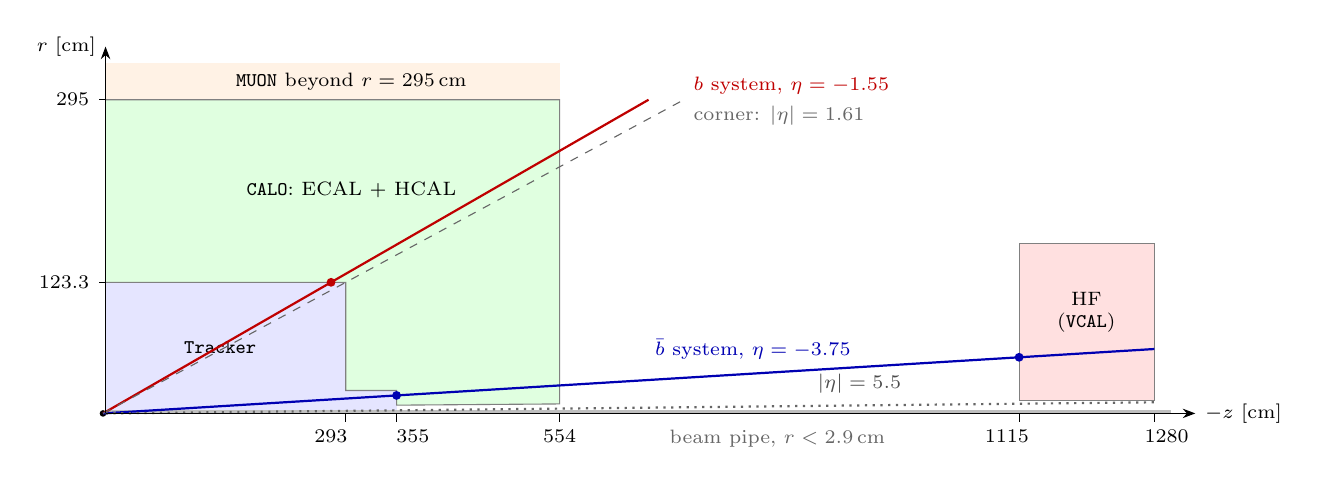
\begin{tikzpicture}[x=0.0104cm, y=0.0135cm, font=\scriptsize, >={Stealth[length=1.6mm]}]
\fill[green!12] (0,123.3) -- (293.2,123.3) -- (293.2,21.5) -- (355.15,21.5) -- (355.15,7.76) -- (554.1,8.93)
  -- (554.1,295) -- (0,295) -- cycle;
\fill[blue!10] (0,0) rectangle (293.2,123.3); \fill[blue!10] (293.2,2.9) rectangle (355.15,21.5);
\fill[red!12] (1114.95,12.495) rectangle (1280.05,159.5);
\fill[orange!10] (0,295) rectangle (554.1,330);
\fill[black!25] (0,0) rectangle (1300,2.9);
\draw[black!50] (0,123.3) -- (293.2,123.3) -- (293.2,21.5) -- (355.15,21.5) -- (355.15,7.76) -- (554.1,8.93)
  -- (554.1,295) -- (0,295);
\draw[black!50] (1114.95,12.495) rectangle (1280.05,159.5);
\node at (140,62) {\code{Tracker}};
\node at (300,210) {\code{CALO}: ECAL + HCAL};
\node at (300,312) {\code{MUON} beyond $r=295\cm$};
\node[align=center] at (1197,95) {HF\\(\code{VCAL})};
\node[anchor=north, text=black!60] at (820,-6) {beam pipe, $r<2.9\cm$};
% the lines from the signal vertex (z = +3.11 cm, drawn at x = -3.11)
\fill (-3.11,0) circle (1.2pt);
\draw[red!75!black, thick] (-3.11,0) -- (662.7,295);
\node[red!75!black, anchor=west] at (705.8,308) {$b$ system, $\eta=-1.55$};
\draw[blue!70!black, thick] (-3.11,0) -- (1280.05,60.57);
\node[blue!70!black, anchor=south] at (790,42) {$\bar b$ system, $\eta=-3.75$};
\draw[black!60, dashed] (-3.11,0) -- (705.8,295);
\node[black!60, anchor=west] at (705.8,280) {corner: $|\eta|=1.61$};
\draw[black!60, dotted, thick] (0,0) -- (1280.05,10.46);
\node[text=black!70, anchor=south] at (920,10) {$|\eta|=5.5$};
\fill[red!75!black] (275.2,123.3) circle (1.6pt); \fill[blue!70!black] (355.15,16.9) circle (1.6pt);
\fill[blue!70!black] (1114.95,52.8) circle (1.6pt);
% axes
\draw[->] (0,0) -- (1330,0) node[right] {$-z$ [cm]};
\draw[->] (0,0) -- (0,345) node[left] {$r$ [cm]};
\foreach \z in {293.2, 355.15, 554.1, 1114.95, 1280.05} \draw (\z,0) -- (\z,-8);
\node[below] at (275,-6) {293}; \node[below] at (375,-6) {355}; \node[below] at (554.1,-6) {554};
\node[below] at (1100,-6) {1115}; \node[below] at (1295,-6) {1280};
\foreach \r in {123.3, 295} \draw (0,\r) -- (-8,\r) node[left] {\r};
\end{tikzpicture}
\caption{The detector of the \code{SIM} step in the $r$--$z$ plane, for $z<0$, where both jets of the event go
(\code{cms.xml} and \code{hcalforwardalgo.xml} of the release;
the $r$ and $z$ scales differ, the muon system beyond $|z|=554\cm$ is not drawn). Blue: the \code{Tracker} volume
with its nose along the beam pipe; green: \code{CALO}; red: the HF. Lines: the straight flights from the signal
vertex at $z=+3.11\cm$ of the $b$ system (red), of the $\bar b$ system (blue), to the corner of the tracker volume
(dashed), and the line $|\eta|=5.5$ from the centre (dotted); the dots are where the systems cross into a
calorimeter volume (section~\ref{sec:09_boundary}).}
\label{fig:09_rz}
\end{figure}

\begin{plainwords}[A production cut is a range, not an energy]
Geant4 does not create every secondary particle a process could make: a photon, electron or positron that would
travel less than the \emph{production cut} of its region before stopping is not created, and its energy is
deposited on the spot. The cut is given as a distance and converted, material by material, into an energy, so
the same $1\mm$ is a larger energy in the dense crystals of the ECAL than in air. Small cuts where the detail
matters (the silicon, which must see the delta electrons that widen a cluster), large ones where it does not
(the iron of the muon system, where only the muons count): the cuts trade precision for time.
\end{plainwords}

\textbf{The parameters.} Which of the labelled sensitive detectors are switched on is decided in python, by
\code{OnlySDs} of \code{g4SimHits\_cfi.py}: for Run~3 (modifier \code{run3\_common}) 15 kinds, writing 25
\code{PSimHit} collections (the six tracker subdetectors, each in a \code{LowTof} and a \code{HighTof} collection,
the five muon technologies, the luminosity and forward detectors) and 7 \code{PCaloHit} collections (ECAL barrel,
endcap and preshower, HCAL, ZDC and two more). The regions and their production cuts are in the XML
(table~\ref{tab:09_prodcuts}); outside any region the cut is \code{DefaultCutValue = 1.0}\,cm
(\code{g4SimHits\_cfi.py}). The dimensions of figure~\ref{fig:09_rz} are constants of
\path{Geometry/CMSCommonData/data/cms/2021/v3/cms.xml}:
\code{TrackCalorR = 1.233\,m}, \code{TrackBeamZ2 = 2.932\,m}, \code{PIXNoseLength = 619.5\,mm},
\code{CalorMuonR = 2.950\,m}, and of \path{Geometry/HcalCommonData/data/hcalforwardalgo.xml}: the HF from $|z|=11.1495$ to $12.8005$\,m.

\begin{table}[!htb]
\centering\small
\caption{The regions of the 2024 geometry and their production cuts for photons, electrons and positrons
(\code{CMSCutsRegion} and \code{ProdCutsFor*} in the \code{*ProdCuts.xml} files included by
\code{cmsExtendedGeometry2024.xml}).}
\label{tab:09_prodcuts}
\setlength{\tabcolsep}{8pt}\begin{tabular}{@{}lll@{}}
\toprule
region & volumes & cut \\
\midrule
\code{BeamPipe} & the beryllium tube at the centre & $0.01\mm$ \\
\code{TrackerSensRegion} & the active silicon of the strip modules & $0.1\mm$ \\
\code{Tracker(Pixel)DeadRegion} & supports, cables, cooling & $1\mm$ \\
\code{EcalRegion} & the crystals and their housing & $1\mm$ \\
\code{APDRegion} & the photodiodes of the barrel ECAL & $0.005\mm$ \\
\code{PreshowerSensRegion} & the silicon of the preshower & $0.1\mm$ \\
\code{HcalRegion} & \code{CALO}, \code{VCAL} & $1\mm$ \\
\code{Muon} & \code{MUON} & $100\mm$ ($\gamma$), $10\mm$ ($e^\pm$) \\
\bottomrule
\end{tabular}
\end{table}

\textbf{The numbers of the event.} In this chapter the regions do nothing: with no process registered no
secondary can be created, whatever its range, and page~8 of the analyzer is empty
(figure~\ref{fig:09_boundary}, right). Of the 32 hit collections the job writes, 7 are filled for the signal: the
six \code{LowTof} tracker collections, by crossings without energy loss, and \code{HcalHits}, by the HF shower
library (section~\ref{sec:09_hits}). The geometry acts through its boundaries alone, and these decide where each
primary is recorded (section~\ref{sec:09_boundary}).

\subsection{The hand-over cuts}
\label{sec:09_cuts}

\textbf{What it does.} The class \code{Generator} (\path{SimG4Core/Generators/src/Generator.cc}) loops over the
vertices of the HepMC event and, for every particle, decides whether Geant4 gets it. A stable particle (status 1)
is tested in a fixed order: if it is a neutron, antineutron or photon so forward that it would stay in the beam
pipe for 52.8\,m, it is kept (the ``very-forward'' rule); otherwise it must have a momentum between $40\MeV$ and
$99\,999\GeV$, and its straight line must leave the beam-pipe cylinder in time (the $\eta$ cut, box below). A
particle that passes becomes a \code{G4PrimaryParticle} attached to a \code{G4PrimaryVertex} at its production
point, with \code{setGenId} set to its HepMC barcode. Particles that the generator already decayed (status 2) are
treated in section~\ref{sec:09_decays}. The \code{StackingAction}, which sees every track before Geant4 starts it,
then kills the neutrinos.

\textbf{The parameters.} Table~\ref{tab:09_cuts} lists the four reasons for which a stable particle gets no
\code{SimTrack}, with the parameter that implements it and its effect on the signal and on the 68 pileup
collisions.

\begin{table}[htb]
\centering\small\setlength{\tabcolsep}{4pt}
\caption{Why a stable particle gets no \code{SimTrack}: the cuts of \code{g4SimHits\_cfi.py} and what they remove
from the signal and from the 68 in-time pileup collisions (\code{ledger\_09\_G4.txt}; the split by kind from the
FWLite extras of the companion). The last line is the exception that keeps very forward neutrals.}
\label{tab:09_cuts}
\begin{tabular}{p{1.9cm}p{3.5cm}p{4.0cm}p{4.7cm}}
\toprule
cut & parameter & signal (634 stable) & 68 collisions ($12\,993$ stable) \\
\midrule
$\abseta>5.5$ & \code{Generator}: \code{ApplyEtaCuts}, \code{MinEtaCut} / \code{MaxEtaCut} $=\mp5.5$; the line inside $r<2.9\cm$ at $|z|=355\cm$ & 56, $6581\GeV$, $19.6\GeV$ \pt{}: 27 charged hadrons (3869, of which 4 protons 1277), 8 neutral hadrons (1580), 21 photons (1132); $5.52<\abseta<8.04$ & 2492, $706.0\TeV$, $851.4\GeV$ \pt{}: 1228 charged hadrons ($517.0\TeV$, 132 protons with $226.2\TeV$), 251 neutral hadrons (98.7), 994 photons (89.4), 19 electrons (0.9); 211 beyond $\abseta=8.2$ ($364.9\TeV$) \\
$p<40\MeV$ & \code{ApplyPCuts}, \code{MinPCut = 0.04} & 6 photons from $\pi^0$, $0.2\GeV$ & 98 (94 photons, 2 charged hadrons, 2 electrons), $2.7\GeV$ \\
neutrino & \code{StackingAction}: \code{TrackNeutrino = False} & 1 ($\bar\nu_e$ of the $B^-$: $95.5\GeV$, $\pt=37.5$) & 7, $57.5\GeV$ \\
other & the $\eta$ line from a displaced vertex & 0 & 8 ($166.4\GeV$): 4 photons, 4 charged hadrons at $\abseta=5.48$--$5.50$ \\
\midrule
kept beyond 5.5 & forward $n$, $\bar n$, $\gamma$ inside $r<2.9\cm$ at $|z|=52.8$\,m & 2: a neutron ($151\GeV$, $\eta=9.72$), a $\pi^+$ ($84.6\GeV$, $\eta=-5.50$) & 168, $134.2\TeV$ \\
\bottomrule
\end{tabular}
\end{table}

\begin{plainwords}[The $\eta$ cut is a line, not an angle]
The cut does not test $\abseta<5.5$. It follows the straight line of the particle from its production vertex to
$|z| = 2.9\cm\times\sinh5.5 = 2.9\times122.3 = 354.8\cm$ and drops the particle if the line is then still inside
the $2.9\cm$ cylinder (\code{RDecLenCut}). From the nominal collision point this is the same as $\abseta>5.5$,
since a line of pseudorapidity $\eta$ is at $r=|z|/\sinh|\eta|$. Our vertex is at $z=+3.11\cm$. The $\pi^+$ of
$84.6\GeV$ at $\eta=-5.5002$ flies towards negative $z$: from the nominal point it would arrive at
$r=354.8/\sinh5.5002=2.899\cm$, $10\um$ inside, and be dropped; from our vertex it flies $357.9\cm$ and arrives at
$2.940\cm$: kept. The photon of $12.9\GeV$ at $\eta=-5.5240$ arrives at $2.887\cm$: dropped. Towards positive $z$
the vertex shortens the flight: the $K^0_S$ at $\eta=+5.4824$ arrives at $2.903\cm$ instead of $2.951\cm$, kept by
$30\um$. The very-forward rule uses the same construction with $\eta=8.2$: $2.9\cm\times\sinh8.2 = 2.9\times1820 =
5279\cm$, the 52.8\,m of the table.
\end{plainwords}

\textbf{The numbers of the event.} The $\eta$ cut is where almost all the energy goes: 56 particles with
$6581\GeV$ of the signal, at $5.52<\abseta<8.04$, and in the pileup eight particles at $\abseta = 5.48$--$5.50$
with vertices displaced by $1$--$6\cm$ in $z$ are dropped although their momentum points just inside $5.5$ (the
``other'' column of the ledger, the box above at work). The very-forward rule
(\code{EtaCutForHector = 8.2}) hands the $151\GeV$ neutron at $\eta = 9.72$ of the signal and 168 particles with
$134.2\TeV$ of the 68 pileup collisions to Geant4 for the Zero Degree Calorimeter; they are later stopped in the
dead regions of the beam line (\code{DeadRegions = QuadRegion, InterimRegion}). The $40\MeV$ cut removes six
photons from $\pi^0$ decays ($27$--$38\MeV$), $0.2\GeV$ in all. The one neutrino is the $\bar\nu_e$ of the
semileptonic $B^-$ decay with $95.5\GeV$ and $37.5\GeV$ of \pt{}: the $b$ system enters Geant4 with 8 of its 9
particles and $56.8$ of its $94.3\GeV$ of \pt{}, while the $\bar b$ system enters complete, 16 of 16,
$114.2\GeV$. The net $b+\bar b$ \pt{}, $20.3\GeV$ at hadron level, is $57.5\GeV$ among the primaries: a detector
cannot see the neutrino, and the imbalance it will measure for this event is decided here.

\subsection{The decays that Pythia already made}
\label{sec:09_decays}

\textbf{What it does.} Pythia8 decays every unstable hadron whose mean decay length $c\tau$ is below $10\mm$ and
leaves the others to the detector simulation; the $B$ and $D$ mesons of our event ($c\tau$ of $0.5$ and
$0.12\mm$) are decayed by the generator, the $K^0_S$ ($27\mm$), the $\Lambda$ ($79\mm$), the charged pions and
kaons (metres) are not. A decayed hadron stays in the record with status 2 and a decay vertex. The
\code{Generator} then asks where that vertex is. Inside the $2.9\cm$ cylinder around the beam, the decay
happened in the vacuum of the beam pipe and is kept as Pythia made it: Geant4 gets the daughters as primaries,
starting at the decay point, which is stored as a \code{SimVertex} without a parent track. Outside the cylinder the
parent itself is given to Geant4, with Pythia's decay attached as a ``predefined decay channel'', so that it decays
where the generator decided but inside the material, after having crossed it.

\textbf{The parameters.} \code{ParticleDecays:limitTau0 = on}, \code{ParticleDecays:tau0Max = 10} (in mm,
\path{Configuration/Generator/python/Pythia8CommonSettings_cfi.py}); \code{RDecLenCut = 2.9} (cm) in the
\code{Generator} parameter set; its partner \code{LDecLenCut = 30.0}, a length in $z$, is read and never used
(section~5).

\textbf{The numbers of the event.} The file holds 29 \code{SimVertex}s for the signal although nothing decayed in
Geant4: the smeared primary vertex and 28 generator decay vertices, all inside the cylinder, so every daughter of
the event starts as a primary. Table~\ref{tab:09_decays} follows the three weak decays of the two $b$ systems. The
distance a particle flies before it decays is a random number, exponential with mean $\beta\gamma c\tau$, and the
three in the table illustrate it: the $B^+$ flew half of its mean, the $\bar D^0$ more than twice its own, which
happens one time in ten. The $\bar D^0$ of the $\bar b$ jet decayed $25.8\cm$ from the collision, still inside the
beam pipe at $r = 1.2\cm$, because a particle at $\eta=-3.76$ moves $21$ times faster along the beam than away from
it. The primaries of these decays start from those points (figure~\ref{fig:09_rz}).

\begin{table}[!htb]
\centering\small\setlength{\tabcolsep}{4pt}
\caption{The three weak decays of the $b$ and $\bar b$ systems, kept from the generator (FWLite extras of the
companion; $m$ and $c\tau$ from the Particle Data Group: $B^\pm$ $5.279\GeV$, $491\um$; $D^0$ $1.865\GeV$,
$123\um$). The flight is measured from the point where the hadron was made.}
\label{tab:09_decays}
\begin{tabular}{@{}l rrr r r rr l@{}}
\toprule
hadron & $E$ & \pt{} & $\eta$ & $\beta\gamma$ & mean $\beta\gamma c\tau$ & flight & decay $(r,z)$ & daughters \\
 & [GeV] & [GeV] & & & [cm] & [cm] & [cm] & \\
\midrule
$B^-$ ($b$ jet) & 235.9 & 94.3 & $-1.57$ & 44.7 & 2.2 & 0.78 & $(0.32, 2.39)$ & $\bar\nu_e$, $e^-$, $D_0^*(2300)^0$ \\
$B^+$ ($\bar b$ jet) & 2388.2 & 112.6 & $-3.75$ & 452 & 22.2 & 11.7 & $(0.55, -8.60)$ & $\bar D^{*0}$, $\pi^+$, $\pi^0$, $K^0$, $\bar K^{*0}$ \\
$\bar D^0$ (from the $B^+$) & 911.9 & 42.4 & $-3.76$ & 489 & 6.0 & 14.1 & $(1.21, -22.66)$ & $\bar K^0$, $\pi^-$, $\pi^+$, $\pi^0$, $\pi^0$ \\
\bottomrule
\end{tabular}
\end{table}

\subsection{Straight lines to the calorimeters}
\label{sec:09_boundary}

\textbf{What it does.} With no process registered, the only thing Geant4 does to a particle is the
\emph{transportation}: it moves it in a straight line to the next boundary between two volumes, then to the next,
until the particle leaves the world or reaches the time limit of the \code{SteppingAction}
(\code{MaxTrackTime = 500}\,ns). The step that takes a track from an ``inside'' volume into a calorimeter
volume is seen by \code{CaloTrkProcessing}, which writes the point and the momentum into the \code{SimTrack} (\code{trackerSurfacePosition()}, \code{trackerSurfaceMomentum()}, \code{crossedBoundary()}).
This is the moment at which the truth of a particle passes from the tracker to the calorimeters: in the next
chapters a shower in the ECAL is credited to the track that crossed here, not to the electrons it is made of.

\textbf{The parameters.} The surfaces are those of figure~\ref{fig:09_rz}. Two numbers follow from them by
geometry. Seen from our vertex at $z=+3.11\cm$, the corner of the tracker volume, $(r,z)=(123.3,-293.2)\cm$, is at
$\eta=-\sinh^{-1}(296.3/123.3) = -1.61$: on the negative side a particle leaves the tracker through the barrel
cylinder if $\abseta<1.61$, through the endcap disk if it is beyond. And the hole of the HF closes the acceptance:
a line from the centre reaches the inner radius of the HF, $12.5\cm$, at its back face, $|z|=1280\cm$, if
$\sinh\abseta = 1280/12.5 = 102.4$, that is $\abseta = 5.32$. A particle beyond that passes through the hole of
every calorimeter.

\textbf{The numbers of the event.} 557 of the 571 primaries cross into a calorimeter volume, with exactly their
production momentum: no field, no material effect. Table~\ref{tab:09_boundary} says through which surface. The $b$
system, at $\eta=-1.55$, is $0.06$ from the corner: 7 of its 8 primaries leave the tracker through the barrel
cylinder between $z=-240$ and $-292\cm$, and one photon of $1.5\GeV$ at $\eta=-1.68$ through the endcap disk at
$r=114\cm$. The $b$ jet that the calorimeters and the trigger of chapters~\ref{ch:11_DIGI} and~\ref{ch:12_L1T} find on
the barrel--endcap boundary sits there already in the geometry of the tracker. The $\bar b$ system crosses, all 16, through the ring at the end of the nose,
$z=-355.1\cm$, at $r=15.4$--$20.3\cm$, and flies another $7.6$\,m to the front face of the HF. The 14 primaries
that never cross are 13 particles at $5.34<\abseta<5.50$, accepted by the $\eta$ cut but beyond the $5.32$ of the
HF hole, and the forward neutron. The usable acceptance of the simulation therefore ends at $\abseta\approx5.3$,
not at the $5.5$ of the cut; the 16 signal particles with $5.2<\abseta<5.5$ ($836\GeV$) are all accepted and only
three of them reach a calorimeter volume.

\begin{table}[!htb]
\centering\small
\caption{Where the primaries cross into a calorimeter volume (\code{extras\_09\_G4.txt}, from
\code{SimTrack::trackerSurfacePosition}), for the signal and for library event 72; the $\abseta$ range is that of
the signal primaries through the surface.}
\label{tab:09_boundary}
\begin{tabular}{@{}lll rr@{}}
\toprule
surface & where & $\abseta$ (signal) & signal & event 72 \\
\midrule
barrel cylinder & $r=123.3\cm$, $|z|<293.2\cm$ & 0.01--1.61 & 172 & 54 \\
endcap disk & $|z|=293.2\cm$, $r=23$--$122\cm$ & 1.60--3.23 & 228 & 66 \\
end of the nose & $|z|=355.1\cm$, $r=7.8$--$21.3\cm$ & 3.50--4.51 & 98 & 18 \\
front face of the HF & $|z|=1114.9\cm$, $r=13$--$85\cm$ & 3.26--5.16 & 36 & 9 \\
inner walls along the beam pipe & $r=7.8$--$12.5\cm$, $|z|=356$--$1277\cm$ & 4.51--5.32 & 23 & 8 \\
\midrule
no crossing & & 5.34--5.50, 9.72 & 14 & 9 \\
all primaries & & & 571 & 164 \\
\bottomrule
\end{tabular}
\end{table}

\begin{figure}[!htb]
\centering
\begin{subfigure}[t]{0.495\textwidth}
\includegraphics[width=\textwidth]{09_G4/out/simAnalyzer_signal_09_G4_page-07.png}
\caption{the 557 primaries at the boundary, marker at the crossing point: page~6 again.}
\end{subfigure}\hfill
\begin{subfigure}[t]{0.495\textwidth}
\includegraphics[width=\textwidth]{09_G4/out/simAnalyzer_signal_09_G4_page-08.png}
\caption{the secondaries created by Geant4: none, only the primaries as grey dots.}
\end{subfigure}
\caption{The signal through the transport-only Geant4, pages 7 and 8 of \code{simAnalyzer\_signal\_09\_G4.pdf}
(\code{\_page-07.png}, \code{\_page-08.png}). Without field and physics every primary arrives where it was
aimed and creates nothing: the two pages that will change most in chapter~\ref{ch:10_SIM}.}
\label{fig:09_boundary}
\end{figure}

\subsection{Hits without physics}
\label{sec:09_hits}

\textbf{What it does.} A sensitive detector is the code that a sensitive volume calls at every step taken inside
it. The tracker one (\code{TkAccumulatingSensitiveDetector}) makes one \code{PSimHit} per crossing of a silicon
sensor: entry and exit point in the frame of the sensor, energy loss, time of flight, the track that made it.
Normally a crossing with no energy loss is not recorded; here \code{TrackerSD.ZeroEnergyLoss = True} records it
anyway, so that the transport-only run shows which sensors each straight line crosses. The hits are split by their
time of flight into a \code{LowTof} and a \code{HighTof} collection, the in-time and the late ones, at three times
the shaping time of the strip electronics. The calorimeter one (\code{CaloSD} and its daughters \code{ECalSD},
\code{HCalSD}) adds the energy deposited in a cell by a track into one \code{PCaloHit} per cell, track and time
slice; with no physics nothing is deposited, except in the HF (box below).

\begin{plainwords}[The HF shower library]
The HF is steel with quartz fibres in it, and it sees the Cherenkov light that the charged particles of a shower
make in the fibres: far too many photons to follow one by one in every event. CMS simulated such showers once,
electromagnetic and hadronic ones at a set of energies, and stored the light captured in the fibres (the file
\code{HFShowerLibrary\_run3\_v7.root}). When a photon, electron or hadron (not a muon) takes its first step in
the HF, \code{HCalSD} (\code{getFromHFLibrary}) takes one stored shower from each of the two library energies
around the particle's energy, keeps their photons in proportion, turns them to the particle's direction and
position, applies the attenuation along the fibre, books each surviving photon as a photoelectron, a hit of
``$1\GeV$'' in its cell, and kills the particle. The library is called by the sensitive detector, not by a
physics process, which is why the HF answers even here.
\end{plainwords}

\textbf{The parameters.} \code{TrackerSD}: \code{ZeroEnergyLoss = False} by default (\code{True} by the customise
line of this chapter), \code{ElectronicSigmaInNanoSeconds = 12.06}, hence the \code{LowTof}/\code{HighTof} split at
$3\times12.06 = 36.2\ns$, \code{EnergyThresholdForPersistencyInGeV = 0.2}. \code{CaloSD}: \code{EminHits = 15} and
$10\MeV$ for EB and EE, \code{TmaxHits = 500}\,ns. \code{HFShower}: \code{UseShowerLibrary = True}, the library
file set by the modifier \code{run3\_HFSL} of \path{Geometry/HcalSimData/python/HFParameters_cff.py}.

\textbf{The numbers of the event.} The tracker records 6734 \code{PSimHit}s (PXB 908, PXF 829, TIB 960, TID
679, TOB 860, TEC 2498), all in the \code{LowTof} collections (time of flight $0.2$ to $14.0\ns$), from 375
primaries, 193 charged and 182 neutral: a photon ``hits'' a sensor here because it crosses it. The count is pure
geometry. A straight track at $\abseta<1$ crosses the 4 pixel layers, the 4 layers of the inner barrel (TIB) and the 6 of the outer
barrel (TOB); the first two layers of TIB and of TOB carry two sensors back to back, one with its strips at a
small stereo angle, so the track crosses $4+6+8=18$ sensors. The 38 charged primaries with $\abseta<1$ have $18.7$
hits on average (17 to 21: neighbouring modules overlap a little so as to leave no gap), the 47 photons $18.6$.
Between $\abseta=1$ and 2, where a track crosses barrel layers and then endcap disks, the average is $21.3$ and
the most, 32, belongs to a photon at $\eta=-1.96$. The $b$ system leaves 179 hits; the $\bar b$ system, at
$\eta=-3.75$, none.

Of the calorimeters only the HF responds: 746 \code{PCaloHit}s in 459 cells, 1511 photoelectrons, from 144
primaries that carried $4266\GeV$ into it, $0.35$ photoelectrons per GeV. A shower is not an average: the
$\pi^+$ of $643\GeV$ of the $\bar b$ system gives 321 photoelectrons ($0.50$ per GeV), a $K^0_L$ of $241\GeV$ next
to it 84 ($0.35$), a $\pi^+$ of $165\GeV$ 46 ($0.28$). The $\bar b$ system puts 760 photoelectrons into 39 cells.
Figure~\ref{fig:09_hits} shows both pages.

\begin{figure}[htb]
\centering
\begin{subfigure}[t]{0.495\textwidth}
\includegraphics[width=\textwidth]{09_G4/out/simAnalyzer_signal_09_G4_page-09.png}
\caption{the 6734 tracker \code{PSimHit}s, zero energy loss, by subdetector; red: the $b$ system.}
\end{subfigure}\hfill
\begin{subfigure}[t]{0.495\textwidth}
\includegraphics[width=\textwidth]{09_G4/out/simAnalyzer_signal_09_G4_page-10.png}
\caption{the \code{PCaloHit}s: only the 459 HF cells of the shower library; blue: the $\bar b$ system.}
\end{subfigure}
\caption{The signal through the transport-only Geant4: the tracker hits (left) and the calorimeter hits (right),
pages 9 and 10 of \code{simAnalyzer\_signal\_09\_G4.pdf} (\code{\_page-09.png}, \code{\_page-10.png}). Pages 1--5
of the same PDF are the five generator stages, pages 6--8 the primaries, the boundary crossing and the (empty) list
of secondaries.}
\label{fig:09_hits}
\end{figure}


\subsection{The pileup collisions}
\label{sec:09_pileup}

\textbf{What it does.} The library of chapter~\ref{ch:08_PU} goes through the same transport-only Geant4, all 250
collisions, each from its own smeared vertex. Nothing is mixed yet: each collision is an event of its own, and
the ledger sums the 68 that the mixing of chapter~\ref{ch:10_SIM} will put into our bunch crossing.

\textbf{The parameters.} Those of the signal, with the Geant4 seed of the library, \code{PUSEED}$+2 = 20243$
(only the HF shower library draws random numbers in this run).

\textbf{The numbers of the event.} Library event~72, the first in-time collision (figure~\ref{fig:09_pileup}), has
192 stable particles of which 164 become primaries; 27 are beyond $\abseta=5.5$ with $9041$ of its $13\,600\GeV$
(three of them beyond $8.2$, among them a $\Lambda$ of $3414\GeV$ at $\eta=9.85$), one photon is below $40\MeV$,
and four forward neutrals with $3749\GeV$ are kept by the very-forward rule. 155 of the 164 reach the
calorimeter boundary (table~\ref{tab:09_boundary}: 54 through the barrel cylinder, 66 through the endcap disk);
the collision leaves 1965 tracker hits and 153 HF hits with 192 photoelectrons in 135 cells. Over the 68
collisions the number of primaries runs from 0 (library event 124, a diffractive collision with 6 stable
particles, all beyond $\abseta=5.5$) to 470 (event 94, 547 stable particles), 153 on average.

\begin{figure}[!htb]
\centering
\begin{subfigure}[t]{0.495\textwidth}
\includegraphics[width=\textwidth]{09_G4/out/simAnalyzer_pileup_09_G4_page-06.png}
\caption{the 164 primaries and the 28 stable particles without a \code{SimTrack} (grey crosses).}
\end{subfigure}\hfill
\begin{subfigure}[t]{0.495\textwidth}
\includegraphics[width=\textwidth]{09_G4/out/simAnalyzer_pileup_09_G4_page-09.png}
\caption{its 1965 tracker \code{PSimHit}s by subdetector, zero energy loss.}
\end{subfigure}
\caption{One pileup collision through the transport-only Geant4: library event~72, pages 6 and 9 of
\code{simAnalyzer\_pileup\_09\_G4.pdf} (\code{\_page-06.png}, \code{\_page-09.png}). No jet, no $b$ system: an even
spray of soft particles.}
\label{fig:09_pileup}
\end{figure}

\section{Ledger and display}

Table~\ref{tab:09_ledger} is the ledger of the hand-over, by region and by kind, for the signal, for the 68
collisions and for their sum. For the signal the stage removes 63 of 634 particles, but $6677\GeV$ of
$13\,600$: 90\,\% of the particles, 89\,\% of the \pt{} and 51\,\% of the energy go into Geant4. Everything in
$2.5<\abseta<5.5$ passes untouched; the central region loses the six soft photons and the neutrino; beyond
$5.5$ only the forward neutron and the border $\pi^+$ survive. For the pileup the picture is more extreme:
80\,\% of the particles and 84\,\% of the \pt{} enter, but only 24\,\% of the energy, because $840$ of the
$925\TeV$ of a bunch crossing's minimum-bias collisions sit beyond $\abseta=5.5$ in the beam remnants and
$706\TeV$ of them are never simulated. What remains per collision is on average 153 primaries, $3.2\TeV$
and $66\GeV$ of \pt{}, of which 70 particles and $32\GeV$ of \pt{} in the tracker region. The sum of signal and
68 collisions is what chapter~\ref{ch:10_SIM} will mix: $10\,959$ primaries with $225\TeV$ and $4957\GeV$ of
\pt{}, the signal being 5\,\% of the particles and 10\,\% of the \pt{} of its own bunch crossing.

\begin{table}[htbp]
\centering\scriptsize\setlength{\tabcolsep}{2.5pt}
\caption{The ledger of the hand-over (\code{ledger\_09\_G4.txt}; the regions and kinds from the FWLite extras of
the companion): the stable particles before and the Geant4 primaries after, $n$ / $E$ [GeV] / \pt{} [GeV],
for the signal and for the 68 in-time pileup collisions; the last block gives the fractions handed over, the dropped
particles by the reasons of table~\ref{tab:09_cuts}, and the sum.}
\label{tab:09_ledger}
\begin{tabular}{lrrrrrrcrrrrrr}
\toprule
 & \multicolumn{6}{c}{signal} & & \multicolumn{6}{c}{68 pileup collisions} \\
\cmidrule(lr){2-7}\cmidrule(lr){9-14}
 & \multicolumn{3}{c}{before: stable} & \multicolumn{3}{c}{after: primaries} & & \multicolumn{3}{c}{before: stable} & \multicolumn{3}{c}{after: primaries} \\
 & $n$ & $E$ & \pt{} & $n$ & $E$ & \pt{} & & $n$ & $E$ & \pt{} & $n$ & $E$ & \pt{} \\
\midrule
$\abseta<2.5$     & 316 & 733.8 & 278.7 & 309 & 638.1 & 241.1 & & 4864 & 5519 & 2179.4 & 4765 & 5506 & 2173.6 \\
$2.5<\abseta<3.0$ & 55 & 193.1 & 24.6 & 55 & 193.1 & 24.6 & & 1037 & 3597 & 449.2 & 1035 & 3597 & 449.2 \\
$3.0<\abseta<5.2$ & 189 & 5019.6 & 197.4 & 189 & 5019.6 & 197.4 & & 3996 & 58\,413 & 1674.3 & 3992 & 58\,367 & 1672.7 \\
$5.2<\abseta<5.5$ & 16 & 836.4 & 7.8 & 16 & 836.4 & 7.8 & & 436 & 17\,054 & 160.3 & 428 & 16\,888 & 158.9 \\
$\abseta>5.5$     & 58 & 6817.1 & 20.3 & 2 & 235.9 & 0.7 & & 2660 & 840\,217 & 851.4 & 168 & 134\,196 & 31.1 \\
\midrule
charged hadrons & 303 & 7167.7 & 259.1 & 276 & 3298.6 & 247.8 & & 5911 & 572\,735 & 3087.8 & 4677 & 55\,664 & 2596.3 \\
neutral hadrons & 56 & 3449.9 & 84.7 & 48 & 1869.8 & 81.1 & & 1088 & 179\,328 & 749.7 & 837 & 80\,592 & 627.3 \\
photons         & 273 & 2875.9 & 142.7 & 246 & 1743.7 & 137.9 & & 5900 & 171\,676 & 1458.8 & 4808 & 82\,175 & 1251.9 \\
electrons, muons & 1 & 10.9 & 5.0 & 1 & 10.9 & 5.0 & & 87 & 1004 & 12.6 & 66 & 121.4 & 10.1 \\
neutrinos       & 1 & 95.5 & 37.5 & 0 & 0 & 0 & & 7 & 57.5 & 5.6 & 0 & 0 & 0 \\
\midrule
all & 634 & 13\,600.0 & 528.9 & 571 & 6923.0 & 471.7 & & 12\,993 & 924\,800 & 5314.6 & 10\,388 & 218\,553 & 4485.6 \\
\bottomrule
\end{tabular}

\medskip
\begin{tabular}{ll}
\toprule
signal & handed over: 90.1\,\% of the particles, 50.9\,\% of $E$, 89.2\,\% of \pt{}; \\
 & dropped ($E$ in GeV): 56 beyond $\abseta=5.5$ (6581.3), 6 below $40\MeV$ (0.2), 1 neutrino (95.5) \\
68 collisions & handed over: 80.0\,\% of the particles, 23.6\,\% of $E$, 84.4\,\% of \pt{}; \\
 & dropped: 2492 beyond $\abseta=5.5$ ($706\,021$), 98 below $40\MeV$ (2.7), 7 neutrinos (57.5), 8 other (166.4) \\
signal + pileup & before: $13\,627$ stable particles, $938\,400\GeV$, $5843.5\GeV$ of \pt{}; \\
 & after: $10\,959$ primaries, $225\,476\GeV$, $4957.3\GeV$ of \pt{} (80.4\,\%, 24.0\,\%, 84.8\,\%); \\
 & dropped: 2548 beyond $\abseta=5.5$ ($712\,602$), 104 below $40\MeV$ (2.9), 8 neutrinos (153.0), 8 other (166.4) \\
\bottomrule
\end{tabular}
\end{table}

Figure~\ref{fig:09_prim} is the $\eta$--$\phi$ display of the event at this stage: the 571 primaries in the
colour of their kind, marker size growing with \pt{}, the $b$ system in red at $(\eta,\phi) = (-1.55, -2.09)$
and the $\bar b$ system in blue at $(-3.75, 1.01)$, and the 63 particles without a \code{SimTrack} as grey
crosses. The crosses are where the ledger says: a column at each border of the plot (38 of the 56 forward
particles sit beyond the $|\eta|=6$ edge of the display and are drawn on it), six faint ones scattered over the
centre (the photons below $40\MeV$) and one at the $b$ system (the neutrino). Compared with page~5 of the
same PDF, the stage-5 display of chapter~\ref{ch:06_Decay}, nothing has moved: the hand-over is a selection,
not a transformation, and page~7 (figure~\ref{fig:09_boundary}) is the same picture again.

\begin{figure}[htbp]
\centering
\includegraphics[width=0.7\textwidth]{09_G4/out/simAnalyzer_signal_09_G4_page-06.png}
\caption{The signal handed to Geant4 (\code{simAnalyzer\_signal\_09\_G4\_page-06.png}): the 571 primaries
(\code{SimTrack}s with a generator link) by kind, the $b$ and $\bar b$ systems in red and blue with their
vector sum (star), and the 63 stable particles without a \code{SimTrack} as grey crosses (56 beyond
$\abseta=5.5$, 6 below $40\MeV$, 1 neutrino). The right panel marks the SIM stage of this sample: transport
only.}
\label{fig:09_prim}
\end{figure}

\begin{plainwords}[What the pileup brings into Geant4]
A minimum-bias collision carries $13.6\TeV$, the same as the signal, but almost all of it goes down the beam
pipe: in the 68 collisions $840\TeV$ of $925$ are beyond $\abseta=5.5$, where there is no detector, and the
hand-over drops $706\TeV$ of them before Geant4 does a single step. What enters is small per collision, 153
particles and $66\GeV$ of \pt{}, but there are 68 of them: $4486\GeV$ of \pt{} against the $472$ of the
signal. In the tracker region alone the pileup primaries carry $2174\GeV$ of \pt{} to the signal's $241$. In the
tracker region the 68
collisions lay down $2174/(5\times2\pi) = 69\GeV$ of \pt{} per unit of $\eta$--$\phi$ area; at the HL-LHC, with
200 collisions, the same hand-over would deliver about $200\GeV$.
\end{plainwords}

\FloatBarrier
\section{Open problems for Phase-2}

The hand-over is configured once for all eras in \path{SimG4Core/Application/python/g4SimHits_cfi.py}. A look
through that file and the Phase-2 modifiers it imports gives the following.

\textbf{The $\eta$ cut is not era-dependent.} \code{Generator.MinEtaCut = -5.5}, \code{MaxEtaCut = 5.5} and
\code{RDecLenCut = 2.9} carry no modifier at all; the only places where the cut changes are
\path{Configuration/StandardSequences/python/SimWithCastor_cff.py} ($-7.0$ to $5.5$, for the CASTOR years) and
\path{SimG4Core/Application/python/NeutronBGforMuons_cff.py} ($\pm7.0$, a neutron-background study). The Phase-2
detector list of \code{phase2\_common} in the same file (\code{OnlySDs}) adds the HGCal, the MTD
(\code{MtdSensitiveDetector}), the HFNose and keeps the ZDC, the BCM1F and the PLT; the Phase-2 Level-1 regions of
\path{L1Trigger/Phase2L1ParticleFlow/python/l1ctLayer1_cff.py} put the HGCal at $1.5<\abseta<3.0$ and the HF at
$3.0<\abseta<5.5$. In this event the particles with $5.2<\abseta<5.5$ (16, $836\GeV$) are accepted and 13 of
them never enter a calorimeter volume (the hole of the HF, section~\ref{sec:09_boundary}); whether the
Phase-2 geometry closes that gap could not be established from the python. The very-forward rule that keeps neutrons and photons aimed at the ZDC
(\code{EtaCutForHector = 8.2}, 168 primaries with $134\TeV$ in our 68 collisions) runs at the HL-LHC as it does
now, with \code{SteppingAction.CMStoZDCtransport = False}, so these particles are simulated up to the beam-line
dead regions and then killed: CPU spent on tracks that produce nothing.

\textbf{The $40\MeV$ cut and the decay cylinder.} \code{MinPCut = 0.04} has no modifier either. It is a cut
on the total momentum, below the response of any detector of Run~3; for the HGCal (\code{HGCSD.EminHit = 0.0})
and the MTD (\code{MtdSD.EminHit = 0.0}) the sensitive detectors keep every deposit, so the $40\MeV$ remains the
only lower limit of what is simulated, and it has not been revisited. \code{LDecLenCut = 30.0} is read in
\code{Generator.cc} into a local variable, printed and never used: the decay cylinder is defined by its radius
alone, $2.9\cm$, the Run-3 beam pipe. The $\bar D^0$ of this event decayed at $r = 1.2\cm$, $z = -22.7\cm$,
inside it, so Pythia's decay was kept; a $2.9\cm$ cylinder of unlimited length also keeps generator decays that
happen metres down the beam pipe. The radius of the Phase-2 beam pipe and of the first inner-tracker layer is
not in a python file of the release and I could not establish whether $2.9\cm$ still corresponds to it.

\textbf{The StackingAction thresholds.} The Russian roulette of the \code{StackingAction} kills low-energy
photons (\code{RusRoGammaEnergyLimit = 5} MeV) and neutrons (\code{RusRoNeutronEnergyLimit = 10} MeV) with a
survival probability per region: $0.3$ for photons and $0.1$ for neutrons in the ECAL, HCAL, muon iron,
preshower and world. The two Phase-2 entries, \code{RusRoHGcalGamma = 1.3} and \code{RusRoHGcalNeutron = 1.1},
are not tuned probabilities: \path{SimG4Core/Application/src/StackingAction.cc} applies the roulette only when
the value is below 1 (line 341, \code{prob < 1.0}) and only registers the \code{HGCalRegion} in that case
(line 399), so these values switch the roulette off in the HGCal. Every photon above the production cut and
every neutron is tracked there, which is the right choice for a calorimeter with $0.5$ and $1$\,cm$^2$ cells
and timing, and the CPU cost of it at PU 200 is paid in full. The heavy-particle thresholds
(\code{NeutronThreshold}, \code{ProtonThreshold}, \code{IonThreshold} $=30\MeV$) act only with
\code{KillHeavy = True}, which is off.

\textbf{Physics list and Geant4 version.} The signal log carries the banner ``Geant4 version Name:
geant4-11-02-patch-02 [MT] (21-June-2024)'', i.e.\ the \code{geant4} tool 11.2.2 of this release. The list is
\code{SimG4Core/Physics/FTFP\_BERT\_EMM} for every era (no modifier in \code{g4SimHits\_cfi.py}; only the
CPU-benchmark and neutron-background customisations switch to \code{FTFP\_BERT}, \code{FTFP\_BERT\_XS\_EML},
\code{FTFP\_BERT\_HP\_EML}): \path{SimG4Core/PhysicsLists/plugins/FTFPCMS_BERT_EMM.cc} registers the CMS
electromagnetic constructor \code{CMSEmStandardPhysics}, \code{G4DecayPhysics}, elastic, FTFP/Bertini
(\code{EminFTFP = 3}, \code{EmaxBERT = 6}, \code{EmaxBERTpi = 12} GeV) and stopping physics. The EM options
\code{G4TransportWithMSC = 2}, \code{G4GammaGeneralProcess = True}, \code{G4HepEmActive = False} are the same
for Phase-2. Whether the HGCal needs a different EM constructor (the \code{\_EMMT} and \code{\_EMM\_TRK}
variants exist next to it) could not be established from the configuration.

\textbf{The time windows.} \code{common\_maximum\_time} sets \code{MaxTrackTime = 500} ns in the central region,
\code{MaxTrackTimeForward = 2000} ns beyond \code{MaxZCentralCMS = 50} m, and the only modifier that touches it
is \code{h2tb} (a test beam, 1000\,ns); \code{CaloSD.TmaxHits} is $500\ns$ for every calorimeter collection
and $2000$ for the ZDC. Phase-2 changes the stepping, not the window: \path{SimG4Core/Application/src/RunManagerMT.cc}
(\code{runForPhase2}) switches to \code{Phase2SteppingAction} as soon as a region named \code{HGCalRegion},
\code{FastTimerRegionBTL} or \code{FastTimerRegionETL} exists in the geometry, and that class records the
tracker-to-BTL transition (\code{BTLName = BarrelTimingLayer}) with the same time cuts. The timing detectors are
given finer slices (\code{MtdSD.TimeSliceUnit = 0.01} ns, \code{HGCSD.TimeSliceUnit = 0.001} ns, and
\code{phase2\_timing} sets \code{ECalSD.TimeSliceUnit = 0.001} with \code{StoreLayerTimeSim = True}), while
\code{MtdSD.EnergyThresholdForPersistencyInGeV = 1e9} and \code{ForHistoryInGeV = 1e9} are marked in the file
``keep temporarily old behaviour'': no MTD hit makes its track persistent.

\textbf{What \code{phase2} modifies in \code{g4SimHits\_cfi.py}, and what it does not.} The modifiers found by
grep are \code{phase2\_hgcal} (\code{common\_MCtruth.SaveCaloBoundaryInformation = True}), \code{phase2\_timing}
(the ECAL time slices above), \code{phase2\_common} (the \code{OnlySDs}, \code{TrackHits} and \code{CaloHits}
lists with \code{FastTimerHitsBarrel/Endcap}, \code{HGCHitsEE/HEfront/HEback}, \code{HFNoseHits};
\code{LHCTransport = False}, i.e.\ no PPS proton transport in Phase-2 where \code{run3\_common} sets it
\code{True}; in \code{MuonSD}, \code{HaveDemoChambers = False}), \code{phase2\_hgcalOnly} and
\code{phase2\_hgcalV18} (in \code{HGCSD}, \code{HitCollection = 2}). Nothing is era-modified in
\code{Generator}, in \code{StackingAction}, in \code{Physics}, in \code{common\_maximum\_time} or in
\code{TrackerSD}, whose \code{EnergyThresholdForPersistencyInGeV = 0.2} and
\code{ElectronicSigmaInNanoSeconds = 12.06} (hence the $36.2\ns$ Low/High time-of-flight split, designed for
the strip electronics) are inherited by the Phase-2 pixel modules: the hand-over of the HL-LHC is,
parameter for parameter, the hand-over of this chapter.

%% chapter_10_SIM.tex -- chapter 10 of the JitJet book: the full Geant4 physics, stage by stage; the signal, the library
% and the mixing at SimHit level. Every number comes from test/10_SIM/out/ (ledger_10_SIM.txt, simAnalyzer_<stage>_10_SIM.log,
% simHits_{signal,pileup,mixed}_10_SIM.log, step3_MIX_10_SIM.log, extras_10_SIM.txt, the PNG pages and the headers of the
% SimHitAnalyzer PDFs) and from the FWLite extras listed in doc/chapter/chapter_10_SIM.md, section 4.

\chapter{10 -- SIM: the 571 primaries bend, decay, shower and leave hits; the library and the mixing}
\label{ch:10_SIM}

\section{What this chapter is about}

Chapter~\ref{ch:09_G4} ran Geant4 with nothing switched on: the 571 primaries flew straight, lost no energy and
only marked the sensors they crossed. This chapter switches the physics on, one ingredient at a time, until the
\code{SIM} step is the one the production runs, and then does the same for the pileup. At the end of it the event
is what the detector \emph{received}: every place where a particle of the event, or of one of the 193 collisions
around it, left energy in a sensitive volume. What the detector makes of that energy, a signal of its electronics,
is chapter~\ref{ch:11_DIGI}. The ingredients, in the order in which they are added (figure~\ref{fig:10_chain}):

\begin{enumerate}
\item \textbf{the magnetic field} of the $3.8$\,T solenoid bends the charged particles: the fast ones a little,
the slow ones into spirals that never leave the tracker sideways;
\item \textbf{the decays in flight} (\code{G4DecayPhysics}) turn the pions, kaons, $K^0_S$ and $\Lambda$ that the
generator left alone into their daughters, somewhere in the detector;
\item \textbf{the electromagnetic physics} (ionisation, multiple scattering, bremsstrahlung, pair production,
Compton scattering) gives the tracker hits an energy loss, converts photons in the material of the tracker and makes
photons and electrons shower in the ECAL;
\item \textbf{the hadronic physics} (\code{FTFP\_BERT}: elastic and inelastic nuclear interactions) makes the
hadrons interact with nuclei, shower in the calorimeters and be absorbed before the muon chambers;
\item \textbf{the pileup library}: the 250 minimum-bias collisions of chapter~\ref{ch:08_PU} go through the same
full Geant4;
\item \textbf{the mixing}: the \code{MixingModule} of the \code{DIGI} step, run here without its digitisers,
overlays the 71, 68 and 54 collisions of bunch crossings $-1$, 0 and $+1$ on the signal.
\end{enumerate}

\begin{figure}[!htb]
\centering
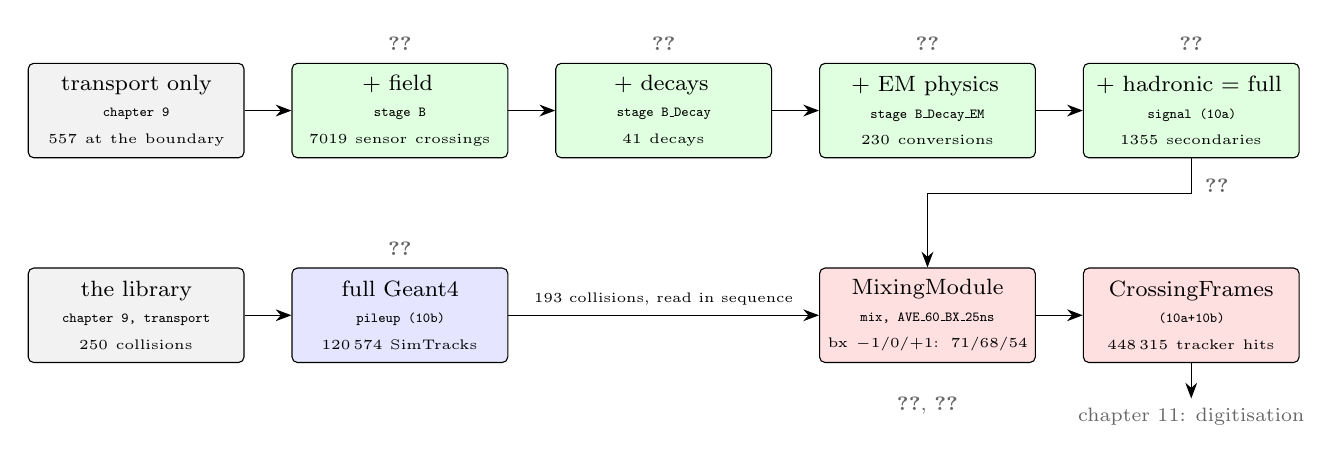
\begin{tikzpicture}[x=1cm, y=1cm, font=\footnotesize, >={Stealth[length=2mm]},
  box/.style={draw, rounded corners=2pt, minimum height=12mm, text width=2.6cm, align=center, inner sep=2pt},
  tr/.style={box, fill=black!5}, sig/.style={box, fill=green!12}, pu/.style={box, fill=blue!10}, mx/.style={box, fill=red!12}]
\node[tr]  (t) at (0,0)    {transport only\\{\tiny\ttfamily chapter 9}\\{\tiny 557 at the boundary}};
\node[sig] (b) at (3.35,0)  {+ field\\{\tiny\ttfamily stage B}\\{\tiny 7019 sensor crossings}};
\node[sig] (d) at (6.7,0)  {+ decays\\{\tiny\ttfamily stage B\_Decay}\\{\tiny 41 decays}};
\node[sig] (e) at (10.05,0)  {+ EM physics\\{\tiny\ttfamily stage B\_Decay\_EM}\\{\tiny 230 conversions}};
\node[sig] (h) at (13.4,0) {+ hadronic = full\\{\tiny\ttfamily signal (10a)}\\{\tiny 1355 secondaries}};
\node[tr]  (l0) at (0,-2.6)   {the library\\{\tiny\ttfamily chapter 9, transport}\\{\tiny 250 collisions}};
\node[pu]  (l)  at (3.35,-2.6) {full Geant4\\{\tiny\ttfamily pileup (10b)}\\{\tiny 120\,574 SimTracks}};
\node[mx]  (m)  at (10.05,-2.6) {MixingModule\\{\tiny\ttfamily mix, AVE\_60\_BX\_25ns}\\{\tiny bx $-1$/0/$+1$: 71/68/54}};
\node[mx]  (c)  at (13.4,-2.6) {CrossingFrames\\{\tiny\ttfamily (10a+10b)}\\{\tiny 448\,315 tracker hits}};
\draw[->] (t) -- (b); \draw[->] (b) -- (d); \draw[->] (d) -- (e); \draw[->] (e) -- (h);
\draw[->] (l0) -- (l); \draw[->] (l) -- node[above, font=\tiny] {193 collisions, read in sequence} (m);
\draw[->] (h.south) -- ++(0,-0.45) -| (m.north); \draw[->] (m) -- (c);
\draw[->] (c.south) -- ++(0,-0.45) node[below, font=\scriptsize, text=black!60] {chapter 11: digitisation};
\foreach \l/\x in {field/3.35, decay/6.7, em/10.05, had/13.4} \node[font=\scriptsize, text=black!60] at (\x,0.85) {\ref*{sec:10_\l}};
\node[font=\scriptsize, text=black!60] at (3.35,-1.75) {\ref*{sec:10_library}};
\node[font=\scriptsize, text=black!60] at (10.05,-3.75) {\ref*{sec:10_mixing}, \ref*{sec:10_pileup}};
\node[font=\scriptsize, text=black!60, anchor=west] at (13.45,-0.95) {\ref*{sec:10_stations}};
\end{tikzpicture}
\caption{The chapter as a chain. Top: the signal run four times on top of the transport-only file of
chapter~\ref{ch:09_G4}, one physics ingredient more each time (process name \code{SIMFULL}, one file per stage);
the last stage is the full \code{SIM} step. Bottom: the 250 library collisions through the same full Geant4, and the
\code{MixingModule}, which overlays 193 of them on the signal. The grey numbers are the subsections of
section~\ref{sec:10_numbers}.}
\label{fig:10_chain}
\end{figure}

\begin{table}[!htb]
\centering\small\setlength{\tabcolsep}{4pt}
\caption{The chapter at a glance: what each subsection of section~\ref{sec:10_numbers} adds to the event, and how
much of it there is in our event (\code{ledger\_10\_SIM.txt}, \code{extras\_10\_SIM.txt}).}
\label{tab:10_glance}
\begin{tabular}{@{}c>{\raggedright\arraybackslash}p{3.0cm}>{\raggedright\arraybackslash}p{5.8cm}>{\raggedright\arraybackslash}p{6.4cm}@{}}
\toprule
 & subsection & what it adds & in our event \\
\midrule
\ref{sec:10_field} & the magnetic field & the charged particles bend; the slow ones spiral & 114 of the 159 charged primaries of the tracker region cannot reach the barrel ECAL; 7019 sensor crossings instead of 6734 \\
\ref{sec:10_decay} & decays in flight & $\pi^\pm$, $K^\pm$, $K^0_S$, $\Lambda$ decay where they happen to & 41 decays, 66 daughters; the $K^0_S$ of the $b$ jet decays 2\,m from the vertex \\
\ref{sec:10_em} & electromagnetic physics & energy loss, conversions, bremsstrahlung, electromagnetic showers & 230 conversions; a $44\GeV$ photon puts two thirds of its shower in one crystal \\
\ref{sec:10_had} & hadronic physics & nuclear interactions, hadronic showers, invisible energy & 385 inelastic interactions; a quarter of the charged hadrons interact in the tracker \\
\ref{sec:10_stations} & the signal station by station & the hits of the full simulation per detector & $10\,272$ tracker hits, $12\,804$ ECAL and 1353 HCAL cells, no muon hit \\
\ref{sec:10_library} & the pileup library & 250 minimum-bias collisions, full physics & library event 72: 2097 tracker hits, $53\GeV$ in the ECAL \\
\ref{sec:10_mixing} & the mixing & 193 collisions in three bunch crossings, shifted in time & $31\,060$ pileup primaries; their vertices spread over $\pm10\cm$ \\
\ref{sec:10_pileup} & where the pileup goes & the hits of the mixture per detector & the signal is 2.3\,\% of the tracker hits; 98\,\% of the barrel crystals are hit \\
\bottomrule
\end{tabular}
\end{table}

Subsections 1 to 4 follow the signal through the four stages. The script runs it four times on top of the
transport-only file (\code{B}, \code{B\_Decay}, \code{B\_Decay\_EM} and the full list, called \code{signal}), and the
\code{SimAnalyzer} pages of each stage show what each ingredient did to the same 571 particles. Each of these
subsections has the same four parts: \emph{what it does} (the physics in plain words), \emph{the parameters} (where
the release sets them), \emph{the numbers of the event}, and a picture. Subsection~5 looks at the full simulation
detector by detector, with the \code{SimHitAnalyzer}. Subsections 6 to 8 are the pileup at the same level: the
library (sample 10b), the mixing, and the mixed event (sample 10a+10b). This is the only place in the book where one
can still see which hit came from which collision; chapter~\ref{ch:11_DIGI} digitises exactly this mixture.

\begin{plainwords}[What Geant4 does with a particle]
Geant4 moves every particle in steps. At each step it asks the physics list which process happens next (a
decay, an interaction, a photon conversion, nothing but a bend in the field) and draws the step length from the
cross sections of the material. A new particle created on the way is a \emph{secondary}; it is tracked in turn,
and kept as a \code{SimTrack} only if it is worth storing (the \code{StackingAction} and the persistency thresholds
of the sensitive detectors decide). When a step is inside a \emph{sensitive detector}, the detector records it:
the tracker and the muon chambers write a \code{PSimHit} per crossing of a sensor (entry and exit point, energy
loss, time of flight, the track that made it); the calorimeters add every energy deposit of a step to a
\code{PCaloHit} per cell and per particle that entered the calorimeter. A hit therefore knows its \emph{primary},
the generator particle that started the chain, and the analyzers colour every hit by the kind of that primary.
Nothing is digitised here: a \code{PCaloHit} is a deposited energy in GeV (in the HF, a number of photoelectrons
of the shower library), not yet a signal of the electronics.
\end{plainwords}

\begin{plainwords}[Which particles are kept: production cuts and persistency]
Two thresholds keep the simulation finite. A \emph{production cut} decides whether a soft secondary is created
at all: an electron or a photon is created only above an energy that Geant4 derives, material by material, from a
range cut, 1\,mm in the ECAL and in the dead material of the tracker, $0.1$\,mm in the strip sensors, $10\,\mu$m
in the pixel sensors, $5\,\mu$m in the photodiodes of the ECAL (the \code{ProdCuts.xml} files of \path{Geometry/*SimData}); below it, the energy is
deposited along the step. A \emph{persistency} rule decides which of the tracked particles are written out: all primaries, the decay
products and conversions of a primary (\code{SaveAllPrimaryDecayProductsAndConversions = True}), a particle that leaves
a tracker hit with more than $0.2\GeV$ (\code{TrackerSD.EnergyThresholdForPersistencyInGeV}) and one that enters a
calorimeter with more than $1\GeV$ (\code{CaloSD.EminTrack}), so that the hits can name it. Everything else is tracked
and forgotten: the thousands of particles of a shower are only in the energy of the hits.
\end{plainwords}

\section{From the previous chapter}

Two files enter (Rule E), both with the process name \code{SIM} of the transport-only Geant4 of
chapter~\ref{ch:09_G4}: the signal, \path{test/09_G4/out/step2_G4_signal_09_G4.root}, 571 primaries of the 634
stable particles with $6923\GeV$ and $471.7\GeV$ of \pt{}, 557 of them reaching the tracker/calorimeter boundary,
6734 tracker crossings with zero energy loss and 459 HF cells of the shower library; and the library,
\path{step2_G4_pileup_09_G4.root}, the 250 collisions, of which library events 72 to 139 are the 68 in-time
collisions with $10\,388$ primaries.\footnote{The numbers of this chapter are in
\path{test/10_SIM/out/ledger_10_SIM.txt} (the output of \code{common/simLedger.py}), in the five
\path{simAnalyzer_<stage>_10_SIM.log}, in \path{simHits_signal_10_SIM.log}, \path{simHits_pileup_10_SIM.log},
\path{simHits_mixed_10_SIM.log} (the latter extracted from the mixing job log \path{step3_MIX_10_SIM.log}) and in
\path{extras_10_SIM.txt} (the FWLite script \path{test/10_SIM/simExtras_10_SIM.py}); the few other ones (time-of-flight
windows, the library totals, the generator status of the pileup primaries) were read with FWLite and are listed in the
companion, section~4.} Every stage reads the signal file again and runs the
\code{SIM} step on it under a new process name, \code{SIMFULL}, with the output command \code{drop *\_*\_*\_SIM}:
the transport-only products are not copied, so each file holds the generator record of
chapters~\ref{ch:06_Decay}--\ref{ch:07_GenJet} and one set of simulation products, those of its own physics. The
hand-over is the same in every stage, 571 primaries from the same smeared vertex $(0.028, -0.017, 3.11)\cm$ and
the same 29 generator vertices; what changes is everything after the first step. The \code{SimHitAnalyzer} counts
$10\,414$ primaries in the 68 in-time collisions, 26 more than chapter~\ref{ch:09_G4}, because it counts every
\code{SimTrack} with a generator link: in the minimum-bias record 25 of those links point at an intermediate
particle (14 gluons, quarks and diquarks of the beam remnants, a $\rho$, a $K^*$) and one is duplicated. The two
objects to follow are unchanged: the $b$ system, 8 of its 9 stable particles handed over, $56.8\GeV$ of \pt{} at
$(\eta,\phi) = (-1.55, -2.09)$ (the $37.5\GeV$ antineutrino is gone), and the $\bar b$ system, 16 of 16,
$114.2\GeV$ at $(-3.75, 1.01)$, pointing at the HF.

Every job of this chapter runs, like chapter~\ref{ch:09_G4}, with the 2025 settings of the release
(\code{auto:phase1\_2025\_realistic}, \code{Run3\_2025}): the geometry and the field map are those of 2024,
and nothing in \code{g4SimHits} or in the \code{MixingModule} depends on the year. The four stages, the library
and the mixture come out as with the 2024 settings, hit for hit, and the mixing draws the same 71, 68 and 54
collisions (companion, section~4). Only the drawing moves: the analyzers place a tracker hit, recorded in the frame
of its module, with the reconstruction geometry, which applies the tracker alignment of the global tag, and the
2025 alignment (\code{TrackerAlignment\_Run3MC\_2025\_EOY\_v1}) puts the modules $10\,\mu$m away from those of
2024 in the median, the TEC $0.3$\,mm: invisible in the displays, and no number of the chapter changes.

\section{The numbers of the event}
\label{sec:10_numbers}

Table~\ref{tab:10_stages} is the ledger of the physics, ingredient by ingredient; subsections~1 to 4 read it line by
line. Two columns run through all of it: the number of primaries that reach the tracker/calorimeter boundary
(\code{CaloTrkProcessing} stores the crossing point and momentum in the \code{SimTrack}; a primary that decays,
converts or interacts before does not count), which falls from 557 to 310, and the $b$ system at that boundary, whose
\pt{} falls from $56.8$ to $24.4\GeV$. Neither number means that energy is lost: it means that more and more of the
energy reaches the calorimeters carried by secondaries.

\begin{table}[htb]
\centering\scriptsize\setlength{\tabcolsep}{2.2pt}
\caption{The Geant4 physics switched on stage by stage, for the signal event (\code{ledger\_10\_SIM.txt}, from the
\code{SimAnalyzer} logs; the first line is the transport-only run of chapter~\ref{ch:09_G4}): primaries reaching
the tracker/calorimeter boundary (of 571), secondaries kept as \code{SimTrack}s by creator process, tracker and
muon-chamber \code{PSimHit}s with their summed energy loss, calorimeter cells with a \code{PCaloHit} and the energy
per subdetector (GeV; HO omitted, at most $0.003\GeV$; HF in photoelectrons of the shower library), and the $b$
system: \pt{} of its primaries at the boundary and its ECAL energy, in GeV.}
\label{tab:10_stages}
\begin{tabular}{lrrrrrrrrrrrrr}
\toprule
stage & boundary & \multicolumn{2}{c}{secondaries} & \multicolumn{2}{c}{\code{PSimHit}s} & $\sum dE$ & cells & EB & EE & HB & HE & HF & $b$: \pt{}, $E_{\rm ECAL}$ \\
 & & all & decay/EM/had & tracker & muon & [GeV] & & & & & & & \\
\midrule
transport (09)        & 557 & 0    & 0/0/0         & 6734   & 0   & 0    & 459    & 0    & 0     & 0    & 0    & 1511 & 56.8, 0 \\
+ field (\code{B})    & 552 & 0    & 0/0/0         & 7019   & 0   & 0    & 454    & 0    & 0     & 0    & 0    & 1533 & 56.6, 0 \\
+ decays              & 507 & 66   & 66/0/0        & 7304   & 0   & 0    & 451    & 0    & 0     & 0    & 0    & 1607 & 48.7, 0 \\
+ EM physics          & 378 & 733  & 67/666/0      & 7339   & 522 & 1.17 & 8467   & 46.8 & 190.5 & 0.15 & 1.34 & 1599 & 26.0, 77.9 \\
+ hadronic (\code{signal}) & 310 & 1355 & 196/773/386 & 10\,272 & 0 & 2.33 & 14\,157 & 68.0 & 293.7 & 0.22 & 1.66 & 1849 & 24.4, 63.6 \\
\bottomrule
\end{tabular}
\end{table}

\subsection{The magnetic field}
\label{sec:10_field}

\textbf{What it does.} A particle of charge $\pm1$ and transverse momentum \pt{} in a field $B$ along the beam
moves on a helix whose projection on the transverse plane is a circle of radius
\[ R\,[\mathrm{m}] = \frac{\pt\,[\mathrm{GeV}]}{0.3\,B\,[\mathrm{T}]} = 0.88\,\mathrm{m}\times\pt\,[\mathrm{GeV}]
\quad\text{at } B=3.8\,\mathrm{T}, \]
while its momentum along the beam is untouched. A track that starts on the beam axis can get no further from it
than the diameter $2R$, so it reaches the front face of the barrel ECAL, at $r=1.29$\,m, only if
$\pt > 0.3\times3.8\times1.29/2 = 0.735\GeV$. Below that it is a \emph{looper}: it circles around the beam while
drifting along it, and leaves the tracker through one of its ends, not through its side. A fast track is only
deflected: at radius $r$ its azimuth has turned by $\sin\Delta\phi = r/2R$, and over the $1.1$\,m of the tracker its
path departs from a straight line by the \emph{sagitta} $s = L^2/8R$. This small curvature, measured by the tracker
to a few tens of micrometres, is how the reconstruction will measure the momentum of a charged particle.

\textbf{The parameters.} The transport-only run of chapter~\ref{ch:09_G4} had \code{UseMagneticField = False};
stage \code{B} switches it on and keeps everything else of that run, the transport-only physics list and
\code{TrackerSD.ZeroEnergyLoss = True}. The field is the map \code{MFGeometry\_160812} at $3.8$\,T of the global tag
(chapter~\ref{ch:09_G4}). Geant4 cannot follow a curved path exactly; it replaces it by chords and checks the error
against the parameters of \code{MagneticField.ConfGlobalMFM} in \path{SimG4Core/Application/python/g4SimHits_cfi.py}:
a chord may miss the true path by $2\,\mu$m (\code{DeltaChord = 0.002} mm; $1\,\mu$m in the tracker), a step ends
within $1\,\mu$m of where it should (\code{DeltaOneStep = 0.001} mm; $0.1\,\mu$m in the tracker), and particles
below $15\MeV$ (\code{EnergyThSimple = 0.015} GeV) are moved with coarser tolerances ($0.1$\,mm).

\textbf{The numbers of the event.} Most charged particles of a $pp$ event are slow. Of the 277 charged primaries of
the signal, 159 are in the tracker region, $\abseta<2.5$, and 114 of those have $\pt<0.735\GeV$, the median being
$0.48\GeV$ (\code{extras\_10\_SIM.txt}, section 1): almost three quarters of the charged particles that the tracker sees can
never reach the barrel calorimeter. In the barrel, $\abseta<1.48$, there are 54 of them, and 53 still reach the
tracker/calorimeter boundary, at the end of the tracker, after spiralling along the beam; that is why the column
``boundary'' of table~\ref{tab:10_stages} hardly moves, 552 instead of 557. The five that are lost are four very
soft pions, $0.03$ to $0.2\GeV$ at $2.5<\abseta<5.3$, which spiral along the beam line and never cross the boundary,
and one $\pi^-$ of $0.45\GeV$ at $\eta=-1.01$. The loopers make themselves seen in the tracker: they cross the same layers several times,
and the sensor crossings grow from 6734 to 7019, 276 of the 285 new ones from the charged primaries below
$0.735\GeV$ (2756 crossings instead of 2480); the neutral primaries make exactly the 3283 crossings they made without
field.

\emph{A worked example: the followed $\pi^+$.} The leading charged hadron of the $b$ jet, the $\pi^+$ that the
\code{SimHitAnalyzer} follows, has $\pt=13.31\GeV$ at $\eta=-1.545$: $R=13.31/(0.3\times3.8)=11.7$\,m. It crosses the
boundary at $r=123.3\cm$, $z=-272.8\cm$, with its azimuth turned by $0.0518$\,rad, $6.4\cm$ along the circle,
against $\arcsin(1.233/(2\times11.7))=0.0528$\,rad for a uniform $3.8$\,T: averaged over its path, the field of
the map is 2\,\% weaker than at the centre. Over $1.1$\,m its sagitta is $1.1^2/(8\times11.7)=1.3\cm$. The $b$
system as a whole arrives with $56.6$ instead of $56.8\GeV$ of \pt{}: the vector sum of eight tracks that no longer
point exactly where they were aimed (figure~\ref{fig:10_field}).

\begin{figure}[!htb]
\centering
\includegraphics[width=0.48\textwidth,trim=0 0 168 0,clip]{10_SIM/out/simAnalyzer_B_10_SIM_page-2.png}\hfill
\includegraphics[width=0.48\textwidth,trim=0 0 168 0,clip]{10_SIM/out/simAnalyzer_B_10_SIM_page-4.png}
\caption{Stage \code{B}, the field alone (\code{simAnalyzer\_B\_10\_SIM\_page-2.png}, \code{\_page-4.png}, the
legend panel cropped). Left: the 552 primaries at the tracker/calorimeter boundary, the grey line of each going back
to its direction at the vertex; open markers, the 19 that do not get there. The $b$ system (red) is at
$(\eta,\phi)=(-1.56,-2.06)$, the $\bar b$ system (blue) at $(-3.75,1.01)$. Right: the 7019 sensor crossings, by
subdetector; the short vertical strings are loopers, crossing the same layer again and again at nearly the same
$\eta$.}
\label{fig:10_field}
\end{figure}

\subsection{Decays in flight}
\label{sec:10_decay}

\textbf{What it does.} Pythia8 decayed every hadron with $c\tau<10\mm$ (chapter~\ref{ch:09_G4}); the long-lived
ones are left to Geant4, which decays them where they happen to decay. A particle of mass $m$, momentum $p$ and
proper lifetime $\tau$ flies on average $\beta\gamma c\tau = (p/m)\,c\tau$ before it decays, and the actual
distance is drawn from an exponential with that mean. The proper decay lengths make the classes: $c\tau=7.8$\,m for
a $\pi^\pm$ and $3.7$\,m for a $K^\pm$ (most of them leave the tracker before decaying), $2.7\cm$ for a $K^0_S$ and
$7.9\cm$ for a $\Lambda$ (at a few GeV they decay inside the tracker, a \emph{displaced vertex} of two tracks). The
daughters are drawn from the decay tables of Geant4; a neutrino daughter is created and killed at once
(\code{TrackNeutrino = False}).

\textbf{The parameters.} Stage \code{B\_Decay} takes the production list, \code{FTFP\_BERT\_EMM}, with its
electromagnetic and hadronic constructors switched off (\code{Physics.EMPhysics = False}, \code{HadPhysics =
False}), so that \code{G4DecayPhysics} is the only process besides the transport; the tracker still records crossings
with zero energy loss.

\textbf{The numbers of the event.} 41 decays leave 66 daughters stored as \code{SimTrack}s (the file
\code{extras\_10\_SIM.txt},
section 2). Twelve pions and three kaons decay to a muon (and an unstored neutrino); ten $K^0_S$ decay, seven to two charged
pions, three to two neutral ones whose $\pi^0$ decay at once to photons (seven $\pi^0\to\gamma\gamma$); seven $\Lambda$ or $\bar\Lambda$ and two
$\bar\Sigma$ decay to a nucleon and a pion. The decay points are spread through the tracker: 10 in the beam pipe, 12
in the pixel volume, 18 among the strips, one in the calorimeters. Every decayed primary stops counting as a primary at the boundary,
which falls from 552 to 507.

\emph{A worked example: the $K^0_S$ of the $b$ jet.} One of the eight primaries of the $b$ system is a $K^0_S$ of
$E=20.6\GeV$ ($\pt=7.96\GeV$). With $m=0.498\GeV$, $\beta\gamma=41$ and its mean flight is $41\times2.68\cm=1.1$\,m.
It decayed at $r=80.2\cm$, $z=-188.5\cm$, $2.08$\,m from the vertex, almost two mean flights (a 15\,\% chance),
among the endcap disks of the tracker, into $\pi^+\pi^-$ (figure~\ref{fig:10_decay}, the two red markers). The $b$
system reaches the boundary with 7 of its 8 primaries and $48.7\GeV$ instead of $56.6$: the two pions carry the rest,
but as secondaries.

\begin{figure}[!htb]
\centering
\includegraphics[width=0.54\textwidth,trim=0 0 168 0,clip]{10_SIM/out/simAnalyzer_B_Decay_10_SIM_page-3.png}
\caption{Stage \code{B\_Decay} (\code{simAnalyzer\_B\_Decay\_10\_SIM\_page-3.png}, legend cropped): the 66 secondaries,
all decay products, at the direction of their production; marker size grows with \pt{}. Red: the two pions of the
$K^0_S$ of the $b$ system, $7.96\GeV$ of \pt{} together. The grey dots are the primaries.}
\label{fig:10_decay}
\end{figure}

\subsection{Electromagnetic physics}
\label{sec:10_em}

\textbf{What it does.} Five processes act on charged particles and photons. \emph{Ionisation}: a charged particle
loses energy to the electrons of the material, continuously, and now and then knocks one out with enough energy to
be a particle of its own (a $\delta$ ray). \emph{Multiple scattering}: many small deflections by the nuclei, which
blur the direction. \emph{Bremsstrahlung}: an electron radiates a photon in the field of a nucleus. \emph{Pair
production}: a photon converts into an $e^+e^-$ pair, also in the field of a nucleus. \emph{Compton scattering} of a
photon on an electron, and at the lowest energies the photoelectric effect. The first two give the tracker hits their
energy loss and the tracks their wiggles; the last three, in dense material, build the electromagnetic shower.

\begin{plainwords}[Radiation length, shower, Moli\`ere radius]
The \emph{radiation length} $X_0$ of a material is the distance over which an electron keeps $1/e$ of its energy to
bremsstrahlung; a high-energy photon converts after $\frac97X_0$ on average, so that a slab of $t$ radiation lengths
converts a fraction $1-e^{-7t/9}$ of the photons. A photon or electron of energy $E$ entering a dense material starts
a cascade: every $X_0$ or so the number of particles doubles and their energy halves, until the energy per
particle reaches the \emph{critical energy} $E_c$, where ionisation wins and the shower dies out. The maximum is
at a depth of about $\ln(E/E_c)\,X_0$, and the shower is narrow: 90\,\% of its energy is inside a cylinder of one
\emph{Moli\`ere radius} $R_M$. For the lead tungstate of the ECAL, $X_0=0.89\cm$, $R_M\approx2\cm$, $E_c\approx9\MeV$:
a crystal, 22 to $23\cm$ long (about $25X_0$) and $2.2\cm$ wide in the barrel ($2.9\cm$ in the endcap), contains a
shower in depth and catches most of it across in itself and its neighbours. For a $44\GeV$ photon the maximum is
$\ln(44\,000/9)\approx8.5$ radiation lengths, $7.5\cm$, deep.
\end{plainwords}

\textbf{The parameters.} Stage \code{B\_Decay\_EM} adds \code{EMPhysics = True} to the previous stage and lets the
tracker record the energy loss (\code{ZeroEnergyLoss} back to its default, \code{False}); the constructor is the CMS
one, \code{CMSEmStandardPhysics} of \code{FTFP\_BERT\_EMM} (chapter~\ref{ch:09_G4}). The production cuts of the box
above apply from here on; particles are tracked down to \code{G4TrackingCut = 0.025}\,MeV, and the ECAL keeps a
\code{PCaloHit} only above $15\MeV$ in the barrel and $10\MeV$ in the endcap (\code{CaloSD.EminHits}).

\textbf{The numbers of the event.} The stage creates 666 secondaries (\code{extras\_10\_SIM.txt}, section 3): 430
electrons and positrons of 230 conversions, 213 bremsstrahlung photons, 20 $\delta$ rays and 3 Compton electrons. The
conversions are where the material is: one in the beam pipe, 16 in the pixel volume, 121 among the strips, 41
between the tracker and the calorimeters, 4 in the preshower, and 47 in the calorimeters themselves, where the photons
that crossed the tracker begin their showers (the conversion of a primary photon is stored wherever it happens; 187
of the 230 are of a primary photon). Of the 29 primary photons of more than $1\GeV$ in $\abseta<2.5$, 18 converted
inside the tracker in this stage and 15 in the full simulation, the point of a conversion being a random draw: with
$1-e^{-7t/9}=15/29$ to $18/29$, the photons of this event crossed on average $t\approx0.9$ to $1.2\,X_0$ of tracker
material, a rough estimate from 29 photons, 26 of them at $1<\abseta<2.5$. The tracker and muon hits now carry an
energy loss, $1.17\GeV$ in all, $0.15\MeV$ per crossing on average ($0.23\MeV$ in the full simulation; a
minimum-ionising particle loses $0.12\MeV$ in $300\,\mu$m of silicon, slow particles and $\delta$ rays more). The calorimeters fill: 8467 cells, $46.8\GeV$ in the EB and $190.5\GeV$ in the EE. Two things are odd in
this stage, and both are the missing hadronic physics: 522 muon-chamber hits (DT 7, CSC 448, RPC 30, GEM 37) from
charged hadrons that crossed the calorimeters like heavy muons, ionising all the way, and $0.15\GeV$ in the HB, their
ionisation in 52 HB cells on the way out. The $b$ system deposits $77.9\GeV$ in the ECAL, more than it will
in the full simulation.

\emph{A worked example: one photon, two showers.} The photon of highest \pt{} that the \code{SimHitAnalyzer}
follows belongs to the $b$ jet: $E=44.27\GeV$, $\pt=17.73\GeV$, $\eta=-1.566$, aimed at the endcap ECAL.
Table~\ref{tab:10_photon} compares where its energy went in this stage and in the full simulation; the physics of a
photon is the same in both, only the random numbers differ. Here it crossed the whole tracker unconverted and
converted at $r=112\cm$, $z=-254\cm$, just behind it, in front of the endcap: a textbook shower, 97\,\% of its energy in the
crystals, two thirds in one crystal, 90\,\% in six. In the full simulation it converted at $r=3.0\cm$, in the first
pixel layer. The electron and the positron then crossed $1$\,m of tracker in the field: they were bent apart in
$\phi$, radiated bremsstrahlung photons in the material, and left 171 tracker hits on the way. What reached the ECAL
was a spray: 466 crystals, the hottest with a fifth of the energy, 90\,\% in 38 crystals, and 11\,\% that never
reached a crystal. Same photon, same calorimeter: the tracker material in front decided the shape, and the
reconstruction will have to collect the energy along $\phi$, where the field spread it.

\begin{table}[!htb]
\centering\small
\caption{The followed photon of the $b$ jet ($E=44.27\GeV$, $\eta=-1.566$), its own deposits in the barrel and endcap
crystals in two runs (\code{extras\_10\_SIM.txt}, section 6). In brackets: the fraction of its energy (third line),
of its deposits (below).}
\label{tab:10_photon}
\begin{tabular}{@{}lrr@{}}
\toprule
 & stage \code{B\_Decay\_EM} & full simulation (\code{signal}) \\
\midrule
converts at & $r=112\cm$, $z=-254\cm$ & $r=3.0\cm$, $z=-3.7\cm$ \\
tracker hits of its descendants & 0 & 171 \\
crystals with energy, energy in them & 156, $42.79\GeV$ (97\,\%) & 466, $39.45\GeV$ (89\,\%) \\
the hottest crystal & $28.57\GeV$ (67\,\%) & $7.80\GeV$ (20\,\%) \\
the five hottest & $38.11\GeV$ (89\,\%) & $18.56\GeV$ (47\,\%) \\
90\,\% of its deposits in & 6 crystals & 38 crystals \\
\bottomrule
\end{tabular}
\end{table}

\begin{figure}[!htb]
\centering
\includegraphics[width=0.48\textwidth,trim=0 0 168 0,clip]{10_SIM/out/simAnalyzer_B_Decay_EM_10_SIM_page-3.png}\hfill
\includegraphics[width=0.48\textwidth,trim=0 0 168 0,clip]{10_SIM/out/simAnalyzer_B_Decay_EM_10_SIM_page-5.png}
\caption{Stage \code{B\_Decay\_EM} (\code{simAnalyzer\_B\_Decay\_EM\_10\_SIM\_page-3.png}, \code{\_page-5.png}, legends
cropped). Left: the 733 secondaries by creator process, green squares the conversions, orange triangles the
bremsstrahlung photons, purple the decays; red, the 49 of the $b$ system. Right: the 8467 calorimeter cells, size
growing with the energy; the $b$ system (red, $77.9\GeV$) is a dense block of EE crystals at $(-1.6,-2.1)$, the
$\bar b$ system (blue) a block of HF cells at $\eta=-3.75$. The EB and EE are full of small isolated deposits: the
photons of the event, each a small shower.}
\label{fig:10_em}
\end{figure}

\subsection{Hadronic physics}
\label{sec:10_had}

\textbf{What it does.} A hadron also feels the nuclei through the strong force. In an \emph{elastic} collision it
is only deflected. In an \emph{inelastic} one the nucleus breaks up: new pions, protons, neutrons and nuclear
fragments come out, each of which can interact again, a \emph{hadronic shower}. It differs from an electromagnetic
one in three ways. It is longer and wider. A part of it is electromagnetic: the $\pi^0$ produced in the interactions
decay at once into two photons, which shower like any photon, and how large that part is fluctuates from one shower
to the next. And a part of the energy is \emph{invisible}: it goes into breaking nuclei (binding energy), into slow
neutrons and into neutrinos, and no sensitive volume ever sees it. A calorimeter therefore answers less to a hadron
than to an electron of the same energy.

\begin{plainwords}[Interaction length and sampling]
The \emph{nuclear interaction length} $\lambda_I$ is the mean free path of a hadron before an inelastic
interaction: about $20\cm$ in lead tungstate and $16\cm$ in brass, twenty times the radiation length. An ECAL crystal
is about one $\lambda_I$ deep: two hadrons in three start their shower already in the ECAL, and the rest of the
shower develops in the HCAL behind it. The HB and HE are \emph{sampling} calorimeters: brass absorber plates with
thin plastic scintillator tiles in between, and only the scintillator is sensitive. A \code{PCaloHit} of the HCAL is
the energy deposited in the scintillator, after the Birks law that describes how the light of a scintillator
saturates for densely ionising particles (\code{HCalSD.UseBirkLaw}), a few per cent of the energy of the shower. The
digitisation of chapter~\ref{ch:11_DIGI} multiplies it back by a \emph{sampling factor}, about 125 in the HB and 186
to 211 in the HE.
\end{plainwords}

\textbf{The parameters.} The stage \code{signal} adds \code{HadPhysics = True}: the full list \code{FTFP\_BERT\_EMM}
of the production. Its hadronic part is two models joined in energy: the Bertini intranuclear cascade (\code{BERT})
for slow hadrons, the Fritiof string model followed by a precompound nuclear de-excitation (\code{FTFP}) for fast ones;
between \code{EminFTFP = 3} and \code{EmaxBERT = 6}\,GeV (12 for pions, \code{EmaxBERTpi}) the two are mixed
(\path{g4SimHits_cfi.py}, \path{SimG4Core/PhysicsLists/plugins/FTFPCMS_BERT_EMM.cc}).

\textbf{The numbers of the event.} 385 inelastic and one elastic nuclear interaction; the 1355 secondaries sit in 768
\code{SimVertex}s. The decays rise from 67 to 196: the interactions make new unstable particles, the $\pi^0$ among
them, whose photons shower and convert (773 electromagnetic secondaries). The stored hadronic secondaries are those of interactions in or near
the tracker (\code{extras\_10\_SIM.txt}, section 4): 142 interaction vertices, 4 in the beam pipe, 13 in the pixel
volume, 85 among the strips, 26 between the tracker and the calorimeters, 14 in the preshower and the calorimeters,
producing 178 charged pions, 62 $\pi^0$, 60 neutrons and 58 protons, from 102 charged pions,
10 protons, 10 neutrons and a few kaons. A quarter of the charged hadrons interact before the calorimeter: of the 73
primary charged pions, kaons and protons with $\pt>0.5\GeV$ in $\abseta<2.5$, 19 (26\,\%) have a nuclear interaction
inside the tracker, as if the tracker were $0.3\,\lambda_I$ thick for them. The interactions in the calorimeters are
there too, but only in the energy of the cells (box ``Which particles are kept''). The tracker has 2933 hits more than in the EM stage, $10\,272$, 2232 of them from tracks not stored as
\code{SimTrack}s: the soft products of the nuclear interactions in the pixel and strip material. The muon chambers
are empty again, the hadrons being absorbed in the calorimeters; the HB and HE hold $0.22$ and $1.66\GeV$ of visible
energy. Only 310 primaries reach the boundary intact (figure~\ref{fig:10_stage}).

\emph{A worked example: where the energy of the $b$ jet goes.} Table~\ref{tab:10_bbudget} follows the eight
primaries of the $b$ system, $140.3\GeV$ of energy, into the calorimeters. The ECAL holds $63.6\GeV$, less than with
EM physics alone ($77.9\GeV$): the two charged pions of $32.6$ and $26.6\GeV$ now interact instead of crossing it like
muons, and much of their energy goes into the HCAL, into neutrons and nuclear fragments. The HCAL holds $0.386\GeV$ of
visible energy in 122 cells, nearly all in the HE. Multiplied by the sampling factors of chapter~\ref{ch:11_DIGI},
about 125 and 190, that is some $72\GeV$: the two calorimeters together give back roughly the $140\GeV$ of the jet,
half in each, the closeness of the sum being partly luck, since a sampling factor is an average over showers. The
$\bar b$ jet, $2421\GeV$ in 16 primaries at $\eta=-3.75$, puts $9.9\GeV$ into the ECAL on its way ($9.4\GeV$ in
the edge of the EE) and 987 photoelectrons into the HF.

\begin{table}[!htb]
\centering\small
\caption{The $b$ system in the full simulation: its primaries and their calorimeter deposits
(\code{extras\_10\_SIM.txt}, section 5; the hits are attributed to the primary through the \code{SimTrack} and
\code{SimVertex} parents, as the analyzers do). The antineutrino, $95.5\GeV$, was not handed over
(chapter~\ref{ch:09_G4}).}
\label{tab:10_bbudget}
\begin{tabular}{@{}ll@{}}
\toprule
the 8 primaries, energy in GeV & $\gamma$ 44.3, $\pi^\pm$ 32.6, $\pi^\pm$ 26.6, $K^0_S$ 20.6, $e^-$ 10.9, $\gamma$ 4.1, 0.8, 0.4 \\
handed to Geant4 & $140.3\GeV$ \\
reaching the boundary as primaries & 3 of 8, $\pt=24.4\GeV$ \\
\midrule
ECAL: EB, EE, ES & $6.23\GeV$ (364 crystals), $57.32\GeV$ (895), $0.02\GeV$ (96 strips) \\
ECAL, total & $63.58\GeV$ \\
HCAL visible: HB, HE & $0.010\GeV$ (17 cells), $0.376\GeV$ (105 cells) \\
HCAL $\times$ sampling factor (chapter~\ref{ch:11_DIGI}) & $\approx 0.010\times125+0.376\times190\approx72\GeV$ \\
\bottomrule
\end{tabular}
\end{table}

\begin{figure}[!htb]
\centering
\begin{subfigure}[t]{0.495\textwidth}
\includegraphics[width=\textwidth]{10_SIM/out/simAnalyzer_signal_10_SIM_page-08.png}
\caption{the 1355 secondaries by creator process: 196 decays, 773 electromagnetic (488 conversions, 275
bremsstrahlung), 386 hadronic; red: the $b$ system (133), blue: the $\bar b$ system (89).}
\end{subfigure}\hfill
\begin{subfigure}[t]{0.495\textwidth}
\includegraphics[width=\textwidth]{10_SIM/out/simAnalyzer_signal_10_SIM_page-10.png}
\caption{the $26\,793$ \code{PCaloHit}s summed in $14\,157$ cells, marker size growing with the energy; red: the
1452 cells of the $b$ system ($63.6\GeV$ in the ECAL), blue: the 671 of the $\bar b$ system (987 HF units).}
\end{subfigure}
\caption{The signal through the full Geant4 physics, pages 8 and 10 of \code{simAnalyzer\_signal\_10\_SIM.pdf}
(\code{\_page-08.png}, \code{\_page-10.png}); pages 1--5 are the generator stages, 6 the primaries, 7 the boundary
crossing, 9 the tracker hits. The $b$ jet at $(\eta,\phi)=(-1.55,-2.09)$ is a dense block of conversions and
ECAL cells; the $\bar b$ jet at $\eta=-3.75$ is a block of HF cells.}
\label{fig:10_stage}
\end{figure}

\FloatBarrier
\subsection{The signal station by station}
\label{sec:10_stations}

\textbf{What it shows.} The \code{SimHitAnalyzer} takes the full simulation detector by detector (``stations'':
tracker, ECAL, HCAL, muon system) and draws every hit at its place in the detector, in $r$--$z$, in $x$--$y$ and in
$\eta$--$\phi$, coloured by the kind of the primary it descends from. For the leading primary of every kind it joins
the hits in time order and labels them, so that one particle can be followed through the layers
(figure~\ref{fig:10_stations}): the $\pi^+$ of $13.3\GeV$ of \pt{} of the $b$ jet, the photon of
subsection~\ref{sec:10_em}, the one electron of the event ($\pt=5.0\GeV$, $E=10.95\GeV$), and in the forward
direction a $K^0_S$ of $15.7\GeV$ and a $\pi^+$ of $30.6\GeV$ of the $\bar b$ jet. The $K^0_S$ ($E=338.5\GeV$,
$\eta=-3.77$) flies outside the acceptance of the tracker, but it hits a nucleus of the wall of the beam pipe at
$r=2.2\cm$, $z=-43.7\cm$ (\code{extras\_10\_SIM.txt}, section 4), and the products of that interaction spray 203
hits into the tracker endcap.

\textbf{The numbers of the event} (\code{simHits\_signal\_10\_SIM.log}). The \emph{tracker} has $10\,272$
\code{PSimHit}s (PXB 929, PXF 973, TIB 1182, TID 975, TOB 1022, TEC 5191) from 293 of the 571 primaries. The TEC holds
half of them, both jets being in the endcap directions, and the barrel layers count fewer hits the further out they
are (PXB 397, 221, 179, 132 from layer 1 to 4; TOB 427 to 77): a barrel layer of the same length covers a smaller
range of $\eta$ the larger its radius. By kind, 4999 hits descend from charged hadrons, 890 from neutral hadrons,
2013 from photons (the conversion pairs; 171 from the followed photon alone), 138 from the one electron, 2232 from
tracks without a stored ancestor. $10\,063$ are in the \code{LowTof} collections and
209 in \code{HighTof} ($36$--$499\ns$ after the collision: loopers and slow secondaries). The \emph{ECAL} has $24\,262$
hits in $12\,804$ cells (EB 5521, EE 6214, ES 1069) from 366 primaries: $162\GeV$ in 5287 cells dominated by photons,
$144\GeV$ in 5343 by charged hadrons, $47.4\GeV$ by neutral hadrons, $7.1\GeV$ by electrons; the followed photon
dominates 270 cells with $42.0\GeV$ and the followed $\pi^+$ 35 cells with $3.4\GeV$, a hadron that crossed the
crystals without showering. Of the 7273 EB hits, 1862 ($3.3\GeV$ of the 68) come later than $25\ns$, the slow tail of
the hadronic showers. The \emph{HCAL} has 2531 hits in 1353 cells (HB 173, HE 648, HO 1, HF 531) from 266 primaries;
the HF $\pi^+$ of the $\bar b$ jet alone puts 809 of the 1849 photoelectrons into 19 HF cells. The \emph{muon
chambers} have nothing: no particle of the signal reached them. In all, 512 of the 571 primaries left a hit; the 59
others are neutrals that neither converted nor interacted, and forward particles beside the calorimeters.

\begin{figure}[!htbp]
\centering
\includegraphics[width=0.475\textwidth,trim=0 0 288 0,clip]{10_SIM/out/signal/TRK/simHits_signal_10_SIM_TRK_rz_run1_event1.png}\hfill
\includegraphics[width=0.475\textwidth,trim=0 0 288 0,clip]{10_SIM/out/signal/TRK/simHits_signal_10_SIM_TRK_xy_run1_event1.png}\\[3pt]
\includegraphics[width=0.475\textwidth,trim=0 0 288 0,clip]{10_SIM/out/signal/ECAL/simHits_signal_10_SIM_ECAL_rz_run1_event1.png}\hfill
\includegraphics[width=0.475\textwidth,trim=0 0 288 0,clip]{10_SIM/out/signal/HCAL/simHits_signal_10_SIM_HCAL_rz_run1_event1.png}
\caption{(10a) The signal station by station, legends cropped. Top: the tracker in $r$--$z$ and, for its barrel, in $x$--$y$; bottom: the ECAL and the HCAL in
$r$--$z$. Black: hits of charged hadrons, purple: neutral hadrons, green: photons, orange: electrons, grey: no stored
ancestor; grey dots and frames: the detector elements. The followed primaries are joined in time order and labelled:
the conversion pair of the photon (green) and the electron (orange) cross the whole tracker towards the endcap at
$z\approx-300\cm$; the products of the nuclear interaction of the $K^0_S$ in the beam pipe (purple) fan out into the TID and TEC; in the HCAL the $b$ jet reaches the HE
around $z=-400\cm$ and the $\bar b$ jet the HF at $z=-1115\cm$.
Files: \code{signal/<station>/}\allowbreak\code{simHits\_signal\_10\_SIM\_<station>\_<view>\_run1\_event1.png}.}
\label{fig:10_stations}
\end{figure}

\subsection{The pileup library and one collision}
\label{sec:10_library}

\textbf{What it is.} The library (sample 10b) is the 250 minimum-bias collisions of chapter~\ref{ch:08_PU}, handed
over in chapter~\ref{ch:09_G4}, through the same full Geant4 with its own random seed (\code{PUSEED}$+2 = 20243$). It
is simulated once, independently of the signal, and any number of signal events could take their pileup from it.

\textbf{The numbers of the event.} The 250 collisions give $38\,862$ primaries, which become $120\,574$
\code{SimTrack}s with $548\,028$ tracker hits, $394\,627$ EB hits ($3149\GeV$), $691\,000$ EE hits ($11\,616\GeV$) and
$119\,964$ HCAL hits, 60\,MB in all; they took 7 to 12 minutes, $1.8$ to $2.8$\,s each, the signal event alone 8 to
12\,s, depending on the load of the shared machine. Library event 72, the first in-time collision, has 164 primaries
and 534 \code{SimTrack}s, 2097 tracker hits, 4742 ECAL hits in 3388 cells (EB 1217 cells with $9.45\GeV$, EE 1948
with $43.5\GeV$, ES 223), 392 HCAL hits in 262 cells (HB 21, HE 122, HF 119 with 173 photoelectrons) and 11 CSC hits
in station 1 from a track without stored ancestor; 142 of its 164 primaries left a hit. The collision is a fifth of
the signal in tracker hits and a seventh in ECAL energy ($53$ against $362\GeV$), and its ECAL energy is mostly
charged hadrons ($29.4\GeV$) and photons ($15.7\GeV$) of a few GeV each, spread over the whole detector. Three
diffractive collisions (library events 12, 124, 179) give Geant4 nothing but protons of $6800\GeV$ (one of
$5539\GeV$) at $z=\pm203$\,m: the beam-line transport of the generator step (\code{LHCTransport}, read since
\code{run3\_common} sets \code{g4SimHits.LHCTransport = True}) delivers them to the start of the forward proton
spectrometer (\code{PPSRegionStart = 203}, \path{SimTransport/PPSProtonTransport/python/CommonParameters_cfi.py}).

\begin{plainwords}[The library, and what the production calls the premixing library]
\code{step2\_SIM\_pileup\_10\_SIM.root} is a GEN-SIM library: minimum-bias collisions simulated once, to be overlaid
on any number of signal events. Reading it, 193 collisions per signal event here and about 1000 in the Run-3 production scenario
(section~\ref{sec:10_phase2}), is why the production does not mix SimHits. Its \emph{premixing library} (\code{premix\_stage1}) is made by a job that mixes a full bunch-crossing
train of minimum-bias collisions from a GEN-SIM library like this one and \emph{digitises} it, storing one premixed
event, digis and all, per future signal event (data tier \code{PREMIX}); the signal job then digitises the signal
alone and adds one premixed event to it, channel by channel (\code{premix\_stage2}, the \code{PreMixingModule},
chapter~\ref{ch:11_DIGI}). This chapter stops one step earlier, at the SimHits of the library, because only there
can the hits of the signal and of each collision still be told apart.
\end{plainwords}

\subsection{The mixing}
\label{sec:10_mixing}

\textbf{What it does.} The detector does not see one collision at a time. Every 25\,ns two bunches cross and about
sixty collisions happen at once, at different points along the beam, and a detector whose signal lasts longer than
25\,ns also still sees the collisions of the crossings before and after. The \code{MixingModule} builds that
situation for every signal event. It draws the number of collisions of each bunch crossing, takes that many from the
library, moves each to its bunch crossing by shifting the times of its \code{SimTrack}s, \code{SimVertex}s and hits by
$25\ns\times\bx$, stamps every object with its bunch crossing and its collision (the \code{EncodedEventId}), and lays
everything out in one \code{CrossingFrame} per collection, the signal objects first and the pileup behind them. Each
collision keeps its own vertex, drawn in chapter~\ref{ch:08_PU} from the same luminous region as the signal. The
digitisers of chapter~\ref{ch:11_DIGI} read the \code{CrossingFrame}s, not the signal collections.

\textbf{The parameters.} \code{process.mix} of \code{cmsDriver.py -s DIGI} with the option
\code{--pileup} \code{AVE\_60\_BX\_25ns,\{'N':~60,~'B':~(-1,~1)\}}: a Poisson draw of mean 60 per bunch crossing, three
bunch crossings, 25\,ns apart, the library read in sequence (\code{input.sequential = True}), the random engine of
the module seeded with 12345. The job (\path{python/mixOnly_cff.py}) removes the digitisers and puts the
\code{SimHitAnalyzer} on the \code{CrossingFrame}s.

\textbf{The numbers of the event.} The draw gave 71, 68 and 54 collisions for $\bx=-1$, 0 and $+1$, library events
1--71, 72--139 and 140--193 in that order, and the script checks that the in-time ones are those that chapters
\ref{ch:08_PU} and \ref{ch:09_G4} assumed. The 193 collisions bring $31\,060$ primaries ($10\,012$, $10\,414$,
$10\,634$ by bunch crossing) and $97\,276$ \code{SimTrack}s. They are very unequal: from 1 primary (the PPS protons
above) to 574, with a median of 69, 126 and 154 per collision in the three bunch crossings (\code{extras\_10\_SIM.txt},
section 7); the 54 late collisions happen to be the busiest. Their vertices spread along the beam with an r.m.s. of
$3.76\cm$, from $z=-9.5$ to $+10.1\cm$; two of the 190 vertices near the centre are within 1\,mm of the signal vertex
at $z=3.11\cm$.

\begin{plainwords}[Why the DIGI job of the next chapter replays this draw]
The number of collisions per bunch crossing is a Poisson draw with mean 60 from the random engine of the module
\code{mix} (seed 12345), and the library is read in sequence, so the draw decides which library events are in time:
72--139 here, the \code{SKIP = 71}, \code{NPU = 68} that chapters \ref{ch:08_PU} and \ref{ch:09_G4} used (the
script checks it). The same module with the same seed \emph{with} the digitisers gives other numbers (65, 67 and 56
were observed): \code{BMixingModule::produce} (\path{Mixing/Base/src/BMixingModule.cc}) calls
\code{initializeEvent}, \code{addSignals}, \code{doPileUp} in that order, and \code{addSignals} runs the
digitisers on the signal, which consume random numbers of the same engine before \code{PileUp::CalculatePileup}
(\path{Mixing/Base/src/PileUp.cc}, called from \path{SimGeneral/MixingModule/plugins/MixingModule.cc}) draws
the collisions. The mixing job therefore writes \path{step3_MIX_10_SIM.root}: the signal event again (the
\code{CrossingFrame}s are transient, \code{drop *\_mix\_*\_*}) plus the \code{CrossingFramePlaybackInfoNew} of
the module \code{mix}, process \code{MIX}: which library events went into which bunch crossing.
Chapter~\ref{ch:11_DIGI} reads it with \code{process.mix.playback = True} and digitises exactly these 193 collisions.
\end{plainwords}

\subsection{Where the pileup goes}
\label{sec:10_pileup}

\textbf{The numbers of the event} (\code{simHits\_mixed\_10\_SIM.log}, figure~\ref{fig:10_pileup}). In the
\emph{tracker} the 193 collisions put $438\,043$ hits next to the $10\,272$ of the signal: $139\,551$ early,
$146\,028$ in time, $152\,464$ late, that is 1965, 2147 and 2823 per collision; the signal is 2.3\,\% of the tracker
hits of its own bunch crossing. The innermost pixel layer has $19\,053$ hits, of which 397 are the signal's. In the
\emph{ECAL} they hit nearly every crystal: $59\,897$ of the $61\,200$ of the barrel and $14\,619$ of the $14\,648$
of the endcaps have a hit, and $31\,654$ of the $137\,216$ preshower strips. The 193 collisions dominate $103\,808$
cells with $12\,130\GeV$ ($3950$, $3860$, $4320\GeV$ by bunch crossing, $57\GeV$ per in-time collision) against the
$12\,804$ cells and $362\GeV$ of the signal alone; the endcap crystals alone hold $9720\GeV$, 33 times the signal's
$294$. With the pileup on top, only 2362 cells are still dominated by the signal, holding $236\GeV$; the other
$10\,442$ cells of its showers now belong, by energy, to a pileup particle. The followed photon still dominates 80
crystals with $42.6\GeV$ (270 alone), the followed $\pi^+$ 8 with $3.9\GeV$ (35 alone): the core of a shower
survives, its edges are lost. The \emph{HCAL} goes from 1353 to $11\,021$ cells (HB 3624 of 9072, HE 4170, HO 15, HF
3212 of 3456), 258 of them dominated by the signal; in the HF the drawing shows many cells dominated by the early
collisions (figure~\ref{fig:10_pileup}, olive). The \emph{muon chambers}, empty for the signal, have 204 hits (DT 43, CSC 151, RPC 2,
GEM 8): 51 from the early bunch crossing, 129 in time, 24 late. Of the 571 signal primaries, 378 still own a hit or a
cell in the mixture, down from 512; in the HCAL only 92 of 266, because the cells of the hadronic showers are shallow
and a pileup deposit easily outweighs them.

\begin{figure}[!htbp]
\centering
\includegraphics[width=0.475\textwidth,trim=0 0 288 0,clip]{10_SIM/out/mixed/TRK/simHits_mixed_10_SIM_TRK_xy_run1_event1.png}\hfill
\includegraphics[width=0.475\textwidth,trim=0 0 288 0,clip]{10_SIM/out/mixed/ECAL/simHits_mixed_10_SIM_ECAL_etaphi_run1_event1.png}\\[3pt]
\includegraphics[width=0.475\textwidth,trim=0 0 288 0,clip]{10_SIM/out/mixed/HCAL/simHits_mixed_10_SIM_HCAL_rz_run1_event1.png}\hfill
\includegraphics[width=0.475\textwidth,trim=0 0 288 0,clip]{10_SIM/out/mixed/MUON/simHits_mixed_10_SIM_MUON_rz_run1_event1.png}
\caption{(10a+10b) The mixed event station by station, legends cropped: the tracker barrel in $x$--$y$, the ECAL in $\eta$--$\phi$, the HCAL and the muon system in $r$--$z$.
The signal is drawn as in figure~\ref{fig:10_stations}, the pileup underneath by bunch crossing: olive $-1$, blue 0,
red $+1$; a calorimeter cell takes the colour of the origin that deposited most of its energy. The signal survives as
the black and green dots along the followed tracks and as the core of the $b$ jet at $(-1.6,-2.1)$ in the ECAL; the
204 muon hits are all pileup.
Files: \code{mixed/<station>/}\allowbreak\code{simHits\_mixed\_10\_SIM\_<station>\_<view>\_run1\_event1.png}.}
\label{fig:10_pileup}
\end{figure}

\section{Ledger and display}

Table~\ref{tab:10_ledger} is the ledger of the stage at the level of the hits, for the three samples. For the
signal the stage turns 571 primaries into 1926 \code{SimTrack}s, $10\,272$ tracker hits with $2.33\GeV$ of energy
loss and $26\,793$ calorimeter hits in $14\,157$ cells: $362\GeV$ in the ECAL, $1.9\GeV$ of visible energy in the
HB and HE, 1849 photoelectrons in the HF (the 1851
``GeV'' of the HCAL line are these two added). Of the
$6923\GeV$ handed to Geant4 this is what the sensitive volumes record; the rest is the sampling of the HCAL (its
visible energy is a few per cent of what it absorbs), nuclear binding energy, the
neutrons and neutrinos of the showers, the dead material and the forward particles beyond the HF. For the mixture
the stage adds, on top of the signal, $438\,043$ tracker hits, 204 muon-chamber hits, $103\,808$ ECAL cells with
$12\,130\GeV$ and $10\,763$ HCAL cells; the 68 in-time collisions alone, handed over in chapter~\ref{ch:09_G4}
with $4486\GeV$ of \pt{}, put $146\,028$ tracker hits and $3860\GeV$ of ECAL energy next to the signal's
$10\,272$ and $362$.

\begin{table}[htb]
\centering\scriptsize\setlength{\tabcolsep}{3pt}
\caption{The ledger of the SimHits, station by station (\code{ledger\_10\_SIM.txt}, from the \code{SimHitAnalyzer}
logs): the signal alone (10a), library event~72 alone (10b), and the mixed event (10a+10b) split by origin: the
signal, the 71 collisions of bunch crossing $-1$, the 68 of bunch crossing 0, the 54 of bunch crossing $+1$. A
cell of the mixed event is attributed to the origin that deposited most of its energy. ECAL energies in GeV; the
HCAL ``energy'' is the visible GeV of HB, HE and HO plus the photoelectrons of the HF, as the analyzer sums them.}
\label{tab:10_ledger}
\begin{tabular}{lrrrrrrr}
\toprule
 & (10a) & (10b) & \multicolumn{5}{c}{(10a+10b) the mixed event} \\
\cmidrule(lr){4-8}
 & signal & event 72 & all & signal & early (71) & in time (68) & late (54) \\
\midrule
primaries & 571 & 164 & 31\,631 & 571 & 10\,012 & 10\,414 & 10\,634 \\
\code{SimTrack}s & 1926 & 534 & 99\,202 & 1926 & \multicolumn{3}{c}{97\,276} \\
tracker \code{PSimHit}s & 10\,272 & 2097 & 448\,315 & 10\,272 & 139\,551 & 146\,028 & 152\,464 \\
muon \code{PSimHit}s & 0 & 11 & 204 & 0 & 51 & 129 & 24 \\
ECAL cells & 12\,804 & 3388 & 106\,170 & 2362 & 32\,941 & 34\,418 & 36\,449 \\
ECAL energy [GeV] & 361.9 & 53.0 & 12\,366 & 236 & 3950 & 3860 & 4320 \\
HCAL cells & 1353 & 262 & 11\,021 & 258 & 3322 & 3529 & 3912 \\
HCAL energy [GeV + HF p.e.] & 1851 & 173 & 54\,000 & 1072 & 15\,500 & 16\,500 & 20\,900 \\
primaries with a hit & 512 of 571 & 142 of 164 & & 378 of 571 & & & \\
\bottomrule
\end{tabular}
\end{table}

Figure~\ref{fig:10_display} is the $\eta$--$\phi$ display of the event at this stage, all stations together:
every tracker and muon hit as a dot, every calorimeter cell as a marker whose size grows with its energy. Alone
(left), the signal is readable at a glance: the $b$ jet at $(-1.55, -2.09)$ as the densest block, black for the
charged hadrons, green for the photons, orange for the conversion electrons; the $\bar b$ jet at $(-3.75, 1.01)$
as a block of large HF cells; the beam remnants as black HF cells along both edges; the empty band beyond
$\abseta = 3$ where the tracker ends. With the pileup underneath (right), the same hits are there, but only the two
jets still stand out of the $565\,710$ hits and cells of the bunch-crossing train: the $\pi^+$ of $31\GeV$ and
the $K^0_S$ of $16\GeV$ that the analyzer follows are labelled, everything else of the signal is one dot among
forty. This is the picture the reconstruction will have to undo, and why chapter~\ref{ch:11_DIGI} keeps the
\code{DigiSimLink}s.

\begin{figure}[htbp]
\centering
\begin{subfigure}[t]{0.495\textwidth}
\includegraphics[width=\textwidth]{10_SIM/out/signal/ALL/simHits_signal_10_SIM_ALL_etaphi_run1_event1.png}
\caption{(10a) the signal alone: $10\,272$ tracker hits and $14\,157$ cells, coloured by the kind of the primary.}
\end{subfigure}\hfill
\begin{subfigure}[t]{0.495\textwidth}
\includegraphics[width=\textwidth]{10_SIM/out/mixed/ALL/simHits_mixed_10_SIM_ALL_etaphi_run1_event1.png}
\caption{(10a+10b) the signal with its 193 pileup collisions underneath, the pileup coloured by bunch crossing.}
\end{subfigure}
\caption{The $\eta$--$\phi$ display of the event at the SimHit level, all stations
(\code{signal/ALL/simHits\_signal\_10\_SIM\_ALL\_etaphi\_run1\_event1.png},
\code{mixed/ALL/simHits\_mixed\_10\_SIM\_ALL\_etaphi\_run1\_event1.png}; the r--z and x--y views and the pages
per station are next to them). Black: charged hadrons, purple: neutral hadrons, green: photons, orange:
electrons, grey: no stored ancestor; olive, blue and red: pileup of bunch crossings $-1$, 0 and $+1$. The leading
primary of each kind is followed through the layers and labelled.}
\label{fig:10_display}
\end{figure}

\FloatBarrier
\section{Open problems for Phase-2}
\label{sec:10_phase2}

The sensitive detectors, the physics list and the mixing are configured in
\path{SimG4Core/Application/python/g4SimHits_cfi.py}, in \path{Geometry/HcalSimData/python/HFParameters_cff.py},
under \path{SimGeneral/MixingModule/python/} and in \path{Configuration/StandardSequences/python/Mixing.py}. A
look through them and through the Phase-2 modifiers they contain gives the following; the hand-over cuts and the
\code{StackingAction} were covered in chapter~\ref{ch:09_G4}, and so was the physics list
(\code{FTFP\_BERT\_EMM}, with no \code{phase2} modifier on its \code{Physics} parameter set).

\textbf{The calorimeter hit thresholds stop at the Run-3 list.} \code{CaloSD} keeps a \code{PCaloHit} only above
\code{EminHits = (0.015, 0.010, 0.0, 0.0, 0.0)} GeV and before \code{TmaxHits = (500, 500, 500, 500, 2000)} ns,
indexed by \code{HCNames = (EcalHitsEB, EcalHitsEE, EcalHitsES, HcalHits, ZDCHITS)}: $15\MeV$ per crystal in the EB,
$10\MeV$ in the EE, nothing in the HCAL. The HGCal is not in this list: \code{HGCSD.EminHit = 0.0} and
\code{HGCScintSD.EminHit = 0.0}, with \code{TimeSliceUnit = 0.001} ns, so every deposit of every step in its
millions of cells is kept, time-sliced to the picosecond, and \code{TmaxHit = 1000} ns is the only limit. The 68
in-time collisions alone deposit $3860\GeV$ in $34\,418$ ECAL cells here; at PU 200 the number of HGCal
\code{PCaloHit}s per event is set by this zero. Whether a threshold or a coarser slice was ever tuned for the HGCal
could not be established from the python; the default is ``keep everything''.

\textbf{The Birks constants of 1970.} The saturation of the scintillator light is applied with
\code{HCalSD.UseBirkLaw = True}, \code{BirkC1 = 0.0060}, \code{BirkC2 = 0.142}, \code{BirkC3 = 1.75}, with the
comment ``Values of Birks constants from NIM 80 (1970) 239-244: as implemented in Geant3 required correction due
to biased computation of energy deposition''. The same three numbers are copied into \code{HGCScintSD}
(lines 568--574 of the file), the scintillator tiles of the HGCal hadronic section, and into \code{TotemT2ScintSD}
and \code{AHCalSD}; the HGCal silicon has no Birks law. The EB uses its own parametrisation
(\code{ECalSD.BirkL3Parametrization = True}, \code{BirkSlope = 0.253694}, \code{BirkCut = 0.1},
\code{BirkC1 = 0.03333}). None of these carries an era modifier: the HL-LHC scintillator, a different material in
a different geometry, is simulated with the HB tile constants of the 1970 measurement.

\textbf{Ageing is in the release and off.} \code{HCalSD} has \code{HBDarkening}, \code{HEDarkening} and
\code{HFDarkening}, all \code{False}, and \code{common\_UseLuminosity} sets \code{DelivLuminosity = 5000}
(fb$^{-1}$) for the ECAL and HCAL sensitive detectors, a number only read when a darkening flag is on. The HF
fibre damage table (\path{SimG4CMS/Calo/python/HFDarkeningParams_cff.py}, the dose per depth and $\eta$ ring) is
loaded by \code{g4SimHits\_cfi.py} and never used. No file under \code{Configuration/} or \code{SimG4Core/}
switches a darkening on for a Phase-2 era (the only other occurrences are test configurations): the
$3000$\,fb$^{-1}$ of the HL-LHC leave the simulated response of the HF fibres and the HB tiles unchanged, and
where the production accounts for it, if it does, is not in this release.

\textbf{The HF shower library is the Run-3 one.} \code{HFShower.UseShowerLibrary = True} with the file
\code{HFShowerLibrary\_run3\_v7.root} (\code{FileVersion = 3}, \code{EqualizeTimeShift = True}) is set by the
\code{run3\_HFSL} modifier of \code{Era\_Run3\_cff.py}, and the Phase-2 eras are built on \code{Run3\_noMkFit}
(\path{Configuration/Eras/python/Era_Phase2_cff.py}), so they inherit it: \code{HFParameters\_cff.py} has no
Phase-2 entry. The 1849 photoelectrons of the signal and the $53\,900$ of the bunch crossing are drawn from showers
stored for the Run-3 detector; the HF geometry does not change for Phase-2, so the library carries over, but it has
not been regenerated for 14\,TeV or for darkened fibres as far as the python shows.

\textbf{The mixing window of Phase-2 is shorter than that of Run 3.} The 2025 production profile of the release,
\path{2025_LHC_Simulation_fill12p5h_levelling9h_nb2340_xSec80mb_il2p23} (a \code{probFunction} over 0--99
collisions with mean 64.3; 44.9 for the 2024 one, \path{2024_25ns_RunIII2024Summer24_PoissonOOTPU}), built on
\path{SimGeneral/MixingModule/python/mix_probFunction_25ns_PoissonOOTPU_cfi.py}, mixes \code{minBunch = -12} to
\code{maxBunch = 3}: 16 bunch crossings, about $16\times64 \simeq 1030$ library collisions per signal event, which
is why the production premixes. The Phase-2 relvals (\code{PUDataSets} for \code{Run4} in
\path{Configuration/PyReleaseValidation/python/relval_steps.py}) use \code{AVE\_200\_BX\_25ns}, defined in
\code{Mixing.py} as \path{mix_POISSON_average_cfi} with \code{N = 200} and \code{B = (-3, 3)}: seven bunch
crossings, 1400 collisions, and the out-of-time pileup cut at $-75\ns$ instead of $-300\ns$ (the variants
\code{AVE\_200\_BX\_25ns\_m12p3} and \code{\_m6p6} exist next to it). In this event the one early bunch crossing
already puts 51 of the 204 muon-chamber hits and $139\,551$ tracker hits in front of the digitisers; whether
$-3$ is enough for the detectors with a long memory (the DT drift, the CSC strip integration) is decided by the
time windows of chapter~\ref{ch:11_DIGI}, not by the mixing.

\textbf{What premixing keeps of the SimHits.} The modifier \code{premix\_stage1} extends the list
\code{pcrossingFrames} of \code{mixSimHits} (\path{SimGeneral/MixingModule/python/mixObjects_cfi.py}) so that the
\code{MuonCSCHits}, \code{MuonDTHits}, \code{MuonRPCHits} and, for Phase-2 (\code{phase2\_muon},
\code{phase2\_GE0}), the GEM and ME0 hits are written into the premixed event as \code{PCrossingFrame}s: the muon
digitisers run only in stage 2, so these are the one kind of pileup SimHit the production still carries.
\code{phase2\_hgcal} adds the three HGCal collections to \code{mixCaloHits} and \code{phase2\_timing\_layer} the
MTD hits to \code{mixSimHits}; the HGCal digitisers run in \code{premixStage1} mode in stage 2 as well
(\path{SimGeneral/MixingModule/python/digitizers_cfi.py}, ``HGCAL still needs calotruth for production mode''),
and the \code{PreMixingModule} (\path{SimGeneral/PreMixingModule/python/mixOne_premix_on_sim_cfi.py}) mixes
\code{minBunch = maxBunch = 0}, one premixed event, the out-of-time pileup being already inside its digis. The
pages of this chapter, the signal hit next to the hit of the collision that drowns it, cannot be made from a
premixed sample for any era.

%% chapter_11_DIGI.tex -- chapter 11 of the JitJet book: the digitisation, with and without pileup.
% Every number comes from test/11_DIGI/out/ (ledger_11_DIGI.txt, digiAnalyzer_{signal,pileup,mixed}_11_DIGI.log,
% thresholds_11_DIGI.txt, trigprim_11_DIGI.txt, examples_11_DIGI.txt, the PNG pages), from test/10_SIM/out/
% (simHits_signal_10_SIM.log, step3_MIX_10_SIM.log), from the FWLite extras and the conddb dumps listed in
% doc/chapter/chapter_11_DIGI.md, section 4.
% B3 is split into one subsection per digitiser (the teaching layout of chapters 09-11): what it does, the
% parameters, the numbers of the event, a figure.

\chapter{11 -- DIGI: the hits become electronics signals and the pileup is mixed in}
\label{ch:11_DIGI}

\section{What this chapter is about}

Geant4 left the event as energy deposits: \code{PSimHit}s in the silicon sensors and muon chambers, \code{PCaloHit}s
in the calorimeter cells, each with a time and, through the \code{SimTrack}, a particle. No detector delivers that. A
detector delivers what its \emph{front-end electronics} makes of the deposits: a silicon sensor collects the charge
that a particle freed, an amplifier turns it into a voltage pulse a few tens of nanoseconds long, an analogue-to-digital
converter (ADC) samples the pulse every 25\,ns, noise is added on the way, and only the channels above a threshold are
kept. The \code{DIGI} step (\code{cmsDriver.py -s DIGI:pdigi\_valid}) simulates exactly this, one \emph{digitiser} per
subdetector. What comes out is a \emph{digi}: a channel number and a few integers, what the detector would have sent
to the data acquisition. Every later stage of the journey, the trigger as much as the reconstruction, sees only digis.

It is also the step where the pileup enters. Before the digitisers run, the \code{MixingModule} of
chapter~\ref{ch:10_SIM} overlays on the hits of the signal those of the other collisions of the bunch crossing and of
the neighbouring crossings, each shifted in time by its distance to ours. The electronics cannot tell a signal hit from
a pileup hit: the charges of a channel are added before anything else happens. The simulation keeps a record all the
same: in the tracker and in the muon chambers a \code{DigiSimLink} says, channel by channel, which simulated particle
put charge there; in the calorimeters the signal and the pileup fall into the same data frame and nothing in it says
who deposited what. Figure~\ref{fig:11_chain} is the chain every digitiser follows.

\begin{figure}[!htb]
\centering
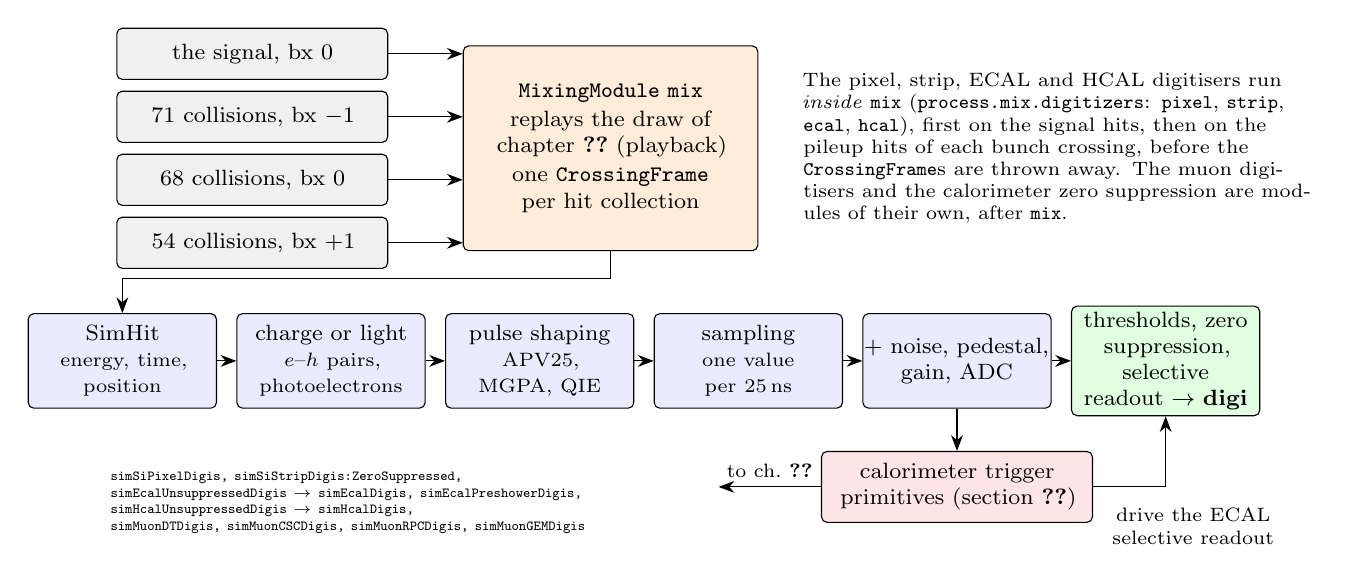
\begin{tikzpicture}[x=1cm, y=1cm, font=\footnotesize, >={Stealth[length=2mm]},
  box/.style={draw, rounded corners=2pt, minimum height=12mm, text width=2.25cm, align=center, inner sep=2pt},
  inp/.style={box, fill=black!6, text width=3.3cm, minimum height=6.5mm},
  mix/.style={box, fill=orange!15, text width=3.6cm, minimum height=26mm},
  st/.style={box, fill=blue!8}, outb/.style={box, fill=green!12}, tp/.style={box, fill=red!10, text width=3.3cm, minimum height=9mm}]
\node[inp] (s)  at (1.65,3.15) {the signal, bx 0};
\node[inp] (m1) at (1.65,2.35) {71 collisions, bx $-1$};
\node[inp] (z)  at (1.65,1.55) {68 collisions, bx 0};
\node[inp] (p1) at (1.65,0.75) {54 collisions, bx $+1$};
\node[mix] (mix) at (6.2,1.95) {\code{MixingModule} \code{mix}\\[1pt] replays the draw of chapter~\ref{ch:10_SIM} (playback)\\[1pt] one \code{CrossingFrame} per hit collection};
\foreach \n in {s,m1,z,p1} \draw[->] (\n.east) -- (mix.west|-\n.east);
\node[text width=6.4cm, align=left, font=\scriptsize] at (11.85,1.95) {The pixel, strip, ECAL and HCAL digitisers run \emph{inside}
\code{mix} (\code{process.mix.digitizers}: \code{pixel}, \code{strip}, \code{ecal}, \code{hcal}), first on the signal hits, then on the
pileup hits of each bunch crossing, before the \code{CrossingFrame}s are thrown away. The muon digitisers and the
calorimeter zero suppression are modules of their own, after \code{mix}.};
\node[st] (c1) at (0.0,-0.75) {SimHit\\{\scriptsize energy, time, position}};
\node[st] (c2) at (2.65,-0.75) {charge or light\\{\scriptsize $e$--$h$ pairs, photo\-electrons}};
\node[st] (c3) at (5.3,-0.75) {pulse shaping\\{\scriptsize APV25, MGPA, QIE}};
\node[st] (c4) at (7.95,-0.75) {sampling\\{\scriptsize one value per 25\,ns}};
\node[st] (c5) at (10.6,-0.75) {$+$ noise, pedestal, gain, ADC};
\node[outb] (c6) at (13.25,-0.75) {thresholds, zero suppression, selective readout $\rightarrow$ \textbf{digi}};
\foreach \a/\b in {c1/c2,c2/c3,c3/c4,c4/c5,c5/c6} \draw[->] (\a) -- (\b);
\draw[->] (mix.south) -- ++(0,-0.35) -| (c1.north);
\node[tp] (tp) at (10.6,-2.35) {calorimeter trigger primitives (section~\ref{sec:11_tp})};
\draw[->] (c5.south) -- (tp.north);
\draw[->] (tp.east) -| (c6.south);
\node[font=\scriptsize, align=center] at (13.6,-2.85) {drive the ECAL\\selective readout};
\draw[->] (tp.west) -- ++(-1.3,0) node[above, pos=0.5, font=\scriptsize] {to ch.~\ref{ch:12_L1T}};
\node[text width=6.6cm, align=left, font=\tiny] at (3.15,-2.55) {\ttfamily simSiPixelDigis, simSiStripDigis:ZeroSuppressed,\\
simEcalUnsuppressedDigis $\rightarrow$ simEcalDigis, simEcalPreshowerDigis,\\
simHcalUnsuppressedDigis $\rightarrow$ simHcalDigis,\\ simMuonDTDigis, simMuonCSCDigis, simMuonRPCDigis, simMuonGEMDigis};
\end{tikzpicture}
\caption{The chain of the \code{DIGI} step. Top: the hits of the signal and of the 193 pileup collisions of chapter~\ref{ch:10_SIM}
are put side by side, each collision shifted in time by $25\ns$ per bunch crossing (bx). Bottom: what every digitiser
does to the hits of one channel, and the modules that write the digis (bottom left). The calorimeters make, from
their unsuppressed frames, a coarse copy for the Level-1 trigger, which in the ECAL also decides which frames are
written.}
\label{fig:11_chain}
\end{figure}

\begin{table}[!htb]
\centering\small\setlength{\tabcolsep}{3.5pt}
\caption{The digitisers at a glance: what the electronics does, and what goes in and comes out for the signal alone
and for the signal with its bunch crossing (\code{ledger\_11\_DIGI.txt}; the HCAL frames from the FWLite extras of the
companion). Each row is one subsection of section~\ref{sec:11_numbers}.}
\label{tab:11_glance}
\begin{tabular}{@{}l>{\raggedright\arraybackslash}p{5.0cm}>{\raggedright\arraybackslash}p{3.0cm}rr@{}}
\toprule
 & what the electronics does & signal: in & signal: out & with pileup: out \\
\midrule
mixing & overlays 193 collisions of bx $-1$, 0, $+1$, times shifted by $\mp25\ns$ & 10\,272 tracker hits & -- & 448\,315 tracker hits \\
pixels & charge above 1600--2000\,$e$ in a $100\times150\,\mu$m$^2$ pixel, an 8-bit ADC, a $\pm12.5\ns$ window & 1902 \code{PSimHit}s & 4800 digis & 77\,980 \\
strips & APV25 pulse in deconvolution mode, zero suppression at 5 (2) times the noise & 8370 \code{PSimHit}s & 31\,602 digis & 436\,901 \\
ECAL, ES & photoelectrons, 10 samples of 25\,ns, selective readout; ES 3 samples & 5521 + 6214 + 1069 cells & 156 + 384 + 981 & 964 + 2520 + 15\,972 \\
HCAL & SiPM or PMT, QIE charge code, 10 (HF: 3) slices, zero suppression & 821 HB/HE, 1 HO, 531 HF cells & 4459 + 0 + 3456 & 6545 + 2 + 3456 \\
muon & drift times, strip samples, bunch crossings & no hit & 8 (RPC noise) & 2016 \\
\midrule
all & & & 44\,172 & 544\,407 \\
\bottomrule
\end{tabular}
\end{table}

The chapter digitises three samples with the same configuration (\path{test/11_DIGI/run_11_DIGI.sh}): (11a) the signal
alone, no mixing; (11b) one library collision alone, library event 72, the first in-time collision of our bunch
crossing; and (11a+11b) the production case, the signal with its 71, 68 and 54 collisions in bunch crossings $-1$, 0
and $+1$. The sample (11b) exists only in this book: in the production the collisions are never digitised one by one.
Run~3 and Phase-2 use \emph{premixing}: a first job mixes and digitises the whole pileup of a bunch crossing into a
library of premixed events (\code{premix\_stage1}), a second job digitises the signal alone and adds one premixed
event to it digi by digi (\code{PreMixingModule}, \path{Configuration/StandardSequences/python/DataMixerPreMix_cff.py}).
The classical mixing of this chapter does the same in one job and keeps every pileup hit in memory, which is what
lets the analyzer tell the origin of every digi.

\emph{How the chapter is organised.} Section~\ref{sec:11_numbers} has one subsection per row of
table~\ref{tab:11_glance}: the mixing and the time windows, then the pixels, the strips, the ECAL, the HCAL and the
muon chambers. Each says, like a step of chapter~\ref{ch:12_L1T}, what the electronics does, which parameters decide
it and where they are set, and what it made of our event, with one data frame or one channel followed by hand. A
subsection then puts the three samples side by side and one says what the 2025 conditions changed. The section
``Made here for the next stage'' explains the calorimeter trigger primitives that this job makes for the Level-1
trigger of chapter~\ref{ch:12_L1T}.

\section{From the previous chapter}

Three files of chapter~\ref{ch:10_SIM} enter (Rule E). The signal, \path{test/10_SIM/out/step2_SIM_signal_10_SIM.root},
is the full Geant4 event: 1926 \code{SimTrack}s from 571 primaries, $10\,272$ tracker \code{PSimHit}s (PXB 929, PXF 973,
TIB 1182, TID 975, TOB 1022, TEC 5191, $2.33\GeV$ of energy loss) and $26\,793$ \code{PCaloHit}s in $14\,157$ cells
(EB 5521 cells with $68.0\GeV$, EE 6214 with $293.7\GeV$, ES 1069, HB 173, HE 648, HO 1, HF 531 cells with 1849
photoelectrons of the shower library), no muon-chamber hit. The library,
\path{step2_SIM_pileup_10_SIM.root}, holds the 250 minimum-bias collisions through the same Geant4; library event 72
has 164 primaries, 2097 tracker hits, 11 CSC hits, 1217 EB cells with $9.4\GeV$, 1948 EE cells with $43.5\GeV$, 223
ES, 21 HB, 101 HE and 119 HF cells. The third file, \path{step3_MIX_10_SIM.root}, is the signal again with one new
product: the \code{CrossingFramePlaybackInfoNew} that the chapter-10 mixing job wrote, the list of which library
events it drew into which bunch crossing. That mixing put $448\,315$ tracker \code{PSimHit}s in front of the
digitisers: $10\,272$ of the signal, $146\,028$ of the 68 in-time collisions, $139\,551$ of the 71 early ones and
$152\,464$ of the 54 late ones.\footnote{Signal hits from \path{test/10_SIM/out/simHits_signal_10_SIM.log}, the
bunch crossing from \path{step3_MIX_10_SIM.log}; library event 72, the zero suppression and the truth counts from
FWLite (companion, section~4); every digi count from \path{test/11_DIGI/out/ledger_11_DIGI.txt}; the data frames
followed by hand and the charges from \path{examples_11_DIGI.txt} (\path{test/11_DIGI/digiExamples_11_DIGI.py}).}

The job runs with the 2025 settings of the release, as chapters~\ref{ch:08_PU}--\ref{ch:10_SIM}; unlike there, the
year changes the result here, because the digitisers read conditions of the global tag that differ in 2025 (the
python thresholds are those of 2024). Section~\ref{sec:11_year} says what changed.

\begin{plainwords}[What a digi is]
A pixel digi is a pixel address and an 8-bit ADC count; a strip digi the same for a strip, kept only if it passed the
zero suppression of the front-end driver; an ECAL digi is a \emph{data frame}, the ten 40-MHz samples of the pulse of
one crystal with the gain of each sample; an HCAL digi is the QIE frame, 10 (HB, HE) or 3 (HF) time slices of the
charge; a DT digi is a wire and a drift time, a CSC digi a strip with 8 samples or a wire group with a time, an RPC
or GEM digi a strip and a bunch crossing. The digitisers are configured in the python of the \code{DIGI} process
(\code{process.mix.digitizers} for the tracker and the calorimeters, the modules \code{simMuon*Digis} for the
chambers); \path{test/11_DIGI/out/thresholds_11_DIGI.txt} lists every threshold, noise and window the job used.
\end{plainwords}

Nothing of the SIM content changes: the \code{DIGI} process copies the generator record, the \code{SimTrack}s and
the signal hits unchanged and adds its products under the process name \code{DIGI}: one digi collection per
subdetector (\code{simSiPixelDigis}, \code{simSiStripDigis}, \code{simEcalDigis}, \code{simHcalDigis},
\code{simMuon*Digis}, \ldots), the \code{DigiSimLink}s, the trigger primitives, the \code{TrackingParticle}s of
\code{mix:MergedTrackTruth} (999 for the signal, $45\,282$ in the mixed event, of which $14\,729$ in-time and
$29\,554$ out-of-time pileup) and the \code{PileupSummaryInfo} with the number of collisions per bunch crossing. The
pileup \code{SimTrack}s and hits themselves are not written; the \code{CrossingFrame}s live only inside the job.

\section{The numbers of the event}
\label{sec:11_numbers}

Table~\ref{tab:11_cuts} is the part of \path{thresholds_11_DIGI.txt} that decides what becomes a digi; the
subsections below take it row by row. Two things are worth seeing at once. First, several thresholds are not numbers
in the configuration but database payloads of the global tag \code{150X\_mcRun3\_2025\_realistic\_v1}: the strip
zero-suppression thresholds, the ECAL selective-readout settings (\code{configFromCondDB = True}), the preshower
threshold and the HCAL zero-suppression levels (\code{useConfigZSvalues = 0}: the \code{HBlevel = 8}, \code{HElevel =
9}, \code{HOlevel = 24} of the python are not used). Second, the time windows differ by an order of magnitude between
subdetectors, and this is what decides how much of the out-of-time pileup survives.

\begin{table}[htb]
\centering\footnotesize\setlength{\tabcolsep}{4pt}
\caption{The cuts of the digitisers of the mixed configuration (\code{test/11\_DIGI/out/thresholds\_11\_DIGI.txt}, the
parameter sets of \code{process.mix.digitizers} and of the modules after the mixing; the payloads from \code{conddb
dump}, companion section~4). ``DB'' means the value is a payload of the global tag, not a number in the python.}
\label{tab:11_cuts}
\begin{tabular}{p{1.4cm}p{14.2cm}}
\toprule
digitiser & what decides whether a channel becomes a digi \\
\midrule
pixel & charge above \code{ThresholdInElectrons} $=1600$\,e (BPix layer 1: 2000\,e), smeared by 245\,e (BPix) / 210\,e
(FPix); noise 175\,e per pixel plus 350\,e readout noise, noisy pixels added; ADC from a fixed non-linear response
(\code{BPix\_SignalResponse\_p0..p3}), 8 bits; time window \code{TofLowerCut/TofUpperCut} $=-12.5/+12.5\ns$; Lorentz
angle, dead modules and bad FED channels from DB; inefficiency on \\
strip & APV in deconvolution mode, hits within \code{TOFCutForDeconvolution} $=50\ns$, weighted by the APV pulse
(\path{APVShapeDeco_320.txt}); per-strip pedestals and noise from DB, common-mode noise RMS 5.92 / 3.08 / 1.08 / 2.44
ADC (TIB / TID / TOB / TEC); 247\,e per ADC count; FED zero suppression \code{FedAlgorithm = 4}: a strip above 5 times
its noise, or above 2 times with a neighbour above 2 times (DB, \code{SiStripThreshold\_Ideal\_31X\_v2}) \\
ECAL & 2250 (EB) / 1800 (EE) photoelectrons per GeV, laser correction from DB, pulse shape from DB, 10 samples, peak
in sample 6, correlated noise (the \code{CorrNoiseMatrix} vectors), constant term 0.3\,\%; selective readout
(\code{simEcalDigis}) from DB, driven by the trigger primitives: full readout of the trigger towers / supercrystals
flagged high interest, zero suppression elsewhere ($0.3325\GeV$ EB, $0.36\GeV$ EE); ES: 3 samples, threshold of 6 ADC
counts on sample 2 (DB, \code{ESThresholds\_LG\_V03\_mc}) \\
HCAL & HB / HE: photoelectrons per GeV from the sampling factors 125 (HB) and 186--211 (HE) and the gain and SiPM
parameters of DB, SiPM and time smearing, 10 time slices with the sample of interest at 6, TDC threshold 18.7; HF:
6 photoelectrons per shower-library unit, sampling factor 0.37, 3 time slices; zero suppression (\code{simHcalDigis})
on the sample of interest (\code{use1ts}) with levels from DB, none for HF; a frame for every channel
(\code{doEmpty = True}) \\
muon & DT: drift time smeared by 2.4\,ns, dead time 150\,ns, links within 10\,ns; CSC: strip pedestals, gains and noise
from DB (\code{stripConditions = Database}), 8 SCA samples of 50\,ns, strips integrated from $-250$ to $+500\ns$,
read in boards of 16 strips; RPC: efficiency 0.95, gate 25\,ns, noise and background on; GEM: efficiency 0.98,
intrinsic noise off, window bx $-5$ to $+3$ \\
\bottomrule
\end{tabular}
\end{table}

\subsection{The mixing, and the time windows of the digitisers}
\label{sec:11_mix}

\textbf{What it does.} The \code{MixingModule} reads, for every bunch crossing of its window, the requested number of
library collisions and gives each of their hits two labels: the bunch crossing and the number of the collision in it,
packed into an \code{EncodedEventId}. It also shifts the time of every hit by $25\ns$ per bunch crossing
(\path{SimGeneral/MixingModule/plugins/Adjuster.cc}: \code{timeOffset = bcr * bunchSpace}): a hit of
bunch crossing $-1$ arrives $25\ns$ before ours, one of $+1$ $25\ns$ after. The hits of all collisions and of the
signal are then put in one \code{CrossingFrame} per collection, and the digitisers inside the module run on it. Nothing
in the digitisers knows about collisions: they see charges arriving at times, and the time is what will separate the
crossings, or fail to.

\textbf{The parameters.} \code{AVE\_60\_BX\_25ns} with \code{N = 60}, \code{B = (-1, 1)}: a Poisson draw of mean 60
collisions in each of three crossings $25\ns$ apart, the library read in sequence (\code{input.sequential = True}) and,
for this book, \code{playback = True} (box below).

\begin{plainwords}[Why the DIGI job replays the chapter-10 draw]
The \code{MixingModule} draws the number of collisions per bunch crossing from a Poisson distribution of mean 60
(seed 12345 of the module \code{mix}) and reads the library in sequence. Chapter~\ref{ch:10_SIM}
drew 71, 68 and 54. The same module with the same seed in this chapter would \emph{not}: in
\code{BMixingModule::produce} (\path{Mixing/Base/src/BMixingModule.cc}) the order is \code{initializeEvent},
\code{addSignals}, then \code{doPileUp}, and \code{addSignals} runs the digitisers on the signal, which consume random
numbers from the same engine (noise, photostatistics, threshold smearing) before \code{PileUp::CalculatePileup}
(\path{Mixing/Base/src/PileUp.cc}, called from \path{SimGeneral/MixingModule/plugins/MixingModule.cc}) draws the
number of collisions. In chapter~\ref{ch:10_SIM} no digitiser ran, so the draw came first; here a fresh draw gave
65, 67 and 56 when it was tried. The script therefore sets \code{process.mix.playback = True}: the module reads the
\code{CrossingFramePlaybackInfoNew} of \path{step3_MIX_10_SIM.root} and mixes exactly library events 1--71, 72--139
and 140--193; the \code{PileupSummaryInfo} then reports 71, 68 and 54 as the ``true'' number of interactions, not 60.
\end{plainwords}

\textbf{The time windows.} Each digitiser looks at a different stretch of time around our crossing, and
figure~\ref{fig:11_windows} draws them on one axis. The pixels accept a hit only if it arrives within $\pm12.5\ns$ of
the time a particle travelling at the speed of light from the centre of the detector would need
(\code{TofLowerCut/TofUpperCut}): one crossing, nothing else. The strips accept $\pm50\ns$, but weight the charge with
the APV pulse, which is non-zero only from $28\ns$ before to $30\ns$ after its peak. The calorimeters write ten
samples of $25\ns$, from five samples before the in-time peak to four after it, and their pulses last longer than
that. The muon chambers are slower still: a DT wire sees electrons drift for hundreds of nanoseconds, a CSC strip
integrates from $-250$ to $+500\ns$. The mixing of this book offers three crossings; the production profile of 2025
mixes from $-12$ to $+3$ (chapter~\ref{ch:10_SIM}), because the slow detectors remember that far back.

\begin{figure}[!htb]
\centering
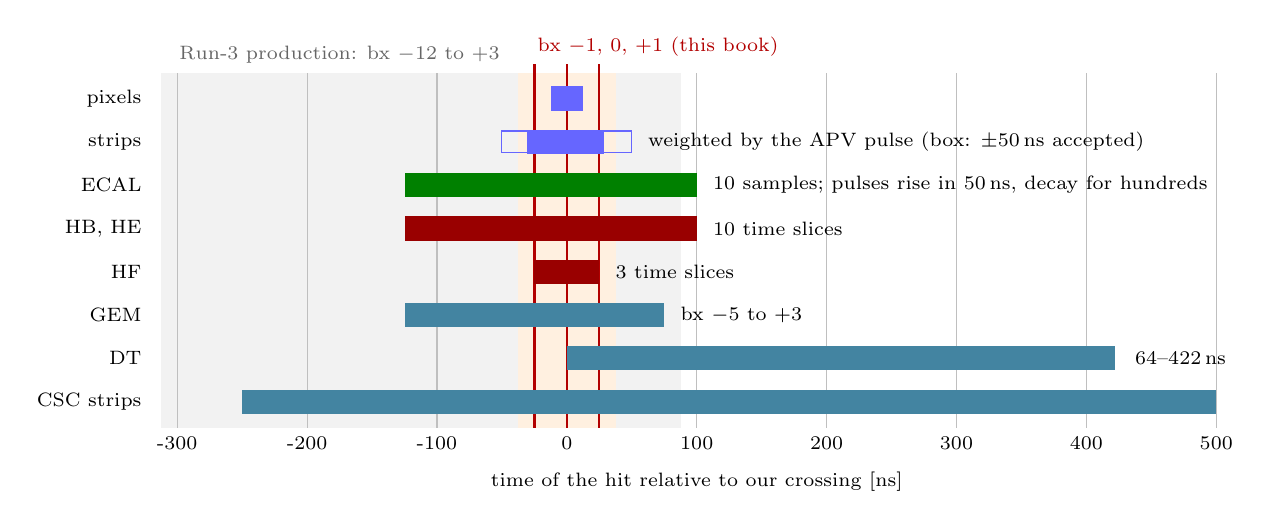
\begin{tikzpicture}[x=0.0165cm, y=0.55cm, font=\scriptsize]
\fill[orange!12] (-37.5,0.4) rectangle (37.5,8.6);
\fill[black!5] (-312.5,0.4) rectangle (-37.5,8.6); \fill[black!5] (37.5,0.4) rectangle (87.5,8.6);
\foreach \t in {-300,-200,-100,0,100,200,300,400,500} { \draw[black!25] (\t,0.4) -- (\t,8.6); \node[below] at (\t,0.4) {\t}; }
\foreach \t in {-25,0,25} \draw[red!70!black, thick] (\t,0.4) -- (\t,8.8);
\node[above right, red!70!black] at (-30,8.75) {bx $-1$, 0, $+1$ (this book)};
\node[black!60, above] at (-175,8.6) {Run-3 production: bx $-12$ to $+3$};
\node[below] at (100,-0.4) {time of the hit relative to our crossing [ns]};
\foreach \y/\lab/\a/\b/\c in {8/pixels/-12.5/12.5/blue!60, 7/strips/-30.5/28.4/blue!60,
  6/ECAL/-125/100/green!50!black, 5/{HB, HE}/-125/100/red!60!black, 4/HF/-25/25/red!60!black,
  3/GEM/-125/75/cyan!60!black, 2/DT/0/422/cyan!60!black, 1/CSC strips/-250/500/cyan!60!black}
  { \node[left] at (-320,\y) {\lab}; \fill[\c] (\a,\y-0.28) rectangle (\b,\y+0.28); }
\draw[blue!60] (-50,6.75) rectangle (50,7.25);
\node[right] at (55,7) {weighted by the APV pulse (box: $\pm50\ns$ accepted)};
\node[right] at (105,6) {10 samples; pulses rise in $50\ns$, decay for hundreds};
\node[right] at (105,5) {10 time slices};
\node[right] at (30,4) {3 time slices};
\node[right] at (80,3) {bx $-5$ to $+3$};
\node[right] at (430,2) {64--422\,ns};
\end{tikzpicture}
\caption{The time windows of the digitisers (schematic; the limits are the parameters of \code{thresholds\_11\_DIGI.txt}
and of the muon \code{cfi} files, the pulse limits those of figures~\ref{fig:11_si} and~\ref{fig:11_frames}). Red lines:
the three bunch crossings mixed in this book (orange band); grey: the out-of-time window of the 2025 production
profile, $-12$ to $+3$. The DT bar spans the 12 DT digis of the event, 64 to $422\ns$ after the fixed offset of the
synchronisation.}
\label{fig:11_windows}
\end{figure}

\textbf{The numbers of the event.} The \code{CrossingFrame}s hold $448\,315$ tracker hits: $10\,272$ of the signal,
$146\,028$ in time, $139\,551$ early and $152\,464$ late. Two thirds of what the tracker digitisers receive is out of
time, and the windows decide what becomes of it: the pixels make $77\,980$ digis of their $87\,653$ hits (0.9 per hit,
against 2.5 for the signal alone), the strips $436\,901$ of their $360\,662$ (1.2 per hit). The truth survives the
mixing: $45\,282$ \code{TrackingParticle}s, 999 of the signal, $14\,729$ of the in-time and $29\,554$ of the
out-of-time collisions.

\FloatBarrier
\subsection{The pixels}
\label{sec:11_pixel}

\textbf{What it does.} A pixel module is a sensor of silicon, 285\,$\mu$m thick in the simulated geometry
(\path{Geometry/TrackerCommonData/data/PhaseI/pixbarladder.xml}, \code{SensorThick}), divided into pixels of
$100\times150\,\mu$m$^2$ and bump-bonded to readout chips (ROCs) of $80\times52$ pixels
(\path{trackerStructureTopology.xml}). A charged particle frees one electron--hole pair per $3.61$\,eV it loses
(\code{GeVperElectron} of the pixel digitiser, \path{SiPixelDigitizerAlgorithm.cc}). The digitiser cuts
the path of the \code{PSimHit} into segments, draws the energy loss of each with Landau fluctuations, and drifts the
electrons to the readout side of the sensor. On the way two things spread them: diffusion ($3.7\,\mu$m per
$300\,\mu$m of drift, \code{Sigma0}), and the magnetic field. In the $3.8$\,T field the electrons do not drift straight
along the electric field but at the \emph{Lorentz angle} to it, so that the charge made at the far side of the sensor
lands tens of micrometres sideways. The charge collected by each pixel is compared with a threshold, and a pixel above it
becomes a digi with an 8-bit ADC count.

\textbf{The parameters.} The threshold is 1600 electrons (2000 in the first barrel layer), smeared from pixel to pixel
by 245 (210 in the disks); the noise is 175 electrons per pixel. The ADC is not a straight line: the digitiser
converts the charge to the calibration unit of the chip (\code{ElectronsPerVcal = 47}, 50 in layer~1) and applies the
response $148+203\tanh(0.00171\,v-0.711)$ of the \code{SignalResponse} parameters, which saturates at 255
(figure~\ref{fig:11_si}, left). The Lorentz angle comes from the payload
\code{SiPixelLorentzAngleSim\_phase1\_EoR3\_HV800\_Tr2000}: $\tan\theta_L$ per tesla 0.0358 in layer~1, 0.0709 in
layers 3 and 4.

\begin{plainwords}[A worked example: one particle through one pixel module]
The signal has 592 barrel-pixel hits that cross the full 285\,$\mu$m. Their charge per micrometre of path has a median
of 84 electrons (\code{examples\_11\_DIGI.txt}), so a particle crossing at right angles frees about $84\times285=
24\,000$ electrons: \emph{fifteen times} the threshold of 1600, \emph{140 times} the noise of a pixel. That margin is
why the pixels are clean: not one of the 4800 pixel digis of the signal is noise. In layer~1 the Lorentz angle moves the
charge of the far side by $0.0358\times3.8\times285 = 39\,\mu$m, two fifths of a pixel, in layers 3 and 4 by
$77\,\mu$m: the charge is shared by neighbouring pixels, and the reconstruction will use the sharing to measure the
position better than the pitch. Shared among 2.5 pixels, $24\,000$ electrons give some 9600 per pixel, ADC 78 on the
curve; the median pixel digi of the signal has ADC 69.
\end{plainwords}

\textbf{The numbers of the event.} The 1902 pixel hits of the signal become 4800 digis, 2.5 per hit, all linked to a
signal particle (PXB 3011, PXF 1789). Their ADC counts have a median of 69 (a quarter below 46, a quarter above 105),
and 170 are at full scale, 255: the response saturates at $35\,600$ electrons, which a slow or grazing particle exceeds
in one pixel. In the bunch crossing the pixels make $77\,980$ digis: 4603 of the signal, $71\,575$ in time, 1802 early,
none late, none without a link. The window explains the last three numbers. A hit of bunch crossing $+1$ arrives at
least $25\ns$ late and is always outside $\pm12.5\ns$. A hit of bunch crossing $-1$ arrives $25\ns$ early and gets in
only if its own flight took $12.5$ to $37.5\ns$ longer than light would: a looper, a slow proton, a secondary made late
in a shower. 1802 such hits are not few; the asymmetry is that a particle can be late but never early.

\begin{figure}[!htb]
\centering
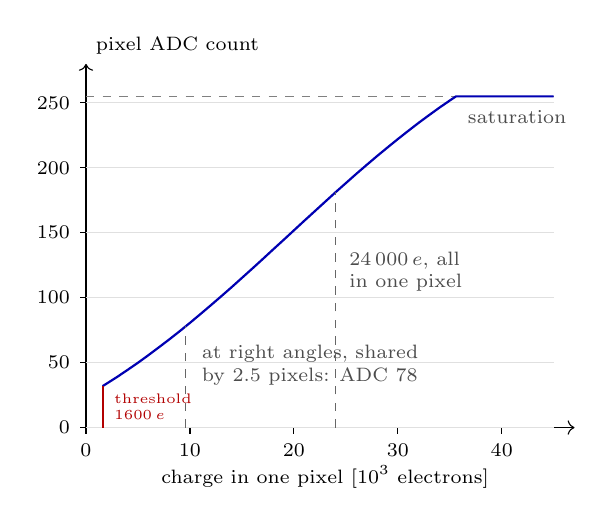
\begin{tikzpicture}[x=0.132cm, y=0.0165cm, font=\scriptsize]
\draw[->] (0,0) -- (47,0);
\node[below] at (23,-22) {charge in one pixel [$10^3$ electrons]};
\draw[->] (0,0) -- (0,280) node[above right] {pixel ADC count};
\foreach \x in {0,10,20,30,40} \draw (\x,0) -- (\x,-5) node[below] {\x};
\foreach \y in {0,50,100,150,200,250} { \draw (0,\y) -- (-0.6,\y) node[left] {\y}; \draw[black!12] (0,\y) -- (45,\y); }
\draw[black!50, dashed] (0,255) -- (45,255);
\draw[blue!70!black, thick] plot coordinates {(1.6,31.9) (2.0,33.9) (3.0,39.0) (4.0,44.4) (5.0,49.9) (6.0,55.7) (7.0,61.7) (8.0,67.8) (9.0,74.1) (10.0,80.6) (11.0,87.3) (12.0,94.1) (13.0,101.0) (14.0,108.0) (15.0,115.2) (16.0,122.4) (17.0,129.7) (18.0,137.1) (19.0,144.4) (20.0,151.8) (21.0,159.2) (22.0,166.5) (23.0,173.8) (24.0,181.1) (25.0,188.2) (26.0,195.3) (27.0,202.2) (28.0,209.0) (29.0,215.6) (30.0,222.1) (31.0,228.4) (32.0,234.6) (33.0,240.5) (34.0,246.3) (35.0,251.8) (35.6,255.0) (45.0,255.0)};
\draw[red!70!black, thick] (1.6,0) -- (1.6,31.9);
\node[red!70!black, right, align=left, font=\tiny] at (1.8,16) {threshold\\$1600\,e$};
\draw[black!60, dashed] (9.6,0) -- (9.6,78);
\node[black!70, right, align=left] at (10.2,48) {at right angles, shared\\by 2.5 pixels: ADC 78};
\draw[black!60, dashed] (24,0) -- (24,181.1);
\node[black!70, right, align=left] at (24.4,120) {$24\,000\,e$, all\\in one pixel};
\node[black!70, below right] at (35.8,252) {saturation};
\end{tikzpicture}\hfill
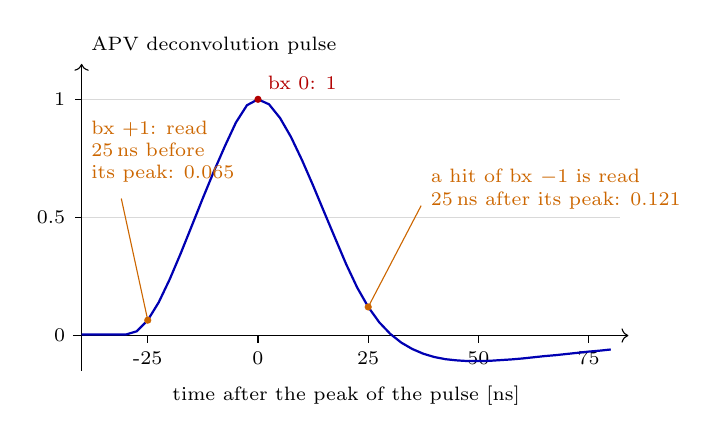
\begin{tikzpicture}[x=0.056cm, y=3.0cm, font=\scriptsize]
\draw[->] (-42,0) -- (84,0);
\node[below] at (20,-0.17) {time after the peak of the pulse [ns]};
\draw[->] (-40,-0.15) -- (-40,1.15) node[above right] {APV deconvolution pulse};
\foreach \x in {-25,0,25,50,75} \draw (\x,0) -- (\x,-0.03) node[below] {\x};
\foreach \y in {0,0.5,1} \draw (-40,\y) -- (-41.5,\y) node[left] {\y};
\draw[black!15] (-40,0.5) -- (82,0.5); \draw[black!15] (-40,1) -- (82,1);
\draw[blue!70!black, thick] plot coordinates {(-40.0,0.004) (-37.5,0.004) (-35.0,0.004) (-32.5,0.004) (-30.0,0.004) (-27.5,0.018) (-25.0,0.065) (-22.5,0.141) (-20.0,0.239) (-17.5,0.349) (-15.0,0.465) (-12.5,0.582) (-10.0,0.695) (-7.5,0.802) (-5.0,0.902) (-2.5,0.975) (0.0,1.000) (2.5,0.979) (5.0,0.921) (7.5,0.840) (10.0,0.742) (12.5,0.635) (15.0,0.523) (17.5,0.412) (20.0,0.302) (22.5,0.203) (25.0,0.121) (27.5,0.056) (30.0,0.007) (32.5,-0.030) (35.0,-0.057) (37.5,-0.077) (40.0,-0.091) (42.5,-0.100) (45.0,-0.105) (47.5,-0.108) (50.0,-0.108) (52.5,-0.107) (55.0,-0.104) (57.5,-0.101) (60.0,-0.097) (62.5,-0.092) (65.0,-0.087) (67.5,-0.083) (70.0,-0.078) (72.5,-0.073) (75.0,-0.068) (77.5,-0.064) (80.0,-0.059)};
\fill[red!70!black] (0,1) circle (1.3pt) node[above right] {bx 0: 1};
\fill[orange!80!black] (25,0.121) circle (1.3pt);
\draw[orange!80!black] (25,0.121) -- (37,0.55);
\node[orange!80!black, right, align=left] at (37,0.62) {a hit of bx $-1$ is read\\$25\ns$ after its peak: 0.121};
\fill[orange!80!black] (-25,0.065) circle (1.3pt);
\draw[orange!80!black] (-25,0.065) -- (-31,0.58);
\node[orange!80!black, right, align=left] at (-40,0.78) {bx $+1$: read\\$25\ns$ before\\its peak: 0.065};
\end{tikzpicture}
\caption{The response of the silicon readout, from the release. Left: the ADC count of a pixel as a function of its
charge, the response of \code{SiPixelDigitizerAlgorithm::missCalibrate} with the parameters of
\code{thresholds\_11\_DIGI.txt} (BPix layers 2--4 and FPix); the marks use the median charge of the signal hits,
84 electrons per $\mu$m. Right: the APV25 pulse in deconvolution mode, \code{SimTracker/SiStripDigitizer/data/APVShapeDeco\_320.txt},
by which the strip digitiser multiplies the charge of a hit according to its arrival time
(\code{SiLinearChargeDivider::TimeResponse}).}
\label{fig:11_si}
\end{figure}

\subsection{The strips}
\label{sec:11_strip}

\textbf{What it does.} The strip tracker uses the same silicon, cut into long strips some 80 to 200\,$\mu$m apart; in the
simulated geometry the sensors of the TIB and TID are 290\,$\mu$m thick, those of the TOB and of the outer TEC rings
470\,$\mu$m (the largest distance between the entry and exit points of the signal hits). Each strip is read by one
channel of an APV25 chip. The chip amplifies the charge into a pulse about $50\ns$ long and stores samples of it every
$25\ns$; in \emph{deconvolution mode}, the mode of collisions, it adds three consecutive samples with weights that undo
most of the pulse length, so that what is read for a crossing is a pulse only $25$--$30\ns$ wide on each side of its
peak (figure~\ref{fig:11_si}, right). The digitiser takes the charge of a hit, shares it among the strips it crosses,
leaks a fraction to the neighbours (cross-talk: in the inner barrel 84\,\% stays in the strip, 7\,\% goes to each
neighbour, \code{CouplingConstantRunIIDecIB1}), multiplies it by the pulse at the arrival time, and converts it at
247 electrons per ADC count. It then adds the pedestal and noise of every strip and a common-mode noise shared by the
128 strips of a chip, and applies the zero suppression of the front-end driver (FED).

\textbf{The parameters.} The FED algorithm 4 keeps a strip whose charge is above 5 times its noise, or above 2 times if
a neighbour is too (and a few rarer patterns of neighbours); the factors 5 and 2 are the payload
\code{SiStripThreshold\_Ideal\_31X\_v2}, the noise of each strip is \code{SiStripNoises}. The common-mode RMS is 5.92,
3.08, 1.08 and 2.44 ADC counts in the TIB, TID, TOB and TEC.

\begin{plainwords}[A worked example: why the strips have noise digis and the pixels none]
A particle crossing a TIB sensor at right angles frees $93.5\times290\approx27\,000$ electrons, 110 ADC counts at 247
electrons per count, shared by three strips on average: the signal digis have a median of 64 counts. The thresholds
sit at only 5 and 2 times the noise of a strip, because the strips are long and their noise large. A Gaussian
fluctuation passes 2 times the noise in 2.3\,\% of the strips; that two neighbours do so together happens about once
per thousand strips, and the strip tracker has some ten million. Hence the $12\,184$ strips without a link in the
signal sample, with a median of 18 counts and none above 85: noise that passed the zero suppression, the same in every
event whatever the collision ($12\,234$ for library event 72). The pixels, with a threshold at nine times their noise,
have none.
\end{plainwords}

\textbf{The numbers of the event.} The 8370 strip hits of the signal become $19\,418$ linked digis, 2.3 per hit, in
6473 clusters of 3.0 adjacent strips; 990 of them are at the top of the 8-bit range. In the bunch crossing the strips
make $436\,901$ digis: $19\,162$ of the signal, $279\,143$ in time, $121\,942$ early (28\,\%), 7029 late and 9625 with
no link. Why so many early ones and so few late? Figure~\ref{fig:11_si} answers half of it: a hit of bunch crossing $-1$
is read $25\ns$ after the peak of its pulse, where the pulse is still at 12\,\% of its height; one of $+1$ is read
$25\ns$ before its peak, at 6.5\,\%. The other half is the asymmetry of the pixels: a particle arrives later than light,
never earlier, so any delay moves an early hit up the falling edge (at $+20\ns$ the pulse is at 30\,\%) and a late hit
down the rising one (at $-30\ns$ it is at 0.4\,\%). Near a threshold of a few times the noise, these factors decide
whether a strip is written.

\FloatBarrier
\subsection{The ECAL and the preshower}
\label{sec:11_ecal}

\textbf{What it does.} An ECAL crystal of lead tungstate turns the energy of a shower into scintillation light, read
by avalanche photodiodes (APDs) in the barrel and vacuum phototriodes (VPTs) in the endcaps. The digitiser converts
the energy of the hits of a crystal into photoelectrons, 2250 per GeV in the barrel and 1800 in the endcaps, with
Poisson fluctuations (\code{doPhotostatistics}: $\sqrt{2250}=47$, a 2\,\% spread for a GeV), and divides them by the
\emph{laser correction} of the crystal, the fraction of light that the radiation-damaged crystal still transmits
(\code{UseLCcorrection = True}, payload \code{EcalLaserAPDPNRatios}). The light becomes a pulse of the shape stored in
the payload \code{EcalSimPulseShapePhaseI}: it rises in $50\ns$ and decays slowly, to 0.88 of its height one sample
after the peak and 0.32 four samples after it (figure~\ref{fig:11_frames}). The front-end (the MGPA amplifier and a
12-bit ADC) samples it ten times, $25\ns$ apart, with the peak of an in-time pulse in sample~6, at the highest of three
gains (12, 6, 1) that does not saturate, on a pedestal of about 200 counts with noise correlated from sample to sample.
The digitiser puts the full scale of gain 1 at $1668\GeV$ in the barrel and $2860\GeV$ in the endcaps
(\path{SimCalorimetry/EcalSimAlgos/src/EcalCoder.cc}: ``4095(MAXADC)*12(gain 2)*0.035(GeVtoADC)*0.97''), so that at
gain 12 one count is about $34\MeV$ in the barrel and $58\MeV$ in the endcaps, before the intercalibration of the
crystal, and a barrel crystal stays at gain 12 up to some $130\GeV$.

Then comes the decision that makes the ECAL different from every other subdetector: which of the $75\,848$ frames to
write. The \emph{selective readout} (\code{simEcalDigis}) reads in full the trigger towers (barrel) and supercrystals
(endcaps) that the trigger primitives flag as interesting, and applies elsewhere a zero suppression of $0.3325\GeV$ in
the barrel and $0.36\GeV$ in the endcaps to a weighted sum of the samples. Its input is the trigger primitive of every
tower, made in the same job from the unsuppressed frames; section~\ref{sec:11_tp} explains them. The preshower (ES), two
planes of silicon strips in front of the endcaps, keeps 3 samples and writes a strip whose second sample is 6 counts
above the pedestal (\code{ESThresholds\_LG\_V03\_mc}).

\begin{plainwords}[A worked example: one crystal of the $b$ jet]
The barrel crystal $(i\eta,i\phi)=(-82,239)$, at the edge of the barrel next to the $b$ jet, received $3.72\GeV$ in time.
Its frame, the largest of the signal: \code{204 201 200 200 250 265 253 241 231 219}, all at gain 12. The first three
samples are the pedestal, 201.7 on average; the pulse starts in sample 5 and peaks in sample 6, 63 counts above the
pedestal, and the samples that follow fall as the stored shape does (figure~\ref{fig:11_frames}). At $0.035\times0.97$
GeV per count a perfect crystal would give $3.72/0.034=110$ counts; this one gives 63, 17 counts per GeV. Over the 13
barrel crystals with more than $0.5\GeV$ and a frame the median is 18.4 counts per GeV instead of 29.5: the digitiser
divides the light of each crystal by its laser correction (the transparency it has lost to radiation, in the 2025
conditions) and by its intercalibration constant, and these crystals give about 0.6 of the counts of a perfect one.
The same loss weakens the trigger primitives of section~\ref{sec:11_tp}.
\end{plainwords}

\textbf{The numbers of the event.} The signal touched 5521 barrel crystals (5218 of them in time, with $67.1\GeV$),
and 156 frames are written: 100 because 4 trigger towers of 25 crystals are read in full, 56 because they passed the
zero suppression. The threshold is felt: of the crystals with more than $1\GeV$ all 6 are written, of those above
$0.3325\GeV$ 19 of 30, of those above $0.1\GeV$ 24 of 113, and 70 frames have no deposit behind them (the full-readout
towers and noise). In the endcaps, 6214 crystals with $293.7\GeV$ give 384 frames, 355 of them in the 16 supercrystals
read in full. Of the 34 endcap crystals above $1\GeV$, 19 are written, and the line between the two groups is a line in
$\eta$: the 19 are the $b$ jet, at $\abseta=1.55$--1.66; the 15 others, with up to $5.8\GeV$ each, sit at
$\abseta=2.2$--2.9, where the radiation has darkened the crystals most (the laser-monitoring ratio of the 2025
payload is 0.22 at $2<\abseta<2.5$ and 0.013 at $2.5<\abseta<3$, companion section~4.9), and a deposit of several GeV
stays under the zero suppression. Most of the $68\GeV$ the signal left in the barrel is spread over
thousands of crystals with a few MeV each, and is never read out either. In the bunch crossing the barrel writes
964 frames, the endcaps 2520 and the preshower $15\,972$ of its $137\,216$ strips (981 for the signal alone).

\begin{figure}[!htb]
\centering
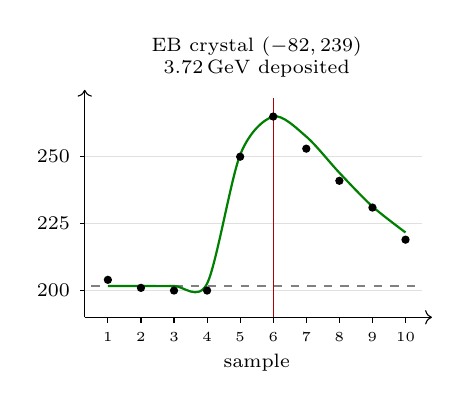
\begin{tikzpicture}[x=0.42cm, y=0.034cm, font=\scriptsize]
\node[above, align=center] at (5.5,276) {EB crystal $(-82,239)$\\$3.72\GeV$ deposited};
\draw[->] (0.3,190) -- (10.8,190);
\node[below] at (5.5,180) {sample};
\draw[->] (0.3,190) -- (0.3,275);
\foreach \x in {1,...,10} \draw (\x,190) -- (\x,188) node[below, font=\tiny] {\x};
\foreach \y in {200,225,250} { \draw (0.3,\y) -- (0.15,\y) node[left] {\y}; \draw[black!12] (0.3,\y) -- (10.5,\y); }
\draw[black!50, dashed] (0.5,201.7) -- (10.5,201.7);
\draw[red!70!black] (6,190) -- (6,272);
\draw[green!50!black, thick] plot[smooth] coordinates {(1,201.7) (2,201.7) (3,201.7) (4,202.6) (5,250.7) (6,265.0) (7,257.5) (8,244.0) (9,231.4) (10,221.7)};
\foreach \x/\y in {1/204,2/201,3/200,4/200,5/250,6/265,7/253,8/241,9/231,10/219} \fill[black] (\x,\y) circle (1.5pt);
\end{tikzpicture}\hfill
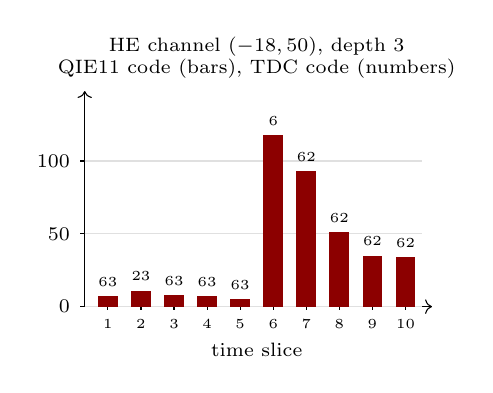
\begin{tikzpicture}[x=0.42cm, y=0.0185cm, font=\scriptsize]
\node[above, align=center] at (5.5,150) {HE channel $(-18,50)$, depth 3\\QIE11 code (bars), TDC code (numbers)};
\draw[->] (0.3,0) -- (10.8,0);
\node[below] at (5.5,-18) {time slice};
\draw[->] (0.3,0) -- (0.3,148);
\foreach \x in {1,...,10} \draw (\x,0) -- (\x,-2) node[below, font=\tiny] {\x};
\foreach \y in {0,50,100} { \draw (0.3,\y) -- (0.15,\y) node[left] {\y}; \draw[black!12] (0.3,\y) -- (10.5,\y); }
\foreach \x/\y/\t in {1/7/63,2/11/23,3/8/63,4/7/63,5/5/63,6/118/6,7/93/62,8/51/62,9/35/62,10/34/62} { \fill[red!55!black] (\x-0.3,0) rectangle (\x+0.3,\y); \node[above, font=\tiny] at (\x,\y) {\t}; }
\end{tikzpicture}\hfill
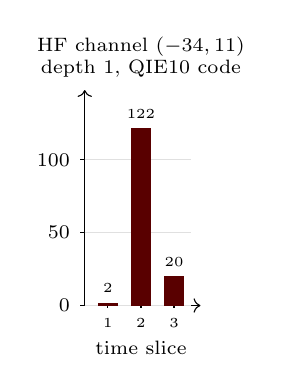
\begin{tikzpicture}[x=0.42cm, y=0.0185cm, font=\scriptsize]
\node[above, align=center] at (2,150) {HF channel $(-34,11)$\\depth 1, QIE10 code};
\draw[->] (0.3,0) -- (3.8,0);
\node[below] at (2,-18) {time slice};
\draw[->] (0.3,0) -- (0.3,148);
\foreach \x in {1,2,3} \draw (\x,0) -- (\x,-2) node[below, font=\tiny] {\x};
\foreach \y in {0,50,100} { \draw (0.3,\y) -- (0.15,\y) node[left] {\y}; \draw[black!12] (0.3,\y) -- (3.5,\y); }
\foreach \x/\y in {1/2,2/122,3/20} { \fill[red!35!black] (\x-0.3,0) rectangle (\x+0.3,\y); \node[above, font=\tiny] at (\x,\y) {\y}; }
\end{tikzpicture}
\caption{Three data frames of the signal, the largest of their kind (\code{examples\_11\_DIGI.txt}). Left: the barrel
crystal of the worked example, its ten samples (dots), the pedestal (dashed), the sample of the in-time peak (red) and
the pulse shape of the payload \code{EcalSimPulseShapePhaseI} scaled to the peak (line). Middle: the HE channel of the $b$-jet tower $(i\eta,i\phi)=
(-18,50)$, its ten QIE11 codes and, above each slice, the TDC code (63: the pulse never crossed the TDC threshold in
that slice; 62: it was already above it when the slice began; 6: it crossed $3\ns$ into the slice). Right: the HF channel of
the $\bar b$-jet tower, three slices.}
\label{fig:11_frames}
\end{figure}

\subsection{The HCAL}
\label{sec:11_hcal}

\textbf{What it does.} The barrel and endcap hadron calorimeters (HB, HE) are brass with plastic scintillator tiles;
the light of each tile is carried by fibres to a silicon photomultiplier (SiPM), and the tiles of a tower are summed
in a few \emph{depths}. The forward calorimeter (HF) is steel with quartz fibres, in which the shower makes Cherenkov
light, read by photomultipliers. The digitiser converts the visible energy of a cell into photoelectrons (for HB and HE
through the sampling factor, 125 in HB and 186 to 211 in HE, which scales the energy seen by the scintillator up to the
energy of the shower, and through the gain and the photoelectrons per femtocoulomb of the SiPM of the database; for
the HF, 6 photoelectrons per unit of the shower library of chapter~\ref{ch:10_SIM}), adds the dark current of the SiPM,
shapes the pulse and integrates it every $25\ns$ in a QIE chip (``charge integrator and encoder''). The QIE writes an
8-bit code that is not linear in the charge: two bits choose one of four ranges, six bits the step inside it, so that
the step grows with the charge. The QIE11 of HB and HE also has a TDC, which says when in the $25\ns$ the pulse crossed a
threshold, in steps of half a nanosecond (\path{SimCalorimetry/HcalSimAlgos/interface/HcalTDCParameters.h}).

\textbf{The parameters.} HB and HE write 10 time slices, with the \emph{sample of interest}, the slice of our
crossing, at 6; the HF writes 3, sample of interest 2; HO 10. The digitiser makes a frame for every channel, hit or not
(\code{doEmpty = True}), so that the noise is everywhere. The zero suppression (\code{HcalRealisticZS}) then keeps a
frame if the code of its sample of interest reaches the level of the channel in the payload
\code{HcalZSThresholds\_2025\_MOY\_mc}: 25.4 on average in HB, 9.0 in HE, 24 in HO; the HF has none.

\textbf{The numbers of the event.} The frames of figure~\ref{fig:11_frames} show what the QIE sees. The HE channel at
the heart of the $b$ jet reads codes 5 to 11 in the first five slices (pedestal and noise; the TDC answers 63, no
crossing, except for a blip at $11.5\ns$ in slice 2), jumps to 118 in slice 6 with the TDC at 6 ($3\ns$ into the slice),
and decays over the next four slices (TDC 62: still above threshold when each began). The HF channel of the
$\bar b$ jet is one slice, 122, between 2 and 20: Cherenkov light is fast. A typical kept frame is much smaller: the
median of the signal sample by its range, HE $(i\eta,i\phi)=(-16,31)$, depth 4, reads \code{4 4 5 7 6 15 12 12 15 12},
a noise fluctuation that passed the level of its channel in slice 6.

Of the $15\,840$ HB and HE frames the zero suppression keeps 4459 for the signal. The signal has hits in only 821 HB and
HE cells, so at least 3600 of the kept frames are noise; library event 72, with hits in 122 cells, keeps 4310. The
HF writes all its 3456 frames in every sample (the analyzer counts the 2270 of the signal with a positive amplitude),
and the HO none (one cell with $4\times10^{-6}\GeV$). In the bunch crossing the zero suppression keeps 6545 HB/HE frames,
2 HO frames, and the summed amplitudes grow from the signal alone by a factor 1.7 in the HB, 7.0 in the HE and 3.7 in
the HF.

\FloatBarrier
\subsection{The muon chambers}
\label{sec:11_muon}

\textbf{What it does.} Four technologies, four digitisers, each a module of its own after the mixing
(\path{SimMuon/Configuration/python/SimMuon_cff.py}). The \emph{drift tubes} (DT) of the barrel record, for each wire,
the time at which the electrons of the track arrived after drifting across the cell; the drift velocity is about
$55\,\mu$m/ns (the constant of the ideal model of the digitiser), so the time is a distance, and it runs to hundreds of
nanoseconds. The digitiser adds a fixed offset of $500\ns$ (\code{pset.offset}), a smearing of $2.4\ns$ and a dead
time of $150\ns$ per wire, and counts in TDC units of $25/32\ns$. The \emph{cathode strip chambers} (CSC) of the
endcaps have six layers of wires and strips: a strip records 8 samples of its pulse, $50\ns$ apart, with the peak in
sample 5, and is read with the whole front-end board of 16 strips it belongs to, plus the neighbouring board if the hit
is within 3 strips of its edge (\code{CSCStripElectronicsSim::channelsToRead}); a wire group records the time bin of its
pulse. The \emph{resistive plate chambers} (RPC) and the \emph{GEM} chambers in front of the first endcap station are
fast: a strip and a bunch crossing.

\textbf{The parameters.} The pedestals, gains and noise of the CSC strips are read from the database
(\code{stripConditions} is \code{Database}; the \code{pedestal = 600} of the python is used only with the configurable conditions). The RPC have an
efficiency of 0.95 and a noise and background model (\code{doBkgNoise = True}), the GEM an efficiency of 0.98 and no
noise.

\textbf{The numbers of the event.} The signal reaches no chamber: its only muon digis are 8 RPC strips of the noise
model. Library event 72 has 11 CSC hits (a forward particle reaching ME1), and they give 176 strip digis of which 18
are linked: the other 158 are the rest of the boards read with them. In the bunch crossing the chambers have 2016 digis
(figure~\ref{fig:11_rz}). The 12 DT digis have times between 564 and $922\ns$, 64 to $422\ns$ once the offset is
taken away; 9 of
them come from bunch crossing $-1$: a wire still collects the electrons of a track $25\ns$ older, and more. The 1888
CSC strip digis sit in 13 chambers, 96 to 256 each, always whole boards of 16 strips (6 to 16 boards): 305 are
linked to an in-time particle, 62 to an early one and 36 to a late one, and the 1485 others are their board neighbours,
flat at the pedestal (the median strip moves by 5 counts over its 8 samples; the largest pulse, in ME1/1, goes from 1016
to 2232). Four of the 13 chambers, ME1/1 chamber 20, ME2/1 chamber 10, ME3/1 and ME4/1 chamber 11 of the negative
endcap, are crossed by the one pileup muon that the Level-1 trigger of chapter~\ref{ch:12_L1T} will find. The 91 wire
digis have time bins 6 to 12, most of them 8; the 10 RPC digis bunch crossings $-3$ to $+4$ (7 without a link); the 15
GEM digis bunch crossings $-1$ to $+1$.

\begin{figure}[!htb]
\centering
\includegraphics[width=0.86\textwidth]{11_DIGI/out/digiAnalyzer_mixed_11_DIGI_rz_run1_event1.png}
\caption{The bunch crossing digitised, in $r$--$z$. The tracker
($r<1.2$\,m) is solid with in-time (blue) and early (orange) pileup digis; the green bars are the ECAL frames, the red
triangles the HCAL frames (dark red at $|z|\approx11$\,m: the HF), most of them noise that passed the zero suppression.
Outside, the muon digis: the CSC chambers of the endcaps (left and right, $|z|=5.8$ to $10.1$\,m), the DT wires of the
barrel ($r=4$ to 7\,m), grey where no particle is linked to them. The right panel has the exact counts
(\code{digiAnalyzer\_mixed\_11\_DIGI\_rz\_run1\_event1.png}).}
\label{fig:11_rz}
\end{figure}

\subsection{The three samples side by side}
\label{sec:11_samples}

\textbf{(11a) The signal alone.} $44\,172$ digis. In the tracker $36\,402$, of which $24\,218$ linked to a signal
particle and $12\,184$ strip noise; the pixels have no noise digi. In the calorimeters 156 EB, 384 EE and 981 ES frames
and 4459 HB/HE frames, most of them noise. In the muon chambers 8 RPC noise strips. In figure~\ref{fig:11_alone} (left)
the $b$ jet at $(\eta,\phi)=(-1.6,-2.1)$ is a dense patch of black tracker digis under large green EB frames and the
$\bar b$ jet at $\eta=-3.75$ sits in the HF ring beyond the tracker.

\textbf{(11b) One collision alone.} Library event 72 is an ordinary inelastic collision: 2097 tracker hits, 5270
linked digis, and $12\,234$ noise strips, as many as the signal sample, so that its $17\,504$ tracker digis are
70\,\% noise. The ECAL keeps 43 EB and 105 EE frames (three supercrystals read in full), the ES 360; the HCAL zero
suppression keeps 4310 HB/HE frames. The right panel of figure~\ref{fig:11_alone} is what a bunch crossing's worth of
pileup looks like one collision at a time.

\textbf{(11a+11b) The signal with its bunch crossing.} $544\,407$ digis. The \code{DigiSimLink}s sort the $514\,881$ tracker
digis: $23\,765$ signal (4.6\,\%), $350\,718$ in-time pileup (68\,\%), $123\,744$ early (24\,\%), 7029 late (1.4\,\%),
9625 without a link. A channel that two particles share is attributed to the one with the larger charge fraction, and
the signal lost 453 of its $24\,218$ digis this way. The 68 in-time collisions give 5158 digis each, so that the signal
weighs as much as 4.6 of them. In the calorimeters there is no sorting: one frame per channel, and the summed
amplitudes grow from the signal alone to the bunch crossing by a factor 7.1 in the EB (1260 to 8899 counts), 6.5 in the
EE (1876 to $12\,194$), 12.9 in the ES, 1.7 in the HB, 7.0 in the HE ($20\,375$ to $141\,702$) and 3.7 in the HF. The
selective readout now reads 23 barrel towers and 100 of the 624 endcap supercrystals in full, and the EE frames go
from 384 to 2520.

\begin{figure}[htb]
\centering
\begin{subfigure}[t]{0.49\textwidth}
\includegraphics[width=\textwidth]{11_DIGI/out/digiAnalyzer_signal_11_DIGI_etaphi_run1_event1.png}
\caption{(11a) the signal alone: $44\,172$ digis, $24\,218$ tracker digis linked to the signal, $12\,184$ tracker noise.}
\end{subfigure}\hfill
\begin{subfigure}[t]{0.49\textwidth}
\includegraphics[width=\textwidth]{11_DIGI/out/digiAnalyzer_pileup_11_DIGI_etaphi_run1_event72.png}
\caption{(11b) library event 72 alone: $24\,104$ digis, 5288 linked to the collision, $12\,403$ noise.}
\end{subfigure}
\caption{The digis of the signal alone and of one pileup collision alone, $\eta$--$\phi$ from the signal vertex.
Black: tracker and muon digis linked to the sample's own particles, grey: no link (noise); green squares: ECAL frames
sized by their amplitude above pedestal (light green: ES); red triangles: HCAL (dark red: HF); magenta circles: the
signal \code{ak4GenJets} above $30\GeV$ (\code{digiAnalyzer\_signal\_11\_DIGI\_etaphi\_run1\_event1.png},
\code{digiAnalyzer\_pileup\_11\_DIGI\_etaphi\_run1\_event72.png}).}
\label{fig:11_alone}
\end{figure}

\subsection{What the year changed}
\label{sec:11_year}

The same job on the 2024 global tag (companion, section~4.9) had the same hits and collisions, and other digis. The
python of the digitisers is identical with both eras; what changed are payloads of the global tag. The signal made 4982
linked pixel digis there and 4800 here: the Lorentz angle of the 2025 simulation is smaller (0.036 instead of 0.071 per
tesla in the first barrel layer), the charge spreads over fewer pixels. The barrel ECAL wrote 399 frames for the signal
and 2050 for the bunch crossing, now 156 and 964: the zero suppression of a low-interest barrel tower went from
$0.2275$ to $0.3325\GeV$ (6.5 to 9.5 counts of the $35\MeV$ unit of the selective readout,
\code{EcalSRSettings\_2024\_EBZS9.5\_EEZS6.0\_DCC2\_mc}), the crystals give less light (the laser correction of the
worked example) and their noise is larger (a pedestal width of 3.31 instead of 2.85 counts). The HCAL keeps 4459 HB/HE
frames for the signal instead of 3285: the SiPMs of 2025 have twice the dark current (HB: 14.9 instead of
$7.7\,\mu$A), and noise is what most kept frames are. The rest differs little, and by chance (the digitisers share one
random engine); the trigger primitives changed most.

\section{Made here for the next stage: the trigger primitives}
\label{sec:11_tp}

\textbf{What they are.} Two of the products listed above are not digis in the sense of this chapter:
\code{simEcalTriggerPrimitiveDigis} and \code{simHcalTriggerPrimitiveDigis}. Nobody will reconstruct the event
from them. A \emph{trigger primitive} is the message that a calorimeter sends, every 25\,ns, to the Level-1 trigger
of chapter~\ref{ch:12_L1T}: one transverse energy for a whole \emph{trigger tower}, on 8 bits, with a few flag bits.
The data frames of this chapter cannot play that role. They are read out only \emph{after} the trigger has said
yes, there are $75\,848$ ECAL crystals with ten samples each, and the trigger has about four microseconds. So each
calorimeter has a second output in parallel with its data frames: coarse (one number for 25 crystals, or for all the
depths of an HCAL tower), fast (computed for every bunch crossing, whether anything happened or not) and lossy.
It is all the Level-1 trigger will ever know of the calorimeters.

\begin{plainwords}[The grid of the calorimeter trigger]
The trigger sees the calorimeters as towers numbered by two integers, $i\eta=\pm1\ldots\pm41$ (no 0) and
$i\phi=1\ldots72$. In the barrel a tower is $5\times5$ ECAL crystals and the HCAL tower behind them,
$0.087\times0.087$ in $\eta\times\phi$ ($5^\circ$ in $\phi$). The barrel ECAL ends at $|i\eta|=17$, the barrel HCAL
at 16, the endcaps at 28; towards the endcap edge the towers grow in $\eta$ (tower 28 covers
$2.65<\abseta<3.0$, four times the area of a barrel tower); $|i\eta|=29$ is not used; 30 to 41 are the HF,
$3.0<\abseta<5.2$, where a primitive is $10^\circ$ wide in $\phi$ ($20^\circ$ for $|i\eta|\geq40$). In all
$2\times28\times72=4032$ ECAL primitives, 4032 for HB and HE, and 792 for the HF: 8856 numbers per bunch crossing,
each an integer count of $0.5\GeV$ of transverse energy, at most 255 counts ($127.5\GeV$).
\end{plainwords}

\textbf{How they are made.} In the ECAL (\code{EcalTrigPrimProducer}; the classes of
\path{SimCalorimetry/EcalTrigPrimAlgos} are named after the FENIX chips of the front-end they emulate) the samples
of each crystal are linearised and the five crystals of a strip are summed; an amplitude filter with fixed weights
turns the samples into a pulse height and a peak finder keeps it only in the crossing where it is maximal
(\code{binOfMaximum = 6}, where the digitiser puts the maximum of an in-time pulse, figure~\ref{fig:11_frames}); the
five strips of a tower are added, and a lookup table converts the sum to the 8-bit $E_{\mathrm T}$ and to a
\emph{trigger-tower flag}: low, mid or high interest. A fine-grain bit says whether the energy sits in two adjacent
strips, as for an electron or a photon. The weights, pedestals, linearisation constants and thresholds are nineteen
payloads of the global tag (\code{EcalTPG*Rcd}). In the HCAL (\code{HcalTrigPrimDigiProducer}) the charge of every
depth of a tower is linearised with a per-channel lookup table (with $1/16\GeV$ per count), the depths are summed, the
time samples are combined with database weights that can subtract the tail of the previous crossing, a peak finder
picks the crossing (\code{PeakFinderAlgorithm = 2}) and the result is compressed to 8 bits, since 2018 linearly,
$0.5\GeV$ per count; six feature bits (depth profile and timing) go with it. In the HF the long and the short fibres
of a tower are summed over two samples. The parameters of the two producers are in \path{thresholds_11_DIGI.txt}.

\textbf{Why they are made in the DIGI job, when the Level-1 trigger is the next chapter.} For three reasons, the
first of which leaves no choice.
\emph{(1) Their input does not survive this job.} The primitives are computed from the \emph{unsuppressed} frames:
every crystal, every sample, noise included (\code{Label = simEcalUnsuppressedDigis}). Those frames exist only
between the digitiser and the selective readout; the event content keeps the HCAL ones but not the ECAL barrel and
endcap ones (\path{SimCalorimetry/Configuration/python/SimCalorimetry_EventContent_cff.py}), and the 964 barrel
frames that this chapter wrote out of $61\,200$ are not enough to recompute a tower sum. After the DIGI job the
ECAL primitive cannot be made any more.
\emph{(2) The DIGI job itself needs them.} The selective readout of the ECAL, which decides what
this chapter wrote, is driven by the trigger-tower flags: \code{simEcalDigis} has
\code{trigPrimProducer = simEcalTriggerPrimitiveDigis}, and the task is written in that order with the comment
``ECAL Trigger Primitives (needed by SRP)'' (\path{SimCalorimetry/Configuration/python/ecalDigiSequence_cff.py}). The
trigger primitive is an \emph{input} of the ECAL digis, not a by-product.
\emph{(3) It is where they are made in the detector.} The primitive is computed by the electronics of each
calorimeter, the electronics this chapter simulates, not by the trigger, and it is part of the data: the
\code{DIGI2RAW} step packs it with the frames (\path{EventFilter/EcalDigiToRaw/python/ecalDigiToRaw_cfi.py},
\code{labelTT}). In the production DIGI, L1 and DIGI2RAW are one job and the seam does not show; this book cuts
the journey into stages, and the cut between this chapter and the next passes \emph{behind} the trigger primitives. The muon chambers are the opposite case:
their trigger primitives are made from the stored muon digis by the L1 step itself, and belong to
chapter~\ref{ch:12_L1T}.

\textbf{The numbers of the event.} The three samples of this chapter exist for the last time: from
chapter~\ref{ch:12_L1T} on, only the signal with its pileup is followed. Table~\ref{tab:11_tp} counts their
primitives (the analyzer \code{TrigPrimAnalyzer}, \path{test/11_DIGI/out/trigprim_11_DIGI.txt}).

\begin{table}[!htb]
\centering\small\setlength{\tabcolsep}{4pt}
\caption{The trigger primitives with $E_{\mathrm T}>0$, their summed $E_{\mathrm T}$ and the largest one
(\code{trigprim\_11\_DIGI.txt}, section 1), out of 2448 (EB), 1584 (EE), 2304 (HB), 1728 (HE) and 792 (HF).}
\label{tab:11_tp}
\begin{tabular}{l rrr c rrr c rrr}
\toprule
 & \multicolumn{3}{c}{(11a) signal alone} & & \multicolumn{3}{c}{(11b) event 72 alone} & & \multicolumn{3}{c}{(11a+11b) signal + pileup} \\
\cmidrule(lr){2-4}\cmidrule(lr){6-8}\cmidrule(lr){10-12}
 & $>0$ & $\sum E_{\mathrm T}$ & max & & $>0$ & $\sum E_{\mathrm T}$ & max & & $>0$ & $\sum E_{\mathrm T}$ & max \\
 & & [GeV] & [GeV] & & & [GeV] & [GeV] & & & [GeV] & [GeV] \\
\midrule
ECAL barrel (EB) & 368 & 215.0 & 3.0 & & 340 & 185.0 & 1.5 & & 683 & 468.0 & 5.5 \\
ECAL endcap (EE) & 131 & 113.5 & 6.0 & & 105 & 69.0 & 3.0 & & 494 & 579.5 & 7.0 \\
HCAL barrel (HB) & 69 & 35.5 & 1.5 & & 51 & 26.0 & 1.0 & & 233 & 183.0 & 7.5 \\
HCAL endcap (HE) & 12 & 24.0 & 10.0 & & 0 & 0.0 & -- & & 328 & 241.5 & 10.0 \\
HF & 40 & 148.5 & 89.0 & & 4 & 2.0 & 0.5 & & 741 & 1321.0 & 90.5 \\
\midrule
all & 620 & 536.5 & 89.0 & & 500 & 282.0 & 3.0 & & 2479 & 2793.0 & 90.5 \\
\bottomrule
\end{tabular}
\end{table}

\emph{What a primitive measures.} For the ECAL the file still holds the energy that the particles left in the
crystals (the \code{PCaloHit}s of chapter~\ref{ch:10_SIM}), and the analyzer sums it per trigger tower as transverse
energy. The signal alone left $120.7\GeV$ of $E_{\mathrm T}$ in 2799 of the 4032 ECAL towers. In the 32 towers where
it left at least a quarter of a GeV and a primitive was sent, the deposits add up to $49.8\GeV$ and the primitives
to $48.0\GeV$: the primitive is the transverse energy of the tower, to a few per cent. But $52.6\GeV$ are spread over
some 2700 towers with less than $0.25\GeV$ each, and 41 towers with $18.3\GeV$ fall just short of one count: for
these the primitive is zero. More than half of what the signal deposited in the ECAL is invisible to the trigger.

\emph{Most ECAL primitives are noise.} The signal alone sends 499 ECAL primitives; 467 of them, $280.5\GeV$, come
from towers where it deposited less than $0.25\GeV$. Library event 72 deposited $14.6\GeV$ of $E_{\mathrm T}$ in
the whole ECAL, in only four towers as much as a quarter of a GeV, and still sends 445 primitives, $254.0\GeV$, the
largest $3\GeV$: the sum of 25 noisy crystals fluctuates up to a count in one tower in nine. No particle is behind
these numbers, and every step of the Level-1 trigger will need a threshold because of them. (In 2024 it was one
tower in seventeen; the barrel crystals of 2025 are noisier, a pedestal width of 3.31 instead of 2.85 ADC counts.)

\emph{One primitive per bunch crossing.} A primitive digi stores a few consecutive crossings, and their sums show
that the calorimeters talk to the trigger continuously (\code{trigprim\_11\_DIGI.txt}, section 2). For the signal
alone the ECAL sends 426.5, 268.5, [328.5], 274.0 and $280.0\GeV$ in crossings $-2$ to $+2$: some $270\GeV$ of
noise in every crossing, and $60\GeV$ more in ours. With the pileup it sends 517.5, 826.0, [1047.5], 575.5 and
$190.5\GeV$, and the HB and HE 34.0, 255.5, [424.5] and $350.0\GeV$: the crossings $-1$ and $+1$, with their 71 and
54 collisions, are events of their own for the trigger, which will judge each of them separately.

\emph{The primitives decide what the ECAL reads out.} A tower with a primitive of at least $2\GeV$ is flagged mid
interest, of at least $4\GeV$ high interest (the payload is
\path{EcalTPGPhysicsConst_2025_mc_EB_4.0_2.0_EE_4.0_2.0}). The signal alone has four barrel towers flagged mid
($2$ to $3\GeV$) and none high: these are exactly the four barrel towers that the selective readout read in
full (section~\ref{sec:11_ecal}), and only one of them, $(-17,46)$, is on the $b$ jet; the other three are noise. With
the pileup there are 14 mid towers and one high ($5.5\GeV$ at $(i\eta,i\phi)=(-4,4)$): a mid tower is read in full
alone, a high one with its eight neighbours, $14+9=23$ towers, the number found above. In the endcap 76 mid and 13 high
towers give the 100 supercrystals (2024: 175): the endcap crystals of 2025 have lost more transparency (at
$2.5<\abseta<3$ the digitiser scales their light by 0.013 instead of 0.041), and the primitives do not make up for
it. Every full-readout decision of this chapter was taken by a trigger primitive.

\emph{The two jets.} Figures~\ref{fig:11_tp} and~\ref{fig:11_tphf} show the primitives of the signal alone and of the
signal with its pileup, and the two jets tower by tower. The $\bar b$ jet, in the HF, is narrow: one primitive
of $89.0\GeV$ at $i\eta=-34$, and $123.75\GeV$ in the $9\times9$ towers around the jet axis. The $b$ jet, on the
barrel--endcap boundary, is spread out: a column of ECAL towers at $i\eta=-19$ with $6.0$ and $5.5\GeV$
and three HCAL towers with $10.0$, $4.0$ and $3.5\GeV$; around its axis the ECAL
primitives hold $29.0\GeV$ of the $41.6\GeV$ deposited there and the HCAL ones $22.5\GeV$. With the pileup the
same windows hold $78.5\GeV$ for the $b$ jet and $199.75\GeV$ for the $\bar b$ jet: the pileup adds $27\GeV$ to
one and $76\GeV$ to the other, and it lights up the HF and the endcap ECAL. In the HF (figure~\ref{fig:11_tphf}) the
largest primitive barely moves, 89.0 to $90.5\GeV$, but the towers around it, empty or nearly so for the signal alone,
now hold half a GeV to a few GeV each. This is the event chapter~\ref{ch:12_L1T} receives: 2479 primitives, $2793.0\GeV$. The
signal alone sent $536.5\GeV$, a fifth of it, but more than half of that was its own noise.

\begin{figure}[!htb]
\centering
\includegraphics[width=0.325\textwidth,trim=0 0 475 0,clip]{11_DIGI/out/trigPrim_signal_11_DIGI_ecaltp_run1_event1.png}\hfill
\includegraphics[width=0.325\textwidth,trim=0 0 475 0,clip]{11_DIGI/out/trigPrim_signal_11_DIGI_hcaltp_run1_event1.png}\hfill
\includegraphics[width=0.325\textwidth,trim=0 0 475 0,clip]{11_DIGI/out/trigPrim_signal_11_DIGI_jet1_ecaltp_run1_event1.png}\\[2pt]
\includegraphics[width=0.325\textwidth,trim=0 0 475 0,clip]{11_DIGI/out/trigPrim_mixed_11_DIGI_ecaltp_run1_event1.png}\hfill
\includegraphics[width=0.325\textwidth,trim=0 0 475 0,clip]{11_DIGI/out/trigPrim_mixed_11_DIGI_hcaltp_run1_event1.png}\hfill
\includegraphics[width=0.325\textwidth,trim=0 0 475 0,clip]{11_DIGI/out/trigPrim_signal_11_DIGI_jet1_hcaltp_run1_event1.png}
\caption{The trigger primitives (\code{trigPrim\_<case>\_11\_DIGI\_*.png}). Left and middle columns: the ECAL and
the HCAL primitives (with the HF beyond $\abseta=3$) on the trigger-tower grid, one coloured cell per tower, colour
= $E_{\mathrm T}$ on a logarithmic scale from $0.25$ to $256\GeV$; top (11a) the signal alone, bottom (11a+11b) the
signal with its pileup; magenta circles: the two \code{ak4GenJets}. Right column: the $b$ jet of the signal alone
tower by tower, ECAL (top) and HCAL (bottom) primitives of the $17\times17$ towers around the jet axis with their
$E_{\mathrm T}$ in GeV; black: the tower of the axis, $(i\eta,i\phi)=(-19,49)$; red: the $9\times9$ towers around
it, the size of a Level-1 jet.}
\label{fig:11_tp}
\end{figure}

\begin{figure}[!htb]
\centering
\includegraphics[width=0.47\textwidth,trim=0 0 475 0,clip]{11_DIGI/out/trigPrim_signal_11_DIGI_jet2_hcaltp_run1_event1.png}\hfill
\includegraphics[width=0.47\textwidth,trim=0 0 475 0,clip]{11_DIGI/out/trigPrim_mixed_11_DIGI_jet2_hcaltp_run1_event1.png}
\caption{The $\bar b$ jet in the HF, the HCAL primitives of the $17\times17$ towers around its axis $(i\eta,i\phi)=(-34,12)$
(\code{trigPrim\_signal/mixed\_11\_DIGI\_jet2\_hcaltp\_run1\_event1.png}). Left: the signal alone, $123.75\GeV$ in the
$9\times9$ window (red); right: with its pileup, $199.75\GeV$. An HF primitive is two towers wide in $\phi$ (grey
frames); the column at $i\eta=-28$ is the last ring of the endcap.}
\label{fig:11_tphf}
\end{figure}

\FloatBarrier
\section{Ledger and display}

Table~\ref{tab:11_ledger} is the ledger of the stage: what went into each digitiser and what came out, for the three
samples. The stage does not add or remove energy in the sense of the generator chapters; it changes the currency. The
tracker hits come out as pixels and strips, 3.5 per hit for the signal, 1.1 per hit for the bunch crossing (most of
the out-of-time hits fall outside the windows); the calorimeter cells go in with an energy in GeV (or shower-library
units in the HF) and come out as data frames with an amplitude in ADC counts, and only a fraction of the cells with a
hit becomes a digi (EB: 5521 cells, 156 digis for the signal). The noise is the one entry the stage adds: $12\,184$
tracker strips and at least 3600 HB/HE frames appear where nothing crossed the channel.

\begin{table}[tb]
\centering\scriptsize\setlength{\tabcolsep}{2.5pt}
\caption{The ledger of the digitisation (\code{ledger\_11\_DIGI.txt}; the SimHits of the signal from
\code{test/10\_SIM/out/simHits\_signal\_10\_SIM.log}, of the bunch crossing from \code{step3\_MIX\_10\_SIM.log}, of library
event 72 and the HCAL cells from the FWLite extras of the companion). Top: tracker and muon chambers, hits in and digis
out, the digis split by their \code{DigiSimLink}; for the bunch crossing the hits per subdetector are the sum of the
\code{CrossingFrame} (signal and all pileup). Bottom: calorimeters, cells with a hit and their energy in, data frames
and their summed amplitude above pedestal (ADC counts) out.}
\label{tab:11_ledger}
\begin{tabular}{lrrrrcrrrrcrrrrrrr}
\toprule
 & \multicolumn{4}{c}{(11a) signal alone} & & \multicolumn{4}{c}{(11b) library event 72 alone} & & \multicolumn{7}{c}{(11a+11b) signal + 71 / 68 / 54 collisions} \\
\cmidrule(lr){2-5}\cmidrule(lr){7-10}\cmidrule(lr){12-18}
 & hits & digis & linked & noise & & hits & digis & linked & noise & & hits & digis & signal & in-time & early & late & noise \\
\midrule
PXB & 929 & 3011 & 3011 & 0 & & 277 & 819 & 819 & 0 & & 50\,953 & 52\,101 & 2824 & 47\,941 & 1336 & 0 & 0 \\
PXF & 973 & 1789 & 1789 & 0 & & 176 & 318 & 318 & 0 & & 36\,700 & 25\,879 & 1779 & 23\,634 & 466 & 0 & 0 \\
TIB & 1182 & 5360 & 3120 & 2240 & & 187 & 2841 & 555 & 2286 & & 71\,941 & 91\,364 & 3077 & 60\,025 & 25\,030 & 1530 & 1702 \\
TID & 975 & 2558 & 1774 & 784 & & 172 & 1141 & 339 & 802 & & 37\,897 & 34\,922 & 1730 & 24\,228 & 7759 & 692 & 513 \\
TOB & 1022 & 6778 & 2798 & 3980 & & 209 & 4448 & 541 & 3907 & & 69\,140 & 106\,837 & 2761 & 62\,356 & 37\,048 & 1220 & 3452 \\
TEC & 5191 & 16\,906 & 11\,726 & 5180 & & 1076 & 7937 & 2698 & 5239 & & 181\,684 & 203\,778 & 11\,594 & 132\,534 & 52\,105 & 3587 & 3958 \\
\midrule
tracker & 10\,272 & 36\,402 & 24\,218 & 12\,184 & & 2097 & 17\,504 & 5270 & 12\,234 & & 448\,315 & 514\,881 & 23\,765 & 350\,718 & 123\,744 & 7029 & 9625 \\
\midrule
DT & 0 & 0 & 0 & 0 & & 0 & 0 & 0 & 0 & & -- & 12 & 0 & 1 & 9 & 2 & 0 \\
CSC strip & 0 & 0 & 0 & 0 & & 11 & 176 & 18 & 158 & & -- & 1888 & 0 & 305 & 62 & 36 & 1485 \\
CSC wire & 0 & 0 & 0 & 0 & & 11 & 3 & 0 & 3 & & -- & 91 & 0 & 0 & 0 & 0 & 91 \\
RPC & 0 & 8 & 0 & 8 & & 0 & 8 & 0 & 8 & & -- & 10 & 0 & 3 & 0 & 0 & 7 \\
GEM & 0 & 0 & 0 & 0 & & 0 & 0 & 0 & 0 & & -- & 15 & 0 & 14 & 1 & 0 & 0 \\
\bottomrule
\end{tabular}

\medskip
\begin{tabular}{lrrrrcrrrrcrrr}
\toprule
 & \multicolumn{4}{c}{(11a) signal alone} & & \multicolumn{4}{c}{(11b) library event 72 alone} & & \multicolumn{3}{c}{(11a+11b)} \\
\cmidrule(lr){2-5}\cmidrule(lr){7-10}\cmidrule(lr){12-14}
 & cells & $E$ in & digis & ADC out & & cells & $E$ in & digis & ADC out & & digis & ADC out & ratio to (11a) \\
\midrule
EB & 5521 & 68.0\,GeV & 156 & 1260 & & 1217 & 9.4\,GeV & 43 & 502 & & 964 & 8899 & 7.1 \\
EE & 6214 & 293.7\,GeV & 384 & 1876 & & 1948 & 43.5\,GeV & 105 & 384 & & 2520 & 12\,194 & 6.5 \\
ES & 1069 & 0.25\,GeV & 981 & 17\,885 & & 223 & 0.05\,GeV & 360 & 5053 & & 15\,972 & 230\,844 & 12.9 \\
HB & 173 & 0.22\,GeV & 1722 & 16\,684 & & 21 & 0.02\,GeV & 1700 & 15\,856 & & 2197 & 29\,111 & 1.7 \\
HE & 648 & 1.66\,GeV & 2249 & 20\,375 & & 101 & 0.22\,GeV & 2036 & 12\,739 & & 3966 & 141\,702 & 7.0 \\
HO & 1 & $4\times10^{-6}$\,GeV & 0 & 0 & & 0 & 0 & 0 & 0 & & 2 & 63 & -- \\
HF & 531 & 1849 units & 2270 & 8234 & & 119 & 173 units & 2169 & 4167 & & 1889 & 30\,729 & 3.7 \\
\midrule
all digis & & & 44\,172 & & & & & 24\,104 & & & 544\,407 & & \\
\bottomrule
\end{tabular}
\end{table}

Figure~\ref{fig:11_mixed} is the $\eta$--$\phi$ display of the event at the end of the journey. The tracker region,
$\abseta<2.5$, is solid with the $350\,718$ blue in-time and $123\,744$ orange early pileup digis; the $23\,765$ black
signal digis are drawn on top and are visible as a darker patch only inside the $b$-jet circle at $(-1.6,-2.1)$. The
green ECAL frames show the same thing in energy: the $b$ jet is still the largest cluster of the barrel, but the
endcaps, $1.5<\abseta<3$, are now a wall of green, 2520 EE frames against 384 for the signal, and the ES ($15\,972$
strips) fills the same band. The HF ring, where the $\bar b$ jet of $114\GeV$ fell in chapter~\ref{ch:10_SIM}, has
the same number of frames as before (every channel is read) with nearly four times the amplitude. Compared with page 6 of
chapter~\ref{ch:09_G4}, where the event was 571 coloured dots and two circles, the two circles are the only thing
that is still recognisable.

\begin{figure}[tb]
\centering
\includegraphics[width=0.8\textwidth]{11_DIGI/out/digiAnalyzer_mixed_11_DIGI_etaphi_run1_event1.png}
\caption{The signal with its bunch crossing digitised:
$544\,407$ digis, the tracker and muon digis coloured by their link (black: signal, blue: in-time pileup, orange:
bunch crossing $-1$, red: $+1$, grey: no link), the ECAL (green) and HCAL (red) frames sized by amplitude, the two
signal jets as magenta circles. The tracker and muon digis are thinned for the drawing (at most 8000 per
subdetector); the counts in the right panel are exact (\code{digiAnalyzer\_mixed\_11\_DIGI\_etaphi\_run1\_event1.png}). The
$r$--$z$ page of the same PDF is figure~\ref{fig:11_rz}.}
\label{fig:11_mixed}
\end{figure}

What is left of the signal: in the tracker 4.6\,\% of the digis, and the \code{DigiSimLink}s know which; in the
calorimeters nothing is labelled, the EE frame of a crystal in the $\bar b$ direction holds the sum of the signal
pulse and of the pulses of 193 collisions, sampled ten times. From here on the separation is the job of the
reconstruction, with three handles: the position (a jet is narrow, the pileup is flat in $\eta$--$\phi$), the
vertex (the tracker links the charged part of a jet to one $z$) and the time (the out-of-time pileup peaks in a
different sample). The $\bar b$ jet, at $\eta=-3.75$, beyond the tracker, has only the first of the three.

\section{Open problems for Phase-2}

The Phase-2 era of this release is \code{Phase2C17I13M9}, defined in
\path{Configuration/Eras/python/Era_Phase2C17I13M9_cff.py} as the \code{Phase2} chain (\code{phase2\_common},
\code{phase2\_tracker}, \code{phase2\_hgcal}, \code{phase2\_timing\_layer}, \code{phase2\_muon}) plus \code{phase2\_GE0}
and the HGCal V10--V16 modifiers. It rebuilds \code{process.mix.digitizers} in
\path{SimGeneral/MixingModule/python/digitizers_cfi.py}: the strip digitiser is removed, the pixel one replaced by
the \code{Phase2TrackerDigitizer}, the HGCal and MTD digitisers added, the ECAL endcap and preshower switched off.

\textbf{The Phase-2 tracker digitiser carries 2012 numbers.} In \path{SimTracker/SiPhase2Digitizer/python/phase2TrackerDigitizer_cfi.py}
the inner pixels have a threshold of 1000\,e without smearing (\code{AddThresholdSmearing = False}), no noise
(\code{NoiseInElectrons = 0}, \code{AddNoise = False}, \code{AddNoisyPixels = False}), no inefficiency, 1500\,e per
ADC count on 4 bits (\code{AdcFullScale = 15}, dual-slope readout mode 3) and a time window of $-5$ to $+20\ns$;
against the 1600\,e, 245\,e smearing, 175\,e noise, 8 bits and $\pm12.5\ns$ of table~\ref{tab:11_cuts}, the HL-LHC
pixel is simulated without noise, noisy pixels or inefficiency, and \code{UseReweighting = False} carries the comment
``will be True for realistic simulations''. The outer-tracker modules have thresholds of 6300\,e (PS pixels, ``0.4
MIP''), 4800\,e (PS strips) and 6000\,e (2S) with noise 1010 and 1263\,e set so that ``4.75 sigma $\Rightarrow$
occupancy = 1e-6'', a square-window hit detection (\code{HitDetectionMode = 0}), \code{CBCDeadTime = 0},
\code{KillModules = False} and a charge-sharing parameter \code{SigmaCoeff} ``to be confirmed with simulations in
CMSSW\_6.X''. The bias-rail inefficiency, the dead strips and the pixel time-walk exist only as customisations
(\path{customizeForOTInefficiency.py}, \path{customizeForPhase2TrackerSignalShape.py}). In the Run-3
digitiser the radiation damage of the pixels enters through the DB templates (\code{UseReweighting = True} under
\code{phase1Pixel} in \path{SimGeneral/MixingModule/python/SiPixelSimParameters_cfi.py}, where \code{run3\_common}
sets the Run-3 thresholds); nothing equivalent exists for Phase-2.

\textbf{The ECAL barrel of Phase-2 is digitised with the Run-3 electronics.} \path{SimGeneral/MixingModule/python/ecalDigitizer_cfi.py}
sets \code{doEE = False} (\code{phase2\_hgcal}) and \code{doES = False} (\code{phase2\_common}) and leaves the barrel to
the same \code{EcalDigiProducer}: 10 samples at 40\,MHz, peak in sample 6, the noise correlation matrices of
\path{SimCalorimetry/EcalSimProducers/python/ecalDigiParameters_cff.py} and the 2250 photoelectrons per GeV of
\path{ecalSimParameterMap_cff.py}, none with a Phase-2 modifier. The new front-end (16 samples at 160\,MHz, two
gains) is \code{EcalDigiProducer\_Ph2} in \path{ecalDigitizer_Ph2_cfi.py}, switched on only by
\code{phase2\_ecal\_devel}, which is not in \code{Phase2C17I13M9}; its noise matrices are declared in
\path{ecalDigiParameters_Ph2_cff.py} as ``Phase2 noise correlation matrices with fake numbers to simply test the code
flow''. The ageing of \path{SLHCUpgradeSimulations/Configuration/python/aging.py} (\code{ageEcal}) changes conditions
and particle-flow thresholds (0.103 to $0.707\GeV$ for 300 to 4500\,fb$^{-1}$), not a digitiser parameter.

\textbf{HCAL: the HE is killed, the HB keeps its Run-3 settings, the ageing is a customisation.}
\path{SimCalorimetry/HcalSimProducers/python/hcalUnsuppressedDigis_cfi.py} sets \code{killHE = True} and
\code{doZDCDigi = False} under \code{phase2\_hgcal} (\path{hcalSimParameters_cfi.py} still gives the killed HE new
sampling factors under \code{phase2\_hcal}). The HB of Phase-2 is the HB of Run~3: 10 time slices, sample of interest
6, SiPM smearing and TDC threshold 18.7 from \code{run3\_HB} and \code{run3\_common}, zero-suppression levels from the
DB. The darkening is off by default (\code{HBDarkening = False}, \code{DelivLuminosity = 0}, SiPM
\code{doRadiationDamage} off) and turned on by \code{customise\_aging\_3000} of \path{aging.py}, which only the
\code{Aging1000} / \code{Aging3000} relval workflows add; that function raises the particle-flow seeds to
$1.25$--$2.5\GeV$ and carries the comment ``todo: determine ZS threshold adjustments'': the zero suppression of the
aged HB is not adjusted. The HF keeps \code{samplingFactor = 0.37}, the Run-3 shower library and
\code{HFDarkening = False}.

\textbf{HGCal: begin-of-life noise by default, ageing by hand.} In
\path{SimCalorimetry/HGCalSimProducers/python/hgcalDigitizer_cfi.py} the silicon has a threshold
\code{adcThreshold\_fC = 0.672} (``$\sim$MIP/2'', scaled per thickness), \code{tdcOnset\_fC = 60},
\code{adcSaturation\_fC = 100} at 10 bits, a time LSB of 24.4\,ps (\path{hgcROCParameters_cfi.py}), noise of
2000 / 2400 / 2000 electrons for the 120 / 200 / 300\,$\mu$m sensors (\code{nonAgedNoises\_v9} under
\code{phase2\_hgcalV10}) and \code{scaleByDose = False}: no fluence, no leakage current, charge collection
efficiency 1. The end-of-life setting (\code{HGCal\_setEndOfLifeNoise}, dose map
\path{doseParams_3000fb_fluka-3.7.20.txt}, sensors \code{TDR\_600V}) is applied by \code{customise\_aging\_3000}
only. The scintillator part has \code{nPEperMIP = 21}, \code{adcThreshold\_fC = 0.5} and a noise
\code{noise\_MIP = 1/100} marked ``this is to be deprecated''.

\textbf{MTD.} In \path{SimFastTiming/FastTimingCommon/python/mtdDigitizer_cfi.py} the BTL has an energy threshold
of 4 photoelectrons, a dark count rate of 10\,GHz that does not depend on the fluence and a time resolution
normalised to a test beam (\code{TestBeamMIPTimeRes = 4.293}); the ETL has \code{IntegratedLuminosity = 1000}, a
fluence parametrisation in $r$ and a gain rule \code{min(15, 30 - x)}, but \code{applyDegradation = False}, and
its \code{meVPerMIP = 0.085} is annotated ``from HGCAL'' and corrected to 0.015 by \code{phase2\_etlV4}.

\textbf{Muon chambers.} The DT (\path{SimMuon/DTDigitizer/python/muonDTDigis_cfi.py}: smearing 2.4\,ns, dead time
150\,ns ``from M. Pegoraro'', \code{phase2Digis = False}) and the CSC (\path{SimMuon/CSCDigitizer/python/muonCSCDigis_cfi.py}:
bunch timing offsets from the ``latest tuning by Vadim Khotilovich 16-Nov-2012 based on SingleMuPt10 relval sample'',
neutron background off) have no Phase-2 modifier at all. The RPC digitiser is replaced under \code{phase2\_muon} by
\code{RPCandIRPCDigiProducer} with \code{doBkgNoise = False}, where the Run-3 one has \code{True}; the GEM background
scales with \code{instLumi} (2.0 under \code{run3\_common}, 5 under \code{phase2\_common}) but
\code{simulateBkgNoise = False} by default; the ME0 digitiser is removed from the task by \code{phase2\_GE0} ``while
GE0 is in development'' (\path{SimMuon/Configuration/python/SimMuon_cff.py}). The chamber ageing exists as the
\code{*ChamberMasker\_cff.py} customisations and is not called by \code{aging.py}.

\textbf{The mixing at PU 200.} The Phase-2 relval pileup is \code{AVE\_200\_BX\_25ns}
(\path{Configuration/PyReleaseValidation/python/relval_steps.py}): \code{mix\_POISSON\_average\_cfi} with
\code{N = 200} and \code{B = (-3, 3)} (\path{Configuration/StandardSequences/python/Mixing.py}), seven bunch crossings
where the Run-3 production profiles of 2024 and 2025 (both through \path{mix_probFunction_25ns_PoissonOOTPU_cfi.py})
use $-12$ to $+3$. With 200 collisions per crossing the
\code{CrossingFrame} of this chapter, $448\,315$ tracker hits for 193 collisions, becomes some 3 million, and the
premixing of the production (\code{premix\_stage1}: no noise, no noisy pixels, \code{UseFullReadout = True} for the
ECAL, \code{markAndPass} for the HCAL) is the only way it is done. Whether $-3$ to $+3$ is enough for the HB frames
(10 slices) and the CSC strips ($-250$ to $+500\ns$, 10 crossings before) could not be established: no file of the
release states why Phase-2 uses the shorter window. Figure~\ref{fig:11_windows} puts the two windows next to each
other: the DT drift times of this event already reach $422\ns$, 17 crossings.

% chapter_12_L1T.tex -- chapter 12 of the JitJet book: the Level-1 trigger, the first checkpoint (Rule G of the
% Constitution: B1, B2, one section per step, B4, B5). ONE sample: the event with its pileup (Rule H: the signal and
% the pileup are followed apart only up to chapter 11).
% Every number comes from test/12_L1T/out/ (ledger_12_L1T.txt, l1t_12_L1T.log, settings_12_L1T.txt,
% truth_12_L1T.txt, the PNG pages); the companion doc/chapter/chapter_12_L1T.md lists them.

\chapter{12 -- L1T: the Level-1 trigger looks at the event and decides to keep it}
\label{ch:12_L1T}

\section{What this chapter is about}

Up to chapter~\ref{ch:11_DIGI} every stage did something \emph{to} the event: it added energy, removed energy or
changed its form. This stage does nothing to it. The Level-1 trigger (L1T) is the first of the two \emph{checkpoints}
of the journey: custom electronics that looks at every bunch crossing, 40 million times per second, and has about
four microseconds to say whether the crossing is worth reading out. It can keep about one crossing in four hundred
(some 100\,kHz); the High Level Trigger of chapter 13 then keeps a per cent or so of those. An event that the L1T
drops is gone: no later stage can recover it. In the simulation nothing is dropped, the decision is only recorded,
and the journey continues carrying the answer.

To be that fast the L1T does not use the digis of chapter~\ref{ch:11_DIGI}. It uses coarse copies made for it by
the detector front-ends, the \emph{trigger primitives}, from the calorimeters and the muon chambers only (the
tracker is too slow to read out at 40\,MHz in Run~3), and it processes them in six steps
(figure~\ref{fig:12_chain}), each a set of boards and, in CMSSW, a module of the sequence \code{SimL1Emulator}
(\path{L1Trigger/Configuration/python/SimL1Emulator_cff.py}), the bit-level emulation of the firmware that
\code{cmsDriver.py -s L1} runs:

\begin{enumerate}
\item \textbf{calorimeter trigger primitives}: one transverse energy per trigger tower from the ECAL and one from
the HCAL;
\item \textbf{calorimeter Layer-1} receives the primitives, calibrates them and sums ECAL and HCAL into trigger
towers;
\item \textbf{calorimeter Layer-2} builds from the towers the physics objects: jets, e/$\gamma$, $\tau$ and the
energy sums;
\item \textbf{muon trigger primitives and track finders}: the chambers send track stubs, three track finders (BMTF
in the barrel, OMTF in the overlap, EMTF in the endcaps) link them into muon candidates with a \pt;
\item \textbf{the global muon trigger} ($\mu$GMT, ``micro-GMT'') sorts the candidates, removes the duplicates and
keeps the best eight;
\item \textbf{the global trigger} ($\mu$GT) receives the calorimeter objects and the muons and evaluates every
algorithm of the \emph{menu} on them, all in parallel; if at least one fires, the event is kept.
\end{enumerate}

\begin{figure}[!htb]
\centering
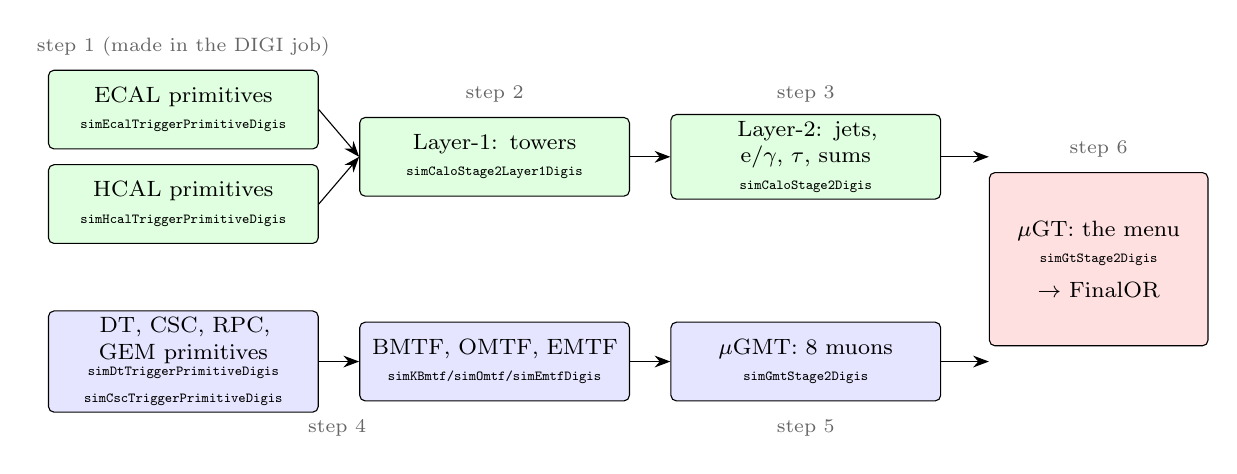
\begin{tikzpicture}[x=0.93cm, font=\footnotesize, >={Stealth[length=2mm]},
  box/.style={draw, rounded corners=2pt, minimum height=10mm, text width=3.25cm, align=center, inner sep=2.5pt},
  calo/.style={box, fill=green!12}, mu/.style={box, fill=blue!10}, gt/.style={box, fill=red!12, text width=2.6cm, minimum height=22mm}]
\node[calo] (etp) at (0,1.75) {ECAL primitives\\{\tiny\ttfamily simEcalTriggerPrimitiveDigis}};
\node[calo] (htp) at (0,0.55) {HCAL primitives\\{\tiny\ttfamily simHcalTriggerPrimitiveDigis}};
\node[calo] (l1) at (4.25,1.15) {Layer-1: towers\\{\tiny\ttfamily simCaloStage2Layer1Digis}};
\node[calo] (l2) at (8.5,1.15) {Layer-2: jets, e/$\gamma$, $\tau$, sums\\{\tiny\ttfamily simCaloStage2Digis}};
\node[mu] (mtp) at (0,-1.45) {DT, CSC, RPC, GEM primitives\\{\tiny\ttfamily simDtTriggerPrimitiveDigis\\simCscTriggerPrimitiveDigis}};
\node[mu] (tf) at (4.25,-1.45) {BMTF, OMTF, EMTF\\{\tiny\ttfamily simKBmtf/simOmtf/simEmtfDigis}};
\node[mu] (gmt) at (8.5,-1.45) {$\mu$GMT: 8 muons\\{\tiny\ttfamily simGmtStage2Digis}};
\node[gt] (ugt) at (12.5,-0.15) {$\mu$GT: the menu\\{\tiny\ttfamily simGtStage2Digis}\\[3pt]$\rightarrow$ FinalOR};
\draw[->] (etp.east) -- (l1.west); \draw[->] (htp.east) -- (l1.west);
\draw[->] (l1) -- (l2); \draw[->] (l2.east) -- (ugt.west|-l2.east);
\draw[->] (mtp) -- (tf); \draw[->] (tf) -- (gmt); \draw[->] (gmt.east) -- (ugt.west|-gmt.east);
\node[font=\scriptsize, text=black!60] at (0,2.55) {step 1 (made in the DIGI job)};
\node[font=\scriptsize, text=black!60] at (4.25,1.95) {step 2};
\node[font=\scriptsize, text=black!60] at (8.5,1.95) {step 3};
\node[font=\scriptsize, text=black!60] at (2.1,-2.3) {step 4};
\node[font=\scriptsize, text=black!60] at (8.5,-2.3) {step 5};
\node[font=\scriptsize, text=black!60] at (12.5,1.25) {step 6};
\end{tikzpicture}
\caption{The Level-1 trigger of Run~3 (the ``stage-2'' trigger, in place since 2016) and the modules of the
\code{SimL1Emulator} sequence that emulate it. Calorimeter chain in green, muon chain in blue.}
\label{fig:12_chain}
\end{figure}

\begin{table}[!htb]
\centering\small\setlength{\tabcolsep}{4pt}
\caption{The six steps at a glance: what each one sends to the next, and how much of it there is in our event.
Every arrow of figure~\ref{fig:12_chain} is a reduction.}
\label{tab:12_glance}
\begin{tabular}{@{}c>{\raggedright\arraybackslash}p{3.2cm}>{\raggedright\arraybackslash}p{6.9cm}>{\raggedright\arraybackslash}p{4.3cm}@{}}
\toprule
step & who & sends, every 25\,ns & in our event \\
\midrule
1 & calorimeter front-ends & 8856 primitives: an 8-bit $E_{\mathrm T}$ and a few flag bits per tower & 2479 above zero, $2793\GeV$ \\
2 & Layer-1 & 5760 tower words of 16 bits: 9-bit $E_{\mathrm T}$, E/H ratio, flags & 2561 above zero, $2181\GeV$ \\
3 & Layer-2 & at most 12 jets, 12 e/$\gamma$, 12 $\tau$, and the energy sums & 9, 12, 12 \\
4 & muon chambers, track finders & stubs; then at most 3 candidates from each of 36 processors & 8 CSC stubs, 2 candidates \\
5 & $\mu$GMT & at most 8 muons & 1 \\
6 & $\mu$GT & 512 algorithm bits and their OR & 63 bits set, FinalOR 1 \\
\bottomrule
\end{tabular}
\end{table}

The chapter has one section per step. Each says what the step receives, what it does, with which parameters, what
the numbers of our event are, and shows the event in $\eta$--$\phi$ as it looks after the step. \emph{One} event is
followed (\path{test/12_L1T/run_12_L1T.sh}): the event as CMS sees it, the signal with the 71, 68 and 54 collisions
of bunch crossings $-1$, 0 and $+1$ on top. Chapter~\ref{ch:11_DIGI} was the last stage at which the signal and
the pileup existed apart; a trigger, like a detector, is only ever given their sum. Where the chapter needs to know
who made an object, it asks the truth that the file still carries: the two generator jets of
chapter~\ref{ch:07_GenJet}, and the simulated particles behind a muon.

\section{From the previous chapter}

One file of chapter~\ref{ch:11_DIGI} enters (Rule E), \path{test/11_DIGI/out/step3_DIGI_mixed_11_DIGI.root}: the
$544\,407$ digis of the signal with its pileup. The L1T uses very little of them. Of the $514\,881$ tracker digis it
uses none. Of the calorimeters it does not read the zero-suppressed data frames at all, but the two collections
that the \code{DIGI} job made from the unsuppressed frames for exactly this purpose,
\code{simEcalTriggerPrimitiveDigis} and \code{simHcalTriggerPrimitiveDigis}: section~\ref{sec:11_tp} of
chapter~\ref{ch:11_DIGI} explained what they are, how they are made and why they are made there. Step~1 of this
chapter was therefore computed in the previous job, and this is why \code{-s L1} cannot run on its own without two
extra lines (the companion, section~1). Of the muon system it uses the wire, strip and pad digis, 2016 of them.

What that section established, in four lines. The trigger sees the calorimeters on a grid of trigger towers,
$i\eta=\pm1\ldots\pm41$ and $i\phi=1\ldots72$ ($|i\eta|\leq17$ barrel, 18 to 28 endcap, 30 to 41 HF, 29 unused),
one 8-bit transverse energy per tower and bunch crossing, $0.5\GeV$ per count. A primitive measures the energy
deposited in its tower to half a GeV, but a tower with less than that sends nothing, and noise alone makes one
tower in nine send a count. Of the $2793\GeV$ of primitives of our event, the signal alone would have sent
$536.5\GeV$, more than half of it noise: four fifths of what the trigger receives is pileup and noise.\footnote{All numbers of this chapter are in
\path{test/12_L1T/out/}: \path{ledger_12_L1T.txt} (step by step), \path{l1t_12_L1T.log} (the analyzers
\code{L1TCaloAnalyzer}, \code{L1TMuonAnalyzer}, \code{L1TGlobalAnalyzer}), \path{settings_12_L1T.txt} (the module
parameters) and \path{truth_12_L1T.txt}; the companion lists them. Numbers about the signal alone are quoted from
chapter~\ref{ch:11_DIGI}.}

The job runs with the 2025 settings of the release: the menu of the global tag is
\path{L1Menu_Collisions2025_v1_0_0}, the ECAL primitives of chapter~\ref{ch:11_DIGI} were made with the payloads of 2025, and the era \code{Run3\_2025}
brings the CICADA model of 2025; the calorimeter-trigger parameters of Layer-1 and Layer-2 and the muon payloads are
those of 2024. The first version of this chapter ran with the 2024 settings; what the
change did to the decision is told in the ledger section.

What is kept: everything. The \code{L1} process copies its input and adds its products under the process name
\code{L1}, about fifty collections, the output of every board of figure~\ref{fig:12_chain}. What changes is the
granularity at which the event is looked at: half a million digis become, for the trigger, 8856 small integers.

\section{Step 1: the calorimeter trigger primitives}

\textbf{What the step does.} Every 25\,ns each calorimeter front-end sends one transverse energy per trigger tower
to Layer-1 on optical links: 4032 from the ECAL, 4032 from HB and HE, 792 from the HF. The primitive of a tower is
a small time series (five consecutive crossings for the ECAL, four for the HCAL), and the trigger takes one value
per crossing: for our event the one of bunch crossing 0, the \emph{sample of interest}. The emulator of the
calorimeter trigger processes this crossing only (\path{L1Trigger/L1TCaloLayer1/plugins/L1TCaloLayer1.cc}: ``Currently
we only read and process the `hit' BX only''); in the detector the crossings $-1$ and $+1$, with their 71 and 54
collisions, go through the same six steps as events of their own.

\textbf{The numbers of the event.} Table~\ref{tab:12_tp} counts what arrives, and figure~\ref{fig:12_tp} shows it.

\begin{table}[!htb]
\centering\small
\caption{Step 1: the trigger primitives of bunch crossing 0 (\code{ledger\_12\_L1T.txt}, section 1).}
\label{tab:12_tp}
\begin{tabular}{l rrrr}
\toprule
 & primitives & with $E_{\mathrm T}>0$ & $\sum E_{\mathrm T}$ [GeV] & largest [GeV] \\
\midrule
ECAL barrel (EB), $|i\eta|\leq17$ & 2448 & 683 & 468.0 & 5.5 \\
ECAL endcap (EE), $18\leq|i\eta|\leq28$ & 1584 & 494 & 579.5 & 7.0 \\
HCAL barrel (HB), $|i\eta|\leq16$ & 2304 & 233 & 183.0 & 7.5 \\
HCAL endcap (HE), $17\leq|i\eta|\leq28$ & 1728 & 328 & 241.5 & 10.0 \\
HF, $30\leq|i\eta|\leq41$ & 792 & 741 & 1321.0 & 90.5 \\
\midrule
all & 8856 & 2479 & 2793.0 & 90.5 \\
\bottomrule
\end{tabular}
\end{table}

\emph{Where the energy is.} Two thirds of it are in two places: the HF ($1321\GeV$, 741 of its 792 primitives
are lit) and the endcap ECAL ($579.5\GeV$). The barrel, with more than half of the towers, holds $651\GeV$. The
pileup is roughly flat in $\eta$, the towers are not: a tower at the edge of the endcap is four times larger than
a barrel tower and collects several soft particles where a barrel tower collects a fraction of one, so that the
half-GeV count that hides most of the pileup in the barrel does not hide it there. In figure~\ref{fig:12_tp} the
rings at $2.5<\abseta<3$ of the ECAL and the whole HF are bands of one to a few GeV per tower, and the barrel a dust
of one- and two-count towers, many of them noise.

\emph{The two jets look completely different.} The $\bar b$ jet ($\pt=115.9\GeV$ at $\eta=-3.75$) falls in the
HF, where a jet is narrow in tower units: one primitive at $i\eta=-34$ carries $90.5\GeV$ and its neighbour at
$i\eta=-33$ another $15.5\GeV$; the $9\times9$ towers around it hold $199.75\GeV$. The $b$ jet sits on the
barrel--endcap boundary, $\eta=-1.59$, and is spread over a dozen towers (figure~\ref{fig:12_tpzoom}): a column of
ECAL towers at $i\eta=-19$ with $7.0$, $6.0$ and $5.0\GeV$ and three HCAL towers with $10.0$, $4.5$ and
$3.5\GeV$; no tower of either calorimeter is above $10\GeV$. Its generator jet has $117.8\GeV$, of which
$37.5\GeV$ are the neutrino of the semileptonic $B^-$ decay of chapter~\ref{ch:06_Decay}; what a calorimeter can
see at best is the $79.8\GeV$ of chapter~\ref{ch:07_GenJet}. In the $9\times9$ towers around it the ECAL
primitives add up to $46.0\GeV$ and the HCAL ones to $28.0\GeV$, pileup included. The jet that the trigger will
build is still visible in figure~\ref{fig:12_tp} only because it is in a quiet region of the detector.

\begin{figure}[!htb]
\centering
\includegraphics[width=0.47\textwidth,trim=0 0 475 0,clip]{12_L1T/out/l1t_12_L1T_calo_ecaltp_run1_event1.png}\hfill
\includegraphics[width=0.47\textwidth,trim=0 0 475 0,clip]{12_L1T/out/l1t_12_L1T_calo_hcaltp_run1_event1.png}
\caption{Step 1, the trigger primitives of the event on the trigger-tower grid, one coloured cell per tower, colour
= $E_{\mathrm T}$ on a logarithmic scale from $0.25$ to $256\GeV$
(\code{l1t\_12\_L1T\_calo\_ecaltp/hcaltp\_run1\_event1.png}). Left: ECAL; right: HCAL, with the HF beyond
$\abseta=3$. Magenta circles: the two \code{ak4GenJets} of chapter~\ref{ch:07_GenJet}. The dotted lines are the
barrel--endcap and endcap--HF boundaries.}
\label{fig:12_tp}
\end{figure}

\begin{figure}[!htb]
\centering
\includegraphics[width=0.47\textwidth,trim=0 0 475 0,clip]{12_L1T/out/l1t_12_L1T_calo_jet2_ecaltp_run1_event1.png}\hfill
\includegraphics[width=0.47\textwidth,trim=0 0 475 0,clip]{12_L1T/out/l1t_12_L1T_calo_jet2_hcaltp_run1_event1.png}
\caption{Step 1, the $b$ jet tower by tower: the ECAL primitives (left) and the HCAL primitives (right) of the
$17\times17$ towers around $(i\eta,i\phi)=(-18,50)$, one square per tower with its $E_{\mathrm T}$ in GeV
(\code{l1t\_12\_L1T\_calo\_jet2\_ecaltp/hcaltp\_run1\_event1.png}). The red square is the $9\times9$ window that step~3
will use; it holds $46.0\GeV$ of ECAL and $28.0\GeV$ of HCAL primitives. The towers outside the jet are the pileup
and the noise.}
\label{fig:12_tpzoom}
\end{figure}

\section{Step 2: calorimeter Layer-1}

\textbf{What the step does.} Layer-1 (18 processing cards in the hardware, the classes \code{UCTLayer1},
\code{UCTCard}, \code{UCTRegion}, \code{UCTTower} of \path{L1Trigger/L1TCaloLayer1} in the emulator) does three
things to every tower. It \emph{receives} the two primitives of the tower and aligns them in time. It
\emph{calibrates} each with a lookup table addressed by the 8-bit value and the tower ring: the table multiplies
the transverse energy by a scale factor that depends on $|i\eta|$ and on the energy, in 14 energy bins from below
$3\GeV$ to above $70\GeV$. And it \emph{sums} the calibrated ECAL and HCAL values into one tower word of 16 bits:
9 bits of $E_{\mathrm T}$ ($0.5\GeV$ per count, saturating at $255.5\GeV$), 3 bits for the ratio of the two
energies on a logarithmic scale, and flag bits (which of the two is larger, the ECAL fine-grain bit, an HCAL
feature bit). The towers of a ring are then sorted and sent to Layer-2. It is the first place where the ECAL and
the HCAL energy of the same $\eta$--$\phi$ cell meet. The scale factors are not in the configuration: they are the
payload \code{L1TCaloParams\_static\_2024\_v0\_1\_mc} of the record \code{L1TCaloParamsRcd} in the global tag, the same
numbers as \path{L1Trigger/L1TCalorimeter/python/caloParams_2024_v0_1_cfi.py}; the analyzer prints the three tables
(companion, section~4).

\textbf{The parameters.} Table~\ref{tab:12_sf} is what the tables do. For the ECAL the factor is a calibration,
$1.12$ at low energy falling to $1.01$ at high energy, with one exception: it is \emph{zero} for the three last
rings of the endcap below a threshold ($3\GeV$ for ring 26, $6\GeV$ for 27, $9\GeV$ for 28). For the HCAL it is 1
everywhere, except that one-count primitives ($0.5\GeV$) are set to zero for $|i\eta|\leq15$ (the comment in the
python file reads ``ZERO-SUPPRESS $<$1GeV (i.e. 0.5GeV) IN THE BARREL ONLY''). For the HF it is 1, but the
primitive is divided between the two (or four) $5^\circ$ towers it covers, each getting half (a quarter) of it
\emph{rounded down} to half a GeV (\path{L1Trigger/L1TCaloLayer1/src/L1TCaloLayer1FetchLUTs.cc}: ``Divide by two
(since two duplicate towers are sent)''), so that a one-count HF primitive disappears. Three zero suppressions,
then, hidden in what is called a calibration, each aimed at the pileup and the noise of step~1.

\begin{table}[!htb]
\centering\small\setlength{\tabcolsep}{4.5pt}
\caption{Step 2: the Layer-1 scale factors of the global tag (\code{l1t\_12\_L1T.log}, lines
\code{caloParams layer1...ScaleFactors}), for some rings and three of the 14 bins of the primitive's $E_{\mathrm T}$.}
\label{tab:12_sf}
\begin{tabular}{l ccccccc}
\toprule
ring $|i\eta|$ & 1 & 15 & 17 & 18 & 25 & 26 / 27 / 28 & 30--41 (HF) \\
\midrule
ECAL, $E_{\mathrm T}<3\GeV$ & 1.12 & 1.13 & 1.14 & 1.26 & 1.19 & 0 / 0 / 0 & \\
ECAL, $6<E_{\mathrm T}<9\GeV$ & 1.08 & 1.10 & 1.10 & 1.23 & 1.15 & 1.14 / 1.14 / 0 & \\
ECAL, $E_{\mathrm T}>70\GeV$ & 1.02 & 1.02 & 1.02 & 1.04 & 1.02 & 1.02 / 1.00 / 1.01 & \\
HCAL, $E_{\mathrm T}<1\GeV$ & 0 & 0 & 1 & 1 & 1 & 1 / 1 / 1 & 1, then $\div2$ ($\div4$) \\
HCAL, $E_{\mathrm T}\geq1\GeV$ & 1 & 1 & 1 & 1 & 1 & 1 / 1 / 1 & 1, then $\div2$ ($\div4$) \\
\bottomrule
\end{tabular}
\end{table}

\textbf{The numbers of the event.} The step removes a fifth of what it receives (table~\ref{tab:12_l1}): $307\GeV$
of the $1047.5\GeV$ of ECAL primitives and $226\GeV$ of the $1321\GeV$ of the HF. Figure~\ref{fig:12_rings} shows
where, ring by ring. The ECAL loss is all in the last three rings of the endcap: rings 26 to 28 receive
$445.5\GeV$, $321.5\GeV$ of it from the ECAL, and come out with $134.5\GeV$. In rings 27 and 28 not one ECAL
primitive reaches the 6 and $9\GeV$ of table~\ref{tab:12_sf}, and only the HCAL is left (the ring $i\eta=+28$
receives $68\GeV$ of ECAL and $36\GeV$ of HCAL primitives and keeps $36\GeV$). The HF loses a little in every ring,
to the rounding. The barrel and the rest of the endcap are hardly touched: the barrel rings receive $655\GeV$ and
keep $576.5\GeV$. After the step the event is 2561 towers and $2181\GeV$, and the bright bands of
figure~\ref{fig:12_l1} are the HF. With the 2024 conditions they were not alone: the ECAL primitives of ring~28 were
four times larger ($315\GeV$ in ring $+28$, up to $11.5\GeV$ each), many survived the $9\GeV$ cut, the ring kept
$181\GeV$, and step~3 seeded six pileup jets in it. The crystals of ring~28 have lost transparency: the 2025
digitiser scales their light by 0.025 instead of 0.096 (chapter~\ref{ch:11_DIGI}), and the larger linearisation
constants of the 2025 primitives ($\times1.37$ there) give back only part of it: per GeV deposited, a ring-28
primitive is 0.36 of what it was in 2024 (0.94 to 0.99 up to ring 23; companion, last section).

\begin{table}[!htb]
\centering\small
\caption{Step 2: what Layer-1 makes of the primitives, summed transverse energy in GeV in and out of the step
(\code{ledger\_12\_L1T.txt}, sections 1 and 2).}
\label{tab:12_l1}
\begin{tabular}{l rrr c l rr}
\toprule
 & in & out & change & & towers after the step & $E_{\mathrm T}>0$ & $\sum E_{\mathrm T}$ \\
\cmidrule(lr){1-4}\cmidrule(lr){6-8}
ECAL (EB + EE) & 1047.5 & 740.5 & $-307.0$ & & barrel, $|i\eta|\leq17$ & 738 & 576.5 \\
HCAL (HB + HE) & 424.5 & 345.5 & $-79.0$ & & endcap, $18\leq|i\eta|\leq28$ & 557 & 509.5 \\
HF & 1321.0 & 1095.0 & $-226.0$ & & forward, $|i\eta|\geq30$ & 1266 & 1095.0 \\
all & 2793.0 & 2181.0 & $-612.0$ & & all (of 5760) & 2561 & 2181.0 \\
\bottomrule
\end{tabular}
\end{table}

\begin{figure}[!htb]
\centering
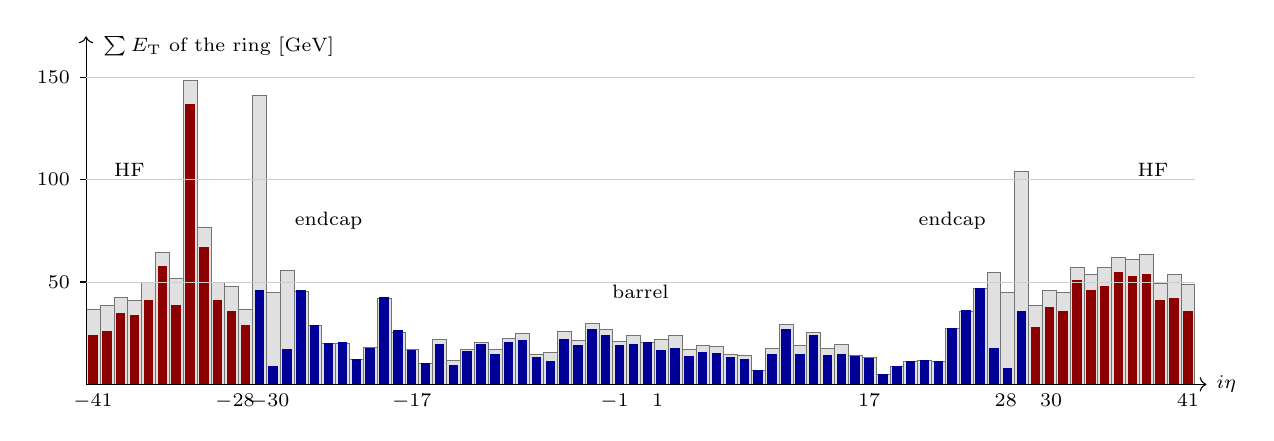
\begin{tikzpicture}[x=1cm, y=0.026cm, font=\scriptsize]
\draw[black!55, fill=black!12, line width=0.2pt] (0.000,0) rectangle (0.176,36.5);
\fill[red!55!black] (0.028,0) rectangle (0.148,24.0);
\draw[black!55, fill=black!12, line width=0.2pt] (0.176,0) rectangle (0.352,38.5);
\fill[red!55!black] (0.204,0) rectangle (0.324,26.0);
\draw[black!55, fill=black!12, line width=0.2pt] (0.352,0) rectangle (0.528,42.5);
\fill[red!55!black] (0.380,0) rectangle (0.500,35.0);
\draw[black!55, fill=black!12, line width=0.2pt] (0.528,0) rectangle (0.704,41.0);
\fill[red!55!black] (0.556,0) rectangle (0.676,34.0);
\draw[black!55, fill=black!12, line width=0.2pt] (0.704,0) rectangle (0.880,50.0);
\fill[red!55!black] (0.732,0) rectangle (0.852,41.0);
\draw[black!55, fill=black!12, line width=0.2pt] (0.880,0) rectangle (1.056,64.5);
\fill[red!55!black] (0.908,0) rectangle (1.028,58.0);
\draw[black!55, fill=black!12, line width=0.2pt] (1.056,0) rectangle (1.232,52.0);
\fill[red!55!black] (1.084,0) rectangle (1.204,39.0);
\draw[black!55, fill=black!12, line width=0.2pt] (1.232,0) rectangle (1.408,148.5);
\fill[red!55!black] (1.260,0) rectangle (1.380,137.0);
\draw[black!55, fill=black!12, line width=0.2pt] (1.408,0) rectangle (1.584,76.5);
\fill[red!55!black] (1.436,0) rectangle (1.556,67.0);
\draw[black!55, fill=black!12, line width=0.2pt] (1.584,0) rectangle (1.760,50.0);
\fill[red!55!black] (1.612,0) rectangle (1.732,41.0);
\draw[black!55, fill=black!12, line width=0.2pt] (1.760,0) rectangle (1.936,48.0);
\fill[red!55!black] (1.788,0) rectangle (1.908,36.0);
\draw[black!55, fill=black!12, line width=0.2pt] (1.936,0) rectangle (2.112,36.5);
\fill[red!55!black] (1.964,0) rectangle (2.084,29.0);
\draw[black!55, fill=black!12, line width=0.2pt] (2.112,0) rectangle (2.288,141.0);
\fill[blue!60!black] (2.140,0) rectangle (2.260,46.0);
\draw[black!55, fill=black!12, line width=0.2pt] (2.288,0) rectangle (2.464,45.0);
\fill[blue!60!black] (2.316,0) rectangle (2.436,9.0);
\draw[black!55, fill=black!12, line width=0.2pt] (2.464,0) rectangle (2.640,55.5);
\fill[blue!60!black] (2.492,0) rectangle (2.612,17.5);
\draw[black!55, fill=black!12, line width=0.2pt] (2.640,0) rectangle (2.816,45.5);
\fill[blue!60!black] (2.668,0) rectangle (2.788,46.0);
\draw[black!55, fill=black!12, line width=0.2pt] (2.816,0) rectangle (2.992,29.0);
\fill[blue!60!black] (2.844,0) rectangle (2.964,29.0);
\draw[black!55, fill=black!12, line width=0.2pt] (2.992,0) rectangle (3.168,20.0);
\fill[blue!60!black] (3.020,0) rectangle (3.140,20.0);
\draw[black!55, fill=black!12, line width=0.2pt] (3.168,0) rectangle (3.344,20.0);
\fill[blue!60!black] (3.196,0) rectangle (3.316,20.5);
\draw[black!55, fill=black!12, line width=0.2pt] (3.344,0) rectangle (3.520,12.5);
\fill[blue!60!black] (3.372,0) rectangle (3.492,12.5);
\draw[black!55, fill=black!12, line width=0.2pt] (3.520,0) rectangle (3.696,18.0);
\fill[blue!60!black] (3.548,0) rectangle (3.668,18.0);
\draw[black!55, fill=black!12, line width=0.2pt] (3.696,0) rectangle (3.872,42.0);
\fill[blue!60!black] (3.724,0) rectangle (3.844,42.5);
\draw[black!55, fill=black!12, line width=0.2pt] (3.872,0) rectangle (4.048,25.5);
\fill[blue!60!black] (3.900,0) rectangle (4.020,26.5);
\draw[black!55, fill=black!12, line width=0.2pt] (4.048,0) rectangle (4.224,17.0);
\fill[blue!60!black] (4.076,0) rectangle (4.196,17.0);
\draw[black!55, fill=black!12, line width=0.2pt] (4.224,0) rectangle (4.400,10.5);
\fill[blue!60!black] (4.252,0) rectangle (4.372,10.5);
\draw[black!55, fill=black!12, line width=0.2pt] (4.400,0) rectangle (4.576,22.0);
\fill[blue!60!black] (4.428,0) rectangle (4.548,19.5);
\draw[black!55, fill=black!12, line width=0.2pt] (4.576,0) rectangle (4.752,12.0);
\fill[blue!60!black] (4.604,0) rectangle (4.724,9.5);
\draw[black!55, fill=black!12, line width=0.2pt] (4.752,0) rectangle (4.928,17.0);
\fill[blue!60!black] (4.780,0) rectangle (4.900,16.5);
\draw[black!55, fill=black!12, line width=0.2pt] (4.928,0) rectangle (5.104,20.5);
\fill[blue!60!black] (4.956,0) rectangle (5.076,19.5);
\draw[black!55, fill=black!12, line width=0.2pt] (5.104,0) rectangle (5.280,17.0);
\fill[blue!60!black] (5.132,0) rectangle (5.252,15.0);
\draw[black!55, fill=black!12, line width=0.2pt] (5.280,0) rectangle (5.456,22.5);
\fill[blue!60!black] (5.308,0) rectangle (5.428,20.5);
\draw[black!55, fill=black!12, line width=0.2pt] (5.456,0) rectangle (5.632,25.0);
\fill[blue!60!black] (5.484,0) rectangle (5.604,21.5);
\draw[black!55, fill=black!12, line width=0.2pt] (5.632,0) rectangle (5.808,14.5);
\fill[blue!60!black] (5.660,0) rectangle (5.780,13.5);
\draw[black!55, fill=black!12, line width=0.2pt] (5.808,0) rectangle (5.984,15.5);
\fill[blue!60!black] (5.836,0) rectangle (5.956,11.5);
\draw[black!55, fill=black!12, line width=0.2pt] (5.984,0) rectangle (6.160,26.0);
\fill[blue!60!black] (6.012,0) rectangle (6.132,22.0);
\draw[black!55, fill=black!12, line width=0.2pt] (6.160,0) rectangle (6.336,21.5);
\fill[blue!60!black] (6.188,0) rectangle (6.308,19.0);
\draw[black!55, fill=black!12, line width=0.2pt] (6.336,0) rectangle (6.512,30.0);
\fill[blue!60!black] (6.364,0) rectangle (6.484,27.0);
\draw[black!55, fill=black!12, line width=0.2pt] (6.512,0) rectangle (6.688,27.0);
\fill[blue!60!black] (6.540,0) rectangle (6.660,24.0);
\draw[black!55, fill=black!12, line width=0.2pt] (6.688,0) rectangle (6.864,21.0);
\fill[blue!60!black] (6.716,0) rectangle (6.836,19.0);
\draw[black!55, fill=black!12, line width=0.2pt] (6.864,0) rectangle (7.040,24.0);
\fill[blue!60!black] (6.892,0) rectangle (7.012,19.5);
\draw[black!55, fill=black!12, line width=0.2pt] (7.040,0) rectangle (7.216,20.5);
\fill[blue!60!black] (7.068,0) rectangle (7.188,20.5);
\draw[black!55, fill=black!12, line width=0.2pt] (7.216,0) rectangle (7.392,22.0);
\fill[blue!60!black] (7.244,0) rectangle (7.364,17.0);
\draw[black!55, fill=black!12, line width=0.2pt] (7.392,0) rectangle (7.568,24.0);
\fill[blue!60!black] (7.420,0) rectangle (7.540,18.0);
\draw[black!55, fill=black!12, line width=0.2pt] (7.568,0) rectangle (7.744,17.0);
\fill[blue!60!black] (7.596,0) rectangle (7.716,14.0);
\draw[black!55, fill=black!12, line width=0.2pt] (7.744,0) rectangle (7.920,19.0);
\fill[blue!60!black] (7.772,0) rectangle (7.892,16.0);
\draw[black!55, fill=black!12, line width=0.2pt] (7.920,0) rectangle (8.096,18.5);
\fill[blue!60!black] (7.948,0) rectangle (8.068,15.5);
\draw[black!55, fill=black!12, line width=0.2pt] (8.096,0) rectangle (8.272,14.5);
\fill[blue!60!black] (8.124,0) rectangle (8.244,13.5);
\draw[black!55, fill=black!12, line width=0.2pt] (8.272,0) rectangle (8.448,14.0);
\fill[blue!60!black] (8.300,0) rectangle (8.420,12.5);
\draw[black!55, fill=black!12, line width=0.2pt] (8.448,0) rectangle (8.624,7.0);
\fill[blue!60!black] (8.476,0) rectangle (8.596,7.0);
\draw[black!55, fill=black!12, line width=0.2pt] (8.624,0) rectangle (8.800,17.5);
\fill[blue!60!black] (8.652,0) rectangle (8.772,15.0);
\draw[black!55, fill=black!12, line width=0.2pt] (8.800,0) rectangle (8.976,29.5);
\fill[blue!60!black] (8.828,0) rectangle (8.948,27.0);
\draw[black!55, fill=black!12, line width=0.2pt] (8.976,0) rectangle (9.152,19.0);
\fill[blue!60!black] (9.004,0) rectangle (9.124,15.0);
\draw[black!55, fill=black!12, line width=0.2pt] (9.152,0) rectangle (9.328,25.5);
\fill[blue!60!black] (9.180,0) rectangle (9.300,24.0);
\draw[black!55, fill=black!12, line width=0.2pt] (9.328,0) rectangle (9.504,17.5);
\fill[blue!60!black] (9.356,0) rectangle (9.476,14.5);
\draw[black!55, fill=black!12, line width=0.2pt] (9.504,0) rectangle (9.680,19.5);
\fill[blue!60!black] (9.532,0) rectangle (9.652,15.0);
\draw[black!55, fill=black!12, line width=0.2pt] (9.680,0) rectangle (9.856,14.0);
\fill[blue!60!black] (9.708,0) rectangle (9.828,14.0);
\draw[black!55, fill=black!12, line width=0.2pt] (9.856,0) rectangle (10.032,13.0);
\fill[blue!60!black] (9.884,0) rectangle (10.004,13.0);
\draw[black!55, fill=black!12, line width=0.2pt] (10.032,0) rectangle (10.208,5.0);
\fill[blue!60!black] (10.060,0) rectangle (10.180,5.0);
\draw[black!55, fill=black!12, line width=0.2pt] (10.208,0) rectangle (10.384,9.0);
\fill[blue!60!black] (10.236,0) rectangle (10.356,9.0);
\draw[black!55, fill=black!12, line width=0.2pt] (10.384,0) rectangle (10.560,11.5);
\fill[blue!60!black] (10.412,0) rectangle (10.532,11.5);
\draw[black!55, fill=black!12, line width=0.2pt] (10.560,0) rectangle (10.736,12.0);
\fill[blue!60!black] (10.588,0) rectangle (10.708,12.0);
\draw[black!55, fill=black!12, line width=0.2pt] (10.736,0) rectangle (10.912,11.5);
\fill[blue!60!black] (10.764,0) rectangle (10.884,11.5);
\draw[black!55, fill=black!12, line width=0.2pt] (10.912,0) rectangle (11.088,27.5);
\fill[blue!60!black] (10.940,0) rectangle (11.060,27.5);
\draw[black!55, fill=black!12, line width=0.2pt] (11.088,0) rectangle (11.264,35.5);
\fill[blue!60!black] (11.116,0) rectangle (11.236,36.5);
\draw[black!55, fill=black!12, line width=0.2pt] (11.264,0) rectangle (11.440,47.0);
\fill[blue!60!black] (11.292,0) rectangle (11.412,47.0);
\draw[black!55, fill=black!12, line width=0.2pt] (11.440,0) rectangle (11.616,55.0);
\fill[blue!60!black] (11.468,0) rectangle (11.588,18.0);
\draw[black!55, fill=black!12, line width=0.2pt] (11.616,0) rectangle (11.792,45.0);
\fill[blue!60!black] (11.644,0) rectangle (11.764,8.0);
\draw[black!55, fill=black!12, line width=0.2pt] (11.792,0) rectangle (11.968,104.0);
\fill[blue!60!black] (11.820,0) rectangle (11.940,36.0);
\draw[black!55, fill=black!12, line width=0.2pt] (11.968,0) rectangle (12.144,38.5);
\fill[red!55!black] (11.996,0) rectangle (12.116,28.0);
\draw[black!55, fill=black!12, line width=0.2pt] (12.144,0) rectangle (12.320,46.0);
\fill[red!55!black] (12.172,0) rectangle (12.292,38.0);
\draw[black!55, fill=black!12, line width=0.2pt] (12.320,0) rectangle (12.496,45.0);
\fill[red!55!black] (12.348,0) rectangle (12.468,36.0);
\draw[black!55, fill=black!12, line width=0.2pt] (12.496,0) rectangle (12.672,57.0);
\fill[red!55!black] (12.524,0) rectangle (12.644,51.0);
\draw[black!55, fill=black!12, line width=0.2pt] (12.672,0) rectangle (12.848,54.0);
\fill[red!55!black] (12.700,0) rectangle (12.820,46.0);
\draw[black!55, fill=black!12, line width=0.2pt] (12.848,0) rectangle (13.024,57.0);
\fill[red!55!black] (12.876,0) rectangle (12.996,48.0);
\draw[black!55, fill=black!12, line width=0.2pt] (13.024,0) rectangle (13.200,62.0);
\fill[red!55!black] (13.052,0) rectangle (13.172,55.0);
\draw[black!55, fill=black!12, line width=0.2pt] (13.200,0) rectangle (13.376,61.0);
\fill[red!55!black] (13.228,0) rectangle (13.348,53.0);
\draw[black!55, fill=black!12, line width=0.2pt] (13.376,0) rectangle (13.552,63.5);
\fill[red!55!black] (13.404,0) rectangle (13.524,54.0);
\draw[black!55, fill=black!12, line width=0.2pt] (13.552,0) rectangle (13.728,49.5);
\fill[red!55!black] (13.580,0) rectangle (13.700,41.0);
\draw[black!55, fill=black!12, line width=0.2pt] (13.728,0) rectangle (13.904,54.0);
\fill[red!55!black] (13.756,0) rectangle (13.876,42.0);
\draw[black!55, fill=black!12, line width=0.2pt] (13.904,0) rectangle (14.080,49.0);
\fill[red!55!black] (13.932,0) rectangle (14.052,36.0);
\draw[->] (0,0) -- (14.23,0) node[right] {$i\eta$};
\draw[->] (0,0) -- (0,170);
\node[anchor=west] at (0.1,165) {$\sum E_{\mathrm T}$ of the ring [GeV]};
\draw (0,50) -- (-0.08,50) node[left] {50};
\draw[black!20, line width=0.2pt] (0,50) -- (14.08,50);
\draw (0,100) -- (-0.08,100) node[left] {100};
\draw[black!20, line width=0.2pt] (0,100) -- (14.08,100);
\draw (0,150) -- (-0.08,150) node[left] {150};
\draw[black!20, line width=0.2pt] (0,150) -- (14.08,150);
\node[anchor=north, inner sep=1.5pt] at (0.088,-2.5) {$-41$};
\node[anchor=north west, inner sep=1.5pt] at (2.024,-2.5) {$-30$};
\node[anchor=north east, inner sep=1.5pt] at (2.200,-2.5) {$-28$};
\node[anchor=north, inner sep=1.5pt] at (4.136,-2.5) {$-17$};
\node[anchor=north east, inner sep=1.5pt] at (6.952,-2.5) {$-1$};
\node[anchor=north west, inner sep=1.5pt] at (7.128,-2.5) {1};
\node[anchor=north, inner sep=1.5pt] at (9.944,-2.5) {17};
\node[anchor=north east, inner sep=1.5pt] at (11.880,-2.5) {28};
\node[anchor=north west, inner sep=1.5pt] at (12.056,-2.5) {30};
\node[anchor=north, inner sep=1.5pt] at (13.992,-2.5) {41};
\node at (0.55,105) {HF};
\node at (3.08,80) {endcap};
\node at (7.04,45) {barrel};
\node at (11.00,80) {endcap};
\node at (13.55,105) {HF};
\end{tikzpicture}
\caption{Step 2 ring by ring: the summed $E_{\mathrm T}$ of the 72 towers of each $\eta$ ring
(\code{ledger\_12\_L1T.txt}, section 2). Grey: the ECAL + HCAL primitives that enter Layer-1; colour: the towers that
leave it (blue: barrel and endcap, red: HF). The grey above the colour is what the step removes: the low primitives
of ECAL rings 26 to 28, and the rounding of the HF primitives. The two spikes in the HF at $i\eta=-34,-33$ are the
$\bar b$ jet.}
\label{fig:12_rings}
\end{figure}

Figure~\ref{fig:12_hfzoom} shows the step at work on the $\bar b$ jet: the $90.5\GeV$ primitive at $i\eta=-34$
becomes two towers of $45.0\GeV$ side by side in $\phi$, the $15.5\GeV$ one next to it two towers of $7.5\GeV$
(half a GeV is lost in the rounding each time), and every primitive of $0.5\GeV$ vanishes: $199.75\GeV$ of
primitives in the window, $189.0\GeV$ of towers. For the $b$ jet the seed tower $(-18,50)$ becomes
$3.5\times1.26\rightarrow4.0\GeV$ of ECAL plus $10.0\GeV$ of HCAL, a tower of $14.0\GeV$.

\begin{plainwords}[One tower word, bit by bit]
The tower $(-18,50)$ leaves Layer-1 as 16 bits (\path{L1Trigger/L1TCaloLayer1/src/UCTTower.cc}). Bits 0 to 8:
$E_{\mathrm T}=28$ counts, $14.0\GeV$, the sum of 8 counts of ECAL and 20 of HCAL. Bits 9 to 11: the ratio code 1,
the difference of the two energies in powers of two ($\log_2 20=4$, $\log_2 8=3$). Bit 12, ``one of the two is
zero'': 0. Bit 13, ``the ECAL is the larger'': 0, this tower is hadronic. Bits 14 and 15, the HCAL feature bit and
the ECAL fine-grain bit: 0. Layer-2 never sees the two energies separately: for its jets it uses the first nine
bits, for electrons and photons the ratio and the flags. The tower $(-4,4)$, with $6.0\GeV$ of ECAL and no HCAL,
has bits 12 and 13 set; the HF tower $(-34,11)$ of the $\bar b$ jet, $45.0\GeV$, has bit 12 (an HF tower has no
ECAL) and bit 14, which in the HF means ``above the minimum-bias threshold''.
\end{plainwords}

\begin{figure}[!htb]
\centering
\includegraphics[width=0.47\textwidth,trim=0 0 475 0,clip]{12_L1T/out/l1t_12_L1T_calo_jet1_hcaltp_run1_event1.png}\hfill
\includegraphics[width=0.47\textwidth,trim=0 0 475 0,clip]{12_L1T/out/l1t_12_L1T_calo_jet1_layer1_run1_event1.png}
\caption{Step 2 at work on the $\bar b$ jet, in the HF: the HCAL primitives (left; a primitive is two towers wide
in $\phi$, four for $|i\eta|\geq40$, the grey frames) and the Layer-1 towers made of them (right)
(\code{l1t\_12\_L1T\_calo\_jet1\_hcaltp/layer1\_run1\_event1.png}). Each primitive is shared between its towers and rounded
down to $0.5\GeV$; the black square is the seed tower of step~3, $(i\eta,i\phi)=(-34,12)$, the red one its
$9\times9$ window. The column at $i\eta=-28$, on the right, is the last ring of the endcap.}
\label{fig:12_hfzoom}
\end{figure}

\begin{figure}[!htb]
\centering
\includegraphics[width=0.93\textwidth]{12_L1T/out/l1t_12_L1T_calo_layer1_run1_event1.png}
\caption{Step 2, the Layer-1 towers of the event (ECAL + HCAL, calibrated): 2561 towers, $2181\GeV$
(\code{l1t\_12\_L1T\_calo\_layer1\_run1\_event1.png}). This map is the whole input of step 3.}
\label{fig:12_l1}
\end{figure}

\section{Step 3: calorimeter Layer-2}

\textbf{What the step does.} Layer-2 receives the 5760 tower words of one bunch crossing and runs four algorithms
on them at once (\code{L1TStage2Layer2Producer}; the algorithms are
\path{L1Trigger/L1TCalorimeter/src/firmware/Stage2Layer2*AlgorithmFirmwareImp1.cc}, with the parameters of the same
\code{L1TCaloParamsRcd} payload). The one that matters for this book is the jet algorithm.

\begin{plainwords}[A Level-1 jet in four lines]
(1) \emph{Seed}: any tower of at least $4\GeV$ (\code{jetSeedThreshold = 4}) that is the largest of the
$9\times9$ towers around it (ties are broken by a fixed mask, so that two equal towers cannot both win).
(2) \emph{Window}: the jet is the sum of those 81 towers, $0.78\times0.78$ in $\eta\times\phi$ in the barrel,
comparable to an anti-$k_{\mathrm T}$ jet of radius 0.4.
(3) \emph{Pileup}: take the nine $\eta$ rings the window spans, add up \emph{all 72 towers in $\phi$} of each
ring, and scale to the nine towers of the window, $\times9/72$: this estimate of what a quiet window of the same
$\eta$ contains is subtracted (the ``$\phi$-ring'' subtraction, \code{jetPUSUsePhiRing = 1}). (4)
\emph{Calibration}: the result is multiplied by a factor from a lookup table addressed by its $E_{\mathrm T}$ and
$\eta$ (\code{jetCalibrationType = LUT}). The twelve largest jets, six per $\eta$ side, go to the global trigger.
\end{plainwords}

The $\phi$-ring subtraction is the choice of 2024 and 2025. From 2016 to 2022 the estimate came from the ``chunky donut'', the
three quietest of four $3\times9$ strips around the window; the payload still carries the name
(\code{jetPUSType = ChunkyDonut}) but the flag wins: the method \code{create} of the jet algorithm reads
\code{if (params\_->jetPUSUsePhiRing())} \code{PUSubMethod = "PhiRing1"}. The analyzer recomputes the estimate from the
towers and finds the emulator's value for all nine jets of the event.

The other three algorithms, briefly. \emph{e/$\gamma$}: a seed tower of $2\GeV$ and its neighbours above
$1\GeV$ form a cluster of at most 8 towers, kept if its shape, its HCAL fraction and the fine-grain bit look
electromagnetic, with an isolation bit from the energy around it. \emph{$\tau$}: one or two merged clusters with an
isolation bit; any narrow jet makes one. \emph{Sums}: the total transverse energy (ETT: all towers with
$|i\eta|\leq28$), the missing transverse energy (ETM: the vector sum of the same towers, above a tower threshold
that grows with the number of towers hit, read from \code{metPumLUT\_2023v0\_puppiMet\_fit.txt}; ETMHF: the same with
the HF), and the jet sums HTT and HTM (the scalar and vector sum of the jets above $30\GeV$ with $|i\eta|\leq26$,
that is $\abseta<2.5$; HTMHF with the HF jets).

\textbf{The numbers of the event: the two jets.} Table~\ref{tab:12_jets} follows the two jets of the signal
through the four lines of the box, and figure~\ref{fig:12_zoomb} shows them tower by tower.

\begin{table}[!htb]
\centering\small
\caption{Step 3: the arithmetic of the two signal jets in Layer-2, in GeV (\code{ledger\_12\_L1T.txt}, section 3).
``$\phi$ rings'' is the summed $E_{\mathrm T}$ of the nine rings of the window over all $\phi$. The generator jets
are those of chapter~\ref{ch:07_GenJet}.}
\label{tab:12_jets}
\begin{tabular}{@{}l rr@{}}
\toprule
 & $b$ jet, $\eta=-1.59$ & $\bar b$ jet, $\eta=-3.75$ (HF) \\
\midrule
\code{ak4GenJet} \pt{} (without the neutrino) & 117.8 (79.8) & 115.9 (115.9) \\
seed tower $(i\eta,i\phi)$ & $(-18,50)$ & $(-34,12)$ \\
seed tower & 14.0 & 45.0 \\
$9\times9$ window & 74.5 & 189.0 \\
$\phi$ rings of the window & 176.5 & 482.0 \\
pileup estimate ($\times9/72$) & 22.0 & 60.0 \\
window $-$ pileup & 52.5 & 129.0 \\
calibration factor & 2.07 & 1.05 \\
\textbf{L1 jet $E_{\mathrm T}$} & \textbf{108.5} & \textbf{136.0} \\
L1 jet $\eta$, $\phi$ & $-1.52$, $-1.98$ & $-3.74$, $1.00$ \\
\bottomrule
\end{tabular}
\end{table}

\emph{The $b$ jet.} Its window holds $74.5\GeV$ for a jet of $79.8\GeV$ of visible particles, pileup included: this
is the response of uncalibrated towers at the barrel--endcap boundary. The nine rings of the window hold
$176.5\GeV$, and an eighth of that, $22.0\GeV$, is subtracted. The estimate is not only pileup: the window is part of
its own rings, so that $74.5/8=9.3\GeV$ of the $22.0\GeV$ are the jet subtracted from itself. What is left,
$52.5\GeV$, is two thirds of the visible jet, and the calibration has to repair both the response and the
over-subtraction: a factor 2.07, which lands at $108.5\GeV$. That is $8\,\%$ below the generator jet with its
neutrino and a third above what the calorimeter could see: the lookup table knows the average jet of this
$E_{\mathrm T}$ and $\eta$, not that this one hid $37.5\GeV$ in a neutrino. The direction is that of the centre of
the seed tower, $(\eta,\phi)=(-1.52,-1.98)$, at $\Delta R=0.13$ from the generator jet.

\emph{The $\bar b$ jet.} In the HF the picture is the opposite. The window holds $189.0\GeV$ for a generator jet
of $115.9\GeV$: here most of the excess is pileup, the same towers held $124\GeV$ of primitives without it
(chapter~\ref{ch:11_DIGI}). The rings hold $482\GeV$ and the estimate is $60.0\GeV$; what is left is $129\GeV$,
the calibration is close to one, 1.05, and the jet comes out at $136.0\GeV$, 17\,\% above the truth: the pileup
under this jet was above the average of its rings, and the difference stays in the jet. These $20\GeV$ decide an
algorithm in step~6.

\begin{figure}[!htb]
\centering
\includegraphics[width=0.47\textwidth,trim=0 0 475 0,clip]{12_L1T/out/l1t_12_L1T_calo_jet2_layer1_run1_event1.png}\hfill
\includegraphics[width=0.47\textwidth,trim=0 0 475 0,clip]{12_L1T/out/l1t_12_L1T_calo_jet1_layer1_run1_event1.png}
\caption{Step 3, the two signal jets as the firmware sees them: the Layer-1 towers around the seed, one square per
tower with its $E_{\mathrm T}$ in GeV (\code{l1t\_12\_L1T\_calo\_jet2/jet1\_layer1\_run1\_event1.png}). Left: the $b$
jet, seed $(-18,50)$, window $74.5\GeV$. Right: the $\bar b$ jet in the HF, seed $(-34,12)$, window $189.0\GeV$.
Black: the seed tower; red: the $9\times9$ window; blue: the nine $\eta$ rings of the pileup estimate, which
continue over all 72 towers in $\phi$.}
\label{fig:12_zoomb}
\end{figure}

\begin{figure}[!htb]
\centering
\includegraphics[width=0.93\textwidth]{12_L1T/out/l1t_12_L1T_calo_layer2_run1_event1.png}
\caption{Step 3, the nine Layer-2 jets on the Layer-1 towers (\code{l1t\_12\_L1T\_calo\_layer2\_run1\_event1.png}): red,
the $9\times9$ windows with the jet $E_{\mathrm T}$; blue, the $\phi$ rings of the two leading jets. The two jets
in the magenta circles are the signal; the other seven are pileup and noise.}
\label{fig:12_l2}
\end{figure}

\textbf{The numbers of the event: everything else.} Layer-2 sends 9 jets and full lists of 12 e/$\gamma$ and 12
$\tau$ candidates (figure~\ref{fig:12_l2}, table~\ref{tab:12_alljets}). Seven of the nine jets have no generator jet
behind them: $23.0$, $20.0$, $17.5$, $15.0$, $14.0$, $13.0$ and $9.5\GeV$, four in the barrel and three in the
endcaps, each seeded by a tower of 4 to $7.5\GeV$. Their windows hold 17 to $32.5\GeV$ and their pileup estimates 13 to
$31\GeV$ (the same for all jets of the same $\eta$, as the method wants), so what is left is 1.5 to $7.5\GeV$, and
the calibration, made for real jets whose towers respond low, multiplies it by 3.1 to 6.3
(figure~\ref{fig:12_calib}). The $14.0\GeV$ one, at $(-2.26,-1.80)$, $\Delta R=0.73$ from the $b$ jet, shares part
of its window with it; the others are fluctuations of the pileup and the noise. None is seeded in tower ring 28,
where with the 2024 conditions six of twelve jets were ($12.5$ to $75.5\GeV$). The largest $\tau$ candidate,
$58.5\GeV$ at $(-1.57,-1.93)$, is the core of the $b$ jet; the largest e/$\gamma$ candidate has $7.5\GeV$ and sits
at $(-0.30,0.30)$, on the one barrel tower that chapter~\ref{ch:11_DIGI} found flagged high interest.

\begin{table}[!htb]
\centering\small
\caption{Step 3: the nine jets Layer-2 sends to the global trigger, in GeV (\code{ledger\_12\_L1T.txt}, section 3).}
\label{tab:12_alljets}
\begin{tabular}{rrr c rrrr l}
\toprule
$E_{\mathrm T}$ & $\eta$ & $\phi$ & seed $(i\eta,i\phi)$ & seed & window & pileup & calibration & what it is \\
\midrule
136.0 & $-3.74$ & $1.00$ & $(-34,12)$ & 45.0 & 189.0 & 60.0 & 1.05 & the $\bar b$ jet \\
108.5 & $-1.52$ & $-1.98$ & $(-18,50)$ & 14.0 & 74.5 & 22.0 & 2.07 & the $b$ jet \\
23.0 & $0.91$ & $1.70$ & $(11,20)$ & 7.5 & 25.0 & 17.5 & 3.07 & no generator jet, barrel \\
20.0 & $-0.30$ & $0.30$ & $(-4,4)$ & 6.0 & 28.5 & 22.0 & 3.08 & no generator jet, barrel \\
17.5 & $1.52$ & $0.91$ & $(18,11)$ & 4.0 & 17.0 & 13.0 & 4.38 & no generator jet, endcap \\
15.0 & $0.91$ & $-2.50$ & $(11,44)$ & 4.5 & 21.0 & 17.5 & 4.29 & no generator jet, barrel \\
14.0 & $-2.26$ & $-1.80$ & $(-25,52)$ & 4.0 & 32.5 & 28.5 & 3.50 & next to the $b$ jet \\
13.0 & $1.09$ & $2.74$ & $(13,32)$ & 4.0 & 20.5 & 18.0 & 5.20 & no generator jet, barrel \\
9.5 & $2.39$ & $-1.54$ & $(26,55)$ & 4.0 & 32.5 & 31.0 & 6.33 & no generator jet, endcap \\
\midrule
356.5 & & & & & 440.5 & 229.5 & & all nine \\
\bottomrule
\end{tabular}
\end{table}

\begin{figure}[!htb]
\centering
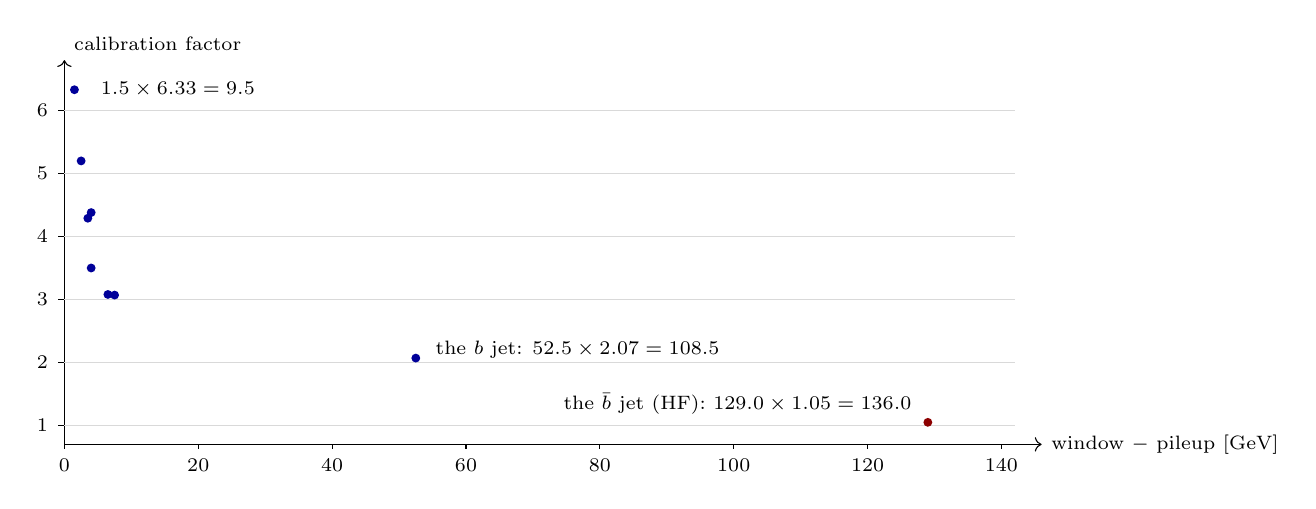
\begin{tikzpicture}[x=0.085cm, y=0.8cm, font=\scriptsize]
\draw[->] (0,0.7) -- (146,0.7) node[right] {window $-$ pileup [GeV]};
\draw[->] (0,0.7) -- (0,6.8) node[above right] {calibration factor};
\foreach \x in {0,20,...,140} \draw (\x,0.7) -- (\x,0.62) node[below] {\x};
\foreach \y in {1,2,3,4,5,6} { \draw (0,\y) -- (-1,\y) node[left] {\y}; \draw[black!15] (0,\y) -- (142,\y); }
\foreach \x/\y in {52.5/2.07, 7.5/3.07, 6.5/3.08, 4/4.38, 3.5/4.29, 4/3.50, 2.5/5.20, 1.5/6.33} \fill[blue!60!black] (\x,\y) circle (1.6pt);
\fill[red!55!black] (129,1.05) circle (1.6pt);
\node[anchor=west] at (54,2.2) {the $b$ jet: $52.5\times2.07=108.5$};
\node[anchor=east] at (128,1.35) {the $\bar b$ jet (HF): $129.0\times1.05=136.0$};
\node[anchor=west] at (4,6.33) {$1.5\times6.33=9.5$};
\end{tikzpicture}
\caption{Step 3, the calibration of the nine jets (table~\ref{tab:12_alljets}): the factor by which Layer-2
multiplies what is left of the window after the pileup subtraction. Blue: barrel and endcap; red: HF. The lookup
table is steep at low energy: a window with $1.5\GeV$ left becomes a jet of $9.5\GeV$.}
\label{fig:12_calib}
\end{figure}


The sums tell the same story in one number each. HTT counts only jets above $30\GeV$ within $\abseta<2.5$, so it
is the $b$ jet alone, $108.5\GeV$: the jet in the HF does not enter it. ETT, the sum of the towers of
barrel and endcap, is $1086\GeV$. The missing transverse energy is real in this event, but small: the neutrino,
$37.5\GeV$ at $\phi=-2.10$ (\code{genMetTrue} of chapter~\ref{ch:06_Decay}). The trigger finds
$\mathrm{ETMHF}=79.0\GeV$ at $\phi=-2.32$, near the neutrino but twice too large: the sum is made of uncalibrated
towers, in which the $b$ jet weighs $74.5\GeV$ and the $\bar b$ jet opposite to it $189\GeV$, and of all the
pileup towers. $\mathrm{HTMHF}$, the same made of the calibrated jets above $30\GeV$, is $34.5\GeV$: the two
signal jets, $136.0$ and $108.5\GeV$ almost back to back. (In 2024 the ring-28 jets entered it and made it $170\GeV$.)

\FloatBarrier
\section{Step 4: muon trigger primitives and track finders}

\textbf{What the step does.} The muon chambers are outside the calorimeters and the return yoke, so that whatever
leaves a line of hits in several stations is, with luck, a muon. Each chamber makes a local track segment, a
\emph{stub}, every 25\,ns. A DT chamber fits the drift times of its layers to a segment with a position and a
bending angle in $\phi$ (\code{simDtTriggerPrimitiveDigis}). A CSC finds a pattern of wire-group hits in its six
layers (the anode pattern, ALCT, which gives $\eta$ and the bunch crossing) and a pattern of half-strips (the
cathode pattern, CLCT, which gives $\phi$ and the bend) and correlates them into one stub, the LCT
(\code{simCscTriggerPrimitiveDigis}); in Run~3 the GEM pads in front of ME1/1 can confirm it. The RPCs send their
hits as they are. Unlike the calorimeter primitives, these are made here, in the L1 job, from the muon digis that
chapter~\ref{ch:11_DIGI} stored. The stubs go to three track finders that divide the detector in $\eta$
(table~\ref{tab:12_tf}). Each is divided in $\phi$ into processors (12 wedges of $30^\circ$ in the barrel, 6
sectors of $60^\circ$ per side elsewhere, 36 processors in all) that link stubs of different stations into a track
and assign it a \pt{} from the bending between stations: the EMTF with a boosted decision tree stored as a lookup
table of $2^{30}$ addresses (\code{PtAssignmentEngine2017}, forest \code{L1TMuonEndCapForest\_v9\_Run3\_2023\_mc}). Each
processor sends up to three candidates, with a quality that says how many stations took part.

\begin{table}[!htb]
\centering\small
\caption{Step 4: the three muon track finders as configured in the L1 job (\code{settings\_12\_L1T.txt}).}
\label{tab:12_tf}
\begin{tabular}{@{}l>{\raggedright\arraybackslash}p{4.1cm}>{\raggedright\arraybackslash}p{4.1cm}>{\raggedright\arraybackslash}p{4.1cm}@{}}
\toprule
 & BMTF (barrel) & OMTF (overlap) & EMTF (endcap) \\
\midrule
region & $\abseta<0.83$ & $0.83<\abseta<1.24$ & $1.24<\abseta<2.4$ \\
stubs & DT segments, with RPC hits merged in by the TwinMux & DT segments, CSC stubs, RPC hits & CSC stubs, RPC hits \\
processors & 12 wedges of $30^\circ$ & 6 sectors of $60^\circ$ per side & 6 sectors of $60^\circ$ per side \\
method & Kalman filter, from the outer station inwards & comparison with stored patterns (the 2024 set, \code{t17}, \code{v3}) & patterns, then \pt{} from a decision-tree table \\
bunch crossings & $-2$ to $+2$ & 0 & $-3$ to $+3$, stubs within 2 \\
module & \code{simKBmtfDigis} & \code{simOmtfDigis} & \code{simEmtfDigis} \\
\bottomrule
\end{tabular}
\end{table}

\textbf{The numbers of the event.} The two $b$ jets give the muon system nothing: the generator event of
chapter~\ref{ch:06_Decay} has no muon above $1\GeV$, and chapter~\ref{ch:10_SIM} found no hit of the signal in any
muon chamber. The event has a muon trigger story all the same (figure~\ref{fig:12_muon}). The 2016 muon digis of
chapter~\ref{ch:11_DIGI} give 11 ALCTs and 8 CLCTs in the CSCs, correlated into 8 LCTs, and 11 GEM pads in 7
clusters; no DT segment. The EMTF receives 12 stubs, 8 CSC and 4 RPC, of which 8 are in bunch crossing 0 (and four
of them a second time: a chamber at the edge of a sector is also given to the neighbouring sector). Four of the
CSC stubs line up:

\begin{center}\small
\begin{tabular}{lcccccc}
\toprule
station & chamber & sector & $\eta$ & $\phi$ & $z$ [cm] & $r$ [cm] \\
\midrule
ME1/1 & 20 & 3 & $-2.084$ & $-2.966$ & $-586$ & 148 \\
ME2/1 & 10 & 3 & $-2.073$ & $-2.875$ & $-815$ & 208 \\
ME3/1 & 11 & 4 & $-2.069$ & $-2.859$ & $-924$ & 237 \\
ME4/1 & 11 & 4 & $-2.067$ & $-2.859$ & $-1014$ & 261 \\
\bottomrule
\end{tabular}
\end{center}

\noindent the same $\eta$ in four stations and a $\phi$ that bends by $0.11$ between the first and the last: a
soft negative particle that crossed the whole endcap. The line happens to cross the boundary between sectors 3
and 4 at $\phi=-165^\circ$, and both sectors find it. Sector 3 owns the first two stubs and builds a two-station
track (``mode 12'': ME1 + ME2) with $\pt=2.0\GeV$ and quality 7; sector 4 owns the last two, receives the first
two as neighbour stubs and builds a four-station track (``mode 15'') with $\pt=3.0\GeV$ and quality 15, the
highest. Two candidates leave the EMTF for one particle. (The ``mode'' is a 4-bit word, one bit per
station, ME1 the highest: 15 is all four stations, 12 the first two. The quality sent to the $\mu$GMT follows from
it, and the algorithms of step~6 ask for a minimum quality: 12 or more for a single-muon algorithm, 8 for a
double-muon one, 4 for the ``open'' ones.)

\begin{plainwords}[Who is this muon]
The file still has the simulated truth of every collision (\code{mix:MergedTrackTruth}, $45\,282$
\code{TrackingParticle}s), and \path{truth_12_L1T.txt} lists what points to the trigger muon: a real $\mu^-$ of
$\pt=2.78\GeV$ at $\eta=-2.08$, from the 21st in-time pileup collision, with 6 tracker hits and 29 hits in the
muon chambers, \emph{produced at $r=58.5\cm$, $z=-214\cm$}, in the middle of the tracker: a decay in flight. The
decay point lies exactly on the line of flight of a $K^-$ of $3.27\GeV$ of the same collision ($\eta=-2.04$, 19
tracker hits), its mother. Not a muon of the hard process, not even a prompt muon: a kaon of the pileup that
happened to decay before the calorimeter. The trigger measured $3.0\GeV$ for $2.78\GeV$.
\end{plainwords}

\begin{figure}[!htb]
\centering
\includegraphics[width=0.8\textwidth]{12_L1T/out/l1t_12_L1T_muon_etaphi_run1_event1.png}\\[4pt]
\includegraphics[width=0.8\textwidth]{12_L1T/out/l1t_12_L1T_muon_rz_run1_event1.png}
\caption{Steps 4 and 5, the muon trigger of the event, in $\eta$--$\phi$ (top) and in $r$--$z$ (bottom)
(\code{l1t\_12\_L1T\_muon\_etaphi/rz\_run1\_event1.png}). Triangles: CSC stubs; dots: RPC stubs (full: bunch crossing 0,
open: another one); red circles: the two EMTF candidates; star and black line: the one muon the $\mu$GMT keeps,
$3.0\GeV$ at $\eta=-2.09$, through the four CSC stations. The dashed lines are the limits of the three track
finders, $\abseta=0.83$, 1.24 and 2.4. The signal jets (magenta) have nothing to do with it. The right panels list
the stubs, the candidates and the muon.}
\label{fig:12_muon}
\end{figure}

\section{Step 5: the global muon trigger}

\textbf{What the step does.} The $\mu$GMT (\code{L1TMuonProducer}) receives up to 108 candidates per bunch
crossing, three from each of the 36 processors, and must hand eight muons to the global trigger. It does three
things. It converts the coordinates, which each processor gives relative to its own sector, to global ones, and
extrapolates each muon from the second muon station back to the vertex through the magnetic field with a lookup
table, because the global trigger wants to compute invariant masses and angles to jets with directions at the
vertex. It removes the \emph{ghosts}: a muon at the border of two sectors, of two wedges, or of two track finders
is found twice, and of two candidates that are close in the coordinates (\code{emtfCancelMode = coordinate}) or
share stubs (\code{bmtfCancelMode = kftracks}) only the one of higher quality is kept. And it sorts what is left
by a rank made of \pt{} and quality and keeps the first eight. It also sums the calorimeter towers around each
muon for an isolation bit (\code{simGmtCaloSumDigis}).

\textbf{The numbers of the event.} The two candidates of step~4 arrive from EMTF processors 2 and 3 of the
negative side with identical coordinates, $(\eta,\phi)=(-2.088,-2.880)$. The $\mu$GMT recognises a ghost,
discards the quality-7 candidate and sends \emph{one} muon: $\pt=3.0\GeV$, charge $-1$, quality 15, at the
vertex $(\eta,\phi)=(-2.066,3.098)$. The extrapolation moved it by $0.31$ in $\phi$, across the $\pm\pi$ line: a
$3\GeV$ track curls that much between the collision point and the second station. Table~\ref{tab:12_gmt} shows the
integers behind it: a transverse momentum in steps of $0.5\GeV$, $\pt=(\mathrm{hwPt}-1)\times0.5\GeV$; a
pseudorapidity in steps of $0.010875$; and an azimuth in units of $2\pi/576$ counted \emph{from the edge of the
processor's own sector}, a sector being 96 units wide. The same muon is at 96, the far edge, for processor 2 and
at 0, the near edge, for processor 3: the two numbers are the same place.

\begin{table}[!htb]
\centering\small
\caption{Step 5: the two EMTF candidates and the muon the $\mu$GMT makes of them (\code{l1t\_12\_L1T.log}, lines
\code{TFCand} and \code{uGMT muon}).}
\label{tab:12_gmt}
\begin{tabular}{@{}l ccc ccc c@{}}
\toprule
 & hwPt & hwEta & hwPhi & \pt{} [GeV] & $\eta$ & $\phi$ & quality \\
\midrule
EMTF, processor 2 (sector 3) & 5 & $-192$ & 96 & 2.0 & $-2.088$ & $-2.880$ & 7 \\
EMTF, processor 3 (sector 4) & 7 & $-192$ & 0 & 3.0 & $-2.088$ & $-2.880$ & 15 \\
\midrule
$\mu$GMT muon, at the second station & & & & 3.0 & $-2.088$ & $-2.880$ & 15 \\
$\mu$GMT muon, at the vertex & & & & & $-2.066$ & $3.098$ & \\
\bottomrule
\end{tabular}
\end{table}

Without the ghost removal the event would have two muons at the same place and would fire every dimuon algorithm
with a low threshold; the menu has 180 algorithms with a muon in them, so this small step protects the rate of
more than a third of the menu.

\FloatBarrier
\section{Step 6: the global trigger}

\textbf{What the step does.} The $\mu$GT (\code{L1TGlobalProducer}) is where the event stops being data and
becomes a decision. Its input is short: at most 12 jets, 12 e/$\gamma$, 12 $\tau$, 8 muons, each a transverse
energy, an $\eta$, a $\phi$ and a few quality bits, plus the energy sums and a few external signals (the beam
pick-ups that say that two filled bunches are crossing). Its program is the \emph{menu}, a list of up to 512
\emph{algorithms}; ours is \code{L1Menu\_Collisions2025\_v1\_0\_0} (the payload \code{L1Menu\_Collisions2025\_v1\_0\_0\_xml}
of \code{L1TUtmTriggerMenuRcd}), with 465 algorithms built from 481 \emph{conditions}. A condition is a
requirement on objects, for example \code{JET90}: ``a jet with $E_{\mathrm T}\geq90\GeV$''; or
\code{JET35[JET-ETA\_2p52]}: the same above $35\GeV$ with $\abseta<2.523$; or \code{mass\_inv\{JET35,JET35\}[MASS\_MIN\_800]}:
two jets above $35\GeV$ with an invariant mass above $800\GeV$. An algorithm is a logical expression of
conditions (AND, OR, NOT) with a name, \code{L1\_SingleJet90}. The firmware evaluates all 465 at once, in a few
bunch crossings. Each algorithm then has a \emph{prescale} $N$ (only one in $N$ of its positive decisions counts;
the low-threshold algorithms need it to fit in the rate) and a mask, and the logical OR of what survives is the
\emph{FinalOR}: 1 means that the event is read out.

Of the 465 algorithms of this menu, 180 involve a muon, 112 an e/$\gamma$, 30 a $\tau$ and 119 only jets and sums
(the 2024 menu had 408: 180, 89, 27 and 93). Fifteen are of a new kind, introduced in 2024: eight
\code{L1\_CICADA\_*} and seven \code{L1\_AXO\_*} cut on an \emph{anomaly score}
computed by a small neural network (for CICADA an autoencoder on the $18\times14$ calorimeter regions of Layer-1,
\code{simCaloStage2Layer1Summary}), which is large for an event that does not look like the bulk of the collisions.

\begin{plainwords}[The simulation runs without prescales]
The emulator is configured with \code{AlgorithmTriggersUnprescaled = True} and \code{AlgorithmTriggersUnmasked =
True} (\path{L1Trigger/L1TGlobal/python/simGtStage2Digis_cfi.py}), and the prescale payload of the global tag is
called \code{L1TGlobalPrescalesVetos\_passThrough\_mc}. Every algorithm has prescale 1, so in the simulation ``fired''
and ``kept'' are the same thing, and \code{L1\_ZeroBias}, which only asks that two bunches cross, fires on every
event: the FinalOR of a simulated event is always 1. In data the prescale column of the run decides, and
\code{L1\_ZeroBias} keeps one crossing in many thousands. The question to ask of a simulated event is therefore not
``is the FinalOR 1'' but ``which algorithms fired'', and which of them the analysis one has in mind can use.
\end{plainwords}

\textbf{The numbers of the event.} 63 of the 465 algorithms fire. Eight of them do not look at any object and
would fire on any simulated crossing: \code{L1\_ZeroBias}, its copy, \code{L1\_AlwaysTrue}, the three beam pick-up
algorithms and the two minimum-bias algorithms that ask for one HF tower on each side. Table~\ref{tab:12_algos}
lists the other 55 with the objects that satisfy them, which the emulator records for every condition (the object
map, printed in the log), and figure~\ref{fig:12_ladders} shows where the event stands on the thresholds of the
menu.

\begin{table}[!htb]
\centering\footnotesize
\caption{Step 6: the 55 algorithms of \code{L1Menu\_Collisions2025\_v1\_0\_0} that fire on an object of the event, with
what satisfies them and the margin to the threshold (\code{ledger\_12\_L1T.txt}, section 6). 22 are satisfied by
the two signal jets alone; the other 33 need an object that has no generator jet or signal particle behind it.}
\label{tab:12_algos}
\begin{tabular}{@{}>{\raggedright\arraybackslash\ttfamily}p{5.9cm}c>{\raggedright\arraybackslash}p{8.2cm}@{}}
\toprule
\normalfont algorithm (\code{L1\_...}) & \normalfont how many & what satisfies it \\
\midrule
SingleJet35, 60, 90, 120 & 4 & the $\bar b$ jet, $136.0\GeV$ (the $b$ jet, $108.5\GeV$, also satisfies the first three): 120 passed by $16\GeV$, 180 failed by $44\GeV$ \\
SingleJet35er2p5, SingleJet60er1p3to2p5 & 2 & the $b$ jet ($\abseta<2.52$; $1.3<\abseta<2.52$); \code{120er2p5} failed by $11.5\GeV$ \\
SingleJet35, 60, 90, 120\_FWD2p5; SingleJet35, 120\_FWD3p0 & 6 & the $\bar b$ jet ($\abseta>2.48$; $\abseta>3.0$) \\
SingleJet8erHE, 10erHE, 12erHE & 3 & the $b$ jet ($1.39<\abseta<2.96$), and a pileup jet of $17.5\GeV$ \\
SingleJet8, 8er2p13; SingleJet8, 12, 16, 20, 24\_BptxAND & 7 & the two signal jets; low-threshold algorithms new in the 2025 menu, some with the beam pick-up condition \\
\midrule
SingleMuCosmics, SingleMuOpen, each also \_EMTF; SingleMu0\_DQ, SingleMu0\_EMTF, SingleMu3 & 7 & the muon of the kaon decay, $3.0\GeV$, quality 15: \code{SingleMu3} passed by $0\GeV$, \code{SingleMu5} failed by 2 \\
Mu3\_Jet30er2p5 & 1 & that muon and the $b$ jet \\
SingleJet8er1p3; SingleJet8, 12, 16, 20er1p3\_BptxAND & 5 & the pileup jets of $23.0$ and $20.0\GeV$ in the barrel ($\abseta<1.3$) \\
SingleEG5, 7, 5er1p52, 7er1p52, 5\_BptxAND, 7\_BptxAND; DoubleEG2, 2er2p13; DoubleEG2, 3, 4\_BptxAND and their er2p13 & 14 & e/$\gamma$ candidates of $7.5\GeV$ at $\eta=-0.30$ and $7.0\GeV$ at $\eta=-0.70$, in the pileup; \code{SingleEG8er2p5} failed by $0.5\GeV$ \\
ETMHF70, ETMHF70\_HTT60er & 2 & $\mathrm{ETMHF}=79.0\GeV$ (the neutrino has $37.5\GeV$): 70 passed by 9.0, 80 failed by $1.0\GeV$ \\
CICADA\_VLoose, Loose, Medium, Tight & 4 & anomaly score 88.3; thresholds 50, 60, 70, 80; \code{VTight} (90) failed by 1.7 \\
\bottomrule
\end{tabular}
\end{table}

The first five lines of the table read like a description of the signal: a jet above $120\GeV$, a jet above
$35\GeV$ within $\abseta<2.5$, a jet above $120\GeV$ beyond $\abseta=3$, a jet in the endcap. These 22 algorithms
are satisfied by the two jets of table~\ref{tab:12_jets}. Even so, the highest of them owes its margin to the
pileup: \code{L1\_SingleJet120} fires on the $\bar b$ jet at $136.0\GeV$, a jet whose generator-level \pt{} is
$115.9\GeV$, below the threshold.

The other 33 algorithms need something that the hard collision did not make: seven single-muon algorithms and a
muon+jet one need the kaon decay of step~4; five barrel-jet and fourteen e/$\gamma$ algorithms with low thresholds
need the pileup jets and clusters of the barrel; two missing-energy algorithms need an ETMHF twice the neutrino; and
the four looser CICADA algorithms an anomaly score of 88.3, between the 80 of \code{L1\_CICADA\_Tight} and the 90 of
\code{L1\_CICADA\_VTight}. Nothing that the 2024 version of this chapter found fires any more on a fake: with no jet
in tower ring 28, none of the vector-boson-fusion algorithms (two jets far apart in $\eta$ with a large invariant
mass) and none of the $H_{\mathrm T}$-imbalance algorithms fires, and of the thirteen missing-energy algorithms of 2024
two are left. The anomaly score was 181.7 in 2024, against thresholds of 113 to 131; the model of 2025 (\code{v2p2p0},
from the era) on the 2024 towers gives 126.4, the model of 2024 on the 2025 towers 127.7: each change alone lowers
the score by a third (companion).

\begin{plainwords}[One algorithm, evaluated by hand]
\code{L1\_DoubleJet\_110\_35\_DoubleJet35\_Mass\_Min800} is the expression \code{comb\{JET110,JET35\} AND
mass\_inv\{JET35,JET35\}[MASS\_MIN\_800]}: two conditions. The first asks for a jet of at least $110\GeV$ and another
of at least $35\GeV$: the $\bar b$ jet ($136.0\GeV$) and the $b$ jet ($108.5\GeV$), the only two above $35\GeV$.
The second asks for two jets above $35\GeV$ with
$M^2/2=E_{\mathrm T1}E_{\mathrm T2}(\cosh\Delta\eta-\cos\Delta\phi)\geq800^2/2=320\,000\GeV^2$ (the menu
stores the cut in this form; the firmware takes $\cosh$ and $\cos$ from lookup tables). For the two signal jets,
$\Delta\eta=2.2$ and $\Delta\phi=2.98$: $136.0\times108.5\times5.65=83\,000$, a mass of $408\GeV$: fails, and
there is no other pair. With the 2024 conditions it fired: a ring-28 jet of $56\GeV$ at $\eta=+2.74$, two thirds of
it calibration factor, six units of rapidity from the $\bar b$ jet, made a ``vector-boson-fusion'' pair of
$2.2\TeV$. The transparency of the crystals at the edge of the endcap decided a VBF trigger.
\end{plainwords}

\begin{figure}[!htb]
\centering
\includegraphics[width=0.93\textwidth]{12_L1T/out/l1t_12_L1T_global_ladders_run1_event1.png}
\caption{Step 6, the ``ladders'' of the menu (\code{l1t\_12\_L1T\_global\_ladders\_run1\_event1.png}). One line per family
of single-object algorithms; the ticks are the thresholds of the menu in GeV, green if the algorithm fired, red if
not; the blue triangle is the event. The right panel gives the margins.}
\label{fig:12_ladders}
\end{figure}

\textbf{The record of one decision.} The emulator keeps, for every algorithm, the conditions and the objects that
satisfied them; the analyzer prints it. For the seed of this book and two of its neighbours
(\path{l1t_12_L1T.log}, objects as (E$_{\mathrm T}$, $\eta$, $\phi$)):

\begin{lstlisting}[style=txt]
fired: bit=302 name=L1_SingleJet90 expression="JET90" | SingleJET_i220=1 (2 combinations): Jet[0](136.0,-3.74,1.00) or Jet[1](108.5,-1.52,-1.98)
fired: bit=307 name=L1_SingleJet35er2p5 expression="JET35[JET-ETA_2p52]" | SingleJET_i224=1 (1 combination): Jet[1](108.5,-1.52,-1.98)
fired: bit=19 name=L1_SingleMu3 expression="MU3[MU-QLTY_SNGL]" | SingleMU_i12=1 (1 combination): Mu[0](3.0,-2.09,-2.88)
\end{lstlisting}

\noindent \code{L1\_SingleJet90} is one condition, \code{JET90}, true for two objects, either of which would have
been enough; with the $\eta$ cut only the $b$ jet remains; and the muon algorithm asks, besides $3\GeV$, for the
quality bits 12 to 15 (\code{MU-QLTY\_SNGL}), which the four-station track of step~4 has.

\textbf{What the decision opens.} A Level-1 algorithm is a \emph{seed}: every path of the High Level Trigger of
chapter 13 starts by asking whether one or a few named algorithms fired, and reconstructs nothing if they did not.
Table~\ref{tab:12_seeds} lists the single-jet paths of the 2025 HLT menu of the release
(\path{HLTrigger/Configuration/python/HLT_2025v10_cff.py}) with their seeds and what our event did with them. For the
analysis this book is heading to, jets, the algorithm that matters is \code{L1\_SingleJet90}, the seed of
\code{HLT\_PFJet110} and \code{HLT\_PFJet140}: our event passes it with a margin of $46\GeV$ on the $\bar b$ jet and
of $18.5\GeV$ on the $b$ jet alone. It is the door through which the event enters chapter 13.

\begin{table}[!htb]
\centering\small
\caption{Step 6: the Level-1 seeds of the single-jet HLT paths (\code{L1SeedsLogicalExpression} of the \code{hltL1s*}
modules of \code{HLT\_2025v10\_cff.py}) and their decision for our event (\code{l1t\_12\_L1T.log}, lines \code{algo:}).}
\label{tab:12_seeds}
\begin{tabular}{@{}>{\raggedright\arraybackslash}p{5.4cm}>{\raggedright\arraybackslash}p{3.9cm}>{\raggedright\arraybackslash}p{6.4cm}@{}}
\toprule
Level-1 seed & our event & HLT paths it opens \\
\midrule
\code{L1\_ZeroBias} & fired (always, in the simulation) & \code{HLT\_PFJet40}, \code{60}, \code{80}; \code{HLT\_PFJetFwd40}, \code{60} \\
\code{L1\_SingleJet90} & fired, by $46.0\GeV$ & \code{HLT\_PFJet110}, \code{HLT\_PFJet140} \\
\code{L1\_SingleJet120} & fired, by $16.0\GeV$ & \code{HLT\_PFJet200} \\
\code{L1\_SingleJet160er2p5 OR L1\_SingleJet180 OR L1\_SingleJet200} & not fired (180 failed by $44.0\GeV$) & \code{HLT\_PFJet260} to \code{550}; \code{HLT\_PFJetFwd260} to \code{500} \\
\code{L1\_SingleJet60\_FWD2p5} & fired & \code{HLT\_PFJetFwd80} \\
\code{L1\_SingleJet90\_FWD2p5} & fired & \code{HLT\_PFJetFwd140} \\
\code{L1\_SingleJet120\_FWD2p5} & fired & \code{HLT\_PFJetFwd200} \\
\bottomrule
\end{tabular}
\end{table}

\FloatBarrier
\section{Ledger and display}

A checkpoint has a ledger with two parts that never mix. The first is the energy the trigger \emph{sees}, step by
step (table~\ref{tab:12_ledger}, top); nothing of it is added to or taken from the recorded event, whose digis are
those of chapter~\ref{ch:11_DIGI}, untouched. The second is the decision (bottom).

\begin{table}[!htb]
\centering\small
\caption{The ledger of the Level-1 trigger (\code{ledger\_12\_L1T.txt}). Top: the transverse energy seen at each
step, in GeV, and what the step did to it. Middle: the objects handed from step to step. Bottom: the decision.}
\label{tab:12_ledger}
\begin{tabular}{@{}p{8.2cm} r l@{}}
\toprule
\multicolumn{3}{@{}l}{\emph{energy seen (GeV)}} \\
step 1: $\sum E_{\mathrm T}$ of the ECAL primitives & 1047.5 & \\
step 1: $\sum E_{\mathrm T}$ of the HCAL primitives (with HF) & 1745.5 & \\
step 2: $\sum E_{\mathrm T}$ of the Layer-1 towers & 2181.0 & $-612.0$ removed by Layer-1 \\
step 3: ETT (towers, $|i\eta|\leq28$) & 1086.0 & \\
step 3: sum of the $9\times9$ windows of the 9 jets & 440.5 & \\
step 3: sum of the jet $E_{\mathrm T}$ (subtracted, calibrated) & 356.5 & $-229.5$ pileup estimates \\
step 3: HTT (jets $>30\GeV$, $\abseta<2.5$) & 108.5 & \\
step 3: ETM / ETMHF & 60.5 / 79.0 & the neutrino: 37.5 \\
step 3: HTM / HTMHF & 108.0 / 34.5 & \\
\midrule
\multicolumn{3}{@{}l}{\emph{objects}} \\
step 1: primitives with $E_{\mathrm T}>0$ & 2479 & of 8856 \\
step 2: towers with $E_{\mathrm T}>0$ & 2561 & of 5760 \\
step 3: jets / e/$\gamma$ / $\tau$ sent to the $\mu$GT & 9 / 12 / 12 & of at most 12 each \\
\quad L1 jet of the $b$ jet & 108.5 & generator 117.8 (79.8 visible) \\
\quad L1 jet of the $\bar b$ jet & 136.0 & generator jet 115.9 \\
step 4: CSC stubs (LCT) / stubs given to the EMTF & 8 / 12 & \\
step 4: candidates of BMTF / OMTF / EMTF & 0 / 0 / 2 & \\
step 5: muons sent to the $\mu$GT & 1 & 3.0 GeV, a pileup kaon decay \\
\midrule
\multicolumn{3}{@{}l}{\emph{decision}} \\
step 6: algorithms fired & 63 & of 465 \\
\quad that look at an object & 55 & \\
\quad satisfied by the two signal jets alone & 22 & \\
\quad highest single-jet threshold passed & 120 & by 16.0 GeV \\
\quad \code{L1\_SingleJet90}, the seed of \code{HLT\_PFJet110} & fired & by 46.0 GeV \\
\quad CICADA anomaly score & 88.3 & \code{Tight} (80) passed, \code{VTight} (90) not \\
FinalOR & 1 & \\
\bottomrule
\end{tabular}
\end{table}

Read downwards, the table is the price of speed and of pileup together. The collision put two jets of $80$ and
$116\GeV$ of visible particles in the detector. At step~1 the trigger sees $2793\GeV$ of transverse energy,
four fifths of it pileup and noise. Layer-1 removes $612\GeV$ with its thresholds, and the $\phi$-ring subtraction
of Layer-2 another $229.5\GeV$ from the jet windows; what is left is nine jets and $356.5\GeV$, of which the two
real jets are $244.5\GeV$. The global trigger then says yes 63 times, 22 of them for the two jets the journey has
followed since chapter~\ref{ch:01_ME}. The one algorithm the journey needs is among those 22.

\paragraph{What the year changed.} The same event on the 2024 settings (the first version of this chapter; the
companion compares the two step by step) gave $3411.5\GeV$ of primitives, twelve jets, six of them seeded in tower
ring 28, and 57 of 408 algorithms, among them eight VBF and five $H_{\mathrm T}$-imbalance algorithms fired by those
jets. The 2025 crystals at the edge of the endcap give a quarter of the light, the ring-28 jets are gone, and with
them every algorithm they fired. The two signal jets moved by $+2$ and $-1\GeV$, the muon not at all, and
\code{L1\_SingleJet90} fires as before.

\begin{figure}[!htb]
\centering
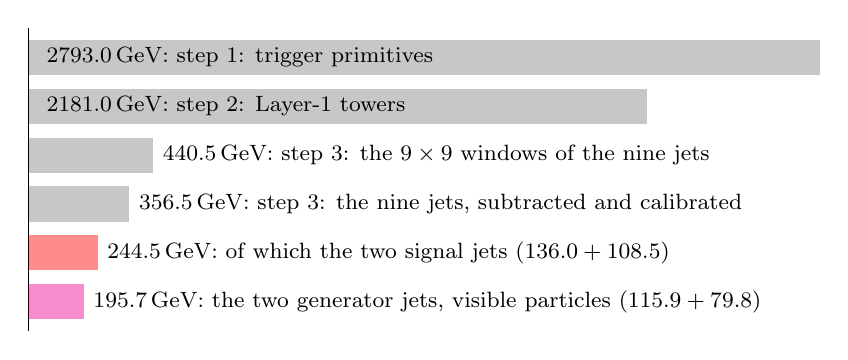
\begin{tikzpicture}[x=0.0036cm, y=0.62cm, font=\footnotesize]
\foreach \y/\v/\c/\t in {5/2793.0/black!22/{step 1: trigger primitives},
                         4/2181.0/black!22/{step 2: Layer-1 towers}}
{ \fill[\c] (0,\y-0.36) rectangle (\v,\y+0.36); \node[anchor=west] at (30,\y) {\v\,GeV: \t}; }
\foreach \y/\v/\c/\t in {3/440.5/black!22/{step 3: the $9\times9$ windows of the nine jets},
                         2/356.5/black!22/{step 3: the nine jets, subtracted and calibrated},
                         1/244.5/red!45/{of which the two signal jets ($136.0+108.5$)},
                         0/195.7/magenta!45/{the two generator jets, visible particles ($115.9+79.8$)}}
{ \fill[\c] (0,\y-0.36) rectangle (\v,\y+0.36); \node[anchor=west] at (\v,\y) {\v\,GeV: \t}; }
\draw (0,-0.6) -- (0,5.6);
\end{tikzpicture}
\caption{The energy part of the ledger as a picture: the transverse energy the trigger holds at each step
(table~\ref{tab:12_ledger}), down to the two jets it is looking for.}
\label{fig:12_funnel}
\end{figure}

Figure~\ref{fig:12_objects} is the display of the event at the end of the chapter: all that is left of it for the
global trigger. Compare it with figure~\ref{fig:11_mixed}, the $544\,407$ digis of the same event: the two magenta
circles are again the only thing the two pictures share, and now each has a red square in it.

\begin{figure}[!htb]
\centering
\includegraphics[width=0.93\textwidth]{12_L1T/out/l1t_12_L1T_global_objects_run1_event1.png}
\caption{The event as the global trigger receives it: 9 jets, 12 e/$\gamma$, 12 $\tau$, 1 muon and the sums
(\code{l1t\_12\_L1T\_global\_objects\_run1\_event1.png}). Red squares: jets with their $E_{\mathrm T}$ in GeV; blue
triangles: $\tau$ candidates; green dots: e/$\gamma$ candidates; star: the muon; the ticks on the left edge: the
direction of the missing transverse energy with HF (orange) and of the missing $H_{\mathrm T}$ (violet). Magenta
circles: the two generator jets.}
\label{fig:12_objects}
\end{figure}

\FloatBarrier
\section{Open problems for Phase-2}

The Phase-2 Level-1 trigger is a different machine: it has the tracker (tracks above $2\GeV$ at 40\,MHz), a
particle-flow reconstruction and PUPPI in firmware (the \emph{correlator}), the HGCAL in the endcaps, a latency of
$12.5\,\mu$s and an output rate of 750\,kHz. What follows is what the release, CMSSW\_15\_0\_5 with the era
\code{Phase2C17I13M9}, says about its state.

\textbf{The Run-3 trigger of this chapter still runs in Phase-2, on Run-3 primitives.} In
\path{L1Trigger/Configuration/python/SimL1Emulator_cff.py} the Phase-2 emulation is built as
\code{\_phase2\_siml1emulator = SimL1EmulatorTask.copy()} (line 62) and substituted under \code{phase2\_trigger} (line
279): a copy of the task of this chapter with modules added. Layer-1, Layer-2, the three track finders, the
$\mu$GMT and the $\mu$GT of Run~3 are all still executed on the Phase-2 detector; no modifier removes them
(\path{L1Trigger/L1TCalorimeter/python/simDigis_cff.py}, \path{L1Trigger/L1TMuon/python/simDigis_cff.py}, where
\code{phase2\_trigger} lists \code{simBmtfDigis}, \code{simEmtfDigis}, \code{simGmtStage2Digis} explicitly). The header
of the file says of the forward calorimeter: ``At the moment, there is no emulator available for upgrade HF Trigger
Primitives, so these missing (required!) inputs are presently ignored by downstream modules.'' The HCAL
trigger-primitive emulator of chapter~\ref{ch:11_DIGI} has no Phase-2 modifier at all
(\path{SimCalorimetry/HcalTrigPrimProducers/python/hcaltpdigi_cfi.py}: the last modifiers are \code{run3\_HB} and
\code{run3\_common}), and the Phase-2 calorimeter-trigger modules read \code{simHcalTriggerPrimitiveDigis}, the
collection of step~1 of this chapter. The Phase-2 ECAL barrel primitive (one per crystal, the reason for the new
barrel electronics) exists as \code{simEcalEBTriggerPrimitivePhase2Digis} but is switched on only by
\code{phase2\_ecalTP\_devel} (\path{SimCalorimetry/Configuration/python/ecalDigiSequence_cff.py}), a modifier that no era
includes; the era uses \code{simEcalEBTriggerPrimitiveDigis}, made from the Run-3 digitisation that
chapter~\ref{ch:11_DIGI} found in the same state.

\textbf{The pileup subtraction of the Phase-2 calorimeter towers was fitted in 2019.} The module that plays the
role of our Layer-1 (\path{l1tTowerCalibrationProducer_cfi.py} in \path{L1Trigger/L1CaloTrigger/python/}) opens with
``Choosen settings 6 March 2019, 10\_3\_X MTD samples''; its pileup estimate counts the towers hit, converts the count
to a number of vertices and the number of vertices to an energy per tower with ``Parameters derived on 6 March
2019 on 10\_3\_X MTD samples''. The 2024 calorimeter-jet emulator (\path{l1tPhase2CaloJetEmulator_cfi.py}) carries the
same numbers without the comment, under jet calibrations ``derived 26 June 2024 on 14\_0\_0\_pre3 131X QCD sample''.
This chapter showed for PU 60 what such an estimate is worth when the detector is not uniform (a jet's own energy
in its rings; tower ring 28, whose response changed by a factor of three between two global tags): scaled linearly
to PU 200 the towers of step~2 would hold some $7\TeV$, and the estimate that decides how much of it is a jet is a
fit on 2019 samples.

\textbf{A sum that is always zero.} Line 115 of \path{SimL1Emulator_cff.py} configures the Phase-2 calorimeter
$H_{\mathrm T}$ with \code{BXVCaloJetsInputTag = ("L1CaloJet", "CaloJets")}. No module has the label \code{L1CaloJet}:
the producer of line 108 is \code{l1tCaloJet}, and the collection it writes is called
\code{L1CaloJetCollectionBXV} (\path{L1Trigger/L1CaloTrigger/plugins/L1CaloJetProducer.cc}, line 341). In
the producer of the sum, \path{L1CaloJetHTTProducer.cc} of the same directory, the value is set to 0 and filled
only \code{if (bxvCaloJetsHandle.isValid())}:
the product is written, with the value 0, for every event. Nothing fails because nothing reads it: the Phase-2
global trigger takes no calorimeter jet at all (below).

\textbf{The Phase-2 jets are particle-flow jets, with corrections of March 2022 and cuts ``to be tuned''.} The jets
the Phase-2 global trigger receives are \code{l1tSC4PFL1PuppiCorrectedEmulator}, a seeded cone of radius 0.4 on
PUPPI candidates (\path{L1Trigger/Phase2L1GT/python/l1tGTProducer_cff.py}); the calorimeter jets above are not an
input. Their energy correction is \path{L1Trigger/Phase2L1ParticleFlow/data/jecs/jecs_20220308.root}
(\path{l1pfJetMet_cff.py}), and the cone of radius 0.8 uses the same file with the same directory,
\code{L1PuppiSC4EmuJets}: the wide jets are corrected as narrow ones. The hadron calibrations of the candidates
under them are tagged with the 11\_0\_X release (\code{hadcorr\_barrel\_110X.root}, \code{hfcorr\_110X.root},
\code{hadcorr\_HGCal3D\_TC\_110X.root}). The PUPPI parameters of \path{l1ctLayer1_cff.py} are annotated ``ballpark pT
from PU'' and ``ballpark alpha from PU''; in the HF, where our $\bar b$ jet is and where there are no tracks to
tell the pileup, a candidate needs $10\GeV$ (\code{ptCut}), the sort keeps ten per region (``to be tuned'') and
four buffer sizes are ``to be defined''. The vertex against which all of this is done is the single best one of a
histogram of track $z$ (\code{Algorithm = fastHisto}, \code{FH\_NVtx = 1},
\path{L1Trigger/VertexFinder/python/l1tVertexProducer_cfi.py}), with a comment that the track-\pt{} saturation
differs between the Technical Design Report and the firmware.

\textbf{The HGCAL trigger primitives are calibrated for an older HGCAL.} The era includes the modifiers
\code{phase2\_hgcalV10}, \code{V11} and \code{V16} together, and the trigger takes its settings from the first two:
\path{L1Trigger/L1THGCal/python/l1tHGCalBackEndLayer1Producer_cfi.py} switches the layer calibration off with ``we
still don't have layer calibrations for $>=$V9 geometry'', the trigger geometry class is
\code{HGCalTriggerGeometryV9Imp3}, and the e/$\gamma$ identification in use (\code{v10\_3151}) was ``trained using
TPG software version 3.15.1''.

\textbf{The Phase-2 menu is ``the first prototype menu''.} The Phase-2 global trigger is a separate
\code{cmsDriver} step (\code{L1P2GT}) whose default menu is \code{step1\_2024}
(\path{Configuration/Applications/python/ConfigBuilder.py}, line 1597;
\path{L1Trigger/Configuration/python/Phase2GTMenus/step1_2024.py} begins with the comment quoted). It has 40
algorithms against the 465 of this chapter. The jet ones are \code{pSinglePuppiJet230},
\code{pDoublePuppiJet112\_112}, \code{pPuppiHT450}, \code{pPuppiMHT140}, \code{pPuppiMET200} and a four-jet one; the
numbers are offline thresholds, translated to trigger thresholds with linear ``scalings'' (for jets in the barrel
an offset of $17.33\GeV$ and a slope of 1.28) that ``correspond to version v44 derived with the Annual Review 2024
config in the 14\_2\_x release'', one release series behind this one. There is no single-jet algorithm below
$230\GeV$, no prescaled ladder like \code{SingleJet35/60/90/120}, and the file named for $b$ tagging holds only
multi-muon seeds: an event like ours, two $b$ jets of $115\GeV$, has no hadronic way into the Phase-2 menu as it
stands, and the jet triggers on which jet calibration relies are not written yet.

\textbf{The Run-3 emulation itself is not uniform in time.} The simulated 2025 trigger of this chapter is
assembled from payloads of different years: the calorimeter parameters \code{2024\_v0\_1} (the release has
\code{v0\_3} and two 2025 versions in python), with, in the python of that version, jet compression tables
\code{2017v1} and the jet calibration \code{lut\_calib\_2023v0\_ECALZS\_PhiRing}; seven of the nineteen ECAL
trigger-primitive payloads \code{2018\_mc}; the HCAL ones \code{2019} and \code{2024}; the barrel muon parameters
\code{Stage2v1\_2018\_mc}; the menu of 2025 on the scales \code{scales\_2024\_05\_15}; and in the EMTF the era
\code{Run3\_2021} selects \code{PtAssignmentEngine2017} with the comment ``TODO - implement ver 2021''
(\path{L1Trigger/L1TMuonEndCap/src/EMTFSetup.cc}). The CSC shower thresholds of 2025 that \code{run3\_CSC\_2025} sets
are never used: the modifier writes \code{showerParams}, the producer reads \code{showerParam}
(\path{L1Trigger/CSCTriggerPrimitives/src/CSCBaseboard.cc}). The prescales are absent. Whoever compares a simulated
trigger efficiency with data should know which of the six steps were simulated as of 2025.

% chapter_13_HLT.tex -- chapter 13 of the JitJet book: the High Level Trigger, the second checkpoint (Rule G of the
% Constitution: B1, B2, one section per step, B4, B5). ONE sample: the event with its pileup (Rule H).
% Every number comes from test/13_HLT/out/ (ledger_13_HLT.txt, hlt_13_HLT.log, menu_13_HLT.txt, step5_HLT_13_HLT.log,
% the PNG pages); the companion doc/chapter/chapter_13_HLT.md lists them.

\chapter{13 -- HLT: the High Level Trigger reconstructs the event and keeps it}
\label{ch:13_HLT}

\section{What this chapter is about}

The Level-1 trigger of chapter~\ref{ch:12_L1T} said yes. In the detector that answer travels back to every readout
board, which sends its piece of the event to the data acquisition; an \emph{event builder} assembles the pieces, and
the complete event, about two megabytes of raw data, is handed to one computer of the \emph{High Level Trigger}
(HLT) farm. The HLT is the second and last checkpoint of the journey. Unlike the Level-1 trigger it is software: the
same CMSSW as the offline reconstruction, in faster versions, running on commercial computers with graphics cards. It
receives up to about $100\,000$ events per second from the Level-1 trigger and keeps a per cent or so of them: those
are the events that are written to disk and that an analysis will ever see.

The program of the HLT is the \emph{menu}, a list of \emph{paths}. A path is a sequence of modules: producers that
reconstruct something (hits, tracks, jets) and filters that cut on it. A path stops at the first filter that fails;
the event is kept if at least one path runs to its end. Every path starts with the question of chapter~\ref{ch:12_L1T},
``did my Level-1 seed fire?'', so that the farm reconstructs only what the Level-1 decision justifies, and modules
shared by many paths run once per event. The menu of this chapter, the 2025 menu of CMSSW\_15\_0\_5, has 898
paths. Its \emph{path of the book} is \code{HLT\_PFJet110}, the jet path that the seed \code{L1\_SingleJet90} of
chapter~\ref{ch:12_L1T} opens (figure~\ref{fig:13_path}). We follow it in five steps:

\begin{enumerate}
\item \textbf{the raw event, the Level-1 seed and the prescale}: the event as bytes; the Level-1 record unpacked; the
seed and prescale modules that open or close each path;
\item \textbf{calorimeter jets}: the ECAL and HCAL energies reconstructed, summed into towers, clustered into jets of
radius 0.4, corrected; a first, cheap cut on them;
\item \textbf{tracking and vertices}: the charged particles reconstructed from the pixel and strip hits, and the
collision points along the beam;
\item \textbf{particle flow and PF jets}: tracks and calorimeter clusters combined into a list of particles, and the
jets made of them, corrected;
\item \textbf{the decision of the paths}: the last filters, which of the 898 paths accept the event, and where it is
written: the datasets and the streams.
\end{enumerate}

\begin{figure}[!htb]
\centering
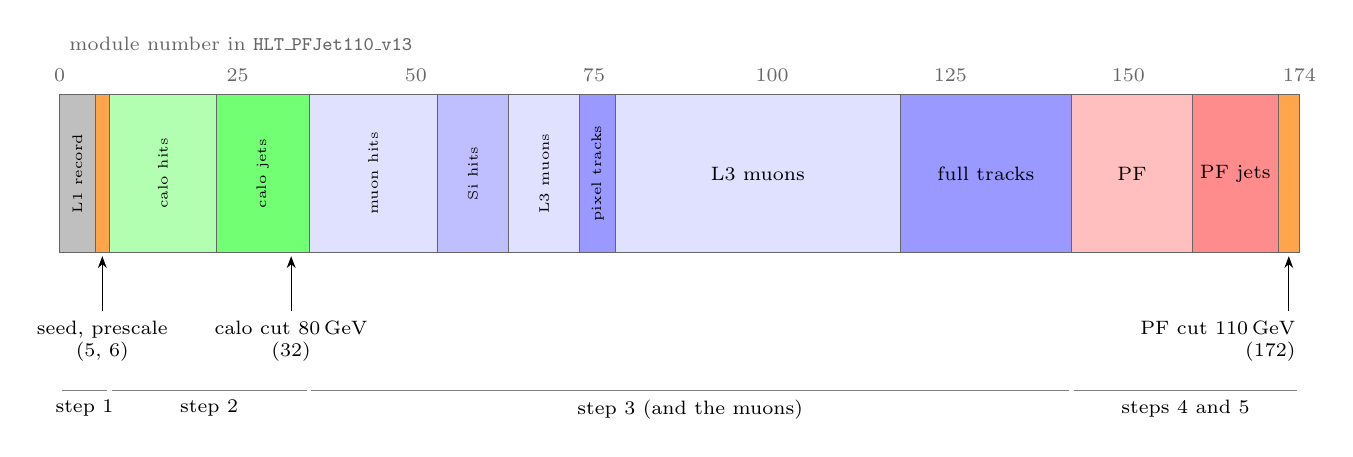
\begin{tikzpicture}[x=0.0905cm, y=1cm, font=\scriptsize]
% the 174 modules of HLT_PFJet110 in the order they run, as a bar (one unit = one module)
\foreach \a/\b/\c in {0/5/black!25, 5/7/orange!70, 7/22/green!30, 22/35/green!55, 35/53/blue!12, 53/63/blue!25,
  63/73/blue!12, 73/78/blue!40, 78/118/blue!12, 118/142/blue!40, 142/159/red!25, 159/171/red!45, 171/174/orange!70}
{ \fill[\c, draw=black!60, line width=0.3pt] (\a,0) rectangle (\b,2.0); }
\foreach \x/\t in {2.5/{L1 record}, 14.5/{calo hits}, 28.5/{calo jets}, 44/{muon hits}, 58/{Si hits}, 68/{L3 muons},
  75.5/{pixel tracks}}
{ \node[rotate=90, font=\tiny] at (\x,1.0) {\t}; }
\foreach \x/\t in {98/{L3 muons}, 130/{full tracks}, 150.5/{PF}, 165/{PF jets}}
{ \node at (\x,1.0) {\t}; }
\draw[->, >={Stealth[length=1.5mm]}] (6,-0.75) node[below, align=center] {seed, prescale\\(5, 6)} -- (6,-0.05);
\draw[->, >={Stealth[length=1.5mm]}] (32.5,-0.75) node[below, align=center] {calo cut $80\GeV$\\(32)} -- (32.5,-0.05);
\draw[->, >={Stealth[length=1.5mm]}] (172.5,-0.75) node[below left=0pt and -6pt, align=right] {PF cut $110\GeV$\\(172)} -- (172.5,-0.05);
\foreach \x in {0,25,50,75,100,125,150,174} \node[text=black!60] at (\x,2.25) {\x};
\node[anchor=west, text=black!60] at (0,2.65) {module number in \code{HLT\_PFJet110\_v13}};
\foreach \a/\b/\t in {0/7/{step 1}, 7/35/{step 2}, 35/142/{step 3 (and the muons)}, 142/174/{steps 4 and 5}}
{ \draw[black!50] (\a+0.3,-1.75) -- (\b-0.3,-1.75); \node[below] at ({(\a+\b)/2},-1.75) {\t}; }
\end{tikzpicture}
\caption{The path of the book, \code{HLT\_PFJet110}, module by module (\code{menu\_13\_HLT.txt}, section 2): 174
modules, of which the seed and the prescale are numbers 5 and 6, the cut on the calorimeter jets number 32 and the
cut on the PF jets number 172. Light blue: the reconstruction of the muons, which particle flow needs (68 modules).
Most of the path is shared with other paths and runs once per event.}
\label{fig:13_path}
\end{figure}

\begin{table}[!htb]
\centering\small\setlength{\tabcolsep}{4pt}
\caption{The five steps at a glance, for our event (\code{ledger\_13\_HLT.txt}).}
\label{tab:13_glance}
\begin{tabular}{@{}c>{\raggedright\arraybackslash}p{4.6cm}>{\raggedright\arraybackslash}p{4.2cm}>{\raggedright\arraybackslash}p{5.3cm}@{}}
\toprule
step & modules (examples) & what it makes & in our event \\
\midrule
1 & \code{hltGtStage2Digis}, \code{hltL1sSingleJet90}, \code{hltPrePFJet110} & the Level-1 record; for each path: go or stop & 1\,906\,128 bytes from 678 boards; 652 of 754 paths stop at their seed \\
2 & \code{hltTowerMakerForAll}, \code{hltAK4CaloJetsCorrected} & 2051 towers, calo jets & 2 jets above $30\GeV$: $118.5$ and $93.3\GeV$ \\
3 & \code{hltPixelTracks}, \code{hltMergedTracks}, \code{hltVerticesPF} & pixel tracks, full tracks, vertices & 2981 pixel tracks, 116 full tracks, 1 vertex: the signal \\
4 & \code{hltParticleFlow}, \code{hltAK4PFJetsCorrected} & 1366 particles, PF jets & 2 jets above $30\GeV$: $126.7$ and $86.7\GeV$ \\
5 & \code{hltSinglePFJet110}, \code{TriggerResults} & the decision of every path & 40 paths accept; \code{HLT\_PFJet110} by $16.7\GeV$ \\
\bottomrule
\end{tabular}
\end{table}

One event is followed (\path{test/13_HLT/run_13_HLT.sh}), the same as in chapter~\ref{ch:12_L1T}: the signal with
the 71, 68 and 54 collisions of bunch crossings $-1$, 0 and $+1$ (Rule H). Who made an object is read from the truth
the file still carries: the two generator jets of chapter~\ref{ch:07_GenJet}, the simulated position of every
collision along the beam (\code{addPileupInfo}, \code{genParticles:xyz0}).

\section{From the previous chapter}

One file of chapter~\ref{ch:12_L1T} enters (Rule E), \path{test/12_L1T/out/step4_L1_12_L1T.root}: the digis of
chapter~\ref{ch:11_DIGI} and the products of the Level-1 emulator, $12.3\,$MB. The decision it carries: 63 of the 465
Level-1 algorithms fired, among them \code{L1\_SingleJet90}, by $46\GeV$ on the $\bar b$ jet in the HF ($136.0\GeV$)
and by $18.5\GeV$ on the $b$ jet ($108.5\GeV$). That algorithm is the seed of \code{HLT\_PFJet110}: the door
through which the event enters this chapter.

The HLT does not read digis. It reads what the detector sends: \emph{raw data}, one block of bytes per readout board
(a FED, ``front-end driver''). The first part of the job of this chapter (\code{cmsDriver.py -s DIGI2RAW,HLT:@relval2025})
therefore packs the digis and the Level-1 record into raw data, as the readout would (\code{DIGI2RAW},
table~\ref{tab:13_packers}); the HLT then unpacks them again. Packing is not a copy: each packer writes the format of
its board, with headers, trailers and the zero suppression of the hardware, and the size of each block is what the
readout links have to carry. In production the Level-1 emulation and \code{DIGI2RAW} run in the same job, and three products
of the Level-1 job that the packers read were not kept by chapter~\ref{ch:12_L1T}; they are remade, with the same
configuration, at the head of the job (the companion, section~1). Nothing is added to the event: the digis are those
of chapter~\ref{ch:11_DIGI}, the Level-1 decision is that of chapter~\ref{ch:12_L1T}.

\begin{table}[!htb]
\centering\small
\caption{From the previous chapter: the packers of \code{DIGI2RAW}, the reverse of the unpackers that open every HLT
path (\code{step5\_HLT\_13\_HLT\_cfg.py}, the path \code{digi2raw\_step}, whose first three modules, not listed, are the
Level-1 products remade at the head of the job).}
\label{tab:13_packers}
\begin{tabular}{@{}>{\raggedright\arraybackslash}p{5.3cm}>{\raggedright\arraybackslash}p{4.2cm}>{\raggedright\arraybackslash}p{5.9cm}@{}}
\toprule
module & C++ type & packs \\
\midrule
\code{siPixelRawData}, \code{SiStripDigiToRaw} & \code{SiPixelDigiToRaw}, \ldots & the pixel and strip digis of chapter~\ref{ch:11_DIGI} \\
\code{ecalPacker}, \code{esDigiToRaw} & \code{EcalDigiToRaw}, \code{ESDigiToRaw} & ECAL data frames, selective-readout flags, ECAL trigger primitives; preshower \\
\code{hcalRawDatauHTR} & \code{HcalDigiToRawuHTR} & HB, HE, HF data frames and the HCAL trigger primitives \\
\code{cscpacker}, \code{dtpacker}, \code{rpcpacker}, \code{gemPacker} & & the muon digis and the CSC trigger primitives \\
\code{caloLayer1RawFed1354}, \code{1356}, \code{1358} & \code{L1TDigiToRaw} & the inputs and towers of calorimeter Layer-1 \\
\code{caloStage2Raw}, \code{bmtfStage2Raw}, \code{omtfStage2Raw}, \code{gmtStage2Raw} & & Layer-2 objects, track-finder candidates, $\mu$GMT muons \\
\code{gtStage2Raw} & \code{L1TDigiToRaw} & the record of the global trigger: the 512 bits and the objects (FED 1404) \\
\code{rawDataCollector} & \code{RawDataCollectorByLabel} & all of it, one \code{FEDRawDataCollection} \\
\bottomrule
\end{tabular}
\end{table}

Which menu? The one the release gives the 2025 simulation: \code{HLT:@relval2025} is \code{2025v10}
(\path{Configuration/HLT/python/autoHLT.py}), the frozen menu \code{/frozen/2025/2e34/v1.0/HLT/V2} of the 2025 data
taking (\path{HLTrigger/Configuration/python/HLT_2025v10_cff.py}), module for module the physics menu \code{GRun} of
the release. Its seeds name algorithms of the 2025 Level-1 menu of chapter~\ref{ch:12_L1T}, and every one exists:
\path{python/hltL1Menu_cff.py}, which checks the seeds against that menu, changes nothing, and the 898 paths run. (The
2024 version of this chapter ran the same menu on the 2024 Level-1 menu: 30 of the algorithms its seeds name did not
exist, and 37 paths had to be removed. The release has no 2024 HLT menu: \code{HLT:@relval2024} is a ``fake'' menu
of three paths.) The output adds to the input what the HLT made: $20.8\,$MB in all.

\section{Step 1: the raw event, the Level-1 seed and the prescale}

\textbf{What the step does.} The event arrives as 678 blocks of bytes, one per readout board that has data
(table~\ref{tab:13_raw}). More than half of it is the strip tracker, which has almost ten million channels; the calorimeters
are a fifth. Every path then starts with the same five modules (\code{HLTBeginSequence}): \code{hltTriggerType}
(is this a physics event?), \code{hltGtStage2Digis}, which unpacks the record of the Level-1 global trigger from its
board (FED 1404), \code{hltGtStage2ObjectMap}, which runs the global-trigger algorithm of chapter~\ref{ch:12_L1T}
once more on the unpacked objects to know \emph{which} objects satisfied each algorithm,
\code{hltOnlineMetaDataDigis} and \code{hltOnlineBeamSpot}, the position of the beam. Then come the two modules that decide whether the path runs at all.

\emph{The seed} (\code{HLTL1TSeed}, 224 of them in the menu) holds a logical expression of Level-1 algorithm names,
\code{L1SeedsLogicalExpression}; for \code{HLT\_PFJet110} it is \code{"L1\_SingleJet90"}. It reads the final
decision bit of each algorithm and evaluates the expression; if it is false the path stops there. If it is true the
seed also records the Level-1 objects that made the algorithm fire, so that a later module can look only where
the Level-1 trigger saw something (the electron and muon paths reconstruct in such \emph{regions}; the jet paths
reconstruct everywhere).

\emph{The prescaler} (\code{HLTPrescaler}, one per path, 893 in the menu) keeps one event in $N$ of those that reach
it. A path whose rate would be too high is not removed but prescaled: \code{HLT\_PFJet40} would fire on a large
fraction of all collisions, so in data taking it keeps only a small, known fraction of them, enough to measure the
jet trigger efficiency, while a path with a threshold high enough to fit in the bandwidth runs with $N=1$. The
values of $N$ are a table with one column per luminosity, loaded online by the \code{PrescaleService}.

\begin{plainwords}[The simulation runs without prescales, again]
The menu of the release is a \code{\_cff} file: the paths without the services of the online configuration. It has
no \code{PrescaleService} (\path{menu_13_HLT.txt}: ``no PrescaleService: every HLTPrescaler has prescale 1''), so,
as in chapter~\ref{ch:12_L1T}, every path runs unprescaled. In our event 0 of the 754 \code{HLT\_} and \code{DST\_}
paths is stopped by a prescaler. The question to ask of a simulated event is ``which paths accept it'', and then, for
the analysis one has in mind, whether those paths ran unprescaled in the data.
\end{plainwords}

\begin{plainwords}[How long it takes]
In this job, on one core of a processor without a graphics card, the HLT took about a minute to start (reading the
configuration of 4783 modules and the conditions of the global tag) and about six seconds for our event
(\path{step5_HLT_13_HLT.log}: from ``Begin processing'' at 13:23:46 to the closing of the input at 13:23:52), the first
event of the job, which also pays the initialisation of many modules. On the farm a process runs for days, the start
is paid once, the modules marked \code{@alpaka} run on the graphics cards, and the menu is designed so that the
average event takes a small fraction of a second. Our event is not average: it passes a jet seed, so the full
tracking and particle flow run.
\end{plainwords}

\textbf{The numbers of the event.} The record unpacked by the HLT is that of chapter~\ref{ch:12_L1T}, bit for bit:
63 algorithms fired, 9 jets, 12 e/$\gamma$, 12 $\tau$, one muon (figure~\ref{fig:13_seed}). Of the 754 physics
(\code{HLT\_}) and scouting (\code{DST\_}) paths, 652 stop at their seed: they cost the farm nothing but the
evaluation of an expression. 102 start their reconstruction. \code{hltL1sSingleJet90} is true and hands two Level-1
jets to the rest of its path, $136.0\GeV$ at $(\eta,\phi)=(-3.74,1.00)$ and $108.5\GeV$ at $(-1.52,-1.98)$: the two
jets of the signal. The seed of \code{HLT\_PFJet200}, \code{L1\_SingleJet120}, hands only the first; the seeds of the
paths above $200\GeV$ (\code{L1\_SingleJet180} and the like) are false.

\begin{table}[!htb]
\centering\small
\caption{Step 1: the raw event as the HLT receives it, by subsystem (\code{ledger\_13\_HLT.txt}, section 1; FED
numbers of \code{DataFormats/FEDRawData/interface/FEDNumbering.h}).}
\label{tab:13_raw}
\begin{tabular}{l rrr}
\toprule
subsystem & readout boards (FEDs) & kB & share \\
\midrule
strip tracker & 381 & 997.5 & 53.6\,\% \\
pixel tracker & 108 & 306.7 & 16.5\,\% \\
HCAL (HB, HE, HF, HO) & 44 & 240.6 & 12.9\,\% \\
ECAL preshower & 40 & 137.4 & 7.4\,\% \\
ECAL & 54 & 103.9 & 5.6\,\% \\
CSC & 36 & 46.9 & 2.5\,\% \\
Level-1 trigger & 7 & 27.1 & 1.5\,\% \\
GEM, DT, RPC & 8 & 1.3 & 0.1\,\% \\
\midrule
all & 678 & 1861.5 & \\
\bottomrule
\end{tabular}
\end{table}

\begin{figure}[!htb]
\centering
\includegraphics[width=0.93\textwidth]{13_HLT/out/hlt_13_HLT_seed_seed_run1_event1.png}
\caption{Step 1, what the HLT knows when a path starts: the Level-1 objects it unpacks
(\code{hlt\_13\_HLT\_seed\_seed\_run1\_event1.png}; squares: jets with their $E_{\mathrm T}$ in GeV, triangles: $\tau$,
dots: e/$\gamma$, star: the muon). The orange circles are the two jets that \code{hltL1sSingleJet90} records as the
reason it fired; magenta, the generator jets. The right panel: the raw data and the fate of the 754 paths.}
\label{fig:13_seed}
\end{figure}

\textbf{A path in the python of the menu.} The menu is a python file of $87\,551$ lines; our path is one of them,
and its first and last filters are two module definitions (\path{HLT_2025v10_cff.py}, shortened):

\begin{lstlisting}[style=py]
fragment.HLT_PFJet110_v13 = cms.Path( fragment.HLTBeginSequence + fragment.hltL1sSingleJet90
    + fragment.hltPrePFJet110 + fragment.HLTAK4CaloJetsSequence + fragment.hltSingleAK4CaloJet80
    + fragment.HLTAK4PFJetsSequence + fragment.hltPFJetsCorrectedMatchedToCaloJets80
    + fragment.hltSinglePFJet110 + fragment.HLTEndSequence )
fragment.hltL1sSingleJet90 = cms.EDFilter( "HLTL1TSeed",
    L1SeedsLogicalExpression = cms.string( "L1_SingleJet90" ), saveTags = cms.bool( True ), ... )
fragment.hltSinglePFJet110 = cms.EDFilter( "HLT1PFJet",
    inputTag = cms.InputTag( "hltPFJetsCorrectedMatchedToCaloJets80" ),
    MinPt = cms.double( 110.0 ), MaxEta = cms.double( 5.0 ), MinN = cms.int32( 1 ), ... )
\end{lstlisting}

\noindent The sequences (\code{HLTAK4CaloJetsSequence}, \code{HLTAK4PFJetsSequence}) expand into the modules of
figure~\ref{fig:13_path}: 209 entries, of which 174 distinct modules, since a sequence used twice brings modules that
have already run. The version suffix \code{\_v13} changes whenever the path changes; an analysis asks for
\code{HLT\_PFJet110\_v*}.

\textbf{What the seeds open.} The 102 paths that start are the ones the Level-1 decision of chapter~\ref{ch:12_L1T}
justifies, and they show what the HLT is for (table~\ref{tab:13_started}). Chapter~\ref{ch:12_L1T} found that 33 of
the 63 Level-1 algorithms needed an object the hard collision did not make: missing-energy seeds fired by an ETMHF
twice the neutrino, muon seeds fired by a pileup kaon, low-threshold jet and e/$\gamma$ seeds fired by the pileup of
the barrel. Those seeds open 30 missing-energy paths and 13 muon paths here. The HLT stops 29 of the 30
missing-energy paths, most of them at the first cut on the missing $H_{\mathrm T}$ of the calo jets
(\code{HLTMhtFilter}), and 12 of the 13 muon paths, which want a muon above 8, 10, 12 or $23\GeV$ (or two above
$50\GeV$). (With the 2024
settings the ring-28 jets of chapter~\ref{ch:12_L1T} had also opened 13 VBF and 6 multijet paths, all stopped here.) Reconstructing the event better than the Level-1 trigger could
is how the HLT brings the rate down by a factor of a hundred.

\begin{table}[!htb]
\centering\small
\caption{Step 1 and step 5: the 102 \code{HLT\_} and \code{DST\_} paths whose seed fired, by kind, and the filter types
that stopped them (\code{ledger\_13\_HLT.txt}, section 5).}
\label{tab:13_started}
\begin{tabular}{@{}l rr >{\raggedright\arraybackslash}p{7.2cm}@{}}
\toprule
kind of path & accepted & stopped & stopped by (C++ type of the filter) \\
\midrule
single jets, dijets & 16 & 14 & \code{HLT1PFJet} 4, \code{HLT1CaloJet} 4, \code{HLTDiPFJetAveEtaFilter} 4, \code{HLTDiCaloJetAveFilter} 2 \\
multijets, VBF, electrons & 0 & 0 & seeds not fired (2024: 6, 13 and 2 paths started, all stopped) \\
missing energy, $H_{\mathrm T}$ & 1 & 29 & \code{HLTMhtFilter} 16, \code{HLT1PFMET} 5, \code{HLTDeDxFilter} 3, \code{HLTHtMhtFilter} 2, others 3 \\
muons & 1 & 12 & \code{HLTMuonL2FromL1TPreFilter} 9, \code{HLTMuonL3PreFilter} 3 \\
scouting & 7 & 0 & \\
no object, L1 seed only, calibration & 15 & 0 & \\
isolated tracks, PPS, monitoring & 0 & 7 & \code{TriggerResultsFilter} 3, \code{HLTPixelIsolTrackL1TFilter} 2, \code{HLTPPSCalFilter} 2 \\
\midrule
all & 40 & 62 & \\
\bottomrule
\end{tabular}
\end{table}

\FloatBarrier
\section{Step 2: calorimeter jets}

\textbf{What the step does.} The paths that need jets first reconstruct the calorimeters, in four stages
(figure~\ref{fig:13_path}, modules 7 to 32).

\emph{Rec-hits.} The ECAL and HCAL boards are unpacked into digis, and a rec-hit is made of each digi: one energy and
one time per crystal or HCAL cell. The ECAL fits the ten samples of a crystal with a sum of pulse templates (the
``multifit''); the HCAL barrel and endcap do the same with eight samples (``MAHI''); the HF, whose signal is shorter
than 25\,ns, takes the charge of the one sample of the bunch crossing. These modules are written for graphics cards (their C++ type ends in
\code{@alpaka}); on a computer without one, as here, the same code runs on the processor.

\emph{Towers.} \code{hltTowerMakerForAll} (\code{CaloTowersCreator}) sums the rec-hits of each $\eta$--$\phi$ cell
into a tower, the same grid as the trigger towers of chapter~\ref{ch:12_L1T} (the towers 28 and 29 of the endcap are
separate here, and from $|i\eta|=21$ on a tower is $10^\circ$ wide). Only rec-hits above a threshold enter
(table~\ref{tab:13_towercuts}); the HO, the tail catcher outside the solenoid, is given the weight $10^{-99}$, that is
none.

\emph{Jets.} \code{hltAK4CaloJets} clusters the towers with the anti-$k_{\mathrm T}$ algorithm of radius 0.4, the
algorithm of the generator jets of chapter~\ref{ch:07_GenJet}, on every tower above $0.3\GeV$.
\code{hltAK4CaloJetsIDPassed} drops jets that look like noise (fewer than 2 rec-hits carrying 90\,\% of the energy).

\emph{Corrections.} A calorimeter jet measures less than the particles that made it, and pileup adds to it. The
jet energy corrections of the HLT, the payload \code{AK4CaloHLT} of the global tag
(\code{JetCorrectorParametersCollection\_Run3Winter24Digi\_AK4CaloHLT}), are applied in levels. \emph{L1FastJet}
subtracts the pileup: the energy density $\rho$, the median of $E_{\mathrm T}/\text{area}$ over a grid of
$0.55\times0.55$ cells of the whole event (\code{hltFixedGridRhoFastjetAllCalo}), times the area of the jet, with a
parametrised dependence on $\eta$ and \pt. \emph{L2Relative} makes the response flat in $\eta$ and \pt{} (the factor
that a simulated jet needs, on average, to come back to its generator jet). \emph{L3Absolute} and
\emph{L2L3Residual} are 1 in simulation (formula ``1'' in the payload). Each level is a formula of \pt, $\rho$ and the
area, with parameters in bins of $\eta$ (82 bins).

\begin{table}[!htb]
\centering\small
\caption{Step 2: the thresholds of the towers (\code{hltTowerMakerForAll}, \code{menu\_13\_HLT.txt}, section 3), in GeV.}
\label{tab:13_towercuts}
\begin{tabular}{@{}l>{\raggedright\arraybackslash}p{9.6cm}@{}}
\toprule
ECAL barrel & a crystal above 0.07; the ECAL sum of a tower above 0.2 \\
ECAL endcap & a crystal above 0.3; the ECAL sum of a tower above 0.45 \\
HCAL barrel & a cell above its threshold in the payload \code{HcalPFCuts\_2025\_mc} (\code{usePFThresholdsFromDB = True}); the python values 0.4 (depth 1), 0.3 are not used \\
HCAL endcap & the same payload; the python values 0.1 (depth 1), 0.2 are not used \\
HF & a long fibre above 0.5, a short fibre above 0.85 \\
HO & weight $10^{-99}$: not used \\
\bottomrule
\end{tabular}
\end{table}

\textbf{The numbers of the event.} The calorimeters give $11\,193$ rec-hits with $3198.9\GeV$ of transverse energy,
half of it in the HF ($1606.2\GeV$; table~\ref{tab:13_rechits}). The HF has the fewest cells and the most energy: its
1728 rec-hits hold $50.8\TeV$ of energy, the forward pileup at small angle, which is little transverse energy each.
The barrel ECAL has 956 rec-hits, half as many as with the 2024 settings: the higher zero suppression of
chapter~\ref{ch:11_DIGI}. The rec-hits make 2051 towers with $2842.9\GeV$ (barrel 342.8, endcap 882.9, HF
$1617.2\GeV$), close to the $2793\GeV$ of trigger primitives of chapter~\ref{ch:12_L1T}. The energy density is
$\rho=36.3\GeV$ per unit area: a jet of radius 0.4, area 0.50, collects $18\GeV$ of pileup on average. And so the
clustering finds 190 jets, 23 of them above $30\GeV$ before the corrections (figure~\ref{fig:13_calo}). After them,
two are left above $30\GeV$, and they are the two jets of the signal (table~\ref{tab:13_calojets}).

\begin{table}[!htb]
\centering\small
\caption{Step 2: the calorimeter rec-hits and towers of the event (\code{hlt\_13\_HLT.log}, lines \code{rechits} and
\code{towers}; $E_{\mathrm T}$ from the cell positions of the geometry).}
\label{tab:13_rechits}
\begin{tabular}{l rrrr c l rr}
\toprule
rec-hits & $n$ & $\sum E$ & $\sum E_{\mathrm T}$ & max $E_{\mathrm T}$ & & towers & $n$ & $\sum E_{\mathrm T}$ \\
\cmidrule(lr){1-5}\cmidrule(lr){7-9}
ECAL barrel & 956 & 208.3 & 142.6 & 3.01 & & barrel & 492 & 342.8 \\
ECAL endcap & 2515 & 2135.3 & 378.7 & 5.07 & & endcap & 771 & 882.9 \\
HCAL barrel & 2162 & 671.3 & 493.4 & 7.81 & & HF & 788 & 1617.2 \\
HCAL endcap & 3832 & 3028.3 & 578.0 & 9.63 & & all & 2051 & 2842.9 \\
HF & 1728 & 50\,809.4 & 1606.2 & 61.15 & & \quad EM / HAD & & 1090.3 / 1752.6 \\
\bottomrule
\end{tabular}
\end{table}

\begin{table}[!htb]
\centering\small
\caption{Step 2: the two signal jets as AK4 calo jets, level by level (\code{hlt\_13\_HLT.log}, lines \code{CaloJet};
the factors are recomputed from the payload and agree with \code{hltAK4CaloJetsCorrected}). A jet of the pileup for
comparison.}
\label{tab:13_calojets}
\begin{tabular}{@{}l rrr@{}}
\toprule
 & $b$ jet & $\bar b$ jet (HF) & a pileup jet \\
\midrule
generator jet \pt{} (visible) & 117.8 (79.8) & 115.9 & -- \\
calo jet $\eta$, $\phi$ & $-1.58$, $-2.08$ & $-3.72$, $0.96$ & $3.66$, $-0.36$ \\
towers, EM fraction & 33, 0.56 & 17, 0.27 & 16, 0.35 \\
raw \pt{} & 70.9 & 163.5 & 39.5 \\
after L1FastJet & 57.4 ($\times0.809$) & 119.9 ($\times0.734$) & 10.3 ($\times0.260$) \\
after L2Relative & \textbf{93.3} ($\times1.627$) & \textbf{118.5} ($\times0.987$) & \textbf{12.5} ($\times1.218$) \\
Level-1 jet of chapter~\ref{ch:12_L1T} & 108.5 & 136.0 & -- \\
\bottomrule
\end{tabular}
\end{table}

\emph{The $b$ jet} has $70.9\GeV$ of towers for $79.8\GeV$ of visible particles, pileup included: the calorimeter
response to hadrons is well below one. The pileup subtraction takes $13.5\GeV$ and the relative correction multiplies
by 1.63, to $93.3\GeV$. \emph{The $\bar b$ jet} in the HF has the opposite problem: $163.5\GeV$ of towers for a jet of
$115.9\GeV$, pileup and the HF response together; the subtraction takes $43.6\GeV$ (the area, the $\rho$ and the
parameters of this $\eta$ bin), and the relative correction is close to one. The pileup jets lose three quarters of
their energy to L1FastJet: what they are made of is exactly the $\rho$ that is subtracted.

The cut of the step is a single line of the menu: \code{hltSingleAK4CaloJet80}, at least one corrected calo jet
with $\pt\geq80\GeV$ and $\abseta<5$. Both signal jets pass. It costs a few milliseconds and protects what follows:
a path whose calo jets are too soft stops here, before the tracking.

\begin{figure}[!htb]
\centering
\includegraphics[width=0.93\textwidth]{13_HLT/out/hlt_13_HLT_calo_towers_run1_event1.png}
\caption{Step 2, the calorimeter towers of the event with the corrected AK4 calo jets above $20\GeV$ (red dashed
circles, \pt{} in GeV) and the generator jets (magenta) (\code{hlt\_13\_HLT\_calo\_towers\_run1\_event1.png}). The
grid is that of the trigger towers of chapter~\ref{ch:12_L1T}; a tower of $10^\circ$ or $20^\circ$ is shared over the
$5^\circ$ cells it covers. The bright bands at $\abseta\approx2.7$--3 and the HF are the pileup.}
\label{fig:13_calo}
\end{figure}

\begin{figure}[!htb]
\centering
\includegraphics[width=0.49\textwidth,trim=0 0 475 0,clip]{13_HLT/out/hlt_13_HLT_calo_jet1_run1_event1.png}\hfill
\includegraphics[width=0.49\textwidth,trim=0 0 475 0,clip]{13_HLT/out/hlt_13_HLT_calo_jet2_run1_event1.png}
\caption{Step 2, the towers around the two signal jets, $E_{\mathrm T}$ in GeV (\code{hlt\_13\_HLT\_calo\_jet1/jet2\_run1\_event1.png}).
Left: the $b$ jet; right: the $\bar b$ jet in the HF. The red dashed square is the $9\times9$ window of the
Level-1 jet of chapter~\ref{ch:12_L1T} nearest to the calo jet (for the $b$ jet centred on its seed,
$(i\eta,i\phi)=(-18,50)$, one tower away in both from the calo jet at $(-19,49)$; for the $\bar b$ jet both at
$(-34,12)$): in the same window the HLT towers hold $77.7\GeV$ for the $b$ jet (Layer-1: $74.5\GeV$) and
$215.9\GeV$ for the $\bar b$ jet (Layer-1: $189.0\GeV$).}
\label{fig:13_calozoom}
\end{figure}

\FloatBarrier
\section{Step 3: tracking and vertices}

\textbf{What the step does.} Tracking is the most expensive part of the HLT, and the menu does it in a careful order
(figure~\ref{fig:13_path}, modules 53 to 141).

\emph{Pixel tracks.} The pixel hits are clustered and given a position (\code{hltSiPixelClusters},
\code{hltSiPixelRecHits}); a \emph{cellular automaton} (\code{hltPixelTracksSoA}) links hits of three or four pixel
layers into short tracks, above $0.9\GeV$, with a helix fit. Pixel tracks are fast, but four points give a modest
momentum resolution.

\emph{Pixel vertices.} The pixel tracks above $0.5\GeV$ are clustered in $z$ into vertices (\code{hltPixelVertices}),
which are ordered by the sum of $\pt^2$ of their tracks: the first one is the \emph{primary vertex}, assumed to be
the interesting collision. \code{hltTrimmedPixelVertices} then keeps only the vertices whose sum of $\pt^2$ is at least
30\,\% of the first one (\code{fractionSumPt2 = 0.3}).

\emph{Full tracks.} Iteration 0 (\code{hltIter0PFLowPixelSeedsFromPixelTracks}) takes as seeds the pixel tracks that
point to a trimmed vertex (within $0.3\cm$ in $z$ and $0.1\cm$ in $r$), extends them through the ten layers of the
strip tracker with \code{mkFit} (a vectorised pattern recognition), fits them again and keeps the high-purity ones. A
second iteration, the \emph{doublet recovery}, seeds with pairs of pixel hits that iteration 0 did not use, for the
tracks that crossed only two pixel layers. The two are merged (\code{hltMergedTracks}), and the vertices of particle
flow are fitted from them (\code{hltVerticesPF}, deterministic annealing in $z$ and an adaptive fit).

\begin{plainwords}[Why the HLT reconstructs one collision of 69]
A bunch crossing of our event holds 69 collisions. Full tracking of all of them would take most of the time budget
of the farm. The HLT therefore reconstructs everything cheaply with pixels, decides which collision is the
interesting one (the vertex with the largest $\sum\pt^2$, because a hard scattering makes harder tracks than a
pileup collision) and builds full tracks only from the pixel tracks that come from it, and from vertices almost as
hard. In our event the trimming keeps one vertex out of 31, and it is the signal. The pileup collisions remain pixel
tracks, except those within the $3\mm$ seeding window around it. This works when the hard collision has hard charged particles in the tracker; an event whose jets are both
outside the tracker would have its primary vertex chosen among the pileup.
\end{plainwords}

\textbf{The numbers of the event.} The tracker gives $20\,925$ pixel clusters and $115\,249$ strip clusters. The
cellular automaton makes 2981 pixel tracks, of which 156 above $10\GeV$; they form 31 pixel vertices, for the 68
in-time pileup collisions and the signal. The first pixel vertex is at $z=3.107\cm$, with 40 pixel tracks: the signal,
whose simulated vertex is at $z=3.112\cm$ (no pileup collision is within a millimetre of it). It is the only vertex
the trimming keeps. Iteration 0 builds 108 tracks, the doublet recovery 8 more: 116 full tracks, 49 of them above
$1\GeV$, with on average 4.0 pixel and 9.3 strip hits. They make one PF vertex, at $z=3.111\cm$, $7\um$ from the
simulated one (the pixel vertex was $53\um$ away), with 107 tracks; 61 tracks with $121.8\GeV$ are within a millimetre of it
(figure~\ref{fig:13_track}). Another 27 are within a millimetre of pixel vertex 8, a pileup collision $2.2\mm$ away,
inside the $3\mm$ window of iteration 0.

\begin{table}[!htb]
\centering\small
\caption{Step 3: the tracking of the HLT, stage by stage, for our event (\code{hlt\_13\_HLT.log}, lines \code{clusters},
\code{tracks}, \code{vertices}; the cuts from \code{menu\_13\_HLT.txt}, section 3).}
\label{tab:13_tracking}
\begin{tabular}{@{}>{\raggedright\arraybackslash}p{4.9cm}>{\raggedright\arraybackslash}p{6.6cm} r@{}}
\toprule
stage (module) & what it does, with which cuts & our event \\
\midrule
pixel and strip clusters & neighbouring channels above threshold & 20\,925 / 115\,249 \\
pixel tracks (\code{hltPixelTracks}) & cellular automaton, 3 or 4 pixel hits, $\pt>0.9\GeV$ & 2981 \\
pixel vertices (\code{hltPixelVertices}) & clusters in $z$ of pixel tracks above $0.5\GeV$ & 31 \\
kept vertices (\code{hltTrimmedPixelVertices}) & $\sum\pt^2\geq0.3\times$ the first vertex & 1 \\
iteration 0 & seeds: pixel tracks within $0.3\cm$ in $z$ of a kept vertex; \code{mkFit}; high purity & 108 \\
doublet recovery & seeds: pixel pairs in regions of inactive pixel modules & 8 \\
merged (\code{hltMergedTracks}) & the two, without duplicates & 116 \\
PF vertices (\code{hltVerticesPF}) & deterministic annealing in $z$, adaptive fit & 1 \\
\bottomrule
\end{tabular}
\end{table}

\emph{The pileup vertices.} Each pixel vertex can be compared with the simulated collisions (table~\ref{tab:13_vertices}):
the first ten are each within $80\um$ of a simulated collision, most within $40\um$. The HLT knows where the pileup
collisions are; it only does not build their full tracks. Only the first vertex is kept: no other pixel vertex reaches 30\,\% of its
$\sum\pt^2$.

\begin{table}[!htb]
\centering\small
\caption{Step 3: the first ten pixel vertices, in the order of the HLT, and the simulated collision nearest to each in
$z$ (\code{hlt\_13\_HLT.log}, lines \code{vertex pixel}; ``pu$k$'' is the $k$-th in-time pileup collision of
\code{addPileupInfo}).}
\label{tab:13_vertices}
\begin{tabular}{r rrl r}
\toprule
& $z$ [cm] & pixel tracks & nearest simulated collision & $\Delta z$ [$\mu$m] \\
\midrule
0 & 3.1066 & 40 & the signal & 53 \\
1 & $-0.3305$ & 22 & pu9 & 79 \\
2 & $-5.4560$ & 31 & pu30 & 17 \\
3 & 2.0815 & 22 & pu42 & 12 \\
4 & 0.3620 & 27 & pu35 & 16 \\
5 & $-2.0472$ & 13 & pu51 & 3 \\
6 & $-2.8665$ & 18 & pu29 & 9 \\
7 & 2.4981 & 25 & pu22 & 34 \\
8 & 2.8856 & 20 & pu34 & 64 \\
9 & 1.4886 & 28 & pu10 & 39 \\
\bottomrule
\end{tabular}
\end{table}

\emph{The two jets.} Inside the $b$ jet ($\Delta R<0.4$) there are 7 tracks with $50.1\GeV$, six of them from the
signal vertex; the charged particles of the generator jet have $32.6\GeV$. Two tracks more than with the 2024
settings: the electron of the $B^-$ decay ($5.0\GeV$) and a track of $11.2\GeV$ a hair ($\Delta R=0.04$) from the
pion of $11.0\GeV$, with no simulated particle of its own: a duplicate, or a secondary; which is not established. The $\bar b$ jet, at $\eta=-3.75$, is
outside the tracker ($\abseta<2.5$): its $44.0\GeV$ of charged particles leave no track. For the HLT this jet will be
calorimeter only, in step~4 as in step~2.

\begin{figure}[!htb]
\centering
\includegraphics[width=0.49\textwidth,trim=0 0 475 0,clip]{13_HLT/out/hlt_13_HLT_track_etaphi_run1_event1.png}\hfill
\includegraphics[width=0.49\textwidth,trim=0 0 475 0,clip]{13_HLT/out/hlt_13_HLT_track_vertices_run1_event1.png}
\caption{Step 3 (\code{hlt\_13\_HLT\_track\_etaphi/vertices\_run1\_event1.png}). Left: the 116 full tracks in
$\eta$--$\phi$; black, the 61 within $1\mm$ in $z$ of the signal vertex; grey, the others (size $\propto\log(1+\pt)$).
The blue dashed lines are the end of the tracker; the $\bar b$ jet (magenta, left) has no track. Right: along the
beam, the 31 pixel vertices (circles, height = pixel tracks; full: the one kept by the trimming), the one PF vertex
(bar) and, below the axis, the simulated in-time collisions (blue) and the signal (star).}
\label{fig:13_track}
\end{figure}

\FloatBarrier
\section{Step 4: particle flow and PF jets}

\textbf{What the step does.} Particle flow (PF) describes the event as a list of particles, using for each the
detector that measures it best: the tracker for charged hadrons, the ECAL for photons, the calorimeters for neutral
hadrons (figure~\ref{fig:13_path}, modules 142 to 170). The rec-hits of step 2 are clustered again, with the PF
algorithms (\code{hltParticleFlowClusterECALUnseeded}, \code{HCAL}, \code{HF}, preshower). \code{hltParticleFlowBlock}
links the elements that belong together: a track to the ECAL and HCAL clusters it points to, an ECAL cluster to the
HCAL cluster behind it. Its elements are of four kinds only: tracks, ECAL, HCAL and HF clusters. There are no
electron tracks (the GSF tracks of the offline reconstruction), so the HLT particle flow makes no electron: the
electron of the $B^-$ decay of chapter~\ref{ch:06_Decay} becomes a charged hadron or a photon. \code{hltParticleFlow}
turns each block into particles: a charged hadron per track, with the energy of the track; a photon or a neutral
hadron for the calorimeter energy that the tracks do not explain; in the HF, which has no tracker in front, an ``HF
hadronic'' or ``HF electromagnetic'' particle per cluster.

The particles are clustered into AK4 jets (\code{hltAK4PFJets}), all of them: the HLT jets of this menu do not remove
the charged particles of the pileup vertices. The pileup is subtracted as for the calo jets, with a $\rho$ made of
the PF candidates (\code{hltFixedGridRhoFastjetAll}) and the payload \code{AK4PFHLT}
(\code{JetCorrectorParametersCollection\_Run3Winter24Digi\_AK4PFHLT}). Its parameters are binned in $\eta$
\emph{and} $\phi$: 118 bins, because a patch of the barrel on the negative side ($-1.566<\eta<0$,
$-1.2<\phi<-0.8$) has its own; our jets are not in it.

\textbf{The numbers of the event.} 1366 particles with $\sum\pt=2655.8\GeV$ (table~\ref{tab:13_pf},
figure~\ref{fig:13_pf}). More than half of them, 783, are in the HF; within the tracker, 110 of the 515 particles are
charged. The energy density is $\rho=36.7\GeV$ per unit area. The 192 PF jets include 13 above $30\GeV$ before the
corrections and 2 after: the two signal jets again.

\begin{table}[!htb]
\centering\small
\caption{Step 4: the PF candidates of the event (\code{hlt\_13\_HLT.log}, lines \code{pfcands}).}
\label{tab:13_pf}
\begin{tabular}{l rr c l rr}
\toprule
kind & $n$ & $\sum\pt$ [GeV] & & region & $n$ & charged \\
\cmidrule(lr){1-3}\cmidrule(lr){5-7}
charged hadron & 117 & 181.9 & & tracker, $\abseta<2.5$ & 515 & 110 \\
photon & 238 & 196.3 & & $2.5<\abseta<3$ & 68 & 8 \\
neutral hadron & 209 & 702.5 & & HF, $\abseta>3$ & 783 & 0 \\
HF hadronic & 700 & 1486.0 & & & & \\
HF electromagnetic & 101 & 86.0 & & & & \\
muon & 1 & 3.0 & & & & \\
electron & 0 & 0 & & & & \\
\midrule
all & 1366 & 2655.8 & & all & 1366 & 118 \\
\bottomrule
\end{tabular}
\end{table}

\emph{The $b$ jet} is 29 particles: 7 charged hadrons with $50.1\GeV$, 20 photons with $28.4\GeV$, 2 neutral hadrons
with $5.8\GeV$; $83.7\GeV$ raw, against $70.9\GeV$ for the calo jet, because the charged hadrons now have the energy
of their tracks. L1FastJet subtracts $11.0\GeV$ ($\times0.869$), L2Relative multiplies by 1.192: $\mathbf{86.7\GeV}$.
That is 9\,\% above the $79.8\GeV$ of visible particles of chapter~\ref{ch:07_GenJet}, the $11\GeV$ of the extra
track of step~3 (with the 2024 settings, without it, the PF jet had $80.3\GeV$); the $37.5\GeV$ of the
neutrino are lost to every trigger. \emph{The $\bar b$ jet} is 17 HF hadronic particles, $156.8\GeV$ raw; L1FastJet
takes $27.6\GeV$ ($\times0.824$) and L2Relative $\times0.981$: $\mathbf{126.7\GeV}$, 9\,\% above the generator jet.
Particle flow cannot help in the HF: the PF jet is a calorimeter jet with another clustering and other corrections.

\emph{The other jets.} Table~\ref{tab:13_pfjets} lists the corrected PF jets above $15\GeV$. After the two signal
jets come seven jets of 16 to $21\GeV$ with no generator jet behind them. Five are beyond the tracker and made only
of neutral energy (the HF hadronic fraction of the jet at $\eta=-4.22$ is 1.00): pileup that no track can tell
from a jet. The corrections push them down by factors of 0.4 to 0.6, the subtraction of $\rho$ doing most of it.

\begin{table}[!htb]
\centering\small
\caption{Step 4: the corrected AK4 PF jets above $15\GeV$, with their energy fractions (\code{hlt\_13\_HLT.log}, lines
\code{PFJet}; charged hadron, neutral hadron, photon, HF hadronic; the factor is the product of the levels).}
\label{tab:13_pfjets}
\begin{tabular}{rrrr rrrr r l}
\toprule
\pt{} & raw & $\eta$ & $\phi$ & ch. & neut. & phot. & HF had. & factor & generator jet \\
\midrule
126.7 & 156.8 & $-3.77$ & 0.96 & 0.00 & 1.00 & 0.00 & 1.00 & 0.808 & 115.9 ($\bar b$) \\
86.7 & 83.7 & $-1.58$ & $-2.08$ & 0.59 & 0.07 & 0.34 & 0.00 & 1.035 & 117.8 ($b$) \\
21.2 & 24.2 & 1.11 & 2.43 & 0.37 & 0.31 & 0.32 & 0.00 & 0.876 & -- \\
19.6 & 37.7 & 3.41 & 1.94 & 0.00 & 0.95 & 0.00 & 0.95 & 0.521 & -- \\
18.3 & 34.7 & 4.61 & $-1.23$ & 0.00 & 1.00 & 0.00 & 1.00 & 0.526 & -- \\
18.0 & 34.6 & $-4.22$ & 1.25 & 0.00 & 1.00 & 0.00 & 1.00 & 0.522 & -- \\
16.7 & 29.9 & 4.78 & 1.67 & 0.00 & 1.00 & 0.00 & 1.00 & 0.561 & -- \\
16.3 & 19.7 & 1.02 & 1.69 & 0.05 & 0.73 & 0.22 & 0.00 & 0.827 & -- \\
16.1 & 38.9 & 3.69 & $-0.36$ & 0.00 & 1.00 & 0.00 & 1.00 & 0.414 & -- \\
\bottomrule
\end{tabular}
\end{table}

\begin{figure}[!htb]
\centering
\includegraphics[width=0.93\textwidth]{13_HLT/out/hlt_13_HLT_pf_candidates_run1_event1.png}
\caption{Step 4, the 1366 PF candidates of the event by kind, with the corrected AK4 PF jets above $20\GeV$ (red dashed
circles) and the generator jets (\code{hlt\_13\_HLT\_pf\_candidates\_run1\_event1.png}). Black: charged hadrons; green:
photons; violet: neutral hadrons; orange and cyan: HF hadronic and electromagnetic. The HF is a regular grid: one
particle per cluster, and the clusters follow the towers.}
\label{fig:13_pf}
\end{figure}

\begin{figure}[!htb]
\centering
\includegraphics[width=0.49\textwidth,trim=0 0 475 0,clip]{13_HLT/out/hlt_13_HLT_pf_jet1_run1_event1.png}\hfill
\includegraphics[width=0.49\textwidth,trim=0 0 475 0,clip]{13_HLT/out/hlt_13_HLT_pf_jet2_run1_event1.png}
\caption{Step 4, the two signal jets particle by particle (\code{hlt\_13\_HLT\_pf\_jet1/jet2\_run1\_event1.png}; full
markers: the constituents of the PF jet, open: the other candidates, \pt{} in GeV for those above $4\GeV$). Left: the
$b$ jet, 29 constituents of three kinds; right: the $\bar b$ jet, 17 HF clusters, one of $86.9\GeV$.}
\label{fig:13_pfzoom}
\end{figure}

\FloatBarrier
\section{Step 5: the decision of the paths}

{\sloppy\textbf{What the step does.} At the end of each path a filter cuts on the objects the path built. For
\code{HLT\_PFJet110} there are two modules (figure~\ref{fig:13_path}, 171 and 172).
\code{hltPFJetsCorrectedMatchedToCaloJets80} keeps the corrected PF jets within $\Delta R<0.5$ of a calo jet that
passed the cut of step 2, so that a PF jet is never accepted alone where the calorimeter saw nothing; then
\code{hltSinglePFJet110} (\code{HLT1PFJet}) asks for one of them with $\pt\geq110\GeV$ and $\abseta<5$. The ladders
of the jet paths are built the same way, with a calo cut below the PF cut ($80\GeV$ for 110, 110 for 140, 170 for
200). A path that reaches its end
sets its bit in \code{TriggerResults}, and the filters with \code{saveTags} record their objects in
\code{hltTriggerSummaryAOD}, so that an analysis can later ask which jet fired the trigger.\par}

The event is then sorted. A \emph{dataset} is an OR of paths (\code{JetMET0} has 150, all the jet and missing-energy
paths); a \emph{stream} is an OR of datasets and is a file of the data acquisition. The menu has 99 datasets and 68
streams; each dataset is a path of its own (\code{Dataset\_JetMET0}: a \code{TriggerResultsFilter} on its paths). An
event can be in several datasets, and is then written several times.

\textbf{The numbers of the event.} \code{HLT\_PFJet110} accepts it (table~\ref{tab:13_jetpaths},
figure~\ref{fig:13_ladders}): the seed fired, two calo jets passed $80\GeV$, two PF jets are matched to them, and one
passes $110\GeV$: the $\bar b$ jet in the HF, $126.7\GeV$, by $16.7\GeV$. The $b$ jet alone, $86.7\GeV$, would not
have been enough. One step up the ladder the event stops: \code{HLT\_PFJet140} fails by $13.3\GeV$; so does
\code{HLT\_PFJetFwd140}, the forward version. \code{HLT\_AK8PFJet140}, the same with jets of radius 0.8, fails by
$0.9\GeV$: the AK8 jet around the $\bar b$ jet has $139.1\GeV$.

\begin{table}[!htb]
\centering\small
\caption{Step 5: the single-jet and dijet paths around our event, and the module that decided
(\code{hlt\_13\_HLT.log}, lines \code{path:} and \code{ladder}; values in GeV).}
\label{tab:13_jetpaths}
\begin{tabular}{@{}>{\raggedright\arraybackslash}p{4.1cm}>{\raggedright\arraybackslash}p{4.3cm}>{\raggedright\arraybackslash}p{3.5cm}>{\raggedright\arraybackslash}p{3.4cm}@{}}
\toprule
path & L1 seed & what the event has & decision \\
\midrule
\code{HLT\_PFJet40}, \code{60}, \code{80} & \code{L1\_ZeroBias} & PF jet 126.7 & accepted \\
\code{HLT\_PFJet110} & \code{L1\_SingleJet90} & calo jet 118.5, PF jet 126.7 & \textbf{accepted}, by 16.7 \\
\code{HLT\_PFJet140} & \code{L1\_SingleJet90} & calo 118.5 $\geq$ 110; PF 126.7 & stopped by the PF cut \\
\code{HLT\_PFJet200} & \code{L1\_SingleJet120} & calo jet 118.5 $<$ 170 & stopped by the calo cut \\
\code{HLT\_PFJet260} \ldots{} \code{550} & \code{L1\_SingleJet180} \ldots & & stopped by the seed \\
\code{HLT\_PFJetFwd80}, \code{140} & \code{L1\_SingleJet60\_FWD2p5}, \code{90\_FWD2p5} & PF jet 126.7 at $\abseta>2.7$ & 80 accepted, 140 stopped \\
\code{HLT\_AK8PFJet80}, \code{140} & \code{L1\_ZeroBias}, \code{L1\_SingleJet90} & AK8 PF jet 139.1 & 80 accepted, 140 stopped \\
\code{HLT\_DiPFJetAve80}, \code{140} & \code{L1\_ZeroBias}, \ldots & PF average 106.7, calo 105.9 & 80 accepted, 140 stopped by the calo cut \\
\code{HLT\_DiPFJetAve60} \ldots{} \code{160\_HFJEC} & \ldots & no jet with $\abseta<1.4$ & stopped \\
\code{HLT\_PFHT180} \ldots{} \code{1050} & \code{L1\_HTT}\ldots & & stopped by the seed \\
\bottomrule
\end{tabular}
\end{table}

\begin{plainwords}[A path made for this event, which misses it]
\code{HLT\_DiPFJetAve100\_HFJEC} exists to calibrate the HF with dijets: a \emph{tag} jet in the barrel,
$\abseta<1.4$, where the response is known, and a \emph{probe} jet in the HF, $2.7<\abseta<5.5$, back to back
($\Delta\phi>2.5$), with an average \pt{} above $100\GeV$ (\code{hltDiPFJetAve100ForHFJEC}). Our event is a dijet with
one jet in the HF and the other opposite in $\phi$ ($\Delta\phi=3.04$), average $106.7\GeV$. The filter finds the
probe, $126.7\GeV$ at $\eta=-3.77$, and no tag: the $b$ jet is at $\eta=-1.58$, $0.18$ beyond the barrel cut. The
four HF calibration paths whose seed fired (60, 80, 100, 160) fail on it; the other three (220, 260, 300) stop at
their seed.
\end{plainwords}

\begin{figure}[!htb]
\centering
\includegraphics[width=0.93\textwidth]{13_HLT/out/hlt_13_HLT_seed_ladders_run1_event1.png}
\caption{Step 5, the ladders of the jet paths (\code{hlt\_13\_HLT\_seed\_ladders\_run1\_event1.png}). One line per
family; the ticks are the thresholds in the path names, green if the path accepted the event, red if a filter stopped
it, grey if its Level-1 seed did; the blue triangle is the event (the leading PF jet, the leading jet with
$\abseta>2.7$, the leading AK8 jet, the average of the two leading jets, $H_{\mathrm T}$).}
\label{fig:13_ladders}
\end{figure}

\begin{figure}[!htb]
\centering
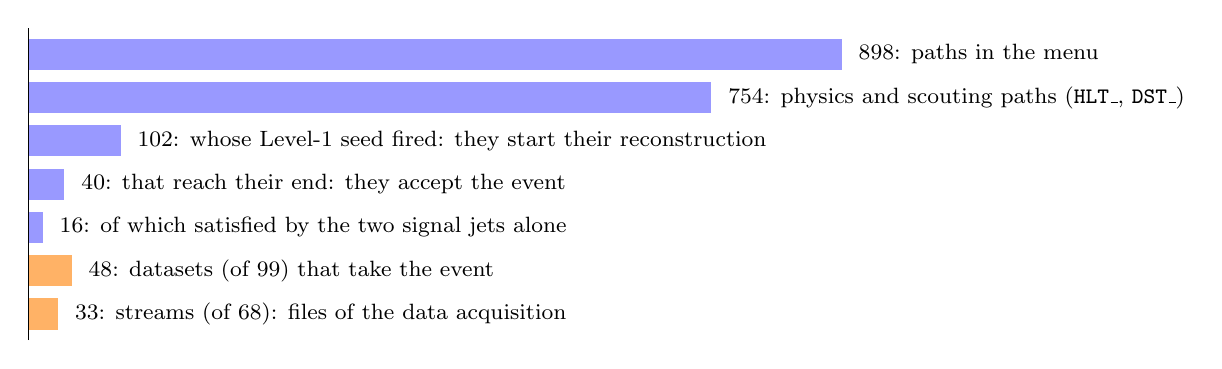
\begin{tikzpicture}[x=0.0115cm, y=0.55cm, font=\footnotesize]
\foreach \y/\v/\t in {6/898/{paths in the menu}, 5/754/{physics and scouting paths (\code{HLT\_}, \code{DST\_})},
  4/102/{whose Level-1 seed fired: they start their reconstruction}, 3/40/{that reach their end: they accept the event},
  2/16/{of which satisfied by the two signal jets alone}, 1/48/{datasets (of 99) that take the event},
  0/33/{streams (of 68): files of the data acquisition}}
{ \fill[\ifnum\y>1 blue!40\else orange!60\fi] (0,\y-0.36) rectangle (\v,\y+0.36);
  \node[anchor=west] at (\v+8,\y) {\v: \t}; }
\path (0,0) -- (940,0);
\draw (0,-0.6) -- (0,6.6);
\end{tikzpicture}
\caption{Step 5, the decision as a funnel (\code{ledger\_13\_HLT.txt}, section 5). The length of a bar is the number
of paths (blue) or of datasets and streams (orange).}
\label{fig:13_funnel}
\end{figure}

\textbf{The record of the decision.} What an analysis finds in the file about \code{HLT\_PFJet110}: its bit in
\code{TriggerResults}, and in \code{hltTriggerSummaryAOD} the objects of its three filters with \code{saveTags}, as
(\pt, $\eta$, $\phi$) (\path{hlt_13_HLT.log}, lines \code{filter:}):

\begin{lstlisting}[style=txt]
path: name=HLT_PFJet110_v13 accept=1 stage=accept seedFired=1 last=hltBoolEnd lastIndex=208 nModules=209
filter: label=hltL1sSingleJet90     type=HLTL1TSeed  n=2 | L1Jet(136.0,-3.74,1.00) L1Jet(108.5,-1.52,-1.98)
filter: label=hltSingleAK4CaloJet80 type=HLT1CaloJet n=2 | Jet(118.5,-3.72,0.96) Jet(93.3,-1.58,-2.08)
filter: label=hltSinglePFJet110     type=HLT1PFJet   n=1 | Jet(126.7,-3.77,0.96)
\end{lstlisting}

\noindent Each step of the path narrowed the list: two Level-1 jets, two calo jets, one PF jet. An analysis that uses
this trigger checks that its own jet is close to that last object, and measures the efficiency of the path with
events of a lower, prescaled path, \code{HLT\_PFJet80} for example, in which the jet above $110\GeV$ was not required.

\textbf{What else accepts it.} 40 of the 754 paths (table~\ref{tab:13_accepted}, figure~\ref{fig:13_funnel}). Sixteen are jet paths satisfied by
the two signal jets. Two need an object the hard collision did not make: \code{HLT\_Mu3\_PFJet40} finds the muon of
chapter~\ref{ch:12_L1T}, the kaon of a pileup collision that decayed in flight, now reconstructed by the HLT
(with $3.1\GeV$ by the muon chambers alone, \code{hltL2Muons}, then $3.0\GeV$ with the tracker,
\code{hltIterL3MuonCandidates}), and pairs it with the $b$ jet; \code{HLT\_CaloMET90\_NotCleaned} finds a missing
transverse energy of $138.5\GeV$ in the towers, where the neutrino carries $37.5\GeV$. Three paths ask only for their
Level-1 seed. Twelve select nothing at all: zero bias, random, ``physics'' (any event), calibration and monitoring
paths, which in data run prescaled or on special events. Seven are scouting paths (\code{DST\_}): they save not the
raw event but a compact list of HLT objects, at a high rate; four of them are seeded by the CICADA anomaly score of
chapter~\ref{ch:12_L1T}.

\begin{table}[!htb]
\centering\small
\caption{Step 5: the 40 \code{HLT\_} and \code{DST\_} paths that accept the event, by what satisfies them
(\code{ledger\_13\_HLT.txt}, section 5).}
\label{tab:13_accepted}
\begin{tabular}{@{}>{\raggedright\arraybackslash}p{4.1cm} c >{\raggedright\arraybackslash}p{9.6cm}@{}}
\toprule
satisfied by & paths & which \\
\midrule
the two signal jets & 16 & \code{HLT\_PFJet40}, \code{60}, \code{80}, \code{110}; \code{PFJetFwd40}, \code{60}, \code{80}; \code{AK8PFJet40}, \code{60}, \code{80}; \code{AK8PFJetFwd40}, \code{60}, \code{80}; \code{DiPFJetAve40}, \code{60}, \code{80} \\
a pileup object & 2 & \code{HLT\_Mu3\_PFJet40} (the muon of a pileup kaon), \code{HLT\_CaloMET90\_NotCleaned} ($138.5\GeV$) \\
the L1 seed alone & 3 & \code{HLT\_L1SingleMuCosmics}, \code{HLT\_L1ETMHadSeeds}, \code{HLT\_L1AlwaysTrue} \\
no object & 12 & \code{HLT\_ZeroBias} (and \code{\_Alignment}, \code{\_Beamspot}), \code{HLT\_Physics}, \code{HLT\_Random}, \code{HLT\_EphemeralPhysics}, \code{HLT\_EphemeralZeroBias}, \code{HLT\_EcalCalibration}, \code{HLT\_HcalCalibration}, \code{HLT\_HcalNZS}, \code{HLT\_HcalPhiSym}, \code{HLT\_PPSRandom} \\
scouting & 7 & \code{DST\_PFScouting\_CICADA*} (4), \code{DST\_PFScouting\_ZeroBias}, \code{DST\_ZeroBias}, \code{DST\_Physics} \\
\bottomrule
\end{tabular}
\end{table}

\textbf{Where the event goes.} 48 of the 99 datasets and 33 of the 68 streams accept it. For physics the ones that
matter are \code{JetMET0} and \code{JetMET1} (18 of their 150 paths fired; the two are copies that split the rate),
\code{Muon0} and \code{Muon1} (one path of 129, \code{HLT\_Mu3\_PFJet40}: the event would be in the muon dataset
because of a pileup kaon), \code{ZeroBias}, and the scouting dataset \code{ScoutingPFRun3}. The jet analysis this
book is heading to reads \code{JetMET}: the stream \code{PhysicsJetMET0}, the dataset \code{JetMET0}, the trigger bit
\code{HLT\_PFJet110\_v13} with the $\bar b$ jet as its object.

\FloatBarrier
\section{Ledger and display}

A checkpoint has a ledger in two parts. The first is what the HLT \emph{sees}, step by step
(table~\ref{tab:13_ledger}, top), with the two jets of the signal followed through every step
(figure~\ref{fig:13_twojets}); nothing of it is added to or removed from the recorded event, whose raw data are those
of step~1. The second is the decision (bottom).

\begin{table}[!htb]
\centering\small
\caption{The ledger of the High Level Trigger (\code{ledger\_13\_HLT.txt}). Top: what each step reconstructs.
Middle: the two jets of the signal. Bottom: the decision.}
\label{tab:13_ledger}
\begin{tabular}{@{}p{7.0cm} r >{\raggedright\arraybackslash}p{4.4cm}@{}}
\toprule
\multicolumn{3}{@{}l}{\emph{what the HLT sees}} \\
step 1: raw event (678 FEDs) & 1862 kB & strip tracker 54\,\% \\
step 1: Level-1 algorithms fired / jets unpacked & 63 / 9 & as in chapter~\ref{ch:12_L1T} \\
step 2: rec-hits, $\sum E_{\mathrm T}$ & 3198.9 GeV & 11\,193 rec-hits \\
step 2: towers, $\sum E_{\mathrm T}$ & 2842.9 GeV & 2051 towers; HF 1617.2 \\
step 2: $\rho$ (calorimeter) & 36.3 GeV & per unit area \\
step 2: calo jets above 30 GeV, raw / corrected & 23 / 2 & of 190 \\
step 3: pixel tracks / pixel vertices / kept & 2981 / 31 / 1 & 68 + 1 collisions \\
step 3: full tracks, $\sum\pt$ & 116, 179.5 GeV & of the signal vertex: 61, 121.8 \\
step 3: PF vertices & 1 & $7\um$ from the signal \\
step 4: PF candidates, $\sum\pt$ & 1366, 2655.8 GeV & HF: 783 \\
step 4: $\rho$ (particle flow) & 36.7 GeV & per unit area \\
step 4: PF jets above 30 GeV, raw / corrected & 13 / 2 & of 192 \\
\midrule
\multicolumn{3}{@{}l}{\emph{the two signal jets: $b$ ($\eta=-1.59$) and $\bar b$ ($\eta=-3.75$), \pt{} in GeV}} \\
generator jet (visible particles) & 117.8 (79.8) / 115.9 & chapter~\ref{ch:07_GenJet} \\
Level-1 jet & 108.5 / 136.0 & chapter~\ref{ch:12_L1T} \\
calo jet, raw $\rightarrow$ corrected & 70.9 $\rightarrow$ 93.3 / 163.5 $\rightarrow$ 118.5 & step 2 \\
tracks in the jet & 7, 50.1 / 0 & step 3 \\
PF jet, raw $\rightarrow$ corrected & 83.7 $\rightarrow$ 86.7 / 156.8 $\rightarrow$ 126.7 & step 4 \\
\midrule
\multicolumn{3}{@{}l}{\emph{decision}} \\
paths \code{HLT\_} and \code{DST\_} & 754 & \\
\quad stopped by the L1 seed / a prescale / a filter & 652 / 0 / 62 & \\
\quad accepting the event & 40 & 16 on the signal jets alone \\
\code{HLT\_PFJet110}, the path of the book & accepted & by 16.7 GeV, on the $\bar b$ jet \\
highest single-jet threshold passed & 110 & 140 failed by 13.3 GeV \\
datasets / streams & 48 / 33 & \code{JetMET0}, \code{PhysicsJetMET0} \\
\bottomrule
\end{tabular}
\end{table}

Read downwards, the ledger says what each step of the HLT is for. The calorimeters see $2843\GeV$ of towers; the
pileup subtraction leaves two jets, which are the signal. The tracker sees 2981 pixel tracks; the HLT builds its 116
full tracks around one collision, which is the signal. Particle flow brings the $b$ jet to $86.7\GeV$, near its visible energy, and
cannot help the $\bar b$ jet, which no tracker sees. The decision then turns on that jet: \code{HLT\_PFJet110} fires
because the HF jet is measured at $126.7\GeV$, 9\,\% above its true \pt. Of the 40 paths that accept the event, 16
are satisfied by the two signal jets alone, and the jet path of the book is one of them.

\paragraph{What the year changed.} With the 2024 settings (the first version of this chapter; the companion compares
the two step by step) the menu had to be cut to 861 paths, and 41 of 717 accepted the event. With 2025 the menu runs
whole and 40 of 754 accept: the VBF, multijet and electron paths do not even start, because their Level-1 seeds,
fired in 2024 by the ring-28 jets and a cluster of $8\GeV$, did not fire; one CICADA scouting path is lost with
\code{L1\_CICADA\_VTight}. The path of the book is untouched: the $\bar b$ jet moved from 125.9 to $126.7\GeV$ and
\code{HLT\_PFJet110} accepts by $16.7\GeV$ instead of $15.9\GeV$. Table~\ref{tab:13_years} puts the two side by side.

\begin{table}[!htb]
\centering\small
\caption{The same event through the HLT with the 2024 and the 2025 settings of the release (the 2024 numbers are
those of the first version of this chapter; companion, last section). Values in GeV unless stated.}
\label{tab:13_years}
\begin{tabular}{@{}l rr >{\raggedright\arraybackslash}p{5.6cm}@{}}
\toprule
 & 2024 & 2025 & why \\
\midrule
HLT menu, paths run & 861 & 898 & 2024: 37 removed, their seeds not in the Level-1 menu \\
Level-1 algorithms fired / L1 jets & 57 / 12 & 63 / 9 & no jet in tower ring 28 (chapter~\ref{ch:12_L1T}) \\
raw event, kB (ECAL) & 1929 (173) & 1862 (104) & ECAL barrel zero suppression (chapter~\ref{ch:11_DIGI}) \\
ECAL barrel rec-hits & 2039 & 956 & the same \\
towers, $\sum E_{\mathrm T}$ & 3085.5 & 2842.9 & the two ECAL changes of chapter~\ref{ch:11_DIGI} \\
$\rho$ calorimeter / particle flow & 40.0 / 36.4 & 36.3 / 36.7 & \\
calo jets $b$ / $\bar b$, corrected & 88.5 / 113.4 & 93.3 / 118.5 & \\
full tracks / pixel vertices & 115 / 27 & 116 / 31 & pixel digis and templates of 2025 \\
PF jets $b$ / $\bar b$, corrected & 80.3 / 125.9 & 86.7 / 126.7 & $b$: one track of $11\GeV$ more \\
paths started / accepted & 124 / 41 & 102 / 40 & VBF, multijet, electron seeds not fired \\
\code{HLT\_PFJet110}, margin & 15.9 & 16.7 & \\
datasets / streams & 47 / 32 & 48 / 33 & \\
\bottomrule
\end{tabular}
\end{table}

\begin{figure}[!htb]
\centering
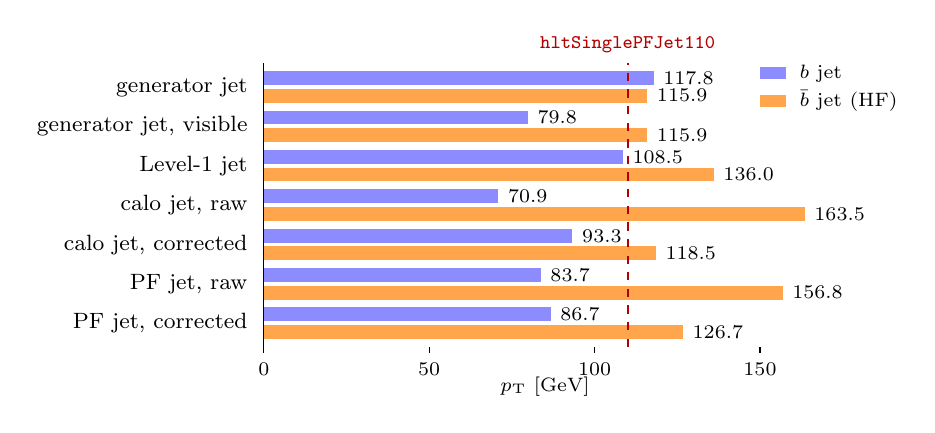
\begin{tikzpicture}[x=0.042cm, y=0.5cm, font=\footnotesize]
\foreach \y/\t/\b/\bb in {6/{generator jet}/117.8/115.9, 5/{generator jet, visible}/79.8/115.9, 4/{Level-1 jet}/108.5/136.0,
                          3/{calo jet, raw}/70.9/163.5, 2/{calo jet, corrected}/93.3/118.5, 1/{PF jet, raw}/83.7/156.8, 0/{PF jet, corrected}/86.7/126.7}
{ \node[anchor=east] at (-2,\y) {\t};
  \fill[blue!45] (0,\y+0.05) rectangle (\b,\y+0.4); \node[anchor=west, font=\scriptsize] at (\b,\y+0.22) {\b};
  \fill[orange!70] (0,\y-0.4) rectangle (\bb,\y-0.05); \node[anchor=west, font=\scriptsize] at (\bb,\y-0.22) {\bb}; }
\draw (0,-0.6) -- (0,6.6);
\draw[red!70!black, dashed, thick] (110,-0.6) -- (110,6.6) node[above, font=\scriptsize] {\code{hltSinglePFJet110}};
\foreach \x in {0,50,100,150} { \draw (\x,-0.6) -- (\x,-0.75) node[below, font=\scriptsize] {\x}; }
\node[font=\scriptsize] at (85,-1.6) {\pt{} [GeV]};
\fill[blue!45] (150,6.2) rectangle (158,6.5); \node[anchor=west, font=\scriptsize] at (159,6.35) {$b$ jet};
\fill[orange!70] (150,5.5) rectangle (158,5.8); \node[anchor=west, font=\scriptsize] at (159,5.65) {$\bar b$ jet (HF)};
\end{tikzpicture}
\caption{The two jets of the signal through the trigger (table~\ref{tab:13_ledger}, middle). The $b$ jet loses its
neutrino and never comes back above $110\GeV$; the $\bar b$ jet, in the HF, is measured above its true \pt{} at every
step and carries the decision.}
\label{fig:13_twojets}
\end{figure}

Figure~\ref{fig:13_objects} is the event as the HLT records it: the objects of the filters of the paths that
accepted it. Compare it with figure~\ref{fig:12_objects}, the 34 objects that the Level-1 trigger handed over, and
with figure~\ref{fig:11_mixed}, the $544\,407$ digis of the same event: what is left are the two jets the journey has
followed since chapter~\ref{ch:01_ME}.

\begin{figure}[!htb]
\centering
\includegraphics[width=0.93\textwidth]{13_HLT/out/hlt_13_HLT_seed_objects_run1_event1.png}
\caption{The event as the HLT records it (\code{hlt\_13\_HLT\_seed\_objects\_run1\_event1.png}): the objects of the last
filter of each accepted \code{HLT\_} path, from \code{hltTriggerSummaryAOD}. Red squares: AK4 PF jets ($126.7$ and
$86.7\GeV$); open orange squares: AK8 PF jets; the tick on the left edge: the direction of the calorimeter missing
transverse energy. Magenta circles: the two generator jets. The right panel lists the physics datasets.}
\label{fig:13_objects}
\end{figure}

\FloatBarrier
\section{Open problems for Phase-2}

The Phase-2 HLT will receive 750\,kHz from the Level-1 trigger instead of 100\,kHz, at a pileup of 140 to 200, with
a new tracker, the HGCAL in the endcaps and a timing layer (MTD). Its menu in the release is \code{75e33}
(\path{HLTrigger/Configuration/python/HLT_75e33_cff.py} and the directory \path{HLT_75e33/}; \code{HLT:@relvalRun4}
in \path{Configuration/HLT/python/autoHLT.py}). What follows compares it with the Run-3 menu of this chapter, step by
step; every statement is a line of the release or of the global tag of the Phase-2 workflows,
\code{150X\_mcRun4\_realistic\_v1} (\path{Configuration/AlCa/python/autoCond.py}, line 111).

\textbf{An event like ours has no Phase-2 path.} The schedule of \code{75e33} (line 353 of the \code{\_cff}) has 54
entries: 32 \code{HLT\_}, 16 \code{L1T\_} (Level-1 objects cut at offline-equivalent thresholds), 4 \code{MC\_}, the
final path and an endpath, against the 898 paths of the 2025 menu. Its jet and energy-sum paths are \code{HLT\_AK4PFPuppiJet520} (seed \code{pSinglePuppiJet230}),
\code{HLT\_PFPuppiHT1070}, \code{HLT\_PFPuppiMETTypeOne140\_PFPuppiMHT140}, two double-jet paths with two $b$ tags
(two jets above $128\GeV$ with $\abseta<2.4$ and $\Delta\eta<1.6$, \path{hltDoublePFPuppiJets128MaxEta2p4_cfi.py}) and
four four-jet paths with three $b$ tags. There is no ladder of prescaled single-jet paths like \code{HLT\_PFJet40}
\ldots{} \code{450}, no forward jet path, no dijet-average path and no HF calibration path like
\code{HLT\_DiPFJetAve100\_HFJEC}. The paths that the jet energy scale and the trigger efficiencies are measured with
in Run~3, the 16 that accepted our event among them, are not written yet; and a $b\bar b$ pair with a jet in the HF
fails even the $b$-tag paths, which require $\abseta<2.4$ for both jets.

\textbf{The pileup subtraction of the Phase-2 HLT jets is an identity.} The jets of the Phase-2 HLT are PUPPI jets,
corrected in three levels with the payload \code{AK4PFPuppiHLT} (\path{HLT_75e33/modules/hltAK4PFPuppiJetCorrectorL1_cfi.py}:
\code{L1FastjetCorrectorProducer}, $\rho$ from \code{hltFixedGridRhoFastjetAll}, made of all PF candidates). In the
global tag that payload is \code{JetCorrectorParametersCollection\_Phase2Spring23ticlv4\_MC\_AK4PFPuppiHLT\_v1}, one
interval of validity written on 21 September 2023, and in it the L1FastJet level and the L3Absolute level both have
the formula ``1'' (\code{conddb dump} of the payload): the menu computes $\rho$ and runs a corrector that multiplies by
one. PUPPI removes the pileup particle by particle, so no offset may be the intention, but then a jet's response
rests on L2Relative alone, which has 19 bins of $\eta$ from $-5.2$ to $5.2$ (the Run-3 payload of this chapter has
82 bins of $\eta$, and 118 cells of $\eta\times\phi$). The name says ``ticlv4''; the menu already carries the
\code{ticl\_v5} alternative of the HGCAL reconstruction (\path{HLT_75e33/sequences/HLTIterTICLSequence_cfi.py}). The
same global tag gives the Run-3 HLT labels \code{AK4PFHLT} and \code{AK4CaloHLT} as \code{Run3Summer21} payloads.

\textbf{The pileup estimate of PUPPI is a count of pixel clusters, and in the HF it has no tracks.}
\path{HLT_75e33/modules/hltPFPuppi_cfi.py} has three regions: $\abseta<2.5$, $2.5<\abseta<3.5$ and
$3.5<\abseta<10$. In the first two the neutral threshold grows with the pileup (\code{MinNeutralPt} 0.5105 and
$0.821\GeV$ plus a slope of $9.51\times10^{-6}$ and $1.902\times10^{-5}$), and the pileup is measured by the number of
pixel clusters (\code{PUProxyValue = hltPixelClustersMultiplicity}), not by vertices. In the last region,
\code{useCharged = False} and a neutral particle needs $3.656\GeV$. Our $\bar b$ jet is in that region: 17 HF
particles of which, at PU 200, PUPPI can only cut the soft ones. The file has no comment, no date and no reference to
the sample its numbers were fitted on. The HF calibration of particle flow is off in both menus
(\code{calibHF\_use = False}, \path{HLT_75e33/modules/hltParticleFlowTmpBarrel_cfi.py}, line 121, as in
\code{hltParticleFlow} of the 2025 menu), and the Phase-2 particle flow reads the hadron calibration with the empty label
(line 122), which in the Phase-2 global tag is \code{PFCalibration\_Run3\_mc\_offline}: an offline Run-3 calibration,
where the Run-3 HLT reads its own (\code{calibrationsLabel = "HLT"}, \code{PFCalibration\_Run3\_2024\_online\_v1} in our
global tag).

\textbf{The tracking reconstructs every collision, without the timing layer.} Step~3 showed that the Run-3 HLT keeps
one pixel vertex of 31 (\code{hltTrimmedPixelVertices}, \code{fractionSumPt2 = 0.3}) and builds full tracks only
around it. In Phase-2 the seeds of the first iteration are all the pixel tracks, with no vertex
(\path{HLT_75e33/modules/hltInitialStepSeeds_cfi.py}: \code{InputVertexCollection = ""}, \code{usePV = False}); the only
vertex trimmer of the menu is in a muon path. At PU 200 the full tracking of every collision is the price of not
choosing the hard one too early. The primary vertices are found in $z$ only: \code{DA\_vect}, \code{useTiming =
False} (\path{hltOfflinePrimaryVertices_cfi.py}, line 22), no track times, although the era includes the timing layer
(\code{phase2\_timing}, \code{phase2\_timing\_layer}). The timing was the argument for the MTD at 200 collisions per
crossing.

\textbf{No cheap cut before the expensive steps.} A Run-3 jet path cuts on calo jets (step~2) before it pays for the
tracking. The Phase-2 jet paths go from the Level-1 seed (\code{PathStatusFilter} on a Phase-2 global-trigger
algorithm) to the full reconstruction and cut only on the PUPPI jets
(\path{HLT_75e33/paths/HLT_AK4PFPuppiJet520_cfi.py}); the calo jets of the menu serve only the vertex sorting. With
750\,kHz of input, every seeded event pays for tracking, HGCAL clustering and PUPPI.

\textbf{What the menu itself says.} The comments of \code{75e33} are few, and they are about unfinished business:
``Removed temporarily until final decision on L1T tau Phase-2'' (line 411, the two tau paths),
``Run3 thresholds. Will be overwritten with valid aging customisation'' (the HCAL thresholds of the e/$\gamma$
$H/E$, \path{hltEgammaHoverEL1Seeded_cfi.py}), ``Probably need to move elsewhere in the final setup''
(\path{HLTInitialStepSequence_cfi.py}). And the Run-3 lesson of this chapter applies to Phase-2 as well: a menu works
only with the Level-1 menu it was written for. The 2024 version of this chapter ran the 2025 HLT menu on the 2024
Level-1 decision, and could do so only after 30 of its seed algorithms were removed; the release simulates 2024 with a
fake HLT menu (\code{relval2024 : Fake2}). A Phase-2 study needs the Phase-2 HLT menu and the Phase-2 Level-1 menu of the same
date; the release has one of each, \code{75e33} and \code{step1\_2024}, the ``first prototype menu'' of
chapter~\ref{ch:12_L1T}.


\end{document}
